% Start preamble
\documentclass[12pt,a4paper]{article}
\usepackage{geometry}
 \geometry{
 a4paper,
 total={170mm,257mm},
 left=20mm,
 top=20mm,
 }
\usepackage[utf8]{inputenc}
\usepackage[T1]{fontenc}
\usepackage[pdftex]{graphicx}
\graphicspath{{./}}
\usepackage{enumitem}
\usepackage{pdfpages}
\usepackage{hyperref}
\usepackage{tikz}
\usepackage{attachfile}
\usepackage{epstopdf}
\usepackage{array}
%\usepackage[table]{xcolor,colorbl}
\setlength{\textwidth}{16cm}
\setlength{\oddsidemargin}{-0.5cm}
\setlength{\evensidemargin}{-0.5cm}
%\setlenght{\headsep}{0cm}
\setlength\parindent{0pt}
%\setlength{\extrarowheight}{3pt}
\usepackage{listings}
%\usepackage{xcolor}

\input{arduinoLanguage.tex}
%%%%%% Counting oppgaves %%%%%%
 \newcount\questnum \questnum=0
 \def\oppgave{
            \advance\questnum by 1
            \ifnum \questnum > 0
                 \hrule
                 \vskip 3pt
                 \leftline{Oppgave \the\questnum}
                 \vskip 3pt \fi}
 %%%%%%%%%%%%%%%%%%%%%%
%%%%%%%%%%%%%%%%%%%%%%


%%%%%% Counting answers %%%%%%
\newcount\answnum \answnum=0
\def\svar{
           \advance\answnum by 1
           \ifnum \answnum > 0
                \hrule
                \vskip 3pt
                \leftline{Svar \the\answnum}
                \vskip 3pt \fi}
%%%%%%%%%%%%%%%%%%%%%%


%%%%%% Counting notes %%%%%%
\newcount\explnum \explnum=0
\def\notes{
           \advance\explnum by 1
           \ifnum \explnum > 0
                \hrule
                \vskip 3pt
                \leftline{Notes \the\explnum}
                \vskip 3pt \fi}
%%%%%%%%%%%%%%%%%%%%%%

% End preamble

\begin{document}
% !TEX root = /home/fred-olav/afgv/src/preamble.tex
\centerline{\bf Tittel på leksjonen}  \bigskip

Kompetansemål:
\begin{itemize}[noitemsep]

	\item utføre arbeid på automatiserte anlegg fagmessig, nøyaktig og i overensstemmelse med krav til helse, miljø og sikkerhet og rutiner for kvalitetssikring og internkontroll
	\item utføre risikovurdering og vurdere tiltak for ivaretakelse av person- og maskinsikkerhet
	\item vurdere hvilke regelverk og normer som gjelder for arbeidet som skal utføres og anvende dette
	\item planlegge, utføre, vurdere kvalitet, sluttkontrollere og dokumentere arbeidet
	\item planlegge, programmere, montere og idriftsette programmerbare styresystemer
	\item endre og tilpasse skjermbilder for grensesnitt mellom menneske og maskin
	\item anvende ulike elektroniske kommunikasjonssystemer i automatiserte anlegg
	\item vurdere datasikkerhet i automatiserte anlegg
	\item tegne, lese og forklare instrumenterte prosessflytskjemaer og bruke annen relevant dokumentasjon for automatiserte anlegg
	\item montere, konfigurere, kalibrere og idriftsettelse digitale og analoge målesystemer
	\item idriftsette og optimalisere regulatorer basert på prosessbehov
	\item montere og idriftsette ulike typer pådragsorganer med tilhørende forstillingselementer og hjelpeutstyr
	\item programmere, idriftsette samt gjøre rede for roboters funksjon og anvendelse i produksjonsanlegg
	\item måle fysiske størrelser i automatiserte anlegg
	\item feilsøke og rette feil i automatiserte anlegg
	\item bruke gjeldende regelverk og normer for elektriske installasjoner på maskiner
	\item bruke gjeldende regelverk og normer for installasjon av elektroniske kommunikasjonssystemer
	\item beskrive ulike vedlikeholdssystemer og -rutiner knyttet til automatiserte anlegg, og anvende et av disse
	\item redegjøre for bedriftens organisasjonsoppbygging og bedriftens verdiskapning i et samfunnsperspektiv
	\item dokumentere egen opplæring i automatiseringssystemer
\end{itemize}
	Læringsmål
	\begin{itemize}[noitemsep]
		\item Kunne 
		\item Kunne 
	\end{itemize}

	Forkunnskaper

	\begin{itemize}[noitemsep]
		\item 

	\end{itemize}
\textbf{Teori}\\\\
afgv.pdf - Programmerbare Logiske Styringer - Inngangs- og utgangs tilkoblinger (IO-er)\\\\
Øvingsoppgaver til leksjon - følger neste side\\\\
Innlevering til leksjon - Det er ingen innlevering til leksjonen. 
\bigskip 
\hrule
\vfil \eject
\vfil \eject

\oppgave{} 
% Copyright 2016, Tony R. Kuphaldt, released under the Creative Commons Attribution License (v 1.0)
% This means you may do almost anything with this work of mine, so long as you give me proper credit

The maintenance of a working lab facility is extensive, especially for a program such as Instrumentation, where most of the equipment comes in the form of donations which must be pieced together, and where many of the systems are custom-built for the purpose.  Every student bears a responsibility for helping maintain the lab facility, because every student benefits from its provisions.

On the last day of every quarter, time is allocated to the clean-up and re-organization of the lab facility.  This is a full work day, with attendance enforced as per usual.  In order to help students focus on the tasks that need to be done, the following list documents some of the work necessary to make the lab ready for next quarter.  Tasks preceded by a blank line will be assigned to lab teams for completion.

\vskip 10pt

\noindent
{\bf Lab tasks}

\begin{itemize}
\item{} Check to see that all small items bearing BTC inventory tags are painted a bright color to make them easy to spot for each year's inventory check.
\item{} \underbar{\hskip 50pt} Sweep all lab floor areas, recycling or discarding any waste material.
\item{} \underbar{\hskip 50pt} Sweep all storage room floor areas, recycling or discarding any waste material.  Place items found on floor back on shelves where they belong.
\item{} \underbar{\hskip 50pt} Collect all copper tube segments and place them in the copper/brass recycling receptacle.
\item{} \underbar{\hskip 50pt} Collect all aluminum, stainless steel, brass, and copper wire scrap (pieces shorter than 1 foot) in the scrap metal buckets near the north-west exit door.
\item{} \underbar{\hskip 50pt} Haul recyclable metals to a local scrap dealer, and return with cash to buy pizza for today's lunch.
\item{} \underbar{\hskip 50pt} Organize storage bins for danger tags and masking tape.  Collect any unused danger tags from around the lab room and place them in that bin.
\item{} \underbar{\hskip 50pt} Help search for any missing Team Tool Locker items.
\item{} \underbar{\hskip 50pt} Clean all workbench and table surfaces.
\item{} \underbar{\hskip 50pt} Remove items from the compressor room, sweep the floor, and make sure there is no junk being stored there.
\item{} \underbar{\hskip 50pt} Collect lengths of cable longer than 1 foot and place in the storage bins inside the DCS cabinets for future use.
\item{} \underbar{\hskip 50pt} Re-organize wire spool storage area: remove any empty spools from the rack, ensure all boxes and unmounted spools are neatly stacked on the floor.
\item{} \underbar{\hskip 50pt} Collect all plastic tubes and return them to the appropriate storage bin.
\item{} \underbar{\hskip 50pt} Re-organize tube fitting drawers (north-west corner of lab room), ensuring no pipe fittings are mixed in, that all fittings are found in the proper drawers, and that all drawers are properly labeled (these drawers should have sample fittings attached to the fronts).
\item{} \underbar{\hskip 50pt} Re-organize pipe fitting drawers (north-west corner of lab room), ensuring no tube fittings are mixed in.
\item{} \underbar{\hskip 50pt} Re-organize hose fitting drawers (north-west corner of lab room).
\item{} \underbar{\hskip 50pt} Re-organize terminal block and ice-cube relay drawers (north end of lab room).
\item{} \underbar{\hskip 50pt} Drain condensed water out of air compressor tank (in the compressor room).
\item{} \underbar{\hskip 50pt} Return all books and manuals to bookshelves.
\item{} \underbar{\hskip 50pt} Inspect each and every control panel in the lab, removing all wiring except for those which should be permanently installed (120 VAC power, signal cables between junction boxes).  Ensure that each junction box's power cords are securely fastened and grounded.
\item{} \underbar{\hskip 50pt} Inspect each and every signal wiring junction box in the lab, removing all wiring except for those which should be permanently installed (e.g. 120 VAC power, signal cables between junction boxes.).  Ensure that each junction box's power cords are securely fastened and grounded.
\item{} \underbar{\hskip 50pt} Check condition of labels on all junction boxes and control panels, making new labels if the old labels are missing, damaged, or otherwise hard to read.
\item{} \underbar{\hskip 50pt} Check condition of labels on all permanently-installed cables (e.g. between junction boxes), making new labels if the old labels are missing, damaged, or otherwise hard to read.
\item{} \underbar{\hskip 50pt} Check condition of labels on all terminal blocks inside control panels and junction boxes, making new labels if the old labels are missing or otherwise hard to read.
\item{} \underbar{\hskip 50pt} Remove all debris left in control panels and junction boxes throughout the lab room, using a vacuum cleaner if necessary.
\item{} \underbar{\hskip 50pt} Clean up deadweight testers (they tend to leak oil).  {\it Hint: WD-40 works nicely as a solvent to help clean up any leaked oil.}
\item{} \underbar{\hskip 50pt} Maintenance on turbocompressor system: (safety tag-out, check oil level, repair any oil leaks, repair any poor wire connections, clean debris out of control cabinet, re-tighten all power terminal connections).
\item{} \underbar{\hskip 50pt} Return all shared tools (e.g. power drills, saws) to the proper storage locations (hand tools to the tool drawer in the north-east corner of the lab room, and power tools to the tool shelf in the upstairs storage area).
\item{} \underbar{\hskip 50pt} Remove items from all storage cabinets on the north end of the lab room, cleaning all shelves of junk (e.g. pH probes that have been left dry) and returning all items to their proper places.  Install covers on all transmitters missing them, especially on pneumatic transmitters which are vulnerable to damage without their covers attached.
\item{} \underbar{\hskip 50pt} Visually inspect all general-purpose pressure regulators stored in the north storage shelves for missing adjustment bolts, missing tube connectors, damaged port threads, etc.  Make repairs as necessary.
\item{} \underbar{\hskip 50pt} Test all pressure transmitters not labeled ``good'' to see if they are indeed defective.  Repair if possible, salvage parts and discard if not.  {\it Do not discard any instrument with a BTC inventory tag!}
\item{} \underbar{\hskip 50pt} Test all temperature transmitters not labeled ``good'' to see if they are indeed defective.  Repair if possible, salvage parts and discard if not.  {\it Do not discard any instrument with a BTC inventory tag!}
\item{} \underbar{\hskip 50pt} Test all I/P converters not labeled ``good'' to see if they are indeed defective.  Repair if possible, salvage parts and discard if not.  {\it Do not discard any instrument with a BTC inventory tag!}
\item{} \underbar{\hskip 50pt} Test all precision pressure gauges not labeled ``good'' to see if they are indeed defective.  Repair if possible, salvage parts and discard if not.  {\it Do not discard any instrument with a BTC inventory tag!}
\item{} \underbar{\hskip 50pt} Test all precision pressure regulators not labeled ``good'' to see if they are indeed defective.  Repair if possible, salvage parts and discard if not.  {\it Do not discard any instrument with a BTC inventory tag!}
\item{} \underbar{\hskip 50pt} Return all field instruments (e.g. transmitters) and miscellaneous devices (e.g. pressure gauges and regulators) to their proper storage locations.  {\it Note that I/P transducers and valve positioners should remain near their respective control valves rather than be put away in storage!}
\item{} \underbar{\hskip 50pt} Store all 2$\times$2 foot plywood process boards in secure locations, ensuring each one is ready to use next quarter.
\item{} \underbar{\hskip 50pt} Ensure that each and every control valve mounted on the racks in the lab room has an I/P transducer mounted nearby, complete with Swagelok tube connectors in good condition for connecting compressed air supply and signal to the valve.  
\item{} \underbar{\hskip 50pt} Check to make sure that each valve is securely mounted to the rack, and if there is a positioner attached that the feedback arm is properly connected to the valve stem (e.g. no missing tension springs, bent linkages, obvious misalignments).
\item{} \underbar{\hskip 50pt} Remove all items from the flammables cabinet, wipe all shelves of liquid and reside, then re-stock in a neat and safe manner.
\item{} \underbar{\hskip 50pt} Clean all bar-be-que grills of residue left over from lunches and fundraisers.  {\it Note: you may need to take the grill racks and grease drip trays to a car wash station and use the engine degreaser solution to clean them thoroughly enough!}
\item{} \underbar{\hskip 50pt} Re-set all function block parameters in the DCS ``Generic Loops'' to their default settings.  See the documentation on the main BTC\_PPlus workstation for instructions on parameter values.
\item{} \underbar{\hskip 50pt} Check manometers on the calibration bench, ensuring those filled with red fluid are at their fluid levels and that all the others (normally filled with distilled water) are completely drained.
\item{} \underbar{\hskip 50pt} Turn on compressed air to the calibration bench, checking for leaks and ensuring every pressure regulator is functioning as it should.
\item{} \underbar{\hskip 50pt} Clean refrigerators, throwing away any food items remaining within.
\item{} \underbar{\hskip 50pt} Thoroughly clean all food ovens and any other cooking tools.
\item{} \underbar{\hskip 50pt} Return all shelf boards to their appropriate places on the racks.
\item{} \underbar{\hskip 50pt} Clean and re-organize all shelves in classroom DMC 130 storing components for the hands-on mastery assessments.  Throw away any damaged jumper wires, battery clips, etc.  Discard any batteries whose terminal voltages are less than 80\% of their rating (e.g. less than 7.2 volts for a 9-volt battery). 
\item{} \underbar{\hskip 50pt} Shut off power to all control systems except for the DCS.
\item{} \underbar{\hskip 50pt} Store any donated components in the proper locations.
\item{} \underbar{\hskip 50pt} Clean all whiteboards using Windex, so they actually look white again!
\end{itemize}

\filbreak

\begin{itemize}
\item{} {\it Instructors may add items to this list as necessary:}
\vskip 10pt
\item{} \underbar{\hskip 50pt} 
\vskip 10pt
\item{} \underbar{\hskip 50pt} 
\vskip 10pt
\item{} \underbar{\hskip 50pt} 
\vskip 10pt
\item{} \underbar{\hskip 50pt} 
\vskip 10pt
\item{} \underbar{\hskip 50pt} 
\vskip 10pt
\item{} \underbar{\hskip 50pt} 
\vskip 10pt
\item{} \underbar{\hskip 50pt} 
\end{itemize}


\filbreak

\noindent
{\bf Personal tasks}

\begin{itemize}
\item{} Apply ``sick hours'' to missed time this quarter (remember, this is {\it not} automatically done for you!).
\item{} Donate unused ``sick hours'' to classmates in need.
\item{} Take any quizzes missed due to classroom absence this quarter (remember, a quiz not taken will be counted as a failed quiz!).
\end{itemize}

\underbar{file i01229}
\vskip 10pt \filbreak 





\svar{} 

 
\vskip 10pt \filbreak 





\notes{} 

I recommend pre-assigning at least two tasks to every lab team so that you don't get people hanging around doing nothing while others do all the work.

%INDEX% Lab clean-up and reorganization, work list

\vfil \eject 



\oppgave{} 
% Copyright 2010, Tony R. Kuphaldt, released under the Creative Commons Attribution License (v 1.0)
% This means you may do almost anything with this work of mine, so long as you give me proper credit

\noindent
{\bf Lab Exercise}

\vskip 5pt

Your team's task is to equip working process control system with an additional layer of controls to bring it to a safe ``shutdown'' condition in the event of one or more detected conditions sensed by separate instrumentation.

The shutdown function must bring the process to a ``safe'' condition (power off, vessels drained/vented, etc.) independent of any action on the part of the loop PID controller.  In other words, the shutdown should work {\it no matter what the loop controller is trying to do}.  This shutdown condition must ``latch'' and be re-settable only from a manual pushbutton, also independent of the loop PID controller.  You may use either a hard-wired relay, a PLC, or a dedicated safety controller to implement the latching safety shutdown function.

Each student must independently demonstrate the shutdown functionality of a different team's system by simulating a ``dangerous'' condition to the input of the shutdown system.  This will be done given a 5-minute time limit.  In other words, each student needs to figure out how to make another team's (chosen by the instructor) shutdown system ``think'' a dangerous condition exists without actually bringing the system to that actual point (e.g. over-temperature, over-pressure, overflow level, etc.) and then correctly implement that test.  Failure to correctly devise a valid shutdown test given the criteria posed by the instructor will disqualify the effort, in which case the student must re-try with a different system and/or scenario.  Multiple re-tries are permitted with no reduction in grade.

\vskip 10pt

\underbar{Objective completion table:}

% No blank lines allowed between lines of an \halign structure!
% I use comments (%) instead, so that TeX doesn't choke.

$$\vbox{\offinterlineskip
\halign{\strut
\vrule \quad\hfil # \ \hfil & 
\vrule \quad\hfil # \ \hfil & 
\vrule \quad\hfil # \ \hfil & 
\vrule \quad\hfil # \ \hfil & 
\vrule \quad\hfil # \ \hfil & 
\vrule \quad\hfil # \ \hfil & 
\vrule \quad\hfil # \ \hfil \vrule \cr
\noalign{\hrule}
%
% First row
{\bf Performance objective} & {\bf Grading} & {\bf 1} & {\bf 2} & {\bf 3} & {\bf 4} & {\bf Team} \cr
%
\noalign{\hrule}
%
% Another row
Choose safety shutdowns to add & mastery & -- & -- & -- & -- & \cr
%
\noalign{\hrule}
%
% Another row
Updated loop diagram and process inspection & mastery & & & & & -- -- -- -- \cr
%
\noalign{\hrule}
%
% Another row
Test shutdown systems (5 minute time limit) & mastery & & & & & -- -- -- -- \cr
%
\noalign{\hrule}
%
% Another row
Lab question: Selection/testing & proportional &  &  &  &  & -- -- -- -- \cr
%
\noalign{\hrule}
%
% Another row
Lab question: Commissioning & proportional &  &  &  &  & -- -- -- -- \cr
%
\noalign{\hrule}
%
% Another row
Lab question: Mental math & proportional &  &  &  &  & -- -- -- -- \cr
%
\noalign{\hrule}
%
% Another row
Lab question: Diagnostics & proportional &  &  &  &  & -- -- -- -- \cr
%
\noalign{\hrule}
} % End of \halign 
}$$ % End of \vbox

Each student will be asked to correctly answer a ``lab question'' from each of the four categories (examples shown on the next page).  These lab questions serve as a guide to knowledge and skills all team members should be learning as they progress through the lab exercise.  The instructor may quiz students on these questions at any appropriate time before the lab exercise is complete.

\vfil \eject

\noindent
\underbar{Lab Questions} 

\begin{itemize}
\item{} {\bf Selection and Initial Testing}
\begin{itemize}

\item{} Explain the meanings of the various ratings specified on the instrument nameplate
\item{} Identify in the manufacturer documentation where to connect signal wires to the field instrument (transmitter or FCE)
\item{} Explain what types of test equipment were used to validate the operation of the field instrument (transmitter or FCE)
\item{} Explain how you could perform rudimentary tests of instrument function using simple test equipment (multimeter, air pumps, pressure gauges, resistors, batteries, etc.)
\end{itemize}
\end{itemize}

\filbreak

\begin{itemize}
\item{} {\bf Commissioning and Documentation}
\begin{itemize}

\item{} Demonstrate how to use a loop calibrator to source signal current
\item{} Demonstrate how to use a loop calibrator to simulate signal current
\item{} Identify multiple locations (referencing a loop diagram) you may measure various 4-20 mA instrument signals in the system
\item{} Identify multiple locations (referencing a loop diagram) you may connect HART communicator in the system
\end{itemize}
\end{itemize}

\filbreak

\begin{itemize}
\item{} {\bf Mental math} (no calculator allowed!)
\begin{itemize}

\item{} Convert 4-20 mA signal into a percentage of span (e.g. 13 mA = \underbar{\hskip 20pt}\%)
\item{} Convert percentage of span into a 4-20 mA signal value (e.g. 70\% = \underbar{\hskip 20pt} mA)
\item{} Convert 3-15 PSI signal into a percentage of span (e.g. 11 PSI = \underbar{\hskip 20pt}\%)
\item{} Convert percentage of span into a 3-15 PSI signal value (e.g. 40\% = \underbar{\hskip 20pt} PSI)
\end{itemize}
\end{itemize}

\filbreak

\begin{itemize}
\item{} {\bf Diagnostics}
\item{} ``Virtual Troubleshooting'' -- referencing their system's diagram(s), students propose diagnostic tests (e.g. ask the instructor what a meter would measure when connected between specified points; ask the instructor how the system responds if test points are jumpered) while the instructor replies according to how the system would behave if it were faulted.  Students try to determine the nature and location of the fault based on the results of their own diagnostic tests.
\begin{itemize}

\item{} Identify how to electrically simulate a specified shutdown trip condition.
\item{} Explain why breaking a 4-20 mA loop could cause serious problems in an actual instrument loop!
\item{} Explain what will happen (and why) in your control loop if the transmitter suddenly fails with a low (4 mA) signal.  Assume the controller is in automatic mode when this happens.
\item{} Explain what will happen (and why) in your control loop if the transmitter suddenly fails with a high (20 mA) signal.  Assume the controller is in automatic mode when this happens.
\item{} Explain what will happen (and why) in your control loop if the FCE suddenly fails with the equivalent of a low (4 mA) MV signal.
\item{} Explain what will happen (and why) in your control loop if the FCE suddenly fails with the equivalent of a high (20 mA) MV signal.
\end{itemize}
\end{itemize}


\underbar{file i00005}
\vskip 10pt \filbreak 





\svar{} 


\vskip 10pt \filbreak 





\notes{} 

\noindent
{\bf Loop diagrams / inspections:}

I strongly recommend checking off students' loop diagrams while you inspect their loop (checking for secure wiring, proper tubing, good conduit installation, etc.) with them.  Have all team members take you on a ``tour'' of their completed loop, with each team member explaining a different portion of the loop you select while using their own loop diagram as a guide.  While a student is explaining their section of the loop, you can check the other students' loop diagrams for accuracy.  This not only saves time by consolidating the tasks of loop inspection and loop diagram verification, but it also ensures students can actually relate their loop diagrams to the loop they have built and articulate that understanding to you.

%INDEX% Lab exercise, adding safety shutdowns to a complete process control loop

\vfil \eject 



\oppgave{} 
% Copyright 2015, Tony R. Kuphaldt, released under the Creative Commons Attribution License (v 1.0)
% This means you may do almost anything with this work of mine, so long as you give me proper credit

\noindent

\vskip 5pt

{\bf Lab Exercise -- introduction}

\vskip 5pt

Your task is to build, document, and troubleshoot an analytical measurement system consisting of a digital electronic analytical transmitter connected to an electronic indicator or recorder (I recommend something other than an indicating controller, just to make this system different).  Process variable options include pH measurement, conductivity measurement, or any other analyzer available in the lab's collection.  

The following table of objectives show what you and your team must complete within the scheduled time for this lab exercise.  Note how some of these objectives are individual, while others are for the team as a whole:

\underbar{Objective completion table:}

% No blank lines allowed between lines of an \halign structure!
% I use comments (%) instead, so that TeX doesn't choke.

$$\vbox{\offinterlineskip
\halign{\strut
\vrule \quad\hfil # \ \hfil & 
\vrule \quad\hfil # \ \hfil & 
\vrule \quad\hfil # \ \hfil & 
\vrule \quad\hfil # \ \hfil & 
\vrule \quad\hfil # \ \hfil & 
\vrule \quad\hfil # \ \hfil & 
\vrule \quad\hfil # \ \hfil \vrule \cr
\noalign{\hrule}
%
% First row
{\bf Performance objective} & {\bf Grading} & {\bf 1} & {\bf 2} & {\bf 3} & {\bf 4} & {\bf Team} \cr
%
\noalign{\hrule}
%
% Another row
Team meeting and prototype sketch (do {\it first!}) & mastery & -- & -- & -- & -- & \cr
%
\noalign{\hrule}
%
% Another row
Final loop diagram and system inspection & mastery & & & & & -- -- -- -- \cr
%
\noalign{\hrule}
%
% Another row
Calibration (using chemical standard) & mastery & -- & -- & -- & -- &  \cr
%
\noalign{\hrule}
%
% Another row
Loop ranging ($\pm$ 1\% of span accuracy) & mastery & & & & & -- -- -- -- \cr
%
\noalign{\hrule}
%
% Another row
Troubleshooting & mastery & & & & & -- -- -- -- \cr
%
\noalign{\hrule}
%
% Another row
Lab question: Instrument connections & proportional &  &  &  &  & -- -- -- -- \cr
%
\noalign{\hrule}
%
% Another row
Lab question: Commissioning & proportional &  &  &  &  & -- -- -- -- \cr
%
\noalign{\hrule}
%
% Another row
Lab question: Mental math & proportional &  &  &  &  & -- -- -- -- \cr
%
\noalign{\hrule}
%
% Another row
Lab question: Diagnostics & proportional &  &  &  &  & -- -- -- -- \cr
%
\noalign{\hrule}
%
% Another row
Decommission and lab clean-up & mastery & -- & -- & -- & -- &  \cr
%
\noalign{\hrule}
%
% Another row
Team tool locker inspection & mastery & -- & -- & -- & -- &  \cr
%
\noalign{\hrule}
} % End of \halign 
}$$ % End of \vbox

The only ``proportional'' scoring in this activity are the lab questions, which are answered by each student individually.  A listing of potential lab questions are shown at the end of this worksheet question.  The lab questions are intended to guide your labwork as much as they are intended to measure your comprehension, and as such the instructor may ask these questions of your team day by day, rather than all at once (on a single day).

\vskip 10pt

{\bf It is essential that your team plans ahead what to accomplish each day.  A short (10 minute) team meeting at the beginning of each lab session is a good way to do this, reviewing what's already been done, what's left to do, and what assessments you should be ready for.  There is a lot of work involved with building, documenting, and troubleshooting these working instrument systems!}

As you and your team work on this system, you will invariably encounter problems.  You should always attempt to solve these problems as a team before requesting instructor assistance.  If you still require instructor assistance, write your team's color on the lab whiteboard with a brief description of what you need help on.  The instructor will meet with each team in order they appear on the whiteboard to address these problems.




\vfil \eject

\noindent
{\bf Lab Exercise -- team meeting, prototype sketch, and instrument selection}

\vskip 5pt

An important first step in completing this lab exercise is to {\bf meet with your instructor} as a team to discuss safety concerns, team performance, and specific roles for team members.  If you would like to emphasize exposure to certain equipment (e.g. use a particular type of control system, certain power tools), techniques (e.g. fabrication), or tasks to improve your skill set, this is the time to make requests of your team so that your learning during this project will be maximized.

\vskip 10pt

An absolutely essential step in completing this lab exercise is to work together as a team to {\bf sketch a prototype diagram} showing what you intend to build.  This usually takes the form of a simple electrical schematic and/or loop diagram showing all electrical connections between components, as well as any tubing or piping for fluids.  This prototype sketch need not be exhaustive in detail, but it does need to show enough detail for the instructor to determine if all components will be correctly connected for their safe function.

For example, if you intend to connect field devices to a PLC (Programmable Logic Controller), your prototype sketch must show how those devices will connect to typical input/output terminals on the PLC, where electrical power will be supplied, etc.  Prototype sketches need not show all intermediary connections between components, such as terminal blocks in junction boxes between the field device and the controller.

You should practice good problem-solving techniques when creating your prototype sketch, such as consulting equipment manuals for information on component functions and marking directions of electric current, voltage polarities, and identifying electrical sources/loads.  Use this task as an opportunity to strengthen your analytical skills!  Remember that you will be challenged in this program to do all of this on your own (during ``capstone'' assessments), so do not make the mistake of relying on your teammates to figure this out for you -- instead, treat this as a problem {\it you} must solve and compare your results with those of your teammates.

Your team's prototype sketch is so important that the instructor will demand you provide this plan before any construction on your team's working system begins.  {\it Any team found constructing their system without a verified plan will be ordered to cease construction and not resume until a prototype plan has been drafted and approved!}  Similarly, you should not deviate from the prototype design without instructor approval, to ensure nothing will be done to harm equipment by way of incorrect connections.  Each member on the team should have ready access to this plan (ideally possessing their own copy of the plan) throughout the construction process.  Prototype design sketching is a skill and a habit you should cultivate in school and take with you in your new career.

\vskip 10pt

When selecting field instruments for this lab exercise, choose a {\it process analyzer} (a pH analyzer is recommended) with electronic (4-20 mA) signal output.  Many analyzer types, pH included, use remotely-mounted sensing elements along with the transmitter unit.  Be sure to locate the appropriate sensing elements for your analyzer.  For a pH analyzer, this takes the form of a {\it combination electrode} stored with its glass sensing bulb immersed in a liquid to prevent dehydration.

Consult documentation from the manufacturer's website to identify how to properly wire, power, and calibrate the transmitter.  Your instructor will check to see you have located and are familiar with the equipment manual(s).

After locating a suitable instrument and its associated documentation, you should qualitatively test it prior to installing it in your system.  For a pH transmitter, this entails inserting the sensing electrode in a cup of tap water to see that it registers a pH value somewhere near 7.0 (it may be as low as 5.0 or as high as 8.0, depending on the water quality and the condition of the sensing electrode).  If the transmitter fails to respond properly, consult the instructor for assistance before tagging it with a label explaining what it does (or what it fails to do).  Be sure not to let the pH electrode become dry, as dehydration will very quickly ruin it!

Bear in mind that analyzers powered by their own (non-loop) power source typically behave as current {\it sources}, and must be connected to the indicating instrument differently than a loop-powered device!  Consult the manufacturer's documentation for wiring details.

\vskip 10pt

{\bf Planning a functioning system should take no more than an hour if the team is working efficiently, and will save you hours of frustration (and possible component destruction!).}





\vfil \eject

\noindent
{\bf Lab Exercise -- building the system}

\vskip 5pt

The Instrumentation lab is set up to facilitate the construction of working instrument ``loops,'' with over a dozen junction boxes, pre-pulled signal cables, and ``racks'' set up with 2-inch vertical pipes for mounting instruments.  The only wires you should need to install to build a working system are those connecting the field instrument to the nearest junction box, and then small ``jumper'' cables connecting different pre-installed cables together within intermediate junction boxes.

After getting your prototype sketch approved by the instructor, you are cleared to begin building your system.  Many analyzers are designed to be panel-mounted rather than field-mounted (attached to 2-inch pipes using special brackets and U-bolts).  Feel free to set your panel-mount analyzer on a table or shelf in lieu of mounting it in an actual panel.  

Select a specific loop controller or indicator to act as a display for the measured chemical concentration.  Your instructor may choose the indicator for your team.  

Finally, your analyzer system needs to have a loop number, so all instruments may be properly labeled.  This loop number needs to be unique, so that another team does not label their instruments and cables the same as yours.  One way to make your loop number unique is to use the equivalent resistor color-code value for your team's color in the loop number.  For example, if you are the ``Red'' team, your loop number could be ``2''. 

\vskip 10pt

{\bf Common mistakes:}

\begin{itemize}
\item{} Neglecting to consult the manufacturer's documentation for field instruments (e.g. how to wire them, how to calibrate them).
\item{} Mounting the field instrument(s) in awkward positions, making it difficult to reach connection terminals or to remove covers when installed.
\item{} Failing to tug on each and every wire where it terminates to ensure a mechanically sound connection.
\item{} Students working on portions of the system in isolation, not sharing with their teammates what they did and how.  It is important that the whole team learns all aspects of their system!
\end{itemize}

\vskip 10pt

{\bf Building a functioning system should take no more than one full lab session (3 hours) if all components are readily available and the team is working efficiently!}





\vfil \eject

\noindent
{\bf Lab Exercise -- documenting the system}

\vskip 5pt

Each student must sketch their own {\it loop diagram} for their team's system, following proper ISA conventions.  Sample loop diagrams are shown in the next question in this worksheet.  These loop diagrams must be {\it comprehensive} and {\it detailed}, showing every wire connection, every cable, every terminal block, range points, etc.  The principle to keep in mind here is to make the loop diagram so complete and unambiguous that anyone can follow it to see what connects to what, even someone unfamiliar with industrial instrumentation.  In industry, loops are often constructed by contract personnel with limited understanding of how the system is supposed to function.  The loop diagrams they follow must be so complete that they will be able to connect everything properly without necessarily understanding how it is supposed to work.

Every instrument and every signal cable in your loop needs to be properly labeled with an ISA-standard tag number.  An easy way to do this is to wrap a short piece of masking tape around each cable (and placed on each instrument) then writing on that masking tape with a permanent marker.  Although no industry standard exists for labeling signal cables, a good recommendation is to label each two-wire cable with the tag number of the field instrument it goes to.  Thus, every length of two-wire cable in an analytical transmitter circuit should be labeled ``AT-$x$'' (where ``$x$'' is the loop number), every flow control valve should be labeled ``FV-$x$'', etc.  Remember that the entire loop is defined by the process variable it measures: if the PV is {\it temperature} then the transmitter with be a {\it T}T, the control valve will be a {\it T}V, the indicator with be a {\it T}I, etc.

When your entire team is finished drafting your individual loop diagrams, call the instructor to do an inspection of the loop.  Here, the instructor will have students take turns going through the entire loop, with the other students checking their diagrams for errors and omissions along the way.  During this time the instructor will also inspect the quality of the installation, identifying problems such as frayed wires, improperly crimped terminals, poor cable routing, missing labels, lack of wire duct covers, etc.  The team must correct all identified errors in order to receive credit for their system.  

After successfully passing the inspection, each team member needs to place their loop diagram in the diagram holder located in the middle of the lab behind the main control panel.  When it comes time to troubleshoot another team's system, this is where you will go to find a loop diagram for that system!

\vskip 10pt

{\bf Common mistakes:}

\begin{itemize}
\item{} Forgetting to label all signal wires (see example loop diagrams).
\item{} Forgetting to label all field instruments with their own tag names (e.g. AT-83).
\item{} Forgetting to note all wire colors.
\item{} Forgetting to put your name on the loop diagram!
\item{} Basing your diagram off of a team-mate's diagram, rather than closely inspecting the system for yourself.
\item{} Not placing loop sheet instruments in the correct orientation (field instruments on the left, control room instruments on the right).
\end{itemize}

\vskip 10pt

{\bf Creating and inspecting accurate loop diagrams should take no more than one full lab session (3 hours) if the team is working efficiently!}





\vfil \eject

\noindent
{\bf Lab Exercise -- instrument calibration}

\vskip 5pt

Each team must calibrate the transmitter to ensure it interprets chemical composition accurately and outputs an accurate current.  Then, each team member must configure the transmitter for a unique range (set the LRV and URV parameters) and scale the indicator to register in the proper engineering units (e.g. a pH analyzer ranged for 4 to 12 pH should actually register 4 to 12 pH back at the control room display).  The accuracy of this ranging will be checked by the instructor stimulating the analyzer with a random sample while each student verifies the indicator display.

As in all cases where an instrument must be calibrated, you will need to check the instrument's response against one or more {\it standards}.  In this case, the ideal standard to use for an analyzer is a chemical solution of precisely known composition.  For pH instruments, this takes the form of {\it pH buffer solutions}, easily mixed from distilled water and pH buffer powder.  For gas analyzers, this takes the form of either ambient air (21\% oxygen content) or more likely bottled {\it calibration gases}.  Chemical calibration standards will be made available by the instructor, and should be used sparingly as they tend to be expensive.

\filbreak

Document the accuracy of your transmitter's measurement at two (minimum) different points throughout its sensing range using these two tables:

\vskip 10pt

{\bf As-Found calibration table}

% No blank lines allowed between lines of an \halign structure!
% I use comments (%) instead, so that TeX doesn't choke.

$$\vbox{\offinterlineskip
\halign{\strut
\vrule \quad\hfil # \ \hfil & 
\vrule \quad\hfil # \ \hfil & 
\vrule \quad\hfil # \ \hfil & 
\vrule \quad\hfil # \ \hfil \vrule \cr
\noalign{\hrule}
%
% First row
Applied concentration & Output signal (actual) & Output signal (ideal) & Error (\% of span) \cr
%
\noalign{\hrule}
%
% Another row
 &  &  & \cr
%
\noalign{\hrule}
%
% Another row
 &  &  & \cr
%
\noalign{\hrule}
} % End of \halign 
}$$ % End of \vbox

\vskip 10pt

{\bf As-Left calibration table}

% No blank lines allowed between lines of an \halign structure!
% I use comments (%) instead, so that TeX doesn't choke.

$$\vbox{\offinterlineskip
\halign{\strut
\vrule \quad\hfil # \ \hfil & 
\vrule \quad\hfil # \ \hfil & 
\vrule \quad\hfil # \ \hfil & 
\vrule \quad\hfil # \ \hfil \vrule \cr
\noalign{\hrule}
%
% First row
Applied concentration & Output signal (actual) & Output signal (ideal) & Error (\% of span) \cr
%
\noalign{\hrule}
%
% Another row
 &  &  & \cr
%
\noalign{\hrule}
%
% Another row
 &  &  & \cr
%
\noalign{\hrule}
} % End of \halign 
}$$ % End of \vbox

When finished calibrating your team's transmitter, be sure to place a calibration tag on it showing the range and the date it was calibrated.  A set of calibration tags are shown here which you may cut out and tape to the transmitter after completing your calibration:

$$\includegraphics[width=15.5cm]{i00626x01.eps}$$

Each student, however, must individually re-range the transmitter and the receiving instrument (indicator, controller, and/or recorder).  Re-ranging an analyzer is usually done using a keypad and display on the transmitter unit, following the manufacturer's instructions.  Each student's ranging is confirmed by the instructor by applying a random chemical concentration to the sensing element and verifying that the indicating controller reads the same (to within $\pm$ 1\% of span).

\vskip 10pt

{\bf Common mistakes:}

\begin{itemize}
\item{} Choosing a calibration (``trim'') range that is substantially less than the final range of measurement when installed.  As a general rule, you should trim the sensor of the transmitter to cover the broadest range of measurement possible with your calibration equipment.
\item{} Neglecting to place a calibration tag on the transmitter after ``trimming'' it.
\end{itemize}

\vskip 10pt

{\bf Trimming and individually ranging your transmitter should take no more than one full lab session (3 hours) if the team is working efficiently!}





\vfil \eject

\noindent
{\bf Lab Exercise -- troubleshooting}

\vskip 5pt

The most challenging aspect of this lab exercise is {\it troubleshooting}, where you demonstrate your ability to logically isolate a problem in the system.  All troubleshooting is done on an individual basis (no team credit!), and must be done {\it on a system you did not help build}, so that you must rely on loop diagrams to find your way around the system instead of from your own memory of building it.

Each student is given 5 minutes to identify both the general location and nature of the fault, logically justifying all diagnostic steps taken.  All troubleshooting activities will take place under direct instructor supervision to ensure students are working independently and efficiently. 

Failure to correctly identify both the general location and nature of the fault within the allotted time, and/or failing to demonstrate rational diagnostic procedure to the supervising instructor will disqualify the effort, in which case the student must re-try with a different fault.  Multiple re-tries are permitted with no reduction in grade.

A standard multimeter is the only test equipment allowed during the time limit.  No diagnostic circuit breaks are allowed except by instructor permission, and then only after correctly explaining what trouble this could cause in a real system.  

The instructor will review each troubleshooting effort after completion, highlighting good and bad points for the purpose of learning.  Troubleshooting is a skill born of practice and failure, so do not be disappointed in yourself if you must make multiple attempts to pass!  One of the important life-lessons embedded in this activity is how to deal with failure, because it {\it will} eventually happen to you on the job!  There is no dishonor in failing to properly diagnose a fault after doing your level best.  The only dishonor is in taking shortcuts or in giving up.

\vskip 10pt

{\bf Common mistakes:}

\begin{itemize}
\item{} Neglecting to take measurements with your multimeter.
\item{} Incorrectly interpreting the loop diagram (e.g. thinking you're at the wrong place in the system when taking measurements).
\item{} Confusion measuring current and voltage values in self-powered (rather than loop-powered) 4-20 mA signal circuits.
\item{} Incorrect multimeter usage (e.g. AC rather than DC, wrong range, wrong test lead placement).  This is especially true when a student comes to lab unprepared and must borrow someone else's meter that is different from theirs!
\end{itemize}

\vskip 10pt

{\bf Remember that the purpose of the troubleshooting exercise is to foster and assess your ability to intelligently diagnose a complex system.  Finding the fault by luck, or by trial-and-error inspection, is not a successful demonstration of skill.  The only thing that counts as competence is your demonstrated ability to logically analyze and isolate the problem, correctly explaining all your steps!}

\vskip 10pt

{\bf Troubleshooting takes a lot of lab time, usually at least two 3-hour lab sessions for everyone in a full class to successfully pass.  Be sure your team budgets for this amount of time as you plan your work, and also be sure to take advantage of your freedom to observe others as they troubleshoot, to better learn this art.}



\vfil \eject

\noindent
{\bf Lab questions}

\vskip 5pt

\begin{itemize}
\item{} {\bf Instrument connections}
\item{} Determine correct wire connections between instruments to create a working 4-20 mA loop circuit, based on diagrams of instruments with terminals labeled
\item{} Correctly determine all electrical sources and loads, as well as all voltage polarities and current directions in a 4-20 mA loop circuit, based on diagrams of instruments with terminals labeled
\end{itemize}

\filbreak

\begin{itemize}
\item{} {\bf Commissioning and Documentation}
\item{} Explain why the measurement (glass) electrode of a pH analyzer must be kept wet at all times
\item{} Identify the numerical pH range of acidic and alkaline (caustic, or base) solutions
\item{} Explain how the {\it Nernst equation} relates to multiple analyzer types
\item{} Explain how pH {\it buffer} solutions differ from any other chemical solution of known pH value, and how this quality especially qualifies the buffer to be used as a calibration standard
\item{} Identify the portion(s) of the smart transmitter calibrated when performing a {\it sensor trim}
\item{} Identify the portion(s) of the smart transmitter calibrated when performing an {\it output trim}
\item{} Explain why simply setting the LRV and URV parameters of a smart transmitter is not truly {\it calibrating} the transmitter
\end{itemize}

\filbreak

\begin{itemize}
\item{} {\bf Mental math} (no calculator allowed!)
\item{} Calculate the correct loop current value (mA) given a calibration range and an applied sample concentration 
\item{} Calculate the chemical value (concentration) applied to an analyzer given a calibration range and the measured loop current value
\item{} Calculate the percentage of span error for a transmitter given a calibration range and an As-Found calibration table 
\item{} Calculate the allowable pH error for a transmitter given an allowable percentage of span error and a calibration range
\item{} Convert between a percentage value and a ``parts per million'' (ppm) value
\end{itemize}

\filbreak

\begin{itemize}
\item{} {\bf Diagnostics}
\item{} Determine whether or not a given diagnostic test will provide useful information, given a set of symptoms exhibited by a failed system
\item{} Identify at least two plausible faults given the results of a diagnostic test and a set of symptoms exhibited by a failed system
\item{} Propose a diagnostic test for troubleshooting a failed system and then explain the meanings of two different test results
\end{itemize}



\vfil \eject

\noindent
{\bf Lab Exercise -- decommissioning and clean-up}

\vskip 5pt

The final step of this lab exercise is to decommission your team's entire system and re-stock certain components back to their proper storage locations, the purpose of which being to prepare the lab for the next lab exercise.  Remove your system documentation (e.g. loop diagram) from the common holding area, either discarding it or keeping it for your own records.  Also, remove instrument tag labels (e.g. FT-101) from instruments and from cables.  Perform general clean-up of your lab space, disposing of all trash, placing all tools back in their proper storage locations, sweeping up bits of wire off the floor and out of junction boxes, etc.

\vskip 10pt

\indent
{\bf Leave the following components in place, mounted on the racks:}

\begin{itemize}
\item{} Large control valves and positioners
\item{} I/P transducers
\item{} Large electric motors
\item{} Large variable-frequency drive (VFD) units
\item{} Cables inside conduit interconnecting junction boxes together
\item{} Pipe and tube fittings (do not unscrew pipe threads)
\item{} Supply air pressure regulators
\end{itemize}

\vskip 10pt

\indent
{\bf Return the following components to their proper storage locations:}

\begin{itemize}
\item{} Sensing elements (e.g. thermocouples, pH probes, etc.)
\item{} Process transmitters
\item{} ``Jumper'' cables used to connect terminal blocks within a single junction box
\item{} Plastic tubing and tube fittings (disconnect compression-style tube fittings)
\item{} Power cables and extension cords
\item{} Adjustment (loading station) air pressure regulators
\end{itemize}

\vskip 10pt

Finally, you shall return any control system components to their original (factory default) configurations.  This includes controller PID settings, function block programs, input signal ranges, etc.


\underbar{file i00626}
\vskip 10pt \filbreak 





\svar{} 


\vskip 10pt \filbreak 





\notes{} 

\noindent
{\bf Loop diagrams / inspections:}

I strongly recommend checking off students' loop diagrams while you inspect their loop (checking for secure wiring, proper tubing, good conduit installation, etc.) with them.  Have all team members take you on a ``tour'' of their completed loop, with each team member explaining a different portion of the loop you select while using their own loop diagram as a guide.  While a student is explaining their section of the loop, you can check the other students' loop diagrams for accuracy.  This not only saves time by consolidating the tasks of loop inspection and loop diagram verification, but it also ensures students can actually relate their loop diagrams to the loop they have built and articulate that understanding to you.

\vskip 10pt

\goodbreak

\noindent
{\bf Troubleshooting fault ideas:}

\begin{itemize}
\goodbreak
\item{} Strip wire at terminal, then insert insulated wire end under terminal and tighten (open wire fault)
\item{} Cut signal cable somewhere in mid-conduit (open wire fault)
\item{} Push a thumbtack through the cable somewhere in mid-conduit (shorted wire fault)
\item{} Wire instrument cable conductors backward (construction fault)
\item{} Configure transmitter for excessive damping (slow response fault)
\item{} Configure indicator/controller for excessive damping (slow response fault)
\item{} Miscalibrate transmitter and/or indicator/controller (inaccuracy fault)
\item{} Plug tube connections using portion of foam earplug stuffed into tube fitting (slow response fault)
\item{} Reverse action of controller/positioner/transmitter (wrong response fault)
\item{} Mis-configure linear/sq.root characterization of transmitter and/or indicator/controller (nonlinearity fault)
\item{} Connect 2.2 k resistor in parallel with 4-20 mA transmitter to simulate partial short in wiring (inaccuracy fault)
\item{} Exchange 250 ohm resistor for a different resistor that looks the same but has the wrong value (inaccuracy fault) 
\item{} Unplug cable(s) inside transmitter or controller (failed instrument fault)
\item{} Give students wrong loop diagram (documentation fault)
\item{} Close valve and leave safety tag hanging on it (operator/technician error)
\end{itemize}




















\vfil \eject

\noindent
{\bf Lab questions}

\vskip 20pt
\begin{itemize}
\item{} Suppose AIT-41 is a self-powered pH transmitter (i.e. with a 4-20 mA current {\it sourcing} output) and AAL/AAH-41 is an alarm module with a 1-5 VDC input.  Sketch all connecting wires (and any other components) necessary to connect these two instruments together to form a working pH alarm system:

$$\includegraphics[width=15.5cm]{i00626x03.eps}$$

\vskip 30pt

\item{} Explain how the {\it Nernst equation} relates to multiple analyzer types.

\vskip 30pt

\item{} Calculate the {\it greatest} error for this carbon monoxide transmitter (in percent of span), based on the following As-Found calibration test results over its full range.  Be sure to specify the mathematical {\it sign} of the error value you calculate:
\end{itemize}
% No blank lines allowed between lines of an \halign structure!
% I use comments (%) instead, so that TeX doesn't choke.

$$\vbox{\offinterlineskip
\halign{\strut
\vrule \quad\hfil # \ \hfil & 
\vrule \quad\hfil # \ \hfil \vrule \cr
\noalign{\hrule}
%
% First row
{\bf Calibration gas} & {\bf Output signal} \cr
%
\noalign{\hrule}
%
% Another row
0 ppm & 4.01 mA \cr
%
\noalign{\hrule}
%
% Another row
50 ppm & 8.02 mA \cr
%
\noalign{\hrule}
%
% Another row
100 ppm & 12.05 mA \cr
%
\noalign{\hrule}
%
% Another row
150 ppm & 16.01 mA \cr
%
\noalign{\hrule}
%
% Another row
200 ppm & 19.93 mA \cr
%
\noalign{\hrule}
} % End of \halign 
}$$ % End of \vbox

\vskip 30pt

\filbreak

Suppose AIR-310 registers 2.5 pH at all times, regardless of changes in the actual pH of the water in the Bank C trough.  A technician measures 25.2 VDC between terminals 21 and IN0$-$.  Identify one specific fault which could account for all the symptoms, as well as one specific component in this system which is definitely not to blame.  Be sure to specify ``open'' or ``shorted'' if your specified fault is electrical in nature:

$$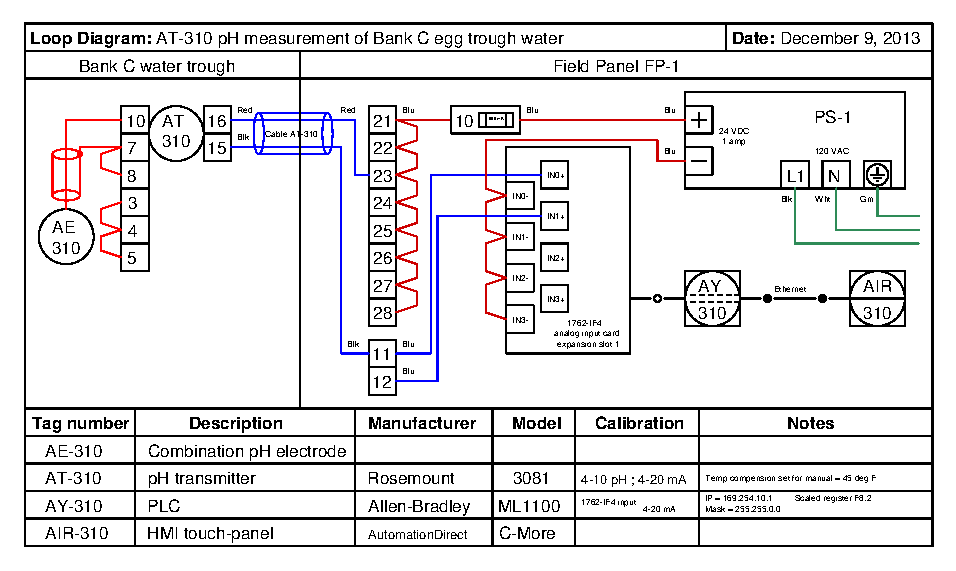
\includegraphics[width=15.5cm]{i00626x02.eps}$$
















\vfil \eject

\noindent
{\bf Lab questions}

\vskip 20pt

Suppose AIT-41 is a self-powered pH transmitter (i.e. with a 4-20 mA current {\it sourcing} output) and AAL/AAH-41 is an alarm module with a 4-20 mA input that is ``passive'' (i.e. does not supply loop power).  Sketch all connecting wires (and any other components) necessary to connect these two instruments together to form a working pH alarm system:

$$\includegraphics[width=15.5cm]{i00626x03.eps}$$

\vskip 30pt

 Explain how pH {\it buffer} solutions differ from any other chemical solution of known pH value, and how this quality especially qualifies the buffer to be used as a calibration standard.

\vskip 30pt

Calculate the {\it greatest} error for this carbon monoxide transmitter (in percent of span), based on the following As-Found calibration test results over its full range.  Be sure to specify the mathematical {\it sign} of the error value you calculate:

% No blank lines allowed between lines of an \halign structure!
% I use comments (%) instead, so that TeX doesn't choke.

$$\vbox{\offinterlineskip
\halign{\strut
\vrule \quad\hfil # \ \hfil & 
\vrule \quad\hfil # \ \hfil \vrule \cr
\noalign{\hrule}
%
% First row
{\bf Calibration gas} & {\bf Output signal} \cr
%
\noalign{\hrule}
%
% Another row
0 ppm & 4.03 mA \cr
%
\noalign{\hrule}
%
% Another row
25 ppm & 7.99 mA \cr
%
\noalign{\hrule}
%
% Another row
50 ppm & 11.94 mA \cr
%
\noalign{\hrule}
%
% Another row
75 ppm & 15.97 mA \cr
%
\noalign{\hrule}
%
% Another row
100 ppm & 20.02 mA \cr
%
\noalign{\hrule}
} % End of \halign 
}$$ % End of \vbox

\vskip 30pt

\filbreak

 Suppose AIR-310 registers 2.5 pH at all times, regardless of changes in the actual pH of the water in the Bank C trough.  A technician measures 0 VDC between terminals 21 and IN0$-$.  Identify one specific fault which could account for all the symptoms, as well as one specific component in this system which is definitely not to blame.  Be sure to specify ``open'' or ``shorted'' if your specified fault is electrical in nature:

$$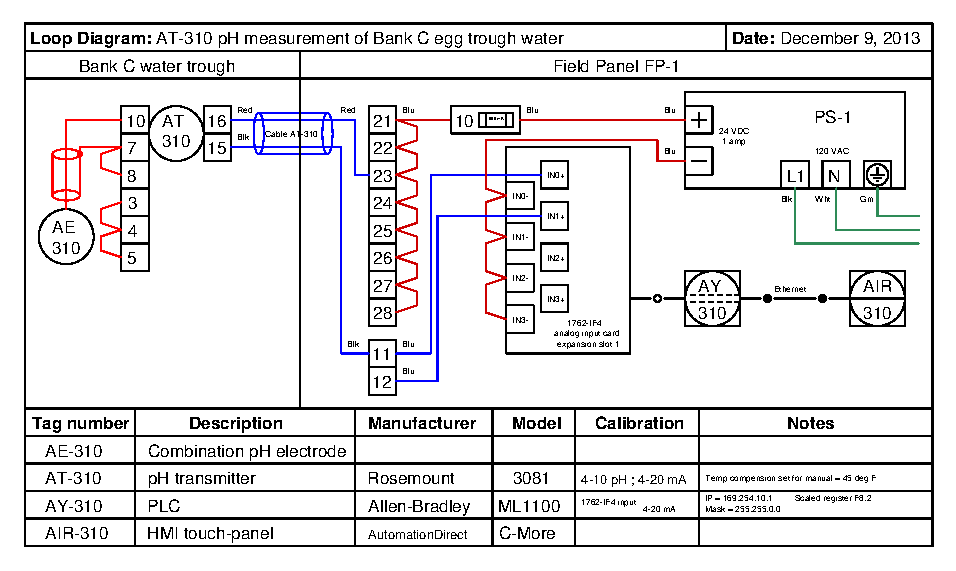
\includegraphics[width=15.5cm]{i00626x02.eps}$$


%INDEX% Lab exercise, analytical transmitter
%INDEX% Lab exercise, analyzer loop

\vfil \eject 



\oppgave{} 
% Copyright 2015, Tony R. Kuphaldt, released under the Creative Commons Attribution License (v 1.0)
% This means you may do almost anything with this work of mine, so long as you give me proper credit

\noindent
{\bf Lab Exercise}

\vskip 5pt

Your task is to build, document, and successfully operate a process controlled by a recording PID controller.  Several alternative process types exist and are documented in subsequent pages.  The working process you build will be used in future lab exercises this quarter to meet other learning objectives, which means you will {\it not} disassemble this project at the completion of these lab objectives as you normally would.

The following table of objectives show what you and your team must complete within the scheduled time for this lab exercise.  Note how some of these objectives are individual, while others are for the team as a whole:

\underbar{Objective completion table:}

% No blank lines allowed between lines of an \halign structure!
% I use comments (%) instead, so that TeX doesn't choke.

$$\vbox{\offinterlineskip
\halign{\strut
\vrule \quad\hfil # \ \hfil & 
\vrule \quad\hfil # \ \hfil & 
\vrule \quad\hfil # \ \hfil & 
\vrule \quad\hfil # \ \hfil & 
\vrule \quad\hfil # \ \hfil & 
\vrule \quad\hfil # \ \hfil & 
\vrule \quad\hfil # \ \hfil \vrule \cr
\noalign{\hrule}
%
% First row
{\bf Performance objective} & {\bf Grading} & {\bf 1} & {\bf 2} & {\bf 3} & {\bf 4} & {\bf Team} \cr
%
\noalign{\hrule}
%
% Another row
Choose process to build & mastery & -- & -- & -- & -- & \cr
%
\noalign{\hrule}
%
% Another row
Team meeting and prototype sketch & mastery & -- & -- & -- & -- & \cr
%
\noalign{\hrule}
%
% Another row
Circuit design challenge & mastery & & & & & -- -- -- -- \cr
%
\noalign{\hrule}
%
% Another row
Final loop diagram and system inspection & mastery & & & & & -- -- -- -- \cr
%
\noalign{\hrule}
%
% Another row
Process and Instrument Diagram (P\&ID) & mastery & & & & & -- -- -- -- \cr
%
\noalign{\hrule}
%
% Another row
Trend graph displays PV and Output & mastery & -- & -- & -- & -- &  \cr
%
\noalign{\hrule}
%
% Another row
Process exhibits good control behavior & mastery & -- & -- & -- & -- &  \cr
%
\noalign{\hrule}
%
% Another row
PV alarm(s) defined and enabled & mastery & -- & -- & -- & -- &  \cr
%
\noalign{\hrule}
%
% Another row
Lab question: Instrument connections & proportional &  &  &  &  & -- -- -- -- \cr
%
\noalign{\hrule}
%
% Another row
Lab question: Commissioning & proportional &  &  &  &  & -- -- -- -- \cr
%
\noalign{\hrule}
%
% Another row
Lab question: Mental math & proportional &  &  &  &  & -- -- -- -- \cr
%
\noalign{\hrule}
%
% Another row
Lab question: Diagnostics & proportional &  &  &  &  & -- -- -- -- \cr
%
\noalign{\hrule}
} % End of \halign 
}$$ % End of \vbox

The only ``proportional'' scoring in this activity are the lab questions, which are answered by each student individually.  A listing of potential lab questions are shown at the end of this worksheet question.  The lab questions are intended to guide your labwork as much as they are intended to measure your comprehension, and as such the instructor may ask these questions of your team day by day, rather than all at once (on a single day).

\vskip 10pt

{\bf It is essential that your team plans ahead what to accomplish each day.  A short (10 minute) team meeting at the beginning of each lab session is a good way to do this, reviewing what's already been done, what's left to do, and what assessments you should be ready for.  There is a lot of work involved with building, documenting, and troubleshooting these working instrument systems!}

As you and your team work on this system, you will invariably encounter problems.  You should always attempt to solve these problems as a team before requesting instructor assistance.  If you still require instructor assistance, write your team's color on the lab whiteboard with a brief description of what you need help on.  The instructor will meet with each team in order they appear on the whiteboard to address these problems.

$$\includegraphics[width=15.5cm]{i01558x01.eps}$$





\vfil \eject

\noindent
{\bf Lab Exercise -- choosing a process to build}

\vskip 5pt

There are a number of process types to choose from when selecting the one you will build with your team.  The only non-negotiable limitations is that the process must be safe, legal, and possible to complete in the time allotted for this lab.  What follows are some examples:

$$\includegraphics[width=15.5cm]{i01558x02.eps}$$

$$\includegraphics[width=15.5cm]{i01558x03.eps}$$

\filbreak

$$\includegraphics[width=15.5cm]{i01558x04.eps}$$

$$\includegraphics[width=15.5cm]{i01558x05.eps}$$

\filbreak

$$\includegraphics[width=15.5cm]{i01558x06.eps}$$

$$\includegraphics[width=15.5cm]{i01558x07.eps}$$

\noindent
Other process ideas include:

\begin{itemize}
\item{} Soldering iron temperature control (blowing air over tip with variable-speed fan).
\vskip 10pt
\item{} Draft pressure control (controlling very low air pressure inside of a box). 
\vskip 10pt
\item{} Pneumatic piston height control (using lengths of PVC pipe to build a simple piston/cylinder which may be used to lift small weights using modest air pressures).  A good way to control air pressure to the piston is to route the I/P transducer's output to a {\it volume booster} relay and let the relay's output directly drive the piston.  Piston height may be sensed using a flexible water tube attached to the piston rod, running to a stationary pressure transmitter.
\vskip 10pt
\item{} Sterno-fired air heat exchanger. 
\vskip 10pt
\item{} Miniature steam boiler.  {\it Note: this is an advanced project!}
\vskip 10pt
\item{} Air/Fuel ratio burner control.  {\it Note: this is an advanced project!}
\vskip 10pt
\item{} Servomechanism position control.  {\it Note: this is an advanced project!}
\vskip 10pt
\item{} Inverted pendulum balance.  {\it Note: this is a \underbar{very} advanced project!}
\end{itemize}






\vfil \eject

\noindent
{\bf Lab Exercise -- team meeting, prototype sketch, and instrument selection}

\vskip 5pt

An important first step in completing this lab exercise is to {\bf meet with your instructor} as a team to discuss safety concerns, team performance, and specific roles for team members.  If you would like to emphasize exposure to certain equipment (e.g. use a particular type of control system, certain power tools), techniques (e.g. fabrication), or tasks to improve your skill set, this is the time to make requests of your team so that your learning during this project will be maximized.

\vskip 10pt

An absolutely essential step in completing this lab exercise is to work together as a team to {\bf sketch a prototype diagram} showing what you intend to build.  This usually takes the form of a simple electrical schematic and/or loop diagram showing all electrical connections between components, as well as any tubing or piping for fluids.  This prototype sketch need not be exhaustive in detail, but it does need to show enough detail for the instructor to determine if all components will be correctly connected for their safe function.

For example, if you intend to connect field devices to a PLC (Programmable Logic Controller), your prototype sketch must show how those devices will connect to typical input/output terminals on the PLC, where electrical power will be supplied, etc.  Prototype sketches need not show all intermediary connections between components, such as terminal blocks in junction boxes between the field device and the controller.

You should practice good problem-solving techniques when creating your prototype sketch, such as consulting equipment manuals for information on component functions and marking directions of electric current, voltage polarities, and identifying electrical sources/loads.  Use this task as an opportunity to strengthen your analytical skills!  Remember that you will be challenged in this program to do all of this on your own (during ``capstone'' assessments), so do not make the mistake of relying on your teammates to figure this out for you -- instead, treat this as a problem {\it you} must solve and compare your results with those of your teammates.

Your team's prototype sketch is so important that the instructor will demand you provide this plan before any construction on your team's working system begins.  {\it Any team found constructing their system without a verified plan will be ordered to cease construction and not resume until a prototype plan has been drafted and approved!}  Similarly, you should not deviate from the prototype design without instructor approval, to ensure nothing will be done to harm equipment by way of incorrect connections.  Each member on the team should have ready access to this plan (ideally possessing their own copy of the plan) throughout the construction process.  Prototype design sketching is a skill and a habit you should cultivate in school and take with you in your new career.

\vskip 10pt

When selecting field instruments for this lab exercise, choose a {\it transmitter} suitable for measuring your process variable, and likely an {\it I/P converter} used to convert the controller's 4-20 mA output signal into an air pressure that a control valve may operate on.  Electronic process controllers are in several locations throughout the lab, ready to be used for controlling processes.  Your instructor will help you select appropriate instruments for the process you have chosen.

You may also need a {\it data acquisition unit}, or {\it DAQ} to function as a trend recorder.  When used with a personal computer and connected properly to the loop circuit, a DAQ unit will provide graphical displays of loop variables over time.  Students usually find the connection of a DAQ unit to their loop controller to be the trickiest part of their loop wiring.  You will need to consult the manufacturer documentation on the DAQ unit as well as the field instruments and controller in order to figure out how to wire them together.  Even if your process controller already provides trending capability, you may find connection of a DAQ unit to your loop circuits a useful exercise because the ability to quickly connect and use DAQ hardware and software to monitor electrical parameters in a system is a valuable diagnostic skill in this career.

You will find your teammates who have already taken the Measurement course series (INST24X) will be very helpful in showing you how to check, configure, calibrate, and install the measuring instrument(s) you will need for your process!

\vskip 10pt

{\bf Planning a functioning system should take no more than an hour if the team is working efficiently, and will save you hours of frustration (and possible component destruction!).}






\vfil \eject

\noindent
{\bf Lab Exercise -- circuit design challenge}

\vskip 5pt

Your instructor will choose one 4-20 mA field instrument and one control system from the lists shown below, for which you must sketch an accurate circuit diagram showing how the two instruments would connect to each other.  If this interconnection between controller and field instrument requires additional electrical components to function (e.g. DC or AC power source, precision 250 $\Omega$ resistor, diode, relay, etc.), those must be incorporated into your diagram as well.  Instruction manuals for all instrument listed are available on the electronic Instrumentation Reference for your convenience.  When your sketch is complete, you must show the relevant manual pages to your instructor for verification of correct connections.

This exercise tests your ability to locate appropriate information in technical manuals and design a correct 4-20 mA analog signal circuit for a given pair of instruments.  The electronic Instrumentation Reference will be available to you in order to answer this question.

\vskip 10pt

Since all 4-20 mA ``loops'' are basically series DC circuits, it is highly recommended that you approach their design the same as for any other DC circuit: carefully identify all {\it sources} and {\it loads} in the circuit, trace directions of all currents, and mark the polarities of all voltages.  Most of the mistakes made in this type of circuit design challenge may be remedied by careful consideration of these specific circuit-analysis details.

%%%%%%%%%%%%%%%%%%%%%%%%%%%%%%%
\vskip 10pt
\filbreak
\hbox{ \vrule
\vbox{ \hrule \vskip 3pt
\hbox{ \hskip 3pt
\vbox{ \hsize=5in \raggedright

\noindent \centerline{\bf 4-20 mA transmitter options}
\begin{itemize}
\item{} Pressure

	\begin{itemize}
	\item{} Yokogawa DPharp EJX110A or EJX910 
	\item{} Honeywell ST3000
	\end{itemize}
\vskip 2pt
\item{} Level
\vskip 2pt

\item{} Temperature
		\begin{itemize}
		\item{} Foxboro RTT15 or RTT30
		\item{} Moore Industries SPT with sourcing (4-wire) 4-20 mA output
		\item{} Moore Industries SPT with sinking (2-wire) 4-20 mA output
		\item{} Moore Industries TRX or TDY
		%\item{} Honeywell STT173
		\end{itemize}
\vskip 2pt
\item{} Flow

\vskip 2pt
\item{} Analytical
	\begin{itemize}
	\item{} Daniel 700 gas chromatograph (4 analog output channels)
	\item{} Foxboro 876PH (pH/ORP/ISE)
	\end{itemize}
\end{itemize}

} \hskip 3pt}%
\vskip 5pt \hrule}%
\vrule}
%%%%%%%%%%%%%%%%%%%%%%%%%%%%%%%




%%%%%%%%%%%%%%%%%%%%%%%%%%%%%%%
\vskip 10pt
\filbreak
\hbox{ \vrule
\vbox{ \hrule \vskip 3pt
\hbox{ \hskip 3pt
\vbox{ \hsize=5in \raggedright

\noindent \centerline{\bf Controller options}
\begin{itemize}
\item{} Monolithic

\begin{itemize}
	\item{} Siemens 353
	\item{} Foxboro 716C
	\item{} Foxboro 718TC
	\item{} Foxboro 762CNA 
	\item{} Moore Industries 535
	\item{} Honeywell UDC2300
	\item{} Honeywell UDC3500 
\end{itemize}
\vskip 2pt
\item{} Modular -- {\it you choose the appropriate I/O module}
\begin{itemize}

	\item{} Emerson ROC800 SCADA/RTU 
\end{itemize}
\vskip 2pt
\item{} Distributed Control System (DCS) -- {\it you choose the appropriate I/O module}
\begin{itemize}

	\item{} Emerson DeltaV with S-series I/O 
	\item{} Honeywell Experion with 2MLF series I/O 
\end{itemize}
\vskip 2pt
\item{} Programmable Logic Controller (PLC) -- {\it you choose the appropriate I/O module}
\begin{itemize}

	\item{} Rockwell ControlLogix (catalog number 1756)
	\item{} Rockwell CompactLogix (catalog number 1769)
\end{itemize}

\end{itemize}

} \hskip 3pt}%
\vskip 5pt \hrule}%
\vrule}
%%%%%%%%%%%%%%%%%%%%%%%%%%%%%%%




%%%%%%%%%%%%%%%%%%%%%%%%%%%%%%%
\vskip 10pt
\filbreak
\hbox{ \vrule
\vbox{ \hrule \vskip 3pt
\hbox{ \hskip 3pt
\vbox{ \hsize=5in \raggedright

\noindent \centerline{\bf 4-20 mA Final Control Element options}
\begin{itemize}
\item{} Pneumatic control valve positioners
\begin{itemize}

\item{} Fisher DVC6000 positioner 
\end{itemize}
\vskip 2pt
\item{} Electrically actuated valves (MOV)
\begin{itemize}

\item{} Rotork AQ with Folomatic controller 
\end{itemize}
\vskip 2pt
\item{} AC motor drives (VFD)
\begin{itemize}

\item{} Automation Direct GS1 
\end{itemize}
\end{itemize}

} \hskip 3pt}%
\vskip 5pt \hrule}%
\vrule}
%%%%%%%%%%%%%%%%%%%%%%%%%%%%%%%


\vfil

Study reference: the ``Analog Electronic Instrumentation'' chapter of {\it Lessons In Industrial Instrumentation}, particularly the section on HART.

\vskip 10pt

Note: a very effective problem-solving strategy for determining how to connect different components together to create a working 4-20 mA current loop is to first identify whether each component acts as a {\it source} or a {\it load} in that loop circuit.  Then, label voltage polarities (+ , $-$) and directions of current accordingly.  Knowing which way current must flow through each component and which polarity each voltage must have is key to ensuring the inter-component connections are correct.








\vfil \eject

\noindent
{\bf Lab Exercise -- building the system}

\vskip 5pt

The Instrumentation lab is set up to facilitate the construction of working instrument ``loops,'' with over a dozen junction boxes, pre-pulled signal cables, and ``racks'' set up with 2-inch vertical pipes for mounting instruments.  These racks also provide structure for building physical processes, with more than enough weight-bearing capacity to hold any process vessels and equipment.  The only wires you should need to install to build a working system are those connecting the field instrument to the nearest junction box, and then small ``jumper'' cables connecting different pre-installed cables together within intermediate junction boxes.

After getting your prototype sketch approved by the instructor, you are cleared to begin building your system.  Instruments attach to 2-inch pipes using special brackets and U-bolts.  These brackets and U-bolts are located in the instrument storage area.  

Select a specific loop controller for your system.  Your instructor may choose the controller for your team, to ensure you learn more than one type of controller during the course of a quarter.

Finally, your process control system needs to have a loop number, so all instruments may be properly labeled.  This loop number needs to be unique, so that another team does not label their instruments and cables the same as yours.  One way to make your loop number unique is to use the equivalent resistor color-code value for your team's color in the loop number.  For example, if you are the ``Red'' team, your loop number could be ``2''. 

\vskip 10pt

{\bf Common mistakes:}

\begin{itemize}
\item{} Neglecting to consult the manufacturer's documentation for field instruments (e.g. how to wire them, how to calibrate them).
\item{} Mounting the field instrument(s) in awkward positions, making it difficult to reach connection terminals or to remove covers when installed.
\item{} Improper pipe/tube fitting installation (e.g. trying to thread tube fittings into pipe fittings and vice-versa).
\item{} Failing to tug on each and every wire where it terminates to ensure a mechanically sound connection.
\item{} Students working on portions of the system in isolation, not sharing with their teammates what they did and how.  It is important that the whole team learns all aspects of their system!
\end{itemize}

\vskip 10pt

{\bf Building a functioning process complete with instrumentation for control typically takes one or two sessions (3 hours each) if all components are readily available and the team is working efficiently!}





\vfil \eject

\noindent
{\bf Lab Exercise -- documenting the system}

\vskip 5pt

Each student must sketch their own {\it loop diagram} and their own {\it P\&ID} for their team's system, following proper ISA conventions.  The P\&ID documents the flow of fluid and materials in your process plus the general control strategy.  The loop diagram documents all wiring and tube connections between instruments.  Although the two diagrams reinforce one another and might possibly be combined into one, the industry standard is to use two separate diagrams.

Sample loop diagrams are shown in the next question in this worksheet.  These loop diagrams must be {\it comprehensive} and {\it detailed}, showing every wire connection, every cable, every terminal block, range points, etc.  The principle to keep in mind here is to make the loop diagram so complete and unambiguous that anyone can follow it to see what connects to what, even someone unfamiliar with industrial instrumentation.  In industry, loops are often constructed by contract personnel with limited understanding of how the system is supposed to function.  The loop diagrams they follow must be so complete that they will be able to connect everything properly without necessarily understanding how it is supposed to work.

Every instrument and every signal cable in your loop needs to be properly labeled with an ISA-standard tag number.  An easy way to do this is to wrap a short piece of masking tape around each cable (and placed on each instrument) then writing on that masking tape with a permanent marker.  Although no industry standard exists for labeling signal cables, a good recommendation is to label each two-wire cable with the tag number of the field instrument it goes to.  Thus, every length of two-wire cable in a pressure transmitter circuit should be labeled ``PT-$x$'' (where ``$x$'' is the loop number), every flow control valve should be labeled ``FV-$x$'', etc.  Remember that the entire loop is defined by the process variable it measures: if the PV is {\it temperature} then the transmitter with be a {\it T}T, the control valve will be a {\it T}V, the controller with be a {\it T}C, etc.

When your entire team is finished drafting your individual loop diagrams, call the instructor to do an inspection of the loop.  Here, the instructor will have students take turns going through the entire loop, with the other students checking their diagrams for errors and omissions along the way.  During this time the instructor will also inspect the quality of the installation, identifying problems such as frayed wires, improperly crimped terminals, poor cable routing, missing labels, lack of wire duct covers, etc.  The team must correct all identified errors in order to receive credit for their system.  

After successfully passing the inspection, each team member needs to place their loop diagram in the diagram holder located in the middle of the lab behind the main control panel.  When it comes time to troubleshoot another team's system, this is where you will go to find a loop diagram for that system!

The P\&ID's will be submitted to the instructor for inspection as well, but the process itself need not be inspected again.

\vskip 10pt

{\bf Common mistakes:}

\begin{itemize}
\item{} Forgetting to label all signal wires (see example loop diagrams).
\item{} Forgetting to label all field instruments with their own tag names (e.g. PT-83).
\item{} Forgetting to note all wire colors.
\item{} Forgetting to put your name on the loop diagram!
\item{} Using non-standard tags for instruments rather than ISA 5.1 standard notation.
\item{} Basing your diagram off of a team-mate's diagram, rather than closely inspecting the system for yourself.
\item{} Not placing loop sheet instruments in the correct orientation (field instruments on the left, control room instruments on the right).
\end{itemize}

\vskip 10pt

{\bf Creating and inspecting accurate loop diagrams should take no more than one full lab session (3 hours) if the team is working efficiently!  Creating and inspecting accurate P\&IDs will take more time, but not an entire lab session (3 hours).}







\vfil \eject

\noindent
{\bf Lab Exercise -- operating the system}

\vskip 5pt

All networked loop controllers in the lab (DCS, DDC, PLC, single-loop networked) provide graphing functionality so that you may plot your process variable (PV) and output values over time.  This graphical data is essential for tuning PID-controlled loops.  If you happen to be using a controller that does not provide graphing capability, your team must attach a trend recorder and/or a data acquisition unit (plus a personal computer) to the necessary signal cables so that these values are recorded over time.

PID tuning is a subject worthy of its own course, and so you will not be expected to achieve perfect control on your process.  You will find, however, that one of the best ways to learn PID tuning is by ``playing'' with your process as it responds to different tuning parameters entered into the loop controller.  The expectation for ``good control behavior'' in the context of this lab exercise is for the loop to exhibit response that is no less stable following large setpoint changes than the classic ``quarter-wave damping'' described by Ziegler and Nichols in their 1942 paper.

\vskip 10pt

Most student-built processes are quite safe to operate.  However, if your process harbors any unique hazards (e.g. overflowing water may present a slip hazard, overheated oven may cause materials to smoke or burn), you must be aware of these hazards and limit everyones' exposure to them.  All team members for each process must be familiar with the inherent hazards of their process and how to mitigate them.  One operational step to help avoid problems is to configure the controller for {\it setpoint limits} preventing the setpoint value from being placed at ``dangerous'' values in automatic mode.  Just what these setpoint limit values should be set to varies with the process and the team's experience operating it.

As your time with the process builds, you will no doubt arrive at ideas for improving it.  Feel free to work with your team to optimize the process in any way you see fit.  The goal is to have your process as robust and ``problem-free'' as possible for other teams to use it in later coursework!

\vskip 10pt

After you have built and tuned your process, you should identify and configure alarm values for the controller's PV display.  Most controllers have PV alarm capability built in, signaling a condition of excessive or insufficient PV if those alarm points are ever tripped.  You need to set at least a high alarm on the PV so that when other teams come after you to re-tune your process, they have some ``guidepost'' showing them what PV value(s) they should not exceed!  If your team has enough time, feel free to connect an actual alarm indicator light and/or audible buzzer to your control system that turns on (and latches) if an alarm point is exceeded.

A tendency of students when they first learn to tune PID control loops is to proceed carelessly because they know the ``toy'' processes they are learning to tune aren't going to harm anything if their PVs go out of bounds.  While this assumption might be true for your team's process, it is not good to form or reinforce bad habits.  Thus, the inclusion of alarm point(s) on your process PV -- especially if connected to some form of signaling device that is annoying and/or embarrassing to trip such as a loud buzzer -- makes for a better teaching tool for others learning PID tuning!



\vfil \eject

\centerline{\bf Troubleshooting PID-controlled processes}

\vskip 10pt

It is quite likely during the testing and operation of your control loop that problems will develop.  The following advice is given to assist you in your diagnostic efforts, to quickly identify which portion(s) of your control loop might be at fault.

\vskip 10pt

Recall that every feedback control loop consists of four basic elements: an element that {\it senses} the process variable (e.g. primary sensing element, transmitter), an element that {\it decides} what how to regulate this process variable (e.g. a PID controller), an element that {\it influences} the process variable (e.g. a control valve, motor drive, or some other final control device), and finally the process itself which {\it reacts} to the final control device's actions:

$$ \includegraphics[width=15.5cm]{i01558x09.eps}$$

\noindent
You can check each element of your feedback control loop by comparing its input with its output to see if each element is doing what it should:

\begin{itemize}
\item{$(1)$} \underbar{\bf Decision-making:} Carefully examine the controller faceplate, looking at the values of PV, SP, and Output.  Is the controller taking appropriate action to force PV equal to SP?  In other words, is the Output signal at a value you would expect if the controller were functioning properly to regulate the process variable at setpoint?  If so, then the controller's action and tuning are most likely not at fault.  If not, then the problem definitely lies with the controller.
\item{$(2)$} \underbar{\bf Sensing:} Compare the controller's displayed value for PV with the actual process variable value as indicated by local gauges, by feel, or by any other means of detection.  If there is good correspondence between the controller's PV display and the real process variable, then there probably isn't anything wrong with the measurement portion of the control loop (e.g. transmitter, impulse lines, PV signal wiring, analog input of controller, etc.).  If the displayed PV disagrees with the actual process variable value, then something is definitely wrong here.
\item{$(3)$} \underbar{\bf Influencing:} Compare the controller's displayed value for Output with the actual status of the final control element.  If there is good correspondence between the controller's Output display and the FCE's status, then there probably isn't anything wrong with the output portion of the control loop (e.g. FCE, output signal wiring, analog output of controller, etc.).  If the controller Output value differs from the FCE's state, then something is definitely wrong here.
\item{$(4)$} \underbar{\bf Reacting:} Compare the process variable value with the final control element's state.  Is the process doing what you would expect it to?  If so, the problem is most likely not within the process (e.g. manual valves, relief valves, pumps, compressors, motors, and other process equipment).  If, however, the process is not reacting the way you would expect it to given the final control element's state, then something is definitely awry with the process itself.
\end{itemize}






\vfil \eject

\centerline{\bf A crude closed-loop PID tuning procedure}

\vskip 10pt

Tuning a PID controller is something of an art, and can be quite daunting to the novice.  What follows is a primitive (oversimplified for some situations!) procedure you can apply to many processes.

\vskip 10pt

\noindent
{\bf Step 1}

\underbar{Understand the process you are trying to control.}  If you do not have a fundamental grasp on the nature of the process you're controlling, it is pointless -- even dangerous -- to change controller settings.  Here is a simple checklist to cover before touching the controller:

\begin{itemize}
\item{} What is the process variable and how is it measured?
\item{} What is the final control element, and how does it exert control over the process variable?
\item{} What safety hazards exist in this process related to control (e.g. danger of explosion, solidification, production of dangerous byproducts, etc.)?  
\item{} How far am I allowed to ``bump'' the process while I tune the controller and monitor the response?
\item{} How is the controller mode switched to ``manual,'' just in case I need to take over control?
\item{} In the event of a dangerous condition caused by the controller, how do you shut the process down?
\end{itemize}

\vskip 10pt

\noindent
{\bf Step 2}

\underbar{Understand what the settings on the controller do.}  Is your controller configured for gain or proportional band?  Minutes per repeat or repeats per minute?  Does it use reset windup limits?  Does rate respond to error or PV alone?  You had better understand what the PID values do to the controller's action if you are going to decide which way (and how much) to adjust them!  Back in the days of analog electronic and pneumatic controllers, I would recommend to technicians that they draw little arrow symbols next to each adjustment knob showing which way to turn for more aggressive action -- this way they wouldn't get mixed up figuring out gain vs PB, rep/min vs min/rep, etc.: all they had to think of is ``more'' or ``less'' of each action.

\vskip 10pt

\noindent
{\bf Step 3}

\underbar{Manually ``bump'' the manipulated variable (final control element) to learn how the process responds.}  In manual mode, {\it you} are the controller!  What you need to do is adjust the process to learn how it responds: is it an integrating process, a self-regulating process, or a runaway process?  Is there significant dead time or hysteresis?  Is the response linear and consistent?  Many process control problems are caused by factors other than the controller, and this ``manual test'' step is a key diagnostic technique for assessing these other factors.

\vskip 10pt

\noindent
{\bf Step 4}

\underbar{Set the PID constants to ``minimal'' settings and switch to automatic mode.}  This means gain less than 1, no integral action (0 rep/min or maximum min/rep), no derivative action, and no filtering (i.e. damping).

\vskip 10pt

\noindent
{\bf Step 5}

\underbar{``Bump'' the setpoint and watch the controller's response.}  This tests the controller's ability to manage the process on its own.  What you want is a response that is reasonably fast without overshooting or undershooting too much, and without undue cycling.  The nature of the process and the constraints of quality standards will dictate what is ``too much'' response time, over/undershoot, and cycling.

\vskip 10pt

\noindent
{\bf Step 6}

\underbar{Increase or decrease the control action aggressiveness according to the results of Step 5.}

\vskip 10pt

\noindent
{\bf Step 7}

\underbar{Repeat steps 5 and 6 for P, I, and D, one at a time, in that order.}  In other words, tune the controller first to act as a P-only controller, then add integral (PI control), then derivative (PID), each as needed.

\filbreak

\vskip 10pt

\noindent
{\bf Step 8}

\underbar{``Bump'' a load in the process and watch the controller's response.}  This tests the controller's ability to manage variations in process load over time.  A controller's response to load changes will often differ from its response to setpoint changes.  You still want controller response that is reasonably fast without overshooting or undershooting too much, and without undue cycling.  However, you may have to find some compromise in tuning between good setpoint response and good load response.  How you decide that compromise depends on whether the controller really needs to respond mostly to setpoint changes (e.g. the slave controller of a cascade loop) or to load changes.

\vskip 10pt

\noindent
{\bf Step 9}

\underbar{Increase or decrease the control action aggressiveness according to the results of Step 8.}

\vskip 10pt

\noindent
{\bf Step 10}

\underbar{Repeat steps 8 and 9 for P, I, and D, one at a time, in that order.}  In other words, tune the controller first to act as a P-only controller, then add integral (PI control), then derivative (PID), each as needed.

\vskip 10pt


\centerline{\bf Caveats}

\vskip 10pt

The procedure described here is {\it very} crude, and should only be applied as a student's first foray into PID tuning, on a safe ``demonstration'' process.  It assumes that the process responds predominantly to proportional (P-only) action, which may not be true for some processes.  It also gives no specific advice for tuning based on the results of step 3, which is the mark of an experienced PID tuner.  With study, practice, and time, you will learn what types of processes respond best to P, I, and D actions, and then you will be able to intelligently choose what parameters to adjust, and what closed-loop behaviors to look for.

\vskip 10pt







\vfil \eject

\noindent
{\bf Lab questions}

\vskip 5pt

\begin{itemize}
\item{} {\bf Instrument connections}
\item{} Determine correct wire connections between instruments to create a working 4-20 mA loop circuit, based on diagrams of instruments with terminals labeled
\item{} Correctly determine all electrical sources and loads, as well as all voltage polarities and current directions in a 4-20 mA loop circuit, based on diagrams of instruments with terminals labeled
\end{itemize}

\filbreak

\begin{itemize}
\item{} {\bf Commissioning and Documentation}
\item{} Identify and explain the distinction between {\it direct} and {\it reverse} control modes in the loop controller
\item{} Identify some of the main {\it loads} in your process, and explain how they may be varied while the process is running
\item{} Describe how to connect a loop calibrator to measure current output by a loop-powered (2-wire) transmitter
\item{} Describe how to connect a loop calibrator to measure current output by a controller
\item{} Describe how to connect a loop calibrator to simulate current coming from a loop-powered (2-wire) transmitter
\item{} Describe how to connect a loop calibrator to simulate current coming from a self-powered (4-wire) transmitter
\item{} Describe how to connect a loop calibrator to stroke a control valve
\end{itemize}

\filbreak

\begin{itemize}
\item{} {\bf Mental math} (no calculator allowed!)
\item{} Convert a proportional band value into a gain value, or vice-versa
\item{} Convert a repeats/(minute or second) integral value into a (minutes or seconds)/repeat integral value, or vice-versa
\item{} Calculate the pneumatic pressure in a 3-15 PSI range corresponding to $x$ percent.
\item{} Calculate the electrical current in a 4-20 mA range corresponding to $x$ percent.
\item{} Calculate the electrical voltage in a 1-5 volt range corresponding to $x$ percent.
\item{} Calculate the percentage value of a pneumatic pressure signal $x$ PSI in a 3-15 PSI range.
\item{} Calculate the percentage value of an electrical current signal $x$ mA in a 4-20 mA range.
\item{} Calculate the percentage value of an electrical voltage signal $x$ volts in a 1-5 volt range.
\end{itemize}

\filbreak

\begin{itemize}
\item{} {\bf Diagnostics}
\item{} Explain how to distinguish an ``open'' cable fault from a ``shorted'' cable fault using only a voltmeter (no current or resistance measurement, but assuming you are able to break the circuit to perform the test)
\item{} Explain how to use the ``manual'' mode of a process controller as a diagnostic test to check for problems in a control system
\item{} Determine whether or not a given diagnostic test will provide useful information, given a set of symptoms exhibited by a failed system
\item{} Identify at least two plausible faults given the results of a diagnostic test and a set of symptoms exhibited by a failed system
\item{} Propose a diagnostic test for troubleshooting a failed system and then explain the meanings of two different test results
\end{itemize}



\underbar{file i01558}
\vskip 10pt \filbreak 





\svar{} 


\vskip 10pt \filbreak 





\notes{} 

\noindent
{\bf Loop diagrams / inspections:}

I strongly recommend checking off students' loop diagrams while you inspect their loop (checking for secure wiring, proper tubing, good conduit installation, etc.) with them.  Have all team members take you on a ``tour'' of their completed loop, with each team member explaining a different portion of the loop you select while using their own loop diagram as a guide.  While a student is explaining their section of the loop, you can check the other students' loop diagrams for accuracy.  This not only saves time by consolidating the tasks of loop inspection and loop diagram verification, but it also ensures students can actually relate their loop diagrams to the loop they have built and articulate that understanding to you.











\vfil \eject

\noindent
{\bf Lab questions}

\vskip 20pt
\begin{itemize}
\item{$(1)$} Sketch wire connections so that pressure applied to the DP transmitter will register on the ammeter:

$$\includegraphics[width=15.5cm]{i01558x10.eps}$$

\vskip 20pt

\item{$(2)$} Sketch how to connect a loop calibrator to {\it simulate} current from TT-14 in this circuit:

$$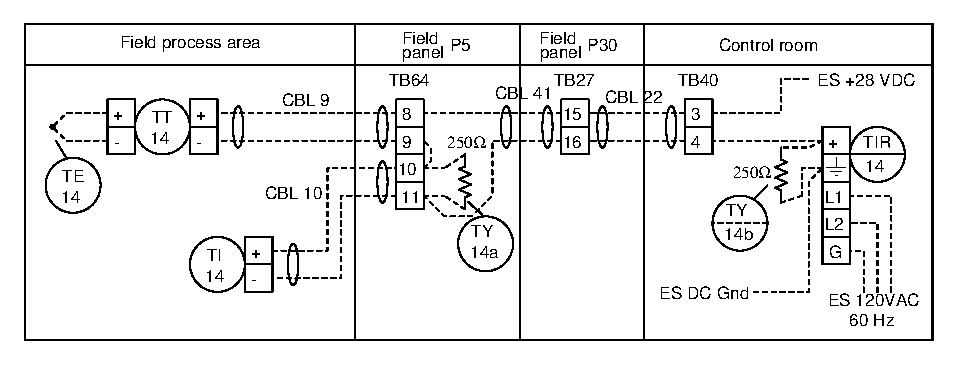
\includegraphics[width=15.5cm]{i01558x11.eps}$$

\vskip 20pt

\item{$(3)$} Calculate the percentage value of a 2.3 volt electrical signal in a 1-5 volt range.

\vskip 20pt

\item{$(4)$} Suppose the controller registers 103\% PV in this process, and the operators cannot change this even when they place the controller in manual mode with $-5$\% output.  Identify one possible fault, as well as one impossible fault, with regard to these symptoms.  Be specific in your identification: both the location (which component) and nature (e.g. open, shorted, plugged) of each fault.  

$$\includegraphics[width=15.5cm]{i01558x08.eps}$$
\end{itemize}











\vfil \eject

\noindent
{\bf Lab questions}

\vskip 20pt
\begin{itemize}
\item{$(1)$} Sketch wire connections so that pressure applied to the DP transmitter will register on the ammeter:

$$\includegraphics[width=15.5cm]{i01558x12.eps}$$

\vskip 20pt

\item{$(2)$} Sketch how to connect a loop calibrator to {\it measure} current coming from TT-14 in this circuit:

$$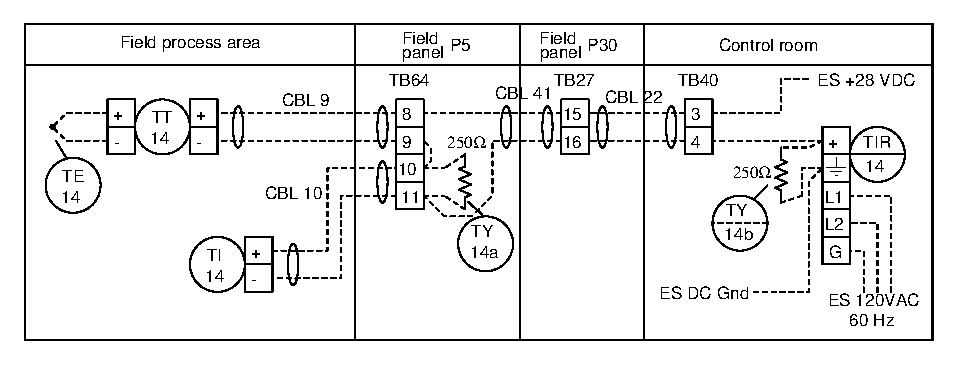
\includegraphics[width=15.5cm]{i01558x11.eps}$$

\vskip 20pt

\item{$(3)$} Calculate the percentage value of a 14.5 mA electrical signal in a 4-20 mA range.

\vskip 20pt

\item{$(4)$} Suppose the PV and SP (as displayed by the controller) do not match: with a 50\% setpoint, the process variable value remains at 62\% with the controller in automatic mode.  Identify one possible fault, as well as one impossible fault, with regard to these symptoms.  Be specific in your identification: both the location (which component) and nature (e.g. open, shorted, plugged) of each fault.  

$$\includegraphics[width=15.5cm]{i01558x08.eps}$$

\end{itemize}

%INDEX% Lab exercise, building a complete process control loop

\vfil \eject 



\oppgave{} 
% Copyright 2010, Tony R. Kuphaldt, released under the Creative Commons Attribution License (v 1.0)
% This means you may do almost anything with this work of mine, so long as you give me proper credit

\noindent
{\bf Lab Exercise}

\vskip 5pt

Your team's task is to build a complete, working process controlled by a networked digital controller or distributive control system.  Options include single-loop controllers connected to a workstation via network cabling, networked PLCs implementing PID control, DDC (building automation control) units, or a DCS.  When you operate your system, you must demonstrate operator control (e.g. setpoint changes, auto/manual mode, etc.) exercised remotely through a network computer connection to your process controller.

Each instrument in the loop should be labeled with a proper tag name (e.g. ``LT-59'' for a level transmitter), with all instruments in each loop sharing the same loop number.  Write on pieces of masking tape to make simple labels for all the instruments and signal lines.

After constructing the entire control loop, you will ``tune'' the P, I, and D settings of your controller so that it exhibits good control behavior (defined here as quarter-wave damping or better).

\vskip 10pt

\underbar{Objective completion table:}

% No blank lines allowed between lines of an \halign structure!
% I use comments (%) instead, so that TeX doesn't choke.

$$\vbox{\offinterlineskip
\halign{\strut
\vrule \quad\hfil # \ \hfil & 
\vrule \quad\hfil # \ \hfil & 
\vrule \quad\hfil # \ \hfil & 
\vrule \quad\hfil # \ \hfil & 
\vrule \quad\hfil # \ \hfil & 
\vrule \quad\hfil # \ \hfil & 
\vrule \quad\hfil # \ \hfil \vrule \cr
\noalign{\hrule}
%
% First row
{\bf Performance objective} & {\bf Grading} & {\bf 1} & {\bf 2} & {\bf 3} & {\bf 4} & {\bf Team} \cr
%
\noalign{\hrule}
%
% Another row
Choose process to build & mastery & -- & -- & -- & -- & \cr
%
\noalign{\hrule}
%
% Another row
Locate and navigate manual for controller & mastery & -- & -- & -- & -- & \cr
%
\noalign{\hrule}
%
% Another row
Loop diagram and process inspection & mastery & & & & & -- -- -- -- \cr
%
\noalign{\hrule}
%
% Another row
Process exhibits good control behavior & mastery & -- & -- & -- & -- &  \cr
%
\noalign{\hrule}
%
% Another row
Lab question: Selection/testing & proportional &  &  &  &  & -- -- -- -- \cr
%
\noalign{\hrule}
%
% Another row
Lab question: Commissioning & proportional &  &  &  &  & -- -- -- -- \cr
%
\noalign{\hrule}
%
% Another row
Lab question: Mental math & proportional &  &  &  &  & -- -- -- -- \cr
%
\noalign{\hrule}
%
% Another row
Lab question: Diagnostics & proportional &  &  &  &  & -- -- -- -- \cr
%
\noalign{\hrule}
} % End of \halign 
}$$ % End of \vbox

Each student will be asked to correctly answer a ``lab question'' from each of the four categories (examples shown on the next page).  These lab questions serve as a guide to knowledge and skills all team members should be learning as they progress through the lab exercise.  The instructor may quiz students on these questions at any appropriate time before the lab exercise is complete.

\vfil \eject

\noindent
\underbar{Lab Questions} 

\begin{itemize}
\item{} {\bf Selection and Initial Testing}
\item{} Identify all inputs and outputs on the field instruments (transmitter and FCE)
\item{} Explain the meanings of the various ratings specified on the instrument nameplate
\item{} Identify in the manufacturer documentation where to connect signal wires to the field instrument (transmitter or FCE)
\item{} Explain what types of test equipment were used to validate the operation of the field instrument (transmitter or FCE)
\item{} Explain how you could perform rudimentary tests of instrument function using simple test equipment (multimeter, air pumps, pressure gauges, resistors, batteries, etc.)
\end{itemize}

\filbreak

\begin{itemize}
\item{} {\bf Commissioning and Documentation}
\item{} Demonstrate how to isolate potentially hazardous energy in your system ({\it lock-out, tag-out}) and also how to safely verify the energy has been isolated prior to commencing work on the system
\item{} Demonstrate how to use a loop calibrator to measure/source/simulate signal current
\item{} Demonstrate proper wrench selection and use on nuts, bolts, and/or tube fittings
\item{} Identify the network connection(s) used to remotely access controller variables from a PC (e.g. IP addresses, Ethernet connections, Modbus networks and addresses, etc.)
\item{} Identify multiple locations (referencing a loop diagram) you may measure various 4-20 mA instrument signals in the system
\item{} Identify multiple locations (referencing a loop diagram) you may connect HART communicator in the system
\end{itemize}

\filbreak

\begin{itemize}
\item{} {\bf Mental math} (no calculator allowed!)
\item{} Determine allowable calibration error of instrument (e.g. +/- 0.5\% for an instrument ranged 200 to 500 degrees)
\item{} Convert 4-20 mA signal into a percentage of span (e.g. 13 mA = \underbar{\hskip 20pt}\%)
\item{} Convert percentage of span into a 4-20 mA signal value (e.g. 70\% = \underbar{\hskip 20pt} mA)
\item{} Convert 3-15 PSI signal into a percentage of span (e.g. 11 PSI = \underbar{\hskip 20pt}\%)
\item{} Convert percentage of span into a 3-15 PSI signal value (e.g. 40\% = \underbar{\hskip 20pt} PSI)
\end{itemize}

\filbreak

\begin{itemize}
\item{} {\bf Diagnostics}
\item{} Given a particular component or wiring fault ({\it instructor specifies type and location}), what symptoms would the loop exhibit and why?
\item{} Explain why breaking a 4-20 mA loop could cause serious problems in an actual instrument loop!
\item{} Explain what will happen (and why) in your control loop if the transmitter suddenly fails with a low (4 mA) signal.  Assume the controller is in automatic mode when this happens.
\item{} Explain what will happen (and why) in your control loop if the transmitter suddenly fails with a high (20 mA) signal.  Assume the controller is in automatic mode when this happens.
\item{} Explain what will happen (and why) in your control loop if the FCE suddenly fails with the equivalent of a low (4 mA) MV signal.
\item{} Explain what will happen (and why) in your control loop if the FCE suddenly fails with the equivalent of a high (20 mA) MV signal.
\item{} Explain how to confirm the presence of an {\it open} in a 4-20 mA signal cable using only a voltmeter (no resistance or current measurement allowed!). 
\item{} Explain how to confirm the presence of a {\it short} in a 4-20 mA signal cable using only a voltmeter (no resistance or current measurement allowed!).  Hint: you will need to break the circuit. 
\end{itemize}




\vfil \eject

\centerline{\bf A crude closed-loop PID tuning procedure}

\vskip 10pt

Tuning a PID controller is something of an art, and can be quite daunting to the novice.  What follows is a primitive (oversimplified for some situations!) procedure you can apply to many processes.

\vskip 10pt

\noindent
{\bf Step 1}

\underbar{Understand the process you are trying to control.}  If you do not have a fundamental grasp on the nature of the process you're controlling, it is pointless -- even dangerous -- to change controller settings.  Here is a simple checklist to cover before touching the controller:

\begin{itemize}
\item{} What is the process variable and how is it measured?
\item{} What is the final control element, and how does it exert control over the process variable?
\item{} What safety hazards exist in this process related to control (e.g. danger of explosion, solidification, production of dangerous byproducts, etc.)?  
\item{} What is the control scheme being used?  Is this a simple, stand-alone PID control algorithm, or does it connect to other control algorithms or special function blocks?  If this is not a simple algorithm, be sure you know how it is supposed to respond under all conceivable process conditions.
\item{} How far am I allowed to ``bump'' the process while I tune the controller and monitor the response?
\item{} How is the controller mode switched to ``manual,'' just in case I need to take over control?
\item{} In the event of a dangerous condition caused by the controller, how do you shut the process down?
\end{itemize}

\vskip 10pt

\noindent
{\bf Step 2}

\underbar{Understand what the settings on the controller do.}  Is your controller configured for gain or proportional band?  Minutes per repeat or repeats per minute?  Does it use reset windup limits?  Does rate respond to error or PV alone?  You had better understand what the PID values do to the controller's action if you are going to decide which way (and how much) to adjust them!  Back in the days of analog electronic and pneumatic controllers, I would recommend to technicians that they draw little arrow symbols next to each adjustment knob showing which way to turn for more aggressive action -- this way they wouldn't get mixed up figuring out gain vs PB, rep/min vs min/rep, etc.: all they had to think of is ``more'' or ``less'' of each action.

\vskip 10pt

\noindent
{\bf Step 3}

\underbar{Manually ``bump'' the manipulated variable (final control element) to learn how the process responds.}  Right now, {\it you} are the controller!  What you need to do is adjust the process to learn how it responds: is it an integrating process, a self-regulating process, or a runaway process?  Is there significant dead time or hysteresis?  Is the response linear and consistent?  Many process control problems are caused by factors other than the controller, and this ``manual test'' step is a key diagnostic technique for assessing these other factors.

\vskip 10pt

\noindent
{\bf Step 4}

\underbar{Set the PID constants to ``minimal'' settings and switch to automatic mode.}  This means gain less than 1, no integral action (0 rep/min or maximum min/rep), no derivative action, and no filtering.

\vskip 10pt

\noindent
{\bf Step 5}

\underbar{``Bump'' the setpoint and watch the controller's response.}  This tests the controller's ability to manage the process on its own.  What you want is a response that is reasonably fast without overshooting or undershooting too much, and without undue cycling.  The nature of the process and the constraints of quality standards will dictate what is ``too much'' response time, over/undershoot, and cycling.

\vskip 10pt

\noindent
{\bf Step 6}

\underbar{Increase or decrease the control action aggressiveness according to the results of Step 5.}

\vskip 10pt

\noindent
{\bf Step 7}

\underbar{Repeat steps 5 and 6 for P, I, and D, one at a time, in that order.}  In other words, tune the controller first to act as a P-only controller, then add integral (PI control), then derivative (PID), each as needed.

\filbreak

\centerline{\bf Caveats}

\vskip 10pt

The procedure described here is {\it very} crude, and should only be applied as a student's first foray into PID tuning, on a safe ``demonstration'' process.  It assumes that the process responds predominantly to proportional (P-only) action, which may not be true for some processes.  It also gives no specific advice for tuning based on the results of step 3, which is the mark of an experienced PID tuner.  With study, practice, and time, you will learn what types of processes respond best to P, I, and D actions, and then you will be able to intelligently choose what parameters to adjust, and what closed-loop behaviors to look for.

\vskip 10pt

\underbar{file i00027}
\vskip 10pt \filbreak 





\svar{} 


\vskip 10pt \filbreak 





\notes{} 

\noindent
{\bf Loop diagrams / inspections:}

I strongly recommend checking off students' loop diagrams while you inspect their loop (checking for secure wiring, proper tubing, good conduit installation, etc.) with them.  Have all team members take you on a ``tour'' of their completed loop, with each team member explaining a different portion of the loop you select while using their own loop diagram as a guide.  While a student is explaining their section of the loop, you can check the other students' loop diagrams for accuracy.  This not only saves time by consolidating the tasks of loop inspection and loop diagram verification, but it also ensures students can actually relate their loop diagrams to the loop they have built and articulate that understanding to you.

%INDEX% Lab exercise, building a complete process control loop (with networked controller)

\vfil \eject 



\oppgave{} 
% Copyright 2015, Tony R. Kuphaldt, released under the Creative Commons Attribution License (v 1.0)
% This means you may do almost anything with this work of mine, so long as you give me proper credit

\noindent
{\bf Lab Exercise -- introduction}

\vskip 5pt

Your task is to add cascade, ratio, or feedforward action to your working process control system.  This will require the addition of another process transmitter as well as additional programming inside the controller.

The following table of objectives show what you and your team must complete within the scheduled time for this lab exercise.  Note how some of these objectives are individual, while others are for the team as a whole:

\underbar{Objective completion table:}

% No blank lines allowed between lines of an \halign structure!
% I use comments (%) instead, so that TeX doesn't choke.

$$\vbox{\offinterlineskip
\halign{\strut
\vrule \quad\hfil # \ \hfil & 
\vrule \quad\hfil # \ \hfil & 
\vrule \quad\hfil # \ \hfil & 
\vrule \quad\hfil # \ \hfil & 
\vrule \quad\hfil # \ \hfil & 
\vrule \quad\hfil # \ \hfil & 
\vrule \quad\hfil # \ \hfil \vrule \cr
\noalign{\hrule}
%
% First row
{\bf Performance objective} & {\bf Grading} & {\bf 1} & {\bf 2} & {\bf 3} & {\bf 4} & {\bf Team} \cr
%
\noalign{\hrule}
%
% Another row
Control strategy design approval & mastery & -- & -- & -- & -- & \cr
%
\noalign{\hrule}
%
% Another row
Team meeting and prototype sketch & mastery & -- & -- & -- & -- & \cr
%
\noalign{\hrule}
%
% Another row
Circuit design challenge & mastery & & & & & -- -- -- -- \cr
%
\noalign{\hrule}
%
% Another row
Final loop diagram and system inspection & mastery & & & & & -- -- -- -- \cr
%
\noalign{\hrule}
%
% Another row
P\&ID showing control strategy & mastery & & & & & -- -- -- -- \cr
%
\noalign{\hrule}
%
% Another row
Demonstration of working system & mastery & -- & -- & -- & -- & \cr
%
\noalign{\hrule}
%
% Another row
Lab question: Instrument connections & proportional &  &  &  &  & -- -- -- -- \cr
%
\noalign{\hrule}
%
% Another row
Lab question: Commissioning & proportional &  &  &  &  & -- -- -- -- \cr
%
\noalign{\hrule}
%
% Another row
Lab question: Mental math & proportional &  &  &  &  & -- -- -- -- \cr
%
\noalign{\hrule}
%
% Another row
Lab question: Diagnostics & proportional &  &  &  &  & -- -- -- -- \cr
%
\noalign{\hrule}
} % End of \halign 
}$$ % End of \vbox

The only ``proportional'' scoring in this activity are the lab questions, which are answered by each student individually.  A listing of potential lab questions are shown at the end of this worksheet question.  The lab questions are intended to guide your labwork as much as they are intended to measure your comprehension, and as such the instructor may ask these questions of your team day by day, rather than all at once (on a single day).

\vskip 10pt

{\bf It is essential that your team plans ahead what to accomplish each day.  A short (10 minute) team meeting at the beginning of each lab session is a good way to do this, reviewing what's already been done, what's left to do, and what assessments you should be ready for.  There is a lot of work involved with building, documenting, and troubleshooting these working instrument systems!}

As you and your team work on this system, you will invariably encounter problems.  You should always attempt to solve these problems as a team before requesting instructor assistance.  If you still require instructor assistance, write your team's color on the lab whiteboard with a brief description of what you need help on.  The instructor will meet with each team in order they appear on the whiteboard to address these problems.






\vfil \eject

\noindent
{\bf Lab Exercise -- modifying your process control strategy}

\vskip 5pt

Your first step needs to be deciding what kind of multi-input control strategy to implement.  Both cascade and feedforward strategies work to minimize the influence of loads in a process, while ratio works to match one process variable to another.  Ratio control is often the simplest strategy to implement, but not always applicable to student-built processes.  Cascade control is generally applied to flow through the control valve, which can be challenging to measure given the instruments on hand in the lab.  Feedforward is quite easy to find applications for, but can be challenging to ``tune'' in such a way that it takes the proper degree of stabilizing action.  My own recommendation is to go with feedforward: chances are, you'll learn the most doing this strategy!

For example, here is a simple air pressure control system using a loop controller:

$$\includegraphics[width=15.5cm]{i00921x03.eps}$$

Next, we see this system modified for cascade control (additional control elements shown in red):

$$\includegraphics[width=15.5cm]{i00921x01.eps}$$

\filbreak

In the following example we see the same basic air pressure control system modified for feedforward control (additional control elements shown in red):

$$\includegraphics[width=15.5cm]{i00921x02.eps}$$


After deciding on a control strategy, your next step should be selecting the appropriate sensing instrument to measure the additional variable, drafting a prototype diagram to show how the instrument will be included in your existing system, and then installing this new instrument in the process.  As usual, your team's prototype sketch is so important that the instructor will demand you provide this plan before any construction on your team's working system begins.  {\it Any team found modifying their system's control strategy without a verified plan will be ordered to cease construction and not resume until a prototype plan has been drafted and approved!}  Each member on the team should have ready access to this plan (ideally possessing their own copy of the plan) throughout the construction process.  Prototype design sketching is a skill and a habit you should cultivate in school and take with you in your new career.

The installation should follow the same general standards as the construction of the original system: all wiring in conduit (where possible), all tubing neatly arranged, all instruments and cables labeled with appropriate ISA-standard tag names.  After installation, you should test the new transmitter by ensuring it measures the variable as anticipated.  The controller's indication of this new variable should be properly scaled (in engineering units) rather than register in percent.

If the transmitter senses the variable properly, it is now time to design the controller program that will make sense of this new process data and use it to stabilize control of the (original) process variable.  The details of this are too varied to give a general explanation here.  Your {\it Lessons In Industrial Instrumentation} textbook describes each of the alternative strategies (cascade, ratio, feedforward) in some detail.  Your instructor can also help you design a strategy that is practical.

\vskip 10pt

{\bf Common mistakes:}

\begin{itemize}
\item{} Neglecting to consult the manufacturer's documentation for field instruments (e.g. how to wire them, how to calibrate them).
\item{} Mounting the field instrument(s) in awkward positions, making it difficult to reach connection terminals or to remove covers when installed.
\item{} Improper pipe/tube fitting installation (e.g. trying to thread tube fittings into pipe fittings and vice-versa).
\item{} Failing to tug on each and every wire where it terminates to ensure a mechanically sound connection.
\item{} Students working on portions of the system in isolation, not sharing with their teammates what they did and how.  It is important that the whole team learns all aspects of their system!
\end{itemize}






\vfil \eject

\noindent
{\bf Lab Exercise -- team meeting, prototype sketch, and instrument selection}

\vskip 5pt

An important first step in completing this lab exercise is to {\bf meet with your instructor} as a team to discuss safety concerns, team performance, and specific roles for team members.  If you would like to emphasize exposure to certain equipment (e.g. use a particular type of control system, certain power tools), techniques (e.g. fabrication), or tasks to improve your skill set, this is the time to make requests of your team so that your learning during this project will be maximized.

\vskip 10pt

An absolutely essential step in completing this lab exercise is to work together as a team to {\bf sketch a prototype diagram} showing what you intend to build.  This usually takes the form of a simple electrical schematic and/or loop diagram showing all electrical connections between components, as well as any tubing or piping for fluids.  This prototype sketch need not be exhaustive in detail, but it does need to show enough detail for the instructor to determine if all components will be correctly connected for their safe function.

For example, if you intend to connect field devices to a PLC (Programmable Logic Controller), your prototype sketch must show how those devices will connect to typical input/output terminals on the PLC, where electrical power will be supplied, etc.  Prototype sketches need not show all intermediary connections between components, such as terminal blocks in junction boxes between the field device and the controller.

You should practice good problem-solving techniques when creating your prototype sketch, such as consulting equipment manuals for information on component functions and marking directions of electric current, voltage polarities, and identifying electrical sources/loads.  Use this task as an opportunity to strengthen your analytical skills!  Remember that you will be challenged in this program to do all of this on your own (during ``capstone'' assessments), so do not make the mistake of relying on your teammates to figure this out for you -- instead, treat this as a problem {\it you} must solve and compare your results with those of your teammates.

Your team's prototype sketch is so important that the instructor will demand you provide this plan before any construction on your team's working system begins.  {\it Any team found constructing their system without a verified plan will be ordered to cease construction and not resume until a prototype plan has been drafted and approved!}  Similarly, you should not deviate from the prototype design without instructor approval, to ensure nothing will be done to harm equipment by way of incorrect connections.  Each member on the team should have ready access to this plan (ideally possessing their own copy of the plan) throughout the construction process.  Prototype design sketching is a skill and a habit you should cultivate in school and take with you in your new career.

\vskip 10pt

{\bf Planning a functioning system should take no more than an hour if the team is working efficiently, and will save you hours of frustration (and possible component destruction!).}








\vfil \eject

\noindent
{\bf Lab Exercise -- circuit design challenge}

\vskip 5pt

Connect an ``ice-cube'' relay to a low-voltage DC source as well as 120 volts AC so that a hand-operated switch operating at low-voltage DC will control the energization of a 120 VAC load.  All electrical connections must be made using a terminal strip (no twisted wires, crimp splices, wire nuts, spring clips, or ``alligator'' clips permitted), and the 120 VAC portion of the circuit must be fused for overcurrent protection.

This exercise tests your ability to properly interpret the ``pinout'' of an electromechanical relay, properly wire a switch to control a relay's coil, properly wire a load to the contacts of a relay, properly select NO/NC contacts on both the switch and the relay, and use a terminal strip to organize all electrical connections.

$$\includegraphics[width=15.5cm]{i00921x04.eps}$$

\vskip 10pt

The following components and materials will be available to you: assorted ``ice cube'' {\bf relays} with DC-rated coils and matching {\bf sockets} ; assorted pushbutton {\bf switches} ; {\bf terminal strips} ; lengths of {\bf hook-up wire} ; {\bf battery clips} (holders) ; 120 VAC {\bf power cord} with {\bf fuse assembly} ; 120 VAC {\bf lamp or other suitable load}.

\vskip 10pt

You will be expected to supply your own screwdrivers and multimeter for assembling and testing the circuit at your desk.  The instructor will supply the battery(ies) to power your circuit when you are ready to see if it works.  Until that time, your circuit will remain unpowered.

\vskip 20pt

\noindent
{\bf Load/switch status} (instructor chooses): \hskip 20pt \underbar{\hskip 20pt} On when pressed \hskip 10pt {\it or} \hskip 10pt \underbar{\hskip 20pt} Off when pressed

\vfil

Study reference: the ``Control Relays'' section of {\it Lessons In Industrial Instrumentation}.







\vfil \eject

\noindent
{\bf Lab Exercise -- documenting the system}

\vskip 5pt

Each student must sketch their own {\it loop diagram} for their team's system, following proper ISA conventions.  The diagram for this lab exercise should be an expansion on the original loop diagram for the PID-controlled process, showing the new transmitter connected to the loop controller.

As usual the new loop diagram must be {\it comprehensive} and {\it detailed}, showing every wire connection, every cable, every terminal block, range points, etc.  The principle to keep in mind here is to make the loop diagram so complete and unambiguous that anyone can follow it to see what connects to what, even someone unfamiliar with industrial instrumentation.  In industry, loops are often constructed by contract personnel with limited understanding of how the system is supposed to function.  The loop diagrams they follow must be so complete that they will be able to connect everything properly without necessarily understanding how it is supposed to work.

Every instrument and every signal cable in your loop needs to be properly labeled with an ISA-standard tag number.  An easy way to do this is to wrap a short piece of masking tape around each cable (and placed on each instrument) then writing on that masking tape with a permanent marker.  Although no industry standard exists for labeling signal cables, a good recommendation is to label each two-wire cable with the tag number of the field instrument it goes to.  Thus, every length of two-wire cable in a pressure transmitter circuit should be labeled ``PT-$x$'' (where ``$x$'' is the loop number), every flow control valve should be labeled ``FV-$x$'', etc.  Remember that the entire loop is defined by the process variable it measures: if the PV is {\it temperature} then the transmitter with be a {\it T}T, the control valve will be a {\it T}V, the controller with be a {\it T}C, etc.

When your entire team is finished drafting your individual loop diagrams, call the instructor to do an inspection of the loop.  Here, the instructor will have students take turns going through the entire loop, with the other students checking their diagrams for errors and omissions along the way.  During this time the instructor will also inspect the quality of the installation, identifying problems such as frayed wires, improperly crimped terminals, poor cable routing, missing labels, lack of wire duct covers, etc.  The team must correct all identified errors in order to receive credit for their system.  

After successfully passing the inspection, each team member needs to place their loop diagram in the diagram holder located in the middle of the lab behind the main control panel.  When it comes time to troubleshoot another team's system, this is where you will go to find a loop diagram for that system!

\vskip 10pt

In addition to the modified loop diagram, you must provide a printed diagram showing the controller's new control algorithm, typically documented in the form of a function block diagram.  If your team is using the DCS for control, this diagram may be a simple screen-shot of the function block editor.

The function block diagram is critical, especially for diagnosing system problems.  The loop diagram, while important for documenting wire and tube connections, does nothing to reveal what the control strategy of the system is. 

\vskip 10pt

{\bf Common mistakes:}

\begin{itemize}
\item{} Forgetting to label all signal wires (see example loop diagrams).
\item{} Forgetting to label all field instruments with their own tag names (e.g. PT-83).
\item{} Forgetting to note all wire colors.
\item{} Forgetting to put your name on the loop diagram!
\item{} Basing your diagram off of a team-mate's diagram, rather than closely inspecting the system for yourself.
\item{} Not placing loop sheet instruments in the correct orientation (field instruments on the left, control room instruments on the right).
\end{itemize}

\vskip 10pt

{\bf Creating and inspecting accurate loop diagrams should take no more than one full lab session (3 hours) if the team is working efficiently!}






\vfil \eject

\noindent
{\bf Lab Exercise -- tuning the control strategy}

\vskip 5pt

Ratio control strategies are the easiest to tune, because they merely consist of switching the original loop controller's setpoint from ``local'' to ``remote'' with perhaps the addition of a ratio function block to scale the wild variable to the captive (setpoint).  If the base loop controller was well-tuned to begin with, that PID tuning will probably not have to be changed at all to accommodate the new ratio strategy.

\vskip 10pt

Cascade control strategies involve the addition of another PID control function (usually inside the same controller hardware as the original PID function).  This ``slave'' controller must be tuned before the ``master'' controller may be successfully tuned.  Note that the original PID function (which now serves as the master controller) may have to be re-tuned following the change from single-loop control to cascade control, as cascade often changes the dynamics of the process presented to the master controller.  For example, a liquid level-control system using the vessel drain as the manipulated variable, after installing a ``slave'' flow-control loop on that drain line, will now become a {\it pure integrating} process as opposed to the self-regulating process it used to be.  This necessitates re-tuning of the master (level) PID function block.  Simply place the master controller in manual while tuning the slave controller, then proceed with tuning the master controller (only) after the slave controller has been tuned for quick and accurate response.

\vskip 10pt

Feedforward control strategies are by far the most challenging to adjust, especially if they incorporate dynamic compensation.  Since the fundamental concept of feedforward control is to take pre-emptive action upon sensing a load change so that the basic feedback controller doesn't have to perform any corrective (after-the-fact) action, the way you assess a feedforward loop is by placing the feedback controller in manual mode so that it {\it cannot} perform any corrective action, then introduce a load change.  If the feedforward system functions are properly scaled and proportioned, the load change will have little or no effect on the process variable even with the PID controller in manual mode.  If you see that load changes still have major effects on the process variable (with the PID controller in manual mode), it means the feedforward system is not taking appropriate action.

A feedforward system that is too aggressive will {\it over-compensate} for load changes, resulting in an effect on the PV that is opposite what you would expect the load change to do.  A feedforward system that is not aggressive enough will still see load changes having predictable effects on the PV.  The basic ``aggressiveness'' of a feedforward loop is set by a {\it gain} adjustment in a gain/bias function block placed between the feedforward sensor's analog input function block and the summer block where the feedforward signal gets combined with the PID controller's output (going to the final control element).

If you find that the feedforward action {\it eventually} cancels out the effects of load changes, but still exhibits effects on the PV for a short while before things settle out, it is a good indication you need to add {\it dynamic compensation} to the feedforward loop.  This will take the form of a {\it lead/lag} function block, or possibly a {\it dead time} function block.  Adjustments to the parameters of these functions should only be attempted after the basic gain/bias function in the feedforward loop has been properly ``tuned'' for good steady-state control.  If you find that the feedforward action is initially ``too much,'' then you need to delay its effects by adding lag time (or dead time) to the feedforward signal.  If you find that the feedforward action is initially lagging (too late to completely cancel the load change), then you need to add lead time to the feedforward signal.






\vfil \eject

\noindent
{\bf Lab questions}

\vskip 5pt

\begin{itemize}
\item{} {\bf Instrument connections}
\item{} Determine correct wire connections between instruments to create a working 4-20 mA loop circuit, based on diagrams of instruments with terminals labeled
\item{} Correctly determine all electrical sources and loads, as well as all voltage polarities and current directions in a 4-20 mA loop circuit, based on diagrams of instruments with terminals labeled
\end{itemize}

\filbreak

\begin{itemize}
\item{} {\bf Commissioning and Documentation}
\item{} Identify a practical application for {\it ratio} control and explain how it works
\item{} Identify a practical application for {\it cascade} control and explain how it works
\item{} Identify a practical application for {\it feedforward} control and explain how it works
\item{} Identify a practical application for {\it selector} control and explain how it works
\item{} Identify a practical application for {\it override} control and explain how it works
\item{} Identify the proper sequence to tune both PID controllers in a cascade loop, and explain why
\item{} Identify how to tell if a feedforward system is properly ``tuned'' in a working process
\item{} Explain (step by step) how to secure an operating (automatic mode) control loop to calibrate the primary process transmitter without shutting down the process
\item{} Explain (step by step) how to secure an operating (automatic mode) control loop to calibrate the secondary process transmitter (not the main PV sensor) without shutting down the process
\item{} Explain (step by step) how to secure an operating (automatic mode) control loop to stroke and calibrate the control valve without shutting down the process
\end{itemize}

\filbreak

\begin{itemize}
\item{} {\bf Mental math} (no calculator allowed!)
\item{} Calculate the pneumatic pressure in a 3-15 PSI range corresponding to $x$ percent.
\item{} Calculate the electrical current in a 4-20 mA range corresponding to $x$ percent.
\item{} Calculate the electrical voltage in a 1-5 volt range corresponding to $x$ percent.
\item{} Calculate the percentage value of a pneumatic pressure signal $x$ PSI in a 3-15 PSI range.
\item{} Calculate the percentage value of an electrical current signal $x$ mA in a 4-20 mA range.
\item{} Calculate the percentage value of an electrical voltage signal $x$ volts in a 1-5 volt range.
\end{itemize}

\filbreak

\begin{itemize}
\item{} {\bf Diagnostics}
\item{} Explain how to distinguish an ``open'' cable fault from a ``shorted'' cable fault using only a voltmeter (no current or resistance measurement, but assuming you are able to break the circuit to perform the test)
\item{} Explain how to use the ``manual'' mode of a process controller as a diagnostic test to check for problems in a control system
\item{} Determine whether or not a given diagnostic test will provide useful information, given a set of symptoms exhibited by a failed system
\item{} Identify at least two plausible faults given the results of a diagnostic test and a set of symptoms exhibited by a failed system
\item{} Propose a diagnostic test for troubleshooting a failed system and then explain the meanings of two different test results
\end{itemize}

\underbar{file i00921}
\vskip 10pt \filbreak 





\svar{} 


\vskip 10pt \filbreak 





\notes{} 

\noindent
{\bf Loop diagrams / inspections:}

I strongly recommend checking off students' loop diagrams while you inspect their loop (checking for secure wiring, proper tubing, good conduit installation, etc.) with them.  Have all team members take you on a ``tour'' of their completed loop, with each team member explaining a different portion of the loop you select while using their own loop diagram as a guide.  While a student is explaining their section of the loop, you can check the other students' loop diagrams for accuracy.  This not only saves time by consolidating the tasks of loop inspection and loop diagram verification, but it also ensures students can actually relate their loop diagrams to the loop they have built and articulate that understanding to you.

\vskip 10pt

\goodbreak

\noindent
{\bf Troubleshooting fault ideas:}

\begin{itemize}
\goodbreak
\item{} Strip wire at terminal, then insert insulated wire end under terminal and tighten (open wire fault)
\item{} Cut signal cable somewhere in mid-conduit (open wire fault)
\item{} Push a thumbtack through the cable somewhere in mid-conduit (shorted wire fault)
\item{} Wire instrument cable conductors backward (construction fault)
\item{} Configure transmitter for excessive damping (slow response fault)
\item{} Configure indicator/controller for excessive damping (slow response fault)
\item{} Miscalibrate transmitter and/or indicator/controller (inaccuracy fault)
\item{} Plug tube connections using portion of foam earplug stuffed into tube fitting (slow response fault)
\item{} Reverse action of controller/positioner/transmitter (wrong response fault)
\item{} Mis-configure linear/sq.root characterization of transmitter and/or indicator/controller (nonlinearity fault)
\item{} Connect 2.2 k resistor in parallel with 4-20 mA transmitter to simulate partial short in wiring (inaccuracy fault)
\item{} Exchange 250 ohm resistor for a different resistor that looks the same but has the wrong value (inaccuracy fault) 
\item{} Unplug cable(s) inside transmitter or controller (failed instrument fault)
\item{} Give students wrong loop diagram (documentation fault)
\item{} Start students out on wrong controller (operator error)
\item{} Close valve and leave safety tag hanging on it (operator/technician error)
\end{itemize}













\vfil \eject

\noindent
{\bf Lab questions}

\vskip 20pt

\item{} Sketch connecting wires to make this a working control system.  You should only sketch {\it wires}, as no additional components are necessary:

$$\includegraphics[width=15.5cm]{i00921x06.eps}$$ 

\vskip 20pt

\item{} Identify a practical application for {\it selector} control and explain how it works.

\vskip 20pt

\item{} Calculate the electrical voltage in a 1-5 volt range corresponding to 65 percent.

\vskip 20pt

\item{} There is a problem in the control system shown below for the feed sump on an anaerobic digester, which produces methane gas fuel from farm manure and food waste.  The operator reports a high liquid level shown by indicator LI-5 (reading 8 feet 11 inches), despite the pump (P-1) running as it should.  A technician you are working with proposes you take a manual level measurement in the tank using a ``dipstick'' inserted into the sump through a vent pipe to verify the indication shown by LI-5.  Explain what this diagnostic test would tell us about the nature and location of the fault if (1) it did provide a high-level reading in agreement with LI-5, and (2) if it instead showed a normal or low-level reading in disagreement with LI-5.  Be sufficiently detailed in your answer that someone would have a general idea of where the fault was located based on each of your conclusions:

$$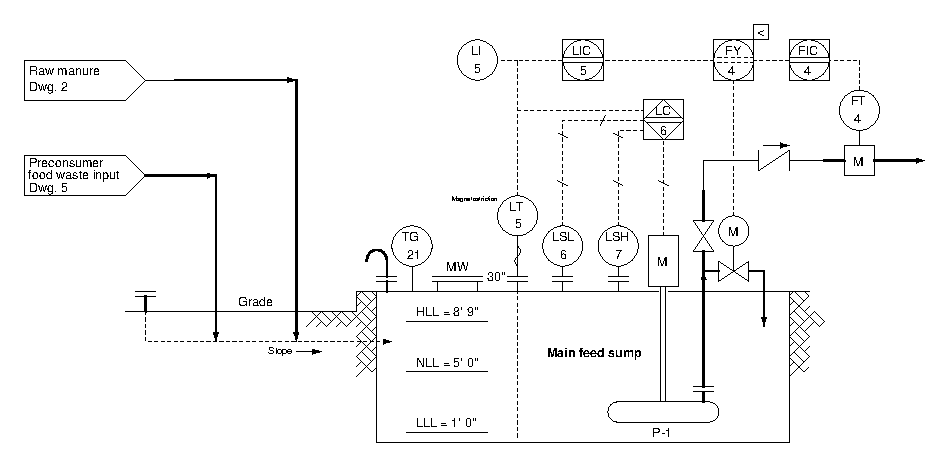
\includegraphics[width=15.5cm]{i00921x05.eps}$$ 













\vfil \eject

\noindent
{\bf Lab questions}

\vskip 20pt

\item{} Sketch connecting wires to make this a working control system.  You should only sketch {\it wires}, as no additional components are necessary:

$$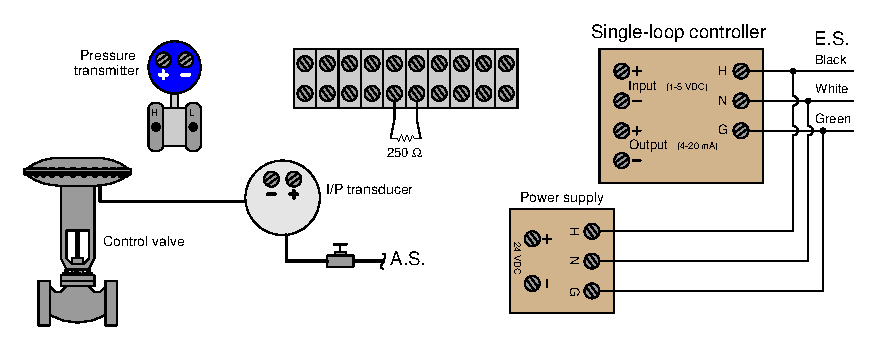
\includegraphics[width=15.5cm]{i00921x07.eps}$$ 

\vskip 20pt

\item{} Identify a practical application for {\it feedforward} control and explain how it works.

\vskip 20pt

\item{} Calculate the pneumatic pressure in a 3-15 PSI range corresponding to 45 percent.

\vskip 20pt

\item{} There is a problem in the control system shown below for the feed sump on an anaerobic digester, which produces methane gas fuel from farm manure and food waste.  The operator reports a low liquid level shown by indicator LI-5 (reading 0 feet 7 inches), and the pump (P-1) not running.  A technician you are working with proposes you take a manual level measurement in the tank using a ``dipstick'' inserted into the sump through a vent pipe to verify the indication shown by LI-5.  Explain what this diagnostic test would tell us about the nature and location of the fault if (1) it did provide a low-level reading in agreement with LI-5, and (2) if it instead showed a normal or high-level reading in disagreement with LI-5.  Be sufficiently detailed in your answer that someone would have a general idea of where the fault was located based on each of your conclusions:

$$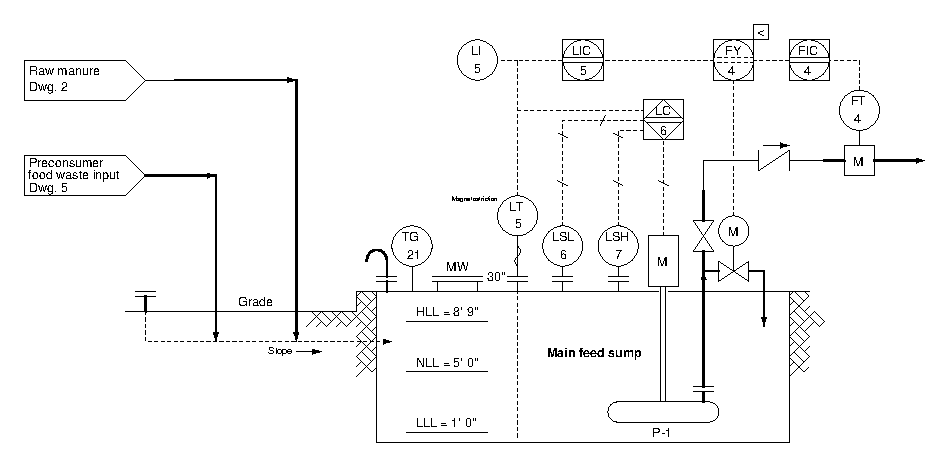
\includegraphics[width=15.5cm]{i00921x05.eps}$$ 

%INDEX% Lab exercise, cascade/ratio/feedforward control strategy

\vfil \eject 



\oppgave{} 
% Copyright 2015, Tony R. Kuphaldt, released under the Creative Commons Attribution License (v 1.0)
% This means you may do almost anything with this work of mine, so long as you give me proper credit

\noindent
{\bf Lab Exercise}

\vskip 5pt

Your primary task is to independently (i.e. no assistance from team members or other classmates) tune multiple control loops, documenting the process open-loop response as well as the process closed-loop responses to both setpoint and load changes.  This documentation must be in the form of computer screen captures, showing the graphic trends of the process as it responds to open-loop and closed-loop tests.  You must do your own loop testing and tuning, the consequence of plagiarism being a failing grade for the course.

Two of the processes you will tune must be {\it real}, working processes.  The last process may be simulated, or it may be another real process with different characteristics than the first two.  All tuning objectives are ``mastery'' -- they must be demonstrated to instructor satisfaction for completion, with no penalty for multiple attempts.

\vskip 10pt

\underbar{Process tuning table:}

% No blank lines allowed between lines of an \halign structure!
% I use comments (%) instead, so that TeX doesn't choke.

$$\vbox{\offinterlineskip
\halign{\strut
\vrule \quad\hfil # \ \hfil & 
\vrule \quad\hfil # \ \hfil & 
\vrule \quad\hfil # \ \hfil & 
\vrule \quad\hfil # \ \hfil \vrule \cr
\noalign{\hrule}
%
% First row
{\bf Performance objective} & {\bf Real \#1} & {\bf Real \#2} & {\bf Real \#3 or Simulated} \cr
%
\noalign{\hrule}
%
% Another row
Description of process &  &  &  \cr
%
\noalign{\hrule}
%
% Another row
Self-reg. {\it vs.} Integ. {\it vs.} Runaway? &  &  &  \cr
%
\noalign{\hrule}
%
% Another row
Measurement of dead time (sec) &  &  &  \cr
%
\noalign{\hrule}
%
% Another row
Measurement of time constant (sec) &  &  &  \cr
%
\noalign{\hrule}
%
% Another row
Measurement of valve stiction (\%) &  &  &  \cr
%
\noalign{\hrule}
%
% Another row
P value after tuning ($K_p$) &  &  &  \cr
%
\noalign{\hrule}
%
% Another row
I value after tuning ($K_i$ or $\tau_i$) &  &  &  \cr
%
\noalign{\hrule}
%
% Another row
D value after tuning ($K_d$ or $\tau_d$) &  &  &  \cr
%
\noalign{\hrule}
%
% Another row
Robust response to SP change? &  &  &  \cr
%
\noalign{\hrule}
%
% Another row
Robust response to load change? &  &  &  \cr
%
\noalign{\hrule}
%
% Another row
{\it Instructor initials} &  &  &  \cr
%
\noalign{\hrule}
%
% Another row
Decommission and lab clean-up &  & -- -- -- -- & -- -- -- -- \cr
%
\noalign{\hrule}
%
% Another row
Team tool locker inspection &  & -- -- -- -- & -- -- -- -- \cr
%
\noalign{\hrule}
} % End of \halign 
}$$ % End of \vbox

In addition to process tuning, you must also troubleshoot a control system and answer lab questions, the same as in regular team-based lab exercises.  A crucial different is that none of the objectives in this entire lab exercise are team-based; rather, all are individual. 

\vskip 10pt

\underbar{Objective completion table:}

% No blank lines allowed between lines of an \halign structure!
% I use comments (%) instead, so that TeX doesn't choke.

$$\vbox{\offinterlineskip
\halign{\strut
\vrule \quad\hfil # \ \hfil & 
\vrule \quad\hfil # \ \hfil \vrule \cr
\noalign{\hrule}
%
% First row
{\bf Performance objective} & pass/score \cr
%
\noalign{\hrule}
%
% Another row
Troubleshooting &   \cr
%
\noalign{\hrule}
%
% Another row
Lab question: Instrument connections &  \cr
%
\noalign{\hrule}
%
% Another row
Lab question: Tuning &  \cr
%
\noalign{\hrule}
%
% Another row
Lab question: Mental math &  \cr
%
\noalign{\hrule}
%
% Another row
Lab question: Diagnostics &  \cr
%
\noalign{\hrule}
} % End of \halign 
}$$ % End of \vbox

\vskip 10pt

The only ``proportional'' scoring in this activity are the lab questions, which are answered by each student individually.  A listing of potential lab questions are shown at the end of this worksheet question.  The lab questions are intended to guide your labwork as much as they are intended to measure your comprehension, and as such the instructor may ask these questions of your team day by day, rather than all at once (on a single day).

When everyone is finished tuning and troubleshooting loops, the last step is to decommission all the working systems as per usual procedure.

\vskip 10pt

{\bf Note: this lab worksheet is your only record of the instructor's validation (signed initials).  Do not lose it, and do not lose your screen-captures of the process responses either!}





\vfil \eject

\noindent
{\bf Lab Exercise -- how to capture ``screen-shots'' on a PC}

\vskip 5pt

An essential part of this lab exercise is capturing graphical trend data from the screen of a personal computer, either running control software (e.g. Emerson DeltaV Operate) or data acquisition software used to monitor process data (e.g. WinDAQ, LabVIEW).  Fortunately, this is really easy to do on any personal computer. 

When you have the screen of the computer displaying what you wish to capture, simply press the ``Print Screen'' key on your keyboard.  This key is usually located to the right of the ``Function'' key row at the top (on a standard desktop keyboard layout -- laptop keyboards are famous for locating seldom-used keys like this in random places).  Pressing the ``Print Screen'' key tells the computer's operating system to copy the entire screen image into a buffer for pasting into any graphics-manipulation or word-processing program you desire.

A utility standard on every Windows operating system is {\it Paint}: a bitmap image creation and manipulation program.  Paint is simple to the point of being crude, but it works just fine for this purpose.  After starting Paint, simply ``Paste'' the captured screen-shot image and save it under any filename you wish.  I strongly recommend using a filename that is unique to you (e.g. {\tt John\_Doe\_process1\_trend2.bmp}).  Remember that you will be capturing multiple screen-shots in this lab exercise, and will need to save every one for presentation to the instructor.  

You may also use Paint (or even a more sophisticated image-manipulation program such as {\it Photoshop} or {\it Gimp}) to add text annotations to your screen-shot images.  For example, some students like to add arrows and lines showing where they measured process gain, or arrows pointing to problems in the trend such as where the control valve sticks.

\vskip 10pt

{\bf Common mistakes:}

\begin{itemize}
\item{} Forgetting to move screenshot files to personal drive, leaving them on the hard drive of the school computer where they may be deleted by other students
\end{itemize}






\vfil \eject

\noindent
{\bf Lab Exercise -- open-loop testing}

\vskip 5pt

Before you can begin to successfully tune a PID-controlled process, you must first understand the characteristics of that process.  A very good way to do this is by performing an {\it open-loop} test: placing the PID controller in manual mode and changing the output value (5\% or so is usually a good amount for the first test) to see what effect this has on the process variable over time.  The PV's response to this ``step-change'' in output can not only reveal the basic characteristics of the process (i.e. self-regulating, integrating, runaway, lag time magnitude, lag order(s), dead time magnitude) but also certain instrument problems (valve stiction, transmitter filtering, etc.).

You should perform several open-loop step-changes to probe the process characteristics: a few in the same direction, then the rest in the other direction.  An analysis of the PV responses following multiple output step-changes will reveal two important characteristics of the process:

\begin{itemize}
\item{} How consistent the process gain is
\item{} Whether the valve has significant hysteresis or stiction (compare opening versus closing)
\end{itemize}

$$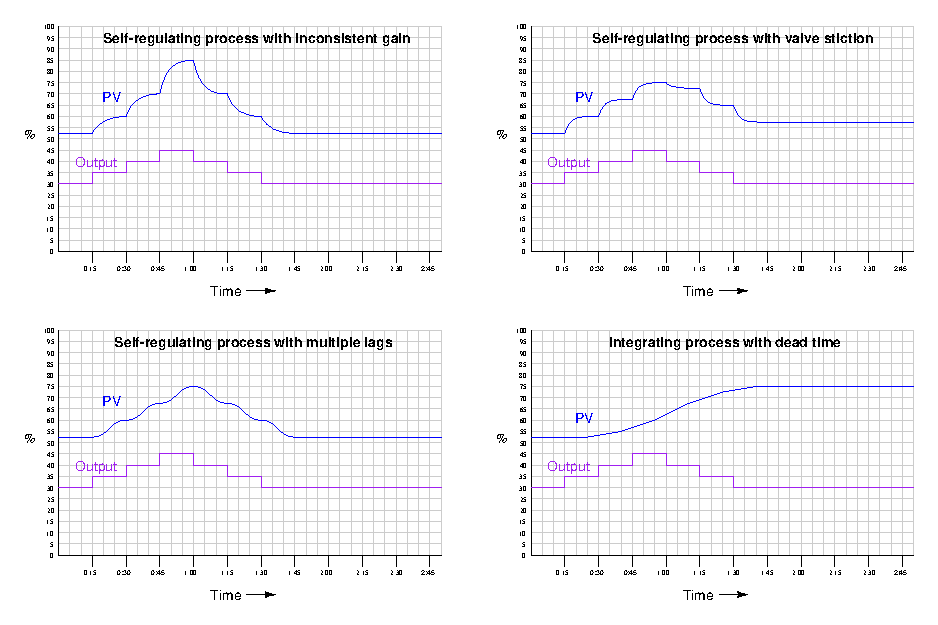
\includegraphics[width=15.5cm]{i01675x02.eps}$$

\vskip 10pt

\filbreak

Valve stiction may be determined by making alternating (up and down) step-changes in manual mode in progressively smaller intervals, noting the largest of those step-changes resulting in no measureable PV change.  The following illustration shows this test applied to a fast, self-regulating process:

$$\includegraphics[width=15.5cm]{i01675x03.eps}$$

\vskip 10pt

{\bf Common mistakes:}

\begin{itemize}
\item{} Trying to probe the process characteristics with the controller in {\it automatic} mode rather than {\it manual} mode
\item{} Making output step-changes that are too large (resulting in PV excursions)
\item{} Not making enough step-changes to fully test process gain consistency or valve stiction
\end{itemize}







\vfil \eject

\noindent
{\bf Lab Exercise -- decide on a tuning strategy}

\vskip 5pt

After you have determined the characteristics of the process and corrected any instrument problems such as transmitter filtering or valve stiction, your next step is to determine how you will tune the PID controller.  Several algorithmic procedures exist, including two methods proposed by Ziegler and Nichols in their 1942 paper, and several more modern methods.  You are free to use whatever tuning method you would like to try, so long as you document the data supporting your tuning decisions (i.e. process characteristics) and also document the trend data showing improvement in process stability as you use your understanding of PID control to fine-tune each process.

Truth be told, many working professionals use algorithmic methods such as Ziegler-Nichols because they really don't understand how PID works, or is supposed to be applied to a real process.  The goal of this lab exercise is to give you plenty of opportunity to try your hand at PID tuning, and to improve upon simple step-by-step methods such as Ziegler-Nichols.  With practice, you will find it possible to make dramatic improvements over ``canned'' PID tuning methods simply by understanding the characteristics of the process and choosing control actions appropriate for those characteristics.

\vskip 10pt

The following table shows several PV responses following a single controller output step-change in manual mode, with suggesting heuristic tuning strategies for each:

$$\includegraphics[width=15.5cm]{i01675x01.eps}$$

Remember that the presence of certain other characteristics in significant amounts (e.g. PV noise, dead time, etc.) also impacts how one should tune a controller. 

\vskip 10pt

{\bf Common mistakes:}

\begin{itemize}
\item{} Making tuning parameter changes that are too large without considering the ill effects those changes might have (e.g. increasing gain by a factor of 10)
\item{} Attempting to ``de-tune'' process or instrument problems that should be repaired (transmitter filtering, valve stiction, etc.)
\end{itemize}









\vfil \eject

\noindent
{\bf Lab Exercise -- robust PID response}

\vskip 5pt

In this exercise you will be asked to demonstrate ``robust'' loop response to both setpoint changes and load changes, which naturally demands a definition for ``robust'' response.  In this context, robust PID response is such that the PV is brought to setpoint as fast as possible, with as little over/undershoot as possible, and absolutely no ``porpoising'' (oscillations prior to reaching setpoint).

\vskip 10pt

A controller that is tuned too ``fast'' will take little time reaching setpoint, but it will do so at the expense of overshooting or undershooting the setpoint value before settling in to the setpoint value.  A controller that is tuned too ``slow'' will not over- or under-shoot setpoint, but will exhibit extended periods of time where the PV is approaching setpoint yet the output value is nowhere near saturation (i.e. the controller is not ``trying'' as hard as it can).

\vskip 10pt

When testing for robust response to load changes, you should introduce load changes in a manner similar to how you introduce setpoint changes: change the load {\it and leave the load in that new state long enough to watch the controller compensate for it.}  A very common error students make when introducing load changes is to do so very briefly, so briefly in fact that the controller never gets a chance to correct for the new load condition.  What you see in such a case is the PV changing due to the load change, and then returning back to setpoint {\it only because the load returned to its previous value, not because the controller actually did anything to make PV return to setpoint!}  So remember, when you introduce load changes, do so the same way you introduce setpoint changes: change the load condition and leave it in that new state, then watch the controller's response to see how quickly the PV returns to the setpoint value, whether there is under- or over-shooting of the setpoint, and/or whether any porpoising occurs.

\vskip 10pt

You will notice that ideal tuning for response to setpoint changes is often different from ideal tuning for response to load changes.  One reason for this is that setpoint changes typically occur more suddenly than load changes.  Another reason is that load changes tend to alter the processes' equilibrium point (i.e. the FCE value necessary to maintain the setpoint) more than setpoint changes.  If you notice a great different between these two responses, you may wish to set the PID algorithm to one where more of the PID equation responds only to changes in {\it PV} and not to changes in {\it error}.

\vskip 10pt

If your controller ``porpoises'' at all, it is detrimental to process control.  ``Porposing'' occurs when either the controller's proportional action or derivative action is too aggressive, causing the controller to over-correct during the PV's approach to setpoint.  Integral is incapable of causing porpoising, because integral action cannot reverse direction unless and until the error changes sign (i.e. until PV crosses setpoint), and porpoising is defined as oscillations occuring {\it prior} to setpoint.  Perhaps the best tool for determining whether excessive gain or excessive derivative action is causing porpoising is to examine the {\it phase shift} between PV and Output during the porpoising period: little or no phase shift reveals excessive P action, while nearly 90$^{o}$ phase shift reveals excessive D action.


\vfil

{\bf Common mistakes:}

\begin{itemize}
\item{} Not properly diagnosing field instrument problems (e.g. sticky valves, over-damped transmitters) prior to tuning.  {\it Pay close attention to your open-loop tests prior to any PID tuning parameter adjustments!!!}
\item{} Relying too much on proportional action (gain) to control fast-acting, self-regulating processes.
\item{} Introducing transient load changes that don't persist long enough to test the controller's ability to correct (i.e. to bring the PV back to SP with different load conditions).
\end{itemize}











\vfil \eject

\noindent
{\bf Lab Exercise -- troubleshooting}

\vskip 5pt

The most challenging aspect of this lab exercise is {\it troubleshooting}, where you demonstrate your ability to logically isolate a problem in the system.  All troubleshooting is done on an individual basis (no team credit!), and must be done {\it on a system you did not help build}, so that you must rely on loop diagrams to find your way around the system instead of from your own memory of building it.

Each student is given a limited amount of time to identify both the general location and nature of the fault, logically justifying all diagnostic steps taken.  All troubleshooting activities will take place under direct instructor supervision to ensure students are working independently and efficiently. 

Failure to correctly identify both the general location and nature of the fault within the allotted time, and/or failing to demonstrate rational diagnostic procedure to the supervising instructor will disqualify the effort, in which case the student must re-try with a different fault.  Multiple re-tries are permitted with no reduction in grade.

A standard multimeter is the only test equipment allowed during the time limit.  No diagnostic circuit breaks are allowed except by instructor permission, and then only after correctly explaining what trouble this could cause in a real system.  

The instructor will review each troubleshooting effort after completion, highlighting good and bad points for the purpose of learning.  Troubleshooting is a skill born of practice and failure, so do not be disappointed in yourself if you must make multiple attempts to pass!  One of the important life-lessons embedded in this activity is how to deal with failure, because it {\it will} eventually happen to you on the job!  There is no dishonor in failing to properly diagnose a fault after doing your level best.  The only dishonor is in taking shortcuts or in giving up.

\vskip 10pt

\filbreak

Recall that every feedback control loop consists of four basic elements: an element that {\it senses} the process variable (e.g. primary sensing element, transmitter), an element that {\it decides} what how to regulate this process variable (e.g. a PID controller), an element that {\it influences} the process variable (e.g. a control valve, motor drive, or some other final control device), and finally the process itself which {\it reacts} to the final control device's actions:

$$ \includegraphics[width=15.5cm]{i01675x05.eps}$$

\noindent
You can check each element of your feedback control loop by comparing its input with its output to see if each element is doing what it should:

\begin{itemize}
\item{$(1)$} \underbar{\bf Decision-making:} Carefully examine the controller faceplate, looking at the values of PV, SP, and Output.  Is the controller taking appropriate action to force PV equal to SP?  In other words, is the Output signal at a value you would expect if the controller were functioning properly to regulate the process variable at setpoint?  If so, then the controller's action and tuning are most likely not at fault.  If not, then the problem definitely lies with the controller.
\item{$(2)$} \underbar{\bf Sensing:} Compare the controller's displayed value for PV with the actual process variable value as indicated by local gauges, by feel, or by any other means of detection.  If there is good correspondence between the controller's PV display and the real process variable, then there probably isn't anything wrong with the measurement portion of the control loop (e.g. transmitter, impulse lines, PV signal wiring, analog input of controller, etc.).  If the displayed PV disagrees with the actual process variable value, then something is definitely wrong here.
\item{$(3)$} \underbar{\bf Influencing:} Compare the controller's displayed value for Output with the actual status of the final control element.  If there is good correspondence between the controller's Output display and the FCE's status, then there probably isn't anything wrong with the output portion of the control loop (e.g. FCE, output signal wiring, analog output of controller, etc.).  If the controller Output value differs from the FCE's state, then something is definitely wrong here.
\item{$(3)$} \underbar{\bf Reacting:} Compare the process variable value with the final control element's state.  Is the process doing what you would expect it to?  If so, the problem is most likely not within the process (e.g. manual valves, relief valves, pumps, compressors, motors, and other process equipment).  If, however, the process is not reacting the way you would expect it to given the final control element's state, then something is definitely awry with the process itself.
\end{itemize}





\vskip 10pt

\filbreak

{\bf Common mistakes:}

\begin{itemize}
\item{} Neglecting to take measurements with your multimeter.
\item{} Neglecting to check other measurements in the system (e.g. pressure gauge readings).
\item{} Incorrectly interpreting the loop diagram (e.g. thinking you're at the wrong place in the system when taking measurements).
\item{} Incorrect multimeter usage (e.g. AC rather than DC, wrong range, wrong test lead placement).  This is especially true when a student comes to lab unprepared and must borrow someone else's meter that is different from theirs!
\end{itemize}

\vskip 10pt

{\bf Remember that the purpose of the troubleshooting exercise is to foster and assess your ability to intelligently diagnose a complex system.  Finding the fault by luck, or by trial-and-error inspection, is not a successful demonstration of skill.  The only thing that counts as competence is your demonstrated ability to logically analyze and isolate the problem, correctly explaining all your steps!}

\vskip 10pt

{\bf Troubleshooting takes a lot of lab time, usually at least two 3-hour lab sessions for everyone in a full class to successfully pass.  Be sure your team budgets for this amount of time as you plan your work, and also be sure to take advantage of your freedom to observe others as they troubleshoot, to better learn this art.}






\vfil \eject

\noindent
{\bf Lab questions}

\vskip 5pt

\begin{itemize}
\item{} {\bf Instrument connections}
\item{} Determine correct wire connections between instruments to create a working 4-20 mA loop circuit, based on diagrams of instruments with terminals labeled
\item{} Correctly determine all electrical sources and loads, as well as all voltage polarities and current directions in a 4-20 mA loop circuit, based on diagrams of instruments with terminals labeled
\end{itemize}

\filbreak

\begin{itemize}
\item{} {\bf Tuning techniques}
\item{} Describe the open-loop method of tuning as designed by Ziegler and Nichols
\item{} Describe the closed-loop (``ultimate'') method of tuning as designed by Ziegler and Nichols
\item{} Identify process types that respond well to aggressive proportional action
\item{} Identify process types that respond poorly to aggressive proportional action
\item{} Identify process types that respond well to aggressive integral (reset) action
\item{} Identify process types that respond poorly to aggressive integral (reset) action
\item{} Identify process types that respond well to aggressive derivative (rate) action
\item{} Identify process types that respond poorly to aggressive derivative (rate) action
\end{itemize}

\filbreak

\begin{itemize}
\item{} {\bf Mental math} (no calculator allowed!)
\item{} Convert a proportional band value into a gain value
\item{} Convert a gain value into a proportional band value
\item{} Convert a repeats/(minute or second) integral value into a (minutes or seconds)/repeat integral value, or vice-versa
\item{} Convert between different pressure units, without relying on the use of a reference for conversion factors (i.e. you must commit the major conversion factors to memory)
\item{} Calculate the pneumatic pressure in a 3-15 PSI range corresponding to $x$ percent.
\item{} Calculate the electrical current in a 4-20 mA range corresponding to $x$ percent.
\item{} Calculate the electrical voltage in a 1-5 volt range corresponding to $x$ percent.
\item{} Calculate the percentage value of a pneumatic pressure signal $x$ PSI in a 3-15 PSI range.
\item{} Calculate the percentage value of an electrical current signal $x$ mA in a 4-20 mA range.
\item{} Calculate the percentage value of an electrical voltage signal $x$ volts in a 1-5 volt range.
\end{itemize}

\filbreak

\begin{itemize}
\item{} {\bf Diagnostics}
\item{} Explain how to distinguish an ``open'' cable fault from a ``shorted'' cable fault using only a voltmeter (no current or resistance measurement, but assuming you are able to break the circuit to perform the test)
\item{} Determine whether or not a given diagnostic test will provide useful information, given a set of symptoms exhibited by a failed system
\item{} Identify at least two plausible faults given the results of a diagnostic test and a set of symptoms exhibited by a failed system
\item{} Propose a diagnostic test for troubleshooting a failed system and then explain the meanings of two different test results
\end{itemize}



\vfil \eject

\noindent
{\bf Lab Exercise -- decommissioning}

\vskip 5pt

The final step of this lab exercise is to decommission your team's entire system and re-stock certain components back to their proper storage locations, the purpose of which being to prepare the lab for the next lab exercise.  Remove your system documentation (e.g. loop diagram) from the common holding area, either discarding it or keeping it for your own records.  Also, remove instrument tag labels (e.g. FT-101) from instruments and from cables.

\vskip 10pt

\indent
{\bf Leave the following components in place, mounted on the racks:}

\begin{itemize}
\item{} Large control valves and positioners
\item{} I/P transducers
\item{} Large electric motors
\item{} Large variable-frequency drive (VFD) units
\item{} Cables inside conduit interconnecting junction boxes together
\item{} Pipe and tube fittings (do not unscrew pipe threads)
\item{} Supply air pressure regulators
\end{itemize}

\vskip 10pt

\indent
{\bf Return the following components to their proper storage locations:}

\begin{itemize}
\item{} Sensing elements (e.g. thermocouples, pH probes, etc.)
\item{} Process transmitters
\item{} ``Jumper'' cables used to connect terminal blocks within a single junction box
\item{} Plastic tubing and tube fittings (disconnect compression-style tube fittings)
\item{} Power cables and extension cords
\item{} Adjustment (loading station) air pressure regulators
\end{itemize}

\vskip 10pt

Finally, you shall return any control system components to their original (factory default) configurations.  This includes controller PID settings, function block programs, input signal ranges, etc.


\underbar{file i01675}
\vskip 10pt \filbreak 





\svar{} 


\vskip 10pt \filbreak 





\notes{} 

{\bf Troubleshooting fault ideas:}

\begin{itemize}
\item{} Connect instrument tubes to wrong port (construction fault)
\item{} Replace I/P restrictor with pre-faulted (plugged) unit (high output fault)
\item{} Replace I/P relay with pre-faulted unit (low or high output fault)
\item{} Turn supply air pressure down well below 15 PSI (low output fault)
\item{} Strip wire at terminal, then insert insulated wire end under terminal and tighten (open wire fault)
\item{} Cut signal cable somewhere in mid-conduit (open wire fault)
\item{} Push a thumbtack through the cable somewhere in mid-conduit (shorted wire fault)
\item{} Wire instrument cable conductors backward (construction fault)
\item{} Plug tube connections using portion of foam earplug stuffed into tube fitting (slow response fault)
\item{} Configure transmitter for excessive damping (slow response fault)
\item{} Configure indicator/controller for excessive damping (slow response fault)
\item{} Mis-configure linear/sq.root characterization of transmitter and/or indicator/controller (nonlinearity fault)
\item{} Miscalibrate transmitter and/or indicator/controller (inaccuracy fault)
\item{} Connect 2.2 k resistor in parallel with 4-20 mA transmitter to simulate partial short in wiring (inaccuracy fault)
\item{} Exchange 250 ohm resistor for a different resistor that looks the same but has the wrong value (inaccuracy fault) 
\item{} Reverse action of controller/positioner/transmitter (wrong response fault)
\item{} Close air supply block valve and leave safety tag hanging on it (operator/technician error)
\item{} Give students wrong loop diagram (documentation fault)
\end{itemize}














\vfil \eject

\noindent
{\bf Lab questions}

\vskip 20pt

\item{$(1)$} Give step-by-step instructions for measuring the amount of {\it dead time} in a control loop.

\vskip 20pt

\item{$(2)$} Consider the water level control system shown below, for a flare gas water seal drum.  Assuming the water level signal (PV) is noise-free, that load changes are small and infrequent, that we don't care how suddenly the control valve may move as it regulates water level, and that the process itself exhibits an {\it integrating} characteristic, predict whether or not the level controller will regulate water level well with:
\begin{itemize}

\item{} Aggressive integral (I) control action: {\it Yes} or {\it No}?

\vskip 20pt

\item{$(3)$} Convert an integral controller setting of 0.5 minutes per repeat into {\it repeats per second}.

\vskip 20pt

\item{$(4)$} Suppose the water seal drum level control system shown below has a problem: LG-5 registers a steady water level of 30\% while LIC-21 registers a steady water level of 50\%.  Local indicator LI-21 also registers a steady water level of 50\%.  The setpoint of LIC-21 is at 50\% and the controller has been in automatic mode the whole time.  Identify one possible fault, as well as one impossible fault, with regard to these symptoms.  Be specific in your identification: both the location (which component) and nature (e.g. open, shorted, plugged) of each fault.

$$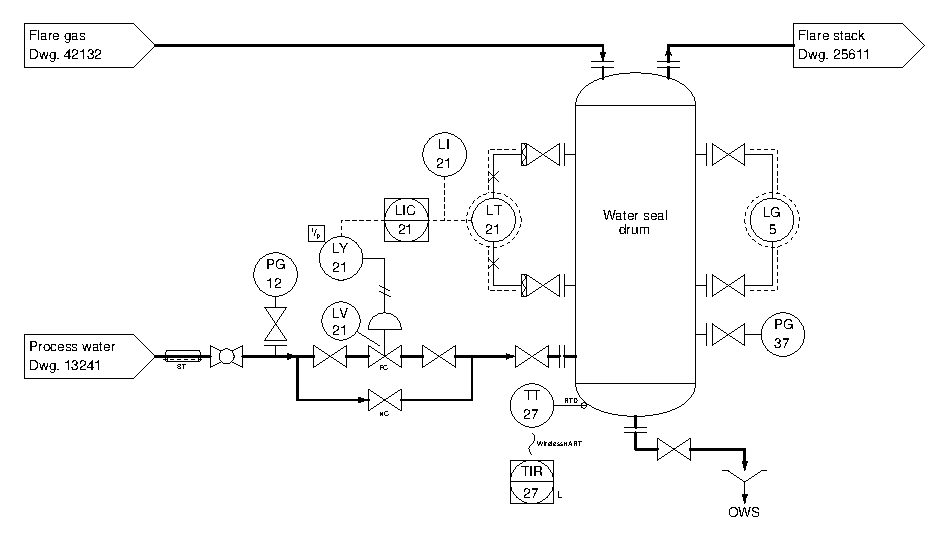
\includegraphics[width=15.5cm]{i01675x04.eps}$$ 

%INDEX% Lab exercise, control loop tuning

\vfil \eject 



\oppgave{} 
% Copyright 2013, Tony R. Kuphaldt, released under the Creative Commons Attribution License (v 1.0)
% This means you may do almost anything with this work of mine, so long as you give me proper credit

\noindent
{\bf Lab Exercise}

\vskip 5pt

Your task is to completely disassemble, reassemble, and bench-set a pneumatically actuated control valve, preferably a Fisher (Emerson) E-body globe valve.  Also, you will build and troubleshoot a control loop to actuate that valve with an electronic 4-20 mA signal, using an I/P transducer as the signal converter between the electronic controller and the pneumatic valve.  

\underbar{Objective completion table:}

% No blank lines allowed between lines of an \halign structure!
% I use comments (%) instead, so that TeX doesn't choke.

$$\vbox{\offinterlineskip
\halign{\strut
\vrule \quad\hfil # \ \hfil & 
\vrule \quad\hfil # \ \hfil & 
\vrule \quad\hfil # \ \hfil & 
\vrule \quad\hfil # \ \hfil & 
\vrule \quad\hfil # \ \hfil & 
\vrule \quad\hfil # \ \hfil & 
\vrule \quad\hfil # \ \hfil \vrule \cr
\noalign{\hrule}
%
% First row
{\bf Performance objective} & {\bf Grading} & {\bf 1} & {\bf 2} & {\bf 3} & {\bf 4} & {\bf Team} \cr
%
\noalign{\hrule}
%
% Another row
Team meeting and prototype sketch & mastery & -- & -- & -- & -- & \cr
%
\noalign{\hrule}
%
% Another row
Control valve disassembly & mastery & -- & -- & -- & -- & \cr
%
\noalign{\hrule}
%
% Another row
Valve component identification & mastery & & & & & -- -- -- -- \cr
%
\noalign{\hrule}
%
% Another row
Torque wrench usage & mastery & & & & & -- -- -- -- \cr
%
\noalign{\hrule}
%
% Another row
Proper stroke length and bench-set & mastery & -- & -- & -- & -- & \cr
%
\noalign{\hrule}
%
% Another row
I/P calibration (with As-Found/As-Left) & mastery & -- & -- & -- & -- &  \cr
%
\noalign{\hrule}
%
% Another row
Circuit design challenge & mastery & & & & & -- -- -- -- \cr
%
\noalign{\hrule}
%
% Another row
Final loop diagram and system inspection & mastery & & & & & -- -- -- -- \cr
%
\noalign{\hrule}
%
% Another row
Demonstration of working system & mastery & -- & -- & -- & -- & \cr
%
\noalign{\hrule}
%
% Another row
Lab question: Instrument connections & proportional &  &  &  &  & -- -- -- -- \cr
%
\noalign{\hrule}
%
% Another row
Lab question: Commissioning & proportional &  &  &  &  & -- -- -- -- \cr
%
\noalign{\hrule}
%
% Another row
Lab question: Mental math & proportional &  &  &  &  & -- -- -- -- \cr
%
\noalign{\hrule}
%
% Another row
Lab question: Diagnostics & proportional &  &  &  &  & -- -- -- -- \cr
%
\noalign{\hrule}
%
% Another row
Lab clean-up & mastery & -- & -- & -- & -- &  \cr
%
\noalign{\hrule}
} % End of \halign 
}$$ % End of \vbox

The only ``proportional'' scoring in this activity are the lab questions, which are answered by each student individually.  A listing of potential lab questions are shown at the end of this worksheet question.  The lab questions are intended to guide your labwork as much as they are intended to measure your comprehension, and as such the instructor may ask these questions of your team day by day, rather than all at once (on a single day).

\vskip 10pt

{\bf It is essential that your team plans ahead what to accomplish each day.  A short (10 minute) team meeting at the beginning of each lab session is a good way to do this, reviewing what's already been done, what's left to do, and what assessments you should be ready for.  There is a lot of work involved with building, documenting, and troubleshooting these working instrument systems!}

As you and your team work on this system, you will invariably encounter problems.  You should always attempt to solve these problems as a team before requesting instructor assistance.  If you still require instructor assistance, write your team's color on the lab whiteboard with a brief description of what you need help on.  The instructor will meet with each team in order they appear on the whiteboard to address these problems.

$$\includegraphics[width=15.5cm]{i00769x01.eps}$$





\vfil \eject

\noindent
{\bf Lab Exercise -- team meeting and prototype sketch}

\vskip 5pt

An important first step in completing this lab exercise is to {\bf meet with your instructor} as a team to discuss safety concerns, team performance, and specific roles for team members.  If you would like to emphasize exposure to certain equipment (e.g. use a particular type of control system, certain power tools), techniques (e.g. fabrication), or tasks to improve your skill set, this is the time to make requests of your team so that your learning during this project will be maximized.

For example, if a team member lacks experience disassembling and reassembling mechanical devices, this lab exercise is an excellent opportunity to gain those skills.  It is {\it strongly} recommended that those team members with the least mechanical experience be the people to disassemble the valve while those with more experience merely supervise.  The team may work together in a more balanced fashion during re-assembly.  

Remember, the purpose of this lab exercise is not to complete it in the least amount of time, but rather for every team member to gain new knowledge and skill.  This is why tasks should not necessarily be assigned with {\it maximum efficiency} in mind as they would at a workplace, but rather with {\it maximum learning} in mind because this is a school.

\vskip 10pt

An absolutely essential step in completing this lab exercise is to work together as a team to {\bf sketch a prototype diagram} showing what you intend to build.  This usually takes the form of a simple electrical schematic and/or loop diagram showing all electrical connections between components, as well as any tubing or piping for fluids.  This prototype sketch need not be exhaustive in detail, but it does need to show enough detail for the instructor to determine if all components will be correctly connected for their safe function.

For example, if you intend to connect field devices to a PLC (Programmable Logic Controller), your prototype sketch must show how those devices will connect to typical input/output terminals on the PLC, where electrical power will be supplied, etc.  Prototype sketches need not show all intermediary connections between components, such as terminal blocks in junction boxes between the field device and the controller.

You should practice good problem-solving techniques when creating your prototype sketch, such as consulting equipment manuals for information on component functions and marking directions of electric current, voltage polarities, and identifying electrical sources/loads.  Use this task as an opportunity to strengthen your analytical skills!  Remember that you will be challenged in this program to do all of this on your own (during ``capstone'' assessments), so do not make the mistake of relying on your teammates to figure this out for you -- instead, treat this as a problem {\it you} must solve and compare your results with those of your teammates.

Your team's prototype sketch is so important that the instructor will demand you provide this plan before any construction on your team's working system begins.  {\it Any team found constructing their system without a verified plan will be ordered to cease construction and not resume until a prototype plan has been drafted and approved!}  Similarly, you should not deviate from the prototype design without instructor approval, to ensure nothing will be done to harm equipment by way of incorrect connections.  Each member on the team should have ready access to this plan (ideally possessing their own copy of the plan) throughout the construction process.  Prototype design sketching is a skill and a habit you should cultivate in school and take with you in your new career.





\vfil \eject

\noindent
{\bf Lab Exercise -- selecting components and planning the system}

\vskip 5pt

One of the most common problems students encounter when building any working system, whether it be a circuit on a solderless breadboard or an instrument loop spanning an entire room, is properly connecting and configuring all components.  An unfortunate tendency among most students is to simply start connecting parts together, essentially designing the system as they go.  This usually leads to improperly-connected components and non-functioning systems, sometimes with the result of destroying components due to those improper connections!

An alternative approach is to plan ahead by designing the system before constructing it.  This is easily done by sketching a diagram showing how all the components should interconnect, then analyzing that diagram and making changes before connecting anything together.  When done as a team, this step ensures everyone is aware of how the system should work, and how it should go together.  The resulting ``prototype'' diagram need not be complex in detail, but it should be detailed enough for anyone to see which component terminals (and ports) connect to terminals and ports of other devices in the system.  For example, your team's prototype sketch should be clear enough to determine all DC electrical components will have the correct polarities.  If your proposed system contains a significant amount of plumbing (pipes and tubes), your prototype sketch should show all those connections as well.

\vskip 10pt

Your first step should be identifying the model of control valve assigned to you, then finding appropriate documentation for it.  The Emerson website contains manuals for all the Fisher valves they sell, so your best resource is the Internet (and/or your Instrumentation Reference where a variety of instrument manuals have been downloaded for you).  Use this documentation to locate diagrams of the valve assembly as well as instructions.  Your instructor will check to see you have located and are familiar with the equipment manual(s).

\vskip 10pt

Your team's prototype sketch is so important that the instructor will demand you provide this plan before any construction on your team's working system begins.  {\it Any team found constructing their system without a verified plan will be ordered to cease construction and not resume until a prototype plan has been drafted and approved!}  Each member on the team should have ready access to this plan (ideally possessing their own copy of the plan) throughout the construction process.  Prototype design sketching is a skill and a habit you should cultivate in school and take with you in your new career.

\vskip 10pt

{\bf Planning a functioning system should take no more than an hour if the team is working efficiently, and will save you hours of frustration (and possible component destruction!).}





\vfil \eject

\noindent
{\bf Lab Exercise -- disassembling and re-assembling the valve}

\vskip 5pt

The {\it Lessons In Industrial Instrumentation} textbook has an Appendix section documenting the complete tear-down of a Fisher ``E-body'' sliding-stem globe valve.  You may want to use this as a guide in the disassembly of your team's valve.  Feel free to take your own digital photographs as you disassemble the valve, to better aid in your understanding of its function and to serve as a re-assembly guide.

A safety tip for disassembly is to make releasing spring tension your {\it first} step.  Back off the spring adjuster until it spins loosely, and then there should be no stored energy in the actuator spring to hurt you during disassembly.  If ever you are loosening a nut or bolt on the valve assembly and it seems to be ``stiff'' during most of the loosening process, you may very well have stored spring tension inside the valve that should be relieved before any further loosening is attempted.

You and your teammates should disassemble the control valve down to the last nut and bolt.  Use a coffee can or other container to place small items such as nuts, bolts, screws, brackets, clips, and O-rings.  Use a larger bucket or tub to hold major valve components during the disassembly and re-assembly processes.

\vskip 10pt

After disassembling the valve, each team member must properly identify a few key components of the valve (and their functions) as prompted by the instructor.

\vskip 10pt

When all team members have successfully passed the component identification test, the team is cleared to re-assemble the valve.  Be careful when doing so -- if components don't seem to fit smoothly, and/or require substantial force to put together, you are likely doing something incorrect.  Stop and re-evaluate your actions before you break something!

A helpful precaution to take when reassembling the valve body is to periodically move the valve stem by hand to ensure it continues to more freely and with full stroke (the stem should actually move just a bit {\it farther} than the rated stroke length, so long as the actuator remains unattached).  If the stem exhibits any sign of limited travel or binding, it is a sign something is wrong with the assembly, and you should disassemble it again to check your work.

Be sure to {\it cross-torque} all nuts and bolts arranged in a circular pattern (e.g. nuts on bonnet studs, diaphragm casing nuts and bolts): this means alternating sides when choosing the next nut/bolt to tighten.  Use a torque wrench to apply the amount of torque specified in the manufacturer's instruction manual, individually demonstrating this tool usage to the instructor.  Proper execution of the torque sequence will ensure the assembly will not be warped by uneven bolt stress.

\vskip 10pt

{\bf Common mistakes:}

\begin{itemize}
\item{} The most-mechanically-minded students doing all the work, when they should let their lesser-mechanically-inclined teammates do most of the disassembly.
\item{} Failing to consult documentation, especially with regard to the proper assembly of the stem packing.
\item{} Not organizing parts in containers.
\item{} Trying to hoist heavy valve components by yourself -- improper lifting techniques and lack of teamwork.
\item{} Using tools improperly: e.g. using adjustable wrenches when combination wrenches will do, using slip-joint and tongue-and-groove pliers instead of wrenches, using metal tools (hammer heads) to tap metal components out of place instead of softer tools such as the wooden handle of a hammer.
\item{} Not checking valve stem stroke periodically while reassembling valve body.
\end{itemize}

\vskip 10pt

{\bf Thoroughly disassembling a control valve should take no more than one full lab session (3 hours) if the team is working efficiently!  Identifying components and re-assembling the control valve may take more than one whole (3 hour) lab session.}


\vfil \eject

\noindent
{\bf Lab Exercise -- setting stroke length and bench-set pressure}

\vskip 5pt

The most complex step in the re-assembly process is properly setting both the stem stroke length and the bench-set pressure.  This step takes a bit of time to do, and it is easy to mis-understand, so be sure to budget plenty of time (at least an hour or two) to do it right.  Be sure to involve all team members in this procedure, as it is easy to mis-understand.

In a sliding-stem control valve, the length of the valve stem's travel (``stroke'') is determined by the coupling of the valve and actuator stems.  A {\it stem connector} couples these two stems together at just the right total stem length so that the valve plug ``bottoms out'' on the seat when at the 0\% position and the actuator ``tops out'' on the upper casing at the 100\% position.  In order to set the proper coupling point between the two stems, you will need some way to apply variable air pressures to the diaphragm actuator to move it between its extreme positions.  A small air pressure regulator connected to a compressed air supply works well for this purpose, and need not be precision.

\vskip 10pt

Consult the manufacturer's manual for your control valve's actuator to obtain step-by-step instructions for setting the valve spring tension (``bench set'') and also properly installing the stem connector (coupling).  The result, after correctly following the procedures, is that the valve's stem travel should exactly match what is shown on the travel indicator scale.  Your instructor will judge your team's proper assembly as such: the valve stem should just begin to move at slightly above the lower bench-set pressure, and reach full stroke just shy of the upper bench-set pressure value.  Decreasing the applied air pressure below the lower bench-set value or increasing the pressure above the upper bench-set value should produce no stem motion at all (i.e. the valve should mechanically ``bottom out'' and ``top out'' at these bench-set pressure values).

\vskip 10pt

Stroke length and bench-set are both crucial parameters for efficient and safe control valve operation.  Wrong stroke length can prevent the valve from fully opening (if the stems are coupled too far apart) and may even prevent it from fully closing (if the stems are coupled much too close together).  Proper stroke length ensures the valve will exhibit the engineered flow characteristics throughout its range of movement.  Improper bench set may result in insufficient seating pressure (if spring tension is too weak), causing the valve to pass fluid by when it should be fully closed.

\vskip 10pt

{\bf Common mistakes:}

\begin{itemize}
\item{} Not following the manufacturer's instructions {\it precisely}.
\end{itemize}






\vfil \eject

\noindent
{\bf Lab Exercise -- circuit design challenge}

\vskip 5pt

Connect an ``ice-cube'' relay to a low-voltage DC source as well as 120 volts AC so that a hand-operated switch will control the energization of a 120 VAC load.  All electrical connections must be made using a terminal strip (no twisted wires, crimp splices, wire nuts, spring clips, or ``alligator'' clips permitted), and the 120 VAC portion of the circuit must be fused for overcurrent protection.

This exercise tests your ability to properly interpret the ``pinout'' of an electromechanical relay, properly wire a switch to control a relay's coil, properly wire a load to the contacts of a relay, properly select NO/NC contacts on both the switch and the relay, and use a terminal strip to organize all electrical connections.

$$\includegraphics[width=15.5cm]{i00769x03.eps}$$

\vskip 10pt

The following components and materials will be available to you: assorted ``ice cube'' {\bf relays} with DC-rated coils and matching {\bf sockets} ; assorted pushbutton {\bf switches} ; {\bf terminal strips} ; lengths of {\bf hook-up wire} ; {\bf battery clips} (holders) ; 120 VAC {\bf power cord} with {\bf fuse assembly} ; 120 VAC {\bf lamp or other suitable load}.

\vskip 10pt

You will be expected to supply your own screwdrivers and multimeter for assembling and testing the circuit at your desk.  The instructor will supply the battery(ies) to power your circuit when you are ready to see if it works.  Until that time, your circuit will remain unpowered.

\vskip 20pt

\noindent
{\bf Load/switch status} (instructor chooses): \hskip 20pt \underbar{\hskip 20pt} On when pressed \hskip 10pt {\it or} \hskip 10pt \underbar{\hskip 20pt} Off when pressed

\vfil

Study reference: the ``Control Relays'' section of {\it Lessons In Industrial Instrumentation}.







\vfil \eject

\noindent
{\bf Lab Exercise -- building the system}

\vskip 5pt

The Instrumentation lab is set up to facilitate the construction of working instrument ``loops,'' with over a dozen junction boxes, pre-pulled signal cables, and ``racks'' set up with 2-inch vertical pipes for mounting instruments.  The only wires you should need to install to build a working system are those connecting the field instrument to the nearest junction box, and then small ``jumper'' cables connecting different pre-installed cables together within intermediate junction boxes.

After getting your prototype sketch approved by the instructor, you are cleared to build a hand-control system for it.  This will consist of a loop controller placed into ``manual'' mode to allow direct control over the valve's position.  There will be no transmitter installed in this loop -- just the valve and the I/P converter necessary to convert the controller's 4-20 mA output signal into a pneumatic signal to move the valve.  Feel free to use 1/4 inch plastic tubing for all pneumatic signal connections, and be sure not to exceed the rated supply pressure for the I/P (as documented in the I/P manual).

Your hand-control system needs to have a loop number, so all instruments within it may be properly labeled.  This loop number needs to be unique, so that another team does not label their instruments and tubes the same as yours.  One way to make your loop number unique is to use the equivalent resistor color-code value for your team's color in the loop number.  For example, if you are the ``Red'' team, your loop number could be ``2''. 

The controller itself should be labeled ``HC-'' because it is a ``hand'' controller, allowing a human operator manual control over the valve's position.

\vskip 10pt

{\bf Common mistakes:}

\begin{itemize}
\item{} Neglecting to consult the manufacturer's documentation for the I/P converter (e.g. how to connect pneumatic signal lines, how to calibrate it).
\item{} Improper pipe/tube fitting installation (e.g. trying to thread tube fittings into pipe fittings and vice-versa).
\item{} Over-tightening tube fittings (remember, no more than 1-1/4 turns when assembling, and no more than ``snug'' when re-making the connection!).
\item{} Students working on portions of the system in isolation, not sharing with their teammates what they did and how.  It is important that the whole team learns all aspects of their system!
\end{itemize}


\vfil \eject

\noindent
{\bf Lab Exercise -- documenting the system}

\vskip 5pt

Each student must sketch their own {\it loop diagram} for their team's system, following proper ISA conventions.  Sample loop diagrams are shown in the next question in this worksheet.  These loop diagrams must be {\it comprehensive} and {\it detailed}, showing every tube connection, every tube, range points, etc.  The principle to keep in mind here is to make the loop diagram so complete and unambiguous that anyone can follow it to see what connects to what, even someone unfamiliar with industrial instrumentation.  In industry, loops are often constructed by contract personnel with limited understanding of how the system is supposed to function.  The loop diagrams they follow must be so complete that they will be able to connect everything properly without necessarily understanding how it is supposed to work.

Every instrument and every signal tube in your loop needs to be properly labeled with an ISA-standard tag number.  An easy way to do this is to wrap a short piece of masking tape around each tube (and placed on each instrument) then writing on that masking tape with a permanent marker.  Although no industry standard exists for labeling signal tubes, a good recommendation is to label each tube with the tag number of the field instrument it goes to.  Thus, every length of tube in a hand control loop should be labeled ``HV-$x$'' (where ``$x$'' is the loop number).

When your entire team is finished drafting your individual loop diagrams, call the instructor to do an inspection of the loop.  Here, the instructor will have students take turns going through the entire loop, with the other students checking their diagrams for errors and omissions along the way.  During this time the instructor will also inspect the quality of the installation, identifying problems such as frayed wires, improperly crimped terminals, poor cable routing, missing labels, lack of wire duct covers, etc.  The team must correct all identified errors in order to receive credit for their system.  

After successfully passing the inspection, each team member needs to place their loop diagram in the diagram holder located in the middle of the lab behind the main control panel.  When it comes time to troubleshoot another team's system, this is where you will go to find a loop diagram for that system!

\vskip 10pt

{\bf Common mistakes:}

\begin{itemize}
\item{} Forgetting to label all signal tubes (see example loop diagrams).
\item{} Forgetting to label all field instruments with their own tag names (e.g. HY-83 for the I/P transducer).
\item{} Forgetting to put your name on the loop diagram!
\item{} Basing your diagram off of a team-mate's diagram, rather than closely inspecting the system for yourself.
\item{} Not placing loop sheet instruments in the correct orientation (field instruments on the left, control room instruments on the right).
\end{itemize}

\vskip 10pt

{\bf Creating and inspecting accurate loop diagrams should take no more than one full lab session (3 hours) if the team is working efficiently!}





\vfil \eject

\noindent
{\bf Lab Exercise -- I/P calibration}

\vskip 5pt

Each team must calibrate their I/P transducer for a range appropriate to their control valve's actuator pressure range (usually 3-15 PSI).  As in all cases where an instrument must be calibrated, you will need to check the instrument's response against one or more {\it standards}.  In this case, the ideal standard to use for measuring the I/P output pressure is a {\it test gauge}, and the ideal standard to use for establishing the 4-20 mA current signal into the I/P is a {\it loop calibrator} set to ``source'' current.

$$\includegraphics[width=15.5cm]{i00769x02.eps}$$

Read the manufacturer's documentation on the I/P transducer for details on how to calibrate it.  Like an analog measuring instrument, the procedure will involve trial-and-error applications of LRV and URV input signal values, adjusting the ``zero'' and ``span'' screws of the I/P until it tracks accurately at those two points.  Note that the zero and span screw adjustments on most I/P converters are interactive: adjusting the span will affect the zero, necessitating a lot of back-and-forth applications of LRV and URV, zero screw turning and span screw turning.

\filbreak

Document the accuracy of your I/P's calibration before and after adjustment in these tables, at five different points throughout its sensing range.  The ``Applied'' current is the amount of electric current you apply to the I/P's input using a loop calibrator, and the ``Output'' signal is the amount of air pressure output by the I/P (the 3-15 PSI range):

\vskip 10pt

{\bf As-Found calibration table}

% No blank lines allowed between lines of an \halign structure!
% I use comments (%) instead, so that TeX doesn't choke.

$$\vbox{\offinterlineskip
\halign{\strut
\vrule \quad\hfil # \ \hfil & 
\vrule \quad\hfil # \ \hfil & 
\vrule \quad\hfil # \ \hfil & 
\vrule \quad\hfil # \ \hfil \vrule \cr
\noalign{\hrule}
%
% First row
Applied pressure & Output signal (actual) & Output signal (ideal) & Error (\% of span) \cr
%
\noalign{\hrule}
%
% Another row
 &  &  & \cr
%
\noalign{\hrule}
%
% Another row
 &  &  & \cr
%
\noalign{\hrule}
%
% Another row
 &  &  & \cr
%
\noalign{\hrule}
%
% Another row
 &  &  & \cr
%
\noalign{\hrule}
%
% Another row
 &  &  & \cr
%
\noalign{\hrule}
} % End of \halign 
}$$ % End of \vbox

\vskip 10pt

{\bf As-Left calibration table}

% No blank lines allowed between lines of an \halign structure!
% I use comments (%) instead, so that TeX doesn't choke.

$$\vbox{\offinterlineskip
\halign{\strut
\vrule \quad\hfil # \ \hfil & 
\vrule \quad\hfil # \ \hfil & 
\vrule \quad\hfil # \ \hfil & 
\vrule \quad\hfil # \ \hfil \vrule \cr
\noalign{\hrule}
%
% First row
Applied pressure & Output signal (actual) & Output signal (ideal) & Error (\% of span) \cr
%
\noalign{\hrule}
%
% Another row
 &  &  & \cr
%
\noalign{\hrule}
%
% Another row
 &  &  & \cr
%
\noalign{\hrule}
%
% Another row
 &  &  & \cr
%
\noalign{\hrule}
%
% Another row
 &  &  & \cr
%
\noalign{\hrule}
%
% Another row
 &  &  & \cr
%
\noalign{\hrule}
} % End of \halign 
}$$ % End of \vbox

When finished calibrating your I/P converter, be sure to place a calibration tag on it showing the range and the date it was calibrated.  The first page of this lab exercise has cut-out calibration tags you may tape to the I/P for this purpose.

The accuracy of your calibration will be checked by the instructor while installed in the loop, setting the hand controller's output to various levels and checking the valve stem position for correspondence.  It should be noted that I/P transducers are not typically ``precision'' instruments like process transmitters, and as such you may find substantial variations in calibration resulting from modest changes in supply air pressure and/or mounting position.

\vskip 10pt

{\bf Common mistakes:}

\begin{itemize}
\item{} Applying excessive force to I/P adjustments.  This is a delicate mechanism!  As such, it should {\it not} require forceful adjustment!!  If you have to {\it force} something, you're probably doing it wrong.
\item{} Improper supply air pressure to the converter (see the manual for supply air pressure specifications)
\item{} Improper pipe/tube fitting installation (e.g. trying to thread tube fittings into pipe fittings and vice-versa).
\item{} Neglecting to place a calibration tag on the I/P converter after calibrating it.
\end{itemize}








\vskip 10pt

\vfil \eject

\noindent
{\bf Lab questions}

\begin{itemize}
\item{} {\bf Instrument connections}
\item{} Determine correct wire connections between instruments to create a working 4-20 mA loop circuit, based on diagrams of instruments with terminals labeled
\item{} Correctly determine all electrical sources and loads, as well as all voltage polarities and current directions in a 4-20 mA loop circuit, based on diagrams of instruments with terminals labeled
\end{itemize}

\filbreak

\begin{itemize}
\item{} {\bf Commissioning and Documentation}
\item{} Identify alternative valve actuators (other than pneumatic diaphragm)
\item{} Identify the major components of a rotary ball control valve from a diagram
\item{} Explain the function of valve stem packing, and how to change it
\item{} Explain how to adjust the compression on a valve's stem packing
\item{} Explain how to properly set valve stroke length and bench-set pressure
\item{} Explain the significance of properly setting valve stroke length and bench-set pressure
\end{itemize}

\filbreak

\begin{itemize}
\item{} {\bf Mental math} (no calculator allowed!)
\item{} Convert between different pressure units, without relying on the use of a reference for conversion factors (i.e. you must commit the major conversion factors to memory)
\item{} Calculate the correct pneumatic output pressure (PSI) from an I/P transducer given an applied current (mA) signal input and a specified range (e.g. 4-20 mA input ; 3-15 PSI output)
\item{} Calculate the applied input current (mA) to an I/P transducer given a measured pneumatic output pressure (PSI) and a specified range (e.g. 4-20 mA input ; 3-15 PSI output) 
\item{} Calculate the percentage of span error for an I/P transducer given a calibration range and an As-Found calibration table 
\item{} Calculate force generated by a diaphragm or piston actuator given diameter and applied fluid pressure in units of PSI
\end{itemize}

\filbreak

\begin{itemize}
\item{} {\bf Diagnostics}
\item{} Determine whether or not a given diagnostic test will provide useful information, given a set of symptoms exhibited by a failed system
\item{} Identify at least two plausible faults given the results of a diagnostic test and a set of symptoms exhibited by a failed system
\item{} Propose a diagnostic test for troubleshooting a failed system and then explain the meanings of two different test results
\end{itemize}



\vfil \eject

\noindent
{\bf Lab Exercise -- decommissioning and clean-up}

\vskip 5pt

The final step of this lab exercise is to decommission your team's entire system and re-stock certain components back to their proper storage locations, the purpose of which being to prepare the lab for the next lab exercise.  Remove your system documentation (e.g. loop diagram) from the common holding area, either discarding it or keeping it for your own records.  Also, remove instrument tag labels (e.g. FT-101) from instruments and from cables.  Perform general clean-up of your lab space, disposing of all trash, placing all tools back in their proper storage locations, sweeping up bits of wire off the floor and out of junction boxes, etc.

\vskip 10pt

\indent
{\bf Leave the following components in place, mounted on the racks:}

\begin{itemize}
\item{} Large control valves and positioners
\item{} I/P transducers
\item{} Large electric motors
\item{} Large variable-frequency drive (VFD) units
\item{} Cables inside conduit interconnecting junction boxes together
\item{} Pipe and tube fittings (do not unscrew pipe threads)
\item{} Supply air pressure regulators
\end{itemize}

\vskip 10pt

\indent
{\bf Return the following components to their proper storage locations:}

\begin{itemize}
\item{} Sensing elements (e.g. thermocouples, pH probes, etc.)
\item{} Process transmitters
\item{} ``Jumper'' cables used to connect terminal blocks within a single junction box
\item{} Plastic tubing and tube fittings (disconnect compression-style tube fittings)
\item{} Power cables and extension cords
\item{} Adjustment (loading station) air pressure regulators
\end{itemize}

\vskip 10pt

Finally, you shall return any control system components to their original (factory default) configurations.  This includes controller PID settings, function block programs, input signal ranges, etc.



\underbar{file i00769}
\vskip 10pt \filbreak 





\svar{} 


\vskip 10pt \filbreak 





\notes{} 

\noindent
{\bf Loop diagrams / inspections:}

I strongly recommend checking off students' loop diagrams while you inspect their loop (checking for secure wiring, proper tubing, good conduit installation, etc.) with them.  Have all team members take you on a ``tour'' of their completed loop, with each team member explaining a different portion of the loop you select while using their own loop diagram as a guide.  While a student is explaining their section of the loop, you can check the other students' loop diagrams for accuracy.  This not only saves time by consolidating the tasks of loop inspection and loop diagram verification, but it also ensures students can actually relate their loop diagrams to the loop they have built and articulate that understanding to you.

\vskip 10pt

\goodbreak

{\bf Troubleshooting fault ideas:}

\begin{itemize}
\goodbreak
\item{} Connect instrument tubes to wrong port (construction fault)
\item{} Replace I/P restrictor with pre-faulted (plugged) unit (high output fault)
\item{} Replace I/P relay with pre-faulted unit (low or high output fault)
\item{} Turn supply air pressure down well below 15 PSI (low output fault)
\item{} Strip wire at terminal, then insert insulated wire end under terminal and tighten (open wire fault)
\item{} Cut signal cable somewhere in mid-conduit (open wire fault)
\item{} Push a thumbtack through the cable somewhere in mid-conduit (shorted wire fault)
\item{} Wire instrument cable conductors backward (construction fault)
\item{} Plug tube connections using portion of foam earplug stuffed into tube fitting (slow response fault)
\item{} Close air supply block valve and leave safety tag hanging on it (operator/technician error)
\item{} Give students wrong loop diagram (documentation fault)
\end{itemize}















\vfil \eject

\noindent
{\bf Lab questions}

\vskip 20pt

\item{$(1)$} Sketch the necessary wire connections allowing the loop calibrator to exert control over the valve in this diagram, and also identify the proper mode ({\it Read}, {\it Source}, or {\it Simulate}) to set the calibrator:

$$\includegraphics[width=15.5cm]{i00769x05.eps}$$

\vskip 40pt

\item{$(2)$} Describe the proper precedure for setting both valve stroke length and bench-set pressure on a sliding-stem control valve.

\vskip 20pt

\filbreak

\item{$(3)$} Calculate the amount of force generated by a 14 inch diameter valve actuator diaphragm, with an applied air pressure of 30 PSI.

\vskip 40pt

\item{$(4)$} Control valve TV-37 has failed in the closed position and refuses to open.  A voltmeter reading between terminals 3 and 4 shows 3.5 volts.  Identify one possible fault, as well as one impossible fault, with regard to these symptoms.  Be specific in your identification: both the location (which component) and nature (e.g. open, shorted, plugged) of each fault.

$$\includegraphics[width=15.5cm]{i00769x04.eps}$$















\vfil \eject

\noindent
{\bf Lab questions}

\vskip 20pt

\item{$(1)$} Sketch the necessary wire connections allowing the Honeywell controller to exert manual control over the valve in this diagram:

$$\includegraphics[width=15.5cm]{i00769x05.eps}$$

\vskip 40pt

\item{$(2)$} Explain the significance of properly setting valve stroke length and bench-set pressure on a sliding-stem control valve.

\vskip 20pt

\filbreak

\item{$(3)$} Calculate the percentage of span error for an I/P transducer given a calibrated range of 3-15 PSI, if we know it outputs 11.85 PSI of air pressure at an input current of 16.00 mA.

\vskip 40pt

\item{$(4)$} Control valve TV-37 has failed in the wide-open position and refuses to close at all.  A voltmeter reading between terminals 3 and 4 shows 0.8 volts.  Identify one possible fault, as well as one impossible fault, with regard to these symptoms.  Be specific in your identification: both the location (which component) and nature (e.g. open, shorted, plugged) of each fault.

$$\includegraphics[width=15.5cm]{i00769x04.eps}$$




%INDEX% Lab exercise, control valve rebuild

\vfil \eject 



\oppgave{} 
% Copyright 2015, Tony R. Kuphaldt, released under the Creative Commons Attribution License (v 1.0)
% This means you may do almost anything with this work of mine, so long as you give me proper credit

\noindent
{\bf Lab Exercise -- introduction}

\vskip 5pt

Your task is to build, document, and troubleshoot a telemetry system consisting of an analog sensor connected to a data acquisition (DAQ) module, which then sends the data over Ethernet to a personal computer.  Temperature and pressure are suggested process variables to measure.  Electric current (measured using a shunt resistor or a current transformer) is another excellent process variable to measure, and this works well to introduce the specialized topic of electric power metering and protection.  In fact, setting up an electronic protective relay to sense AC current and initiate a breaker ``trip'' signal is an excellent alternative to using a generic DAQ.  Other process variables are open for consideration, though.

The following table of objectives show what you and your team must complete within the scheduled time for this lab exercise.  Note how some of these objectives are individual, while others are for the team as a whole:

\underbar{Objective completion table:}

% No blank lines allowed between lines of an \halign structure!
% I use comments (%) instead, so that TeX doesn't choke.

$$\vbox{\offinterlineskip
\halign{\strut
\vrule \quad\hfil # \ \hfil & 
\vrule \quad\hfil # \ \hfil & 
\vrule \quad\hfil # \ \hfil & 
\vrule \quad\hfil # \ \hfil & 
\vrule \quad\hfil # \ \hfil & 
\vrule \quad\hfil # \ \hfil & 
\vrule \quad\hfil # \ \hfil \vrule \cr
\noalign{\hrule}
%
% First row
{\bf Performance objective} & {\bf Grading} & {\bf 1} & {\bf 2} & {\bf 3} & {\bf 4} & {\bf Team} \cr
%
\noalign{\hrule}
%
% Another row
Team meeting and prototype sketch (do {\it first!}) & mastery & -- & -- & -- & -- & \cr
%
\noalign{\hrule}
%
% Another row
Circuit design challenge & mastery & & & & & -- -- -- -- \cr
%
\noalign{\hrule}
%
% Another row
Final documentation and system inspection & mastery & & & & & -- -- -- -- \cr
%
\noalign{\hrule}
%
% Another row
Demonstrate IP ``ping'' utility & mastery & -- & -- & -- & -- &  \cr
%
\noalign{\hrule}
%
% Another row
Demonstrate use of a ``knockout punch'' tool & mastery & -- & -- & -- & -- &  \cr
%
\noalign{\hrule}
%
% Another row
Accurate measurement of variable ($\pm$ 1\% of span) & mastery & -- & -- & -- & -- &  \cr
%
\noalign{\hrule}
%
% Another row
Data communicated via Ethernet & mastery & -- & -- & -- & -- &  \cr
%
\noalign{\hrule}
%
% Another row
Troubleshooting & mastery & & & & & -- -- -- -- \cr
%
\noalign{\hrule}
%
% Another row
Lab question: Instrument connections & proportional &  &  &  &  & -- -- -- -- \cr
%
\noalign{\hrule}
%
% Another row
Lab question: Commissioning & proportional &  &  &  &  & -- -- -- -- \cr
%
\noalign{\hrule}
%
% Another row
Lab question: Mental math & proportional &  &  &  &  & -- -- -- -- \cr
%
\noalign{\hrule}
%
% Another row
Lab question: Diagnostics & proportional &  &  &  &  & -- -- -- -- \cr
%
\noalign{\hrule}
%
% Another row
Decommission and lab clean-up & mastery & -- & -- & -- & -- &  \cr
%
\noalign{\hrule}
} % End of \halign 
}$$ % End of \vbox

The only ``proportional'' scoring in this activity are the lab questions, which are answered by each student individually.  A listing of potential lab questions are shown at the end of this worksheet question.  The lab questions are intended to guide your labwork as much as they are intended to measure your comprehension, and as such the instructor may ask these questions of your team day by day, rather than all at once (on a single day).

\vskip 10pt

{\bf It is essential that your team plans ahead what to accomplish each day.  A short (10 minute) team meeting at the beginning of each lab session is a good way to do this, reviewing what's already been done, what's left to do, and what assessments you should be ready for.  There is a lot of work involved with building, documenting, and troubleshooting these working instrument systems!}

As you and your team work on this system, you will invariably encounter problems.  You should always attempt to solve these problems as a team before requesting instructor assistance.  If you still require instructor assistance, write your team's color on the lab whiteboard with a brief description of what you need help on.  The instructor will meet with each team in order they appear on the whiteboard to address these problems.




\vfil \eject

\noindent
{\bf Lab Exercise -- team meeting, prototype sketch, and instrument selection}

\vskip 5pt

An important first step in completing this lab exercise is to {\bf meet with your instructor} as a team to discuss safety concerns, team performance, and specific roles for team members.  If you would like to emphasize exposure to certain equipment (e.g. use a particular type of control system, certain power tools), techniques (e.g. fabrication), or tasks to improve your skill set, this is the time to make requests of your team so that your learning during this project will be maximized.

\vskip 10pt

An absolutely essential step in completing this lab exercise is to work together as a team to {\bf sketch a prototype diagram} showing what you intend to build.  This usually takes the form of a simple electrical schematic and/or loop diagram showing all electrical connections between components, as well as any tubing or piping for fluids.  This prototype sketch need not be exhaustive in detail, but it does need to show enough detail for the instructor to determine if all components will be correctly connected for their safe function.

For example, if you intend to connect field devices to a PLC (Programmable Logic Controller), your prototype sketch must show how those devices will connect to typical input/output terminals on the PLC, where electrical power will be supplied, etc.  Prototype sketches need not show all intermediary connections between components, such as terminal blocks in junction boxes between the field device and the controller.

You should practice good problem-solving techniques when creating your prototype sketch, such as consulting equipment manuals for information on component functions and marking directions of electric current, voltage polarities, and identifying electrical sources/loads.  Use this task as an opportunity to strengthen your analytical skills!  Remember that you will be challenged in this program to do all of this on your own (during ``capstone'' assessments), so do not make the mistake of relying on your teammates to figure this out for you -- instead, treat this as a problem {\it you} must solve and compare your results with those of your teammates.

Your team's prototype sketch is so important that the instructor will demand you provide this plan before any construction on your team's working system begins.  {\it Any team found constructing their system without a verified plan will be ordered to cease construction and not resume until a prototype plan has been drafted and approved!}  Similarly, you should not deviate from the prototype design without instructor approval, to ensure nothing will be done to harm equipment by way of incorrect connections.  Each member on the team should have ready access to this plan (ideally possessing their own copy of the plan) throughout the construction process.  Prototype design sketching is a skill and a habit you should cultivate in school and take with you in your new career.

\vskip 10pt

Each lab team locker has its own data acquisition unit (DAQ), and other DAQ units are available from the instructor.  You will need to install software on a personal computer in order for that computer to gather analog data from the DAQ unit.

It is recommended that you test your DAQ before connecting it to any external circuitry.  For a simple test of an analog input, set your multimeter to ``Diode Test'' so that it outputs a small voltage, then connect your meter leads to one of the analog input channels on the DAQ: the software should register a small voltage on that channel, letting you know the DAQ is functioning.

\vskip 10pt

You will need to choose a suitable sensor to connect to one of the DAQ analog inputs.  For greatest accuracy, I recommend using a standard 4-20 mA loop-powered pressure or temperature transmitter, with a 250 ohm resistor connected to the DAQ so it can read a 1-5 volt signal:

$$\includegraphics[width=15.5cm]{i00350x01.eps}$$

\filbreak

You are also welcome to be more creative and build yourself a simpler analog sensing circuit such as this:

$$\includegraphics[width=15.5cm]{i00350x02.eps}$$

The challenge with a circuit such as this is that it will {\it not} output a signal that is linearly proportional to temperature like the loop-powered transmitter will.  In order to make this work, you will have to program a formula into the DAQ software to ``linearize'' the voltage signal into a proportional temperature value.  This will require extra work on your part to characterize the sensor, then develop a formula describing the signal voltage value as a function of the measured variable.  You may find a computer spreadsheet program to be helpful, plotting a curve of voltage versus sensor stimulus (e.g. temperature), then using the curve-fitting utility in the spreadsheet to develop an equation relating voltage to the measurement.

$$\includegraphics[width=15.5cm]{i00350x05.eps}$$

If you choose to build a system to measure AC current using a current transformer (CT, shown above), you will need to select a suitable shunt resistor to drop voltage generated by current output by the CT.  This is done by researching the ``burden'' rating of the CT, which will tell you how large that load resistor may be.  CTs act as current sources, and so ``want'' to drive a low-resistance load (e.g. an ammeter to measure the CT secondary current).  However, the DAQ needs to see a strong enough voltage drop across the shunt resistor to use a reasonable percentage of its range, in order to make good use of its resolution.  {\it If you build this circuit, you must be sure to do so in a way that the CT's secondary winding will never become open-circuited when load current goes through it!  Open-circuited current transformers are capable of generating dangerously high voltages!!!}

\vskip 10pt

{\bf Planning a functioning system should take no more than an hour if the team is working efficiently, and will save you hours of frustration (and possible component destruction!).}




\vfil \eject

\noindent
{\bf Lab Exercise -- circuit design challenge}

\vskip 5pt

Build a simple circuit using either a light sensor (photocell) or a temperature sensor (thermistor) connected to a fixed-value resistor and a battery such that a variable output voltage will be generated as the sensor is stimulated.  Your circuit must either make the voltmeter indication increase with increasing sensor stimulus (more voltage for more light or heat -- direct action), or do the exact opposite (reverse action), as specified by the instructor.  All electrical connections must be made using a terminal strip (no twisted wires, crimp splices, wire nuts, spring clips, or ``alligator'' clips permitted).  You will also need to demonstrate how to record and display the lowest and highest voltages output by this circuit using your digital multimeter's ``min/max'' recording function function.

This exercise tests your ability to properly identify the operating characteristics of a light or temperature sensor, properly size a resistor to form a voltage divider circuit with the sensor, properly connect a voltmeter into the circuit to achieve the specified response direction, properly use a DMM to capture minimum and maximum voltage values, and use a terminal strip to organize all electrical connections.

$$\includegraphics[width=15.5cm]{i00350x06.eps}$$

\vskip 10pt

The following components and materials will be available to you: assorted CdS {\bf photocells} and {\bf thermistors} ; an assortment of {\bf resistors} ; {\bf terminal strips} ; lengths of {\bf hook-up wire} ; {\bf battery clips} (holders).

\vskip 10pt

You will be expected to supply your own screwdrivers and digital multimeter (DMM) for assembling and testing the circuit at your desk.  The instructor will supply the battery(ies) to power your circuit when you are ready to see if it works.  Until that time, your circuit will remain unpowered.

\vskip 10pt

\noindent
{\bf Meter response} (instructor chooses): \hskip 20pt \underbar{\hskip 20pt} Direct \hskip 20pt \underbar{\hskip 20pt} Reverse

\vskip 10pt

\noindent
{\bf Captured value} (instructor chooses): \hskip 20pt \underbar{\hskip 20pt} $V_{minimum}$ \hskip 20pt \underbar{\hskip 20pt} $V_{maximum}$

\vskip 10pt

\noindent
{\bf Sensor type} (instructor chooses): \hskip 20pt \underbar{\hskip 20pt} Photocell \hskip 20pt \underbar{\hskip 20pt} Thermistor








\vfil \eject

\noindent
{\bf Lab Exercise -- building the system}

\vskip 5pt

The Instrumentation lab is set up to facilitate the construction of working instrument ``loops,'' with over a dozen junction boxes, pre-pulled signal cables, and ``racks'' set up with 2-inch vertical pipes for mounting instruments.  The only wires you should need to install to build a working system are those connecting the field instrument to the nearest junction box, and then small ``jumper'' cables connecting different pre-installed cables together within intermediate junction boxes.

After getting your prototype sketch approved by the instructor, you are cleared to begin building your system.  All wire connections should be made using terminal blocks.  No twisted or taped wire connections will be allowed.

\vskip 10pt

You will need to configure the DAQ software to ``scale'' the 1-5 VDC signal into an actual measurement of your process variable (e.g. temperature, pressure).  A requirement of this lab is that the DAQ software accurately register the process variable you are measuring, rather than merely displaying a voltage value from the sensor.

\vskip 10pt

The personal computer attached to the DAQ may be your own laptop, or one of the lab's computers.  Regardless of which computer you use, it needs to be connected to the lab's Ethernet network so that another computer in the lab may acquire the data from it.

\vskip 10pt

Your chosen system may require its own electrical enclosure to house the DAQ and/or other components, not already a part of the lab's permanently-installed loop system.  If you need to punch a hole in the side of a custom enclosure as part of your system, you must use a special tool called a {\it knockout punch} to make these holes (rather than use a hole saw on a drill).  The Greenlee company manufactures a line of knockout punches called the {\it Slug Buster}, which you may wish to research in preparing to use this tool.

\vskip 10pt

{\bf Common mistakes:}

\begin{itemize}
\item{} Starting to build the circuit before planning its construction on paper with a proposed circuit sketch.
\item{} Failing to heed signal voltage limits for the DAQ analog input channels.  {\it Be careful not to over-power the DAQ with signal voltages exceeding its measurement limits!}
\item{} Failing to tug on each and every wire where it terminates to ensure a mechanically sound connection.
\item{} Students working on portions of the system in isolation, not sharing with their teammates what they did and how.  It is important that the whole team learns all aspects of their system!
\end{itemize}

\vskip 10pt

{\bf Building a functioning system should take no more than one full lab session (3 hours) if all components are readily available and the team is working efficiently!}







\vfil \eject

\noindent
{\bf Lab Exercise -- advanced multimeter usage}

\vskip 5pt

Part of this lab exercise is learning how to use an incredibly powerful feature of your digital multimeter: its ability to capture and record minimum and maximum measurements.  On Fluke-brand multimeters, this mode is engaged by pressing a button labeled ``Min/Max''.  Once engaged, the meter will store in its memory the lowest, highest, and average values of that measurement from the time the mode is engaged until the time you read those captured values.

Some digital multimeters (DMMs) have even more advanced functionality, whereby they record multiple data points over time, more like a data recorder.  Additionally, other advanced features such as {\it high-speed Min/Max}, {\it high-resolution measurement}, and {\it low-pass filtering} are provided by Fluke-brand multimeters.  Take the time to try all of these measurement features while using your multimeter in this lab exercise.

\vskip 10pt

These functions are important when diagnosing intermittent faults in a system.  The multimeter's ability to capture and remember measurement values over long spans of time gives the technician the flexibility to set the multimeter as a recording device, leave to do other tasks, then return to see what the meter recorded during that span of time.

\vskip 10pt

It should be noted that your multimeter may not retain its automatic ranging capability when set to record data.  If your meter is like this and you engage this mode while the measurement value is low, the meter may respond with an ``overload'' indication should the measurement value exceed the range locked in at the time the record mode was engaged.  In this case, the you are advised to manually set the meter's measurement range before engaging the recording mode.

It should also be noted that some DMMs provide multiple sampling times for their record function.  In other words, your meter might provide a ``slow'' recording mode plus a ``fast'' recording mode.  The trade-off for faster sampling time is -- as always for DAQ hardware -- less measurement resolution.  In other words, you might not be able to record data as precisely as you would like in the fast speed.  Conversely, if you desire maximum resolution, you may have to settle for a slower sampling rate.

\vskip 10pt

{\bf Common mistakes:}

\begin{itemize}
\item{} Failing to consult the multimeter's instruction manual.
\item{} Failing to consult the multimeter's instruction manual.
\item{} Failing to consult the multimeter's instruction manual.
\item{} Note: {\it this repetition is not a typographical error.  I {\bf really} want you to consult the instruction manual that came with your multimeter!}
\end{itemize}






\vfil \eject

\noindent
{\bf Lab Exercise -- documenting the system}

\vskip 5pt

Each student must sketch their own {\it system diagram} for their team's data acquisition system.  This will not be an ISA-standard loop diagram, but rather a combination of schematic diagram (showing the sensor and DAQ connections) and block diagram (showing the computer Ethernet network complete with IP addresses).  Your diagram must be {\it comprehensive} and {\it detailed}, showing every wire connection, every cable, every terminal block, range points, network addresses, etc.  

An example system diagram is shown here:

$$\includegraphics[width=15.5cm]{i00350x03.eps}$$

When your entire team is finished drafting your individual diagrams, call the instructor to do an inspection of the system.  Here, the instructor will have students take turns going through the entire system, with the other students checking their diagrams for errors and omissions along the way.  During this time the instructor will also inspect the quality of the installation, identifying problems such as frayed wires, improperly crimped terminals, poor cable routing, missing labels, lack of wire duct covers, etc.  The team must correct all identified errors in order to receive credit for their system.  

After successfully passing the inspection, each team member needs to place their system diagram in the diagram holder located in the middle of the lab behind the main control panel.  When it comes time to troubleshoot another team's system, this is where you will go to find a diagram for that system!

\vskip 10pt

{\bf Common mistakes:}

\begin{itemize}
\item{} Forgetting to label all signal wires.
\item{} Forgetting to note all wire colors.
\item{} Forgetting to put your name on the diagram!
\item{} Basing your diagram off of a team-mate's diagram, rather than closely inspecting the system for yourself.
\item{} Not placing instruments in the correct orientation (field instruments on the left, control room instruments on the right).
\end{itemize}





\vfil \eject

\noindent
{\bf Lab Exercise -- DAQ signal scaling/linearization}

\vskip 5pt

Each team must configure the DAQ system to ensure it accurately measures and reports the measured variable.  The measurement accuracy will be checked by the instructor by applying random stimuli to the sensor while the team verifies the remote indication (on a computer connected through the network to the DAQ module).

If your system uses a loop-powered 4-20mA transmitter, the only DAQ configuration you will need to do is ``scale'' the DAQ so that it converts the linear 1-5 VDC signal into a linear representation of the measured variable.  However, you will need to rely on those teammates who have taken the INST24X courses to calibrate the transmitter so that it accurately outputs the 4-20 mA signal.

If your system reads a raw voltage signal from a resistive sensor in a bridge or other voltage-divider network, you will need to program the DAQ software to ``linearize'' the signal so that it will register the actual process variable and not just a plain signal voltage.  The following screenshot shows how a computer spreadsheet may be used to generate a linearizing equation from published sensor data:

$$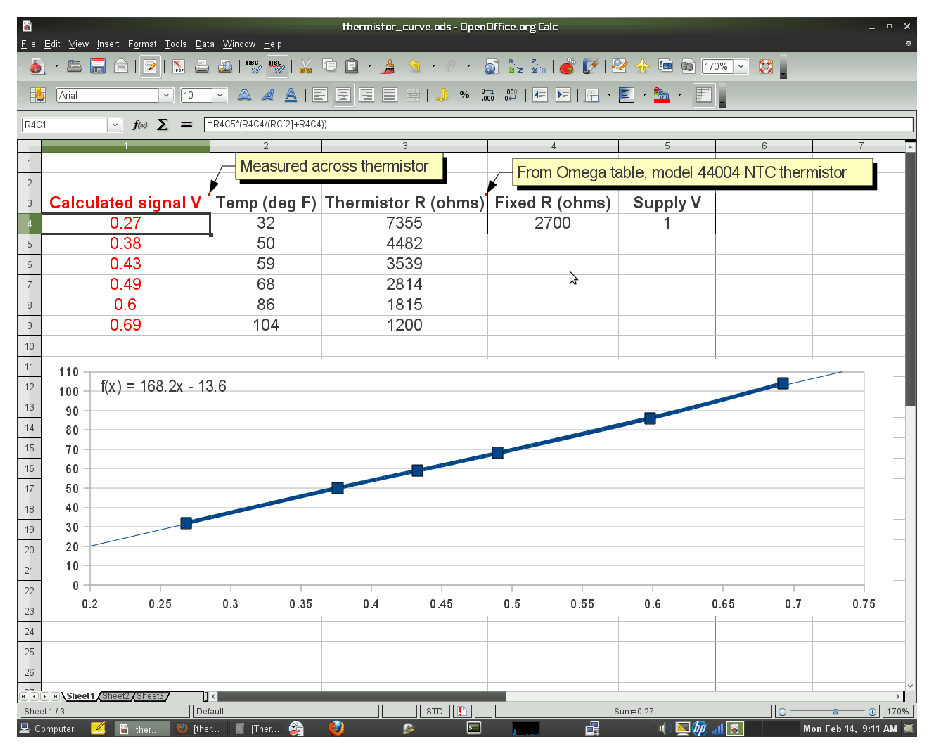
\includegraphics[width=15.5cm]{i00350x04.eps}$$

In this particular example, the sensor is a negative temperature coefficient (NTC) thermistor, model 44004, manufactured by Omega.  The formula entered into cells R4C1 through R9C1 calculates the voltage dropped across a fixed resistor (2700 $\Omega$) connected in series with the thermistor and powered by a 1 volt DC source, using the voltage divider equation ($V_R = V_{source} {R \over {R_{total}}}$).  The thermistor resistance values seen in column 3 were taken from an Omega-published table for the model 44004 thermistor.  A ``scatter'' plot graphs temperature as a function of voltage, and a ``trendline'' plotted by the spreadsheet program attempts to match the data points to a mathematical formula.  In this particular case, the fitted formula happens to be Temp = 168.2 * (Voltage) $-$ 13.6.  It is this formula you must enter into the DAQ software, so it knows how to translate the measured voltage signal into a temperature value.

\filbreak

If the sensor you choose does not have a data table describing its characteristics, you may generate your own by subjecting it to known stimuli and measuring its resistance at those known values.  Then, you may use a spreadsheet to plot the voltage response and derive an equation to fit the data.

Another huge advantage of using a computer spreadsheet to model the signal voltage as a function of temperature is that it allows you to ``experiment'' with different values of fixed resistance, to see the effect it has on linearity.  By entering a new fixed-resistor value into the spreadsheet, you may immediately see the effect that value change has on the curvature of the scatter plot, as well as the effect it has on the signal voltage strength.

\vskip 10pt

{\bf Common mistakes:}

\begin{itemize}
\item{} Choosing a poor-accuracy calibration standard (e.g. trying to calibrate your \$1500 precision Rosemount pressure transmitter to $\pm$ 0.1 PSI using a \$30 pressure gauge that only reads to the nearest 5 PSI!).
\item{} Improperly configuring the spreadsheet scatter plot to generate a fitted equation (e.g. having variables on wrong axes)
\end{itemize}

\vskip 10pt

{\bf Characterizing your sensor and scaling the DAQ software should take no more than one full lab session (3 hours) if the team is working efficiently!}






\vfil \eject

\noindent
{\bf Lab Exercise -- Ethernet data transfer}

\vskip 5pt

An essential part of this lab exercise is to have the acquired data transported over an Ethernet network.  Unless the DAQ software is quite sophisticated, this feature is not likely to be directly supported.  A suitable alternative is to have one computer acquiring data from the DAQ module, and use another computer to remotely view the display of the first computer.  This remote viewing may be done using ``Remote Desktop'' in Microsoft Windows operating systems, or by installing free remote-administration software such as {\tt RealVNC}.

Not only will remote access allow you to view the live DAQ data from another computer over the Ethernet network, but it also allows you do {\it operate} the DAQ computer remotely.  Knowing how to use remote-viewing software, therefore, is a very useful skill.

\vskip 10pt

Another Ethernet-related objective in this lab exercise is using the {\tt ping} utility to test for network connections.  When two personal computers have been successfully connected to a common Ethernet network, you should be able to ``ping'' one computer from the other by invoking the {\tt ping} utility with the IP address of the destination computer as an argument to the {\tt ping} command.  You may run the {\tt ping} command from a command-line window on a Microsoft Windows operating system.  More detailed instructions on the use of {\tt ping} may be found in your {\it Lessons In Industrial Instrumentation} textbook.

A successful ``ping'' from one computer to another is a {\it necessary} condition for remote viewing of that computer's display, but it is not a {\it sufficient} condition.  That is to say, although a computer that refuses to ``ping'' is definitely not ready to be logged into remotely, a computer that does ``ping'' without trouble may not necessarily be ready for remote login.  Getting a successful ``ping'' from a computer is merely the first step in establishing full communication with it.

\vskip 10pt

If a ``ping'' attempt proves unsuccessful, it means something is inhibiting communication between that device and the computer you're using to issue the ping.  A good test to do in this circumstance is try ``pinging'' other devices on that same network.  Any successful ping attempts will definitively prove OSI layers 1, 2, and 3 are all functional between those two points, since ``ping'' requires those three layers to function.  Once you know which portion(s) of the network are functional, you may narrow the field of fault possibilities.

\vskip 10pt

Network functions above OSI layer 3 (e.g. ``firewall'' software running on personal computers) are capable of inhibiting communication between devices on the lab's Ethernet network, including ``ping'' messages.  If you decide to connect your own personal computer (laptop) to the lab's Ethernet network, you may find it easier to temporarily disable all security features on your personal computer to enable free and open communication between your computer and all other devices on the network.  Just be sure to re-enable the security features when you are done, so your computer will not be unprotected the next time you connect to the Internet!







\vfil \eject

\noindent
{\bf Lab Exercise -- troubleshooting}

\vskip 5pt

The most challenging aspect of this lab exercise is {\it troubleshooting}, where you demonstrate your ability to logically isolate a problem in the system.  All troubleshooting is done on an individual basis (no team credit!), and must be done {\it on a system you did not help build}, so that you must rely on loop diagrams to find your way around the system instead of from your own memory of building it.

Each student is given a limited amount of time to identify both the general location and nature of the fault, logically justifying all diagnostic steps taken.  All troubleshooting activities will take place under direct instructor supervision to ensure students are working independently and efficiently. 

Failure to correctly identify both the general location and nature of the fault within the allotted time, and/or failing to demonstrate rational diagnostic procedure to the supervising instructor will disqualify the effort, in which case the student must re-try with a different fault.  Multiple re-tries are permitted with no reduction in grade.

A standard multimeter is the only test equipment allowed during the time limit.  No diagnostic circuit breaks are allowed except by instructor permission, and then only after correctly explaining what trouble this could cause in a real system.  

The instructor will review each troubleshooting effort after completion, highlighting good and bad points for the purpose of learning.  Troubleshooting is a skill born of practice and failure, so do not be disappointed in yourself if you must make multiple attempts to pass!  One of the important life-lessons embedded in this activity is how to deal with failure, because it {\it will} eventually happen to you on the job!  There is no dishonor in failing to properly diagnose a fault after doing your level best.  The only dishonor is in taking shortcuts or in giving up.

\vskip 10pt

{\bf Common mistakes:}

\begin{itemize}
\item{} Neglecting to take measurements with your multimeter.
\item{} Neglecting to check other measurements in the system (e.g. pressure gauge readings).
\item{} Incorrectly interpreting the diagram (e.g. thinking you're at the wrong place in the system when taking measurements).
\item{} Incorrect multimeter usage (e.g. AC rather than DC, wrong range, wrong test lead placement).  This is especially true when a student comes to lab unprepared and must borrow someone else's meter that is different from theirs!
\end{itemize}

\vskip 10pt

{\bf Remember that the purpose of the troubleshooting exercise is to foster and assess your ability to intelligently diagnose a complex system.  Finding the fault by luck, or by trial-and-error inspection, is not a successful demonstration of skill.  The only thing that counts as competence is your demonstrated ability to logically analyze and isolate the problem, correctly explaining all your steps!}

\vskip 10pt

{\bf Troubleshooting takes a lot of lab time, usually at least two 3-hour lab sessions for everyone in a full class to successfully pass.  Be sure your team budgets for this amount of time as you plan your work, and also be sure to take advantage of your freedom to observe others as they troubleshoot, to better learn this art.}




\vfil \eject

\noindent
{\bf Lab questions}

\vskip 5pt

\begin{itemize}
\item{} {\bf Instrument connections}
\item{} Determine correct wire connections between a DAQ module and an electrical sensor, based on diagrams of instruments with terminals labeled
\item{} Correctly determine all electrical sources and loads, as well as all voltage polarities and current directions in a DAQ/sensor circuit, based on diagrams of instruments with terminals labeled
\end{itemize}

\filbreak

\begin{itemize}
\item{} {\bf Commissioning and Documentation}
\item{} Explain the operating principle of the sensor used in your system
\item{} Explain the difference between a {\it single-ended} input channel and a {\it differential} input channel on an analog DAQ module
\item{} Describe the use of some of the advanced functions of your multimeter {\it besides} record (``Min/Max'') mode
\item{} Explain why power and signal wiring should not be run together in conduit or in a panel
\item{} Explain why it is necessary to use a {\it bushing} to protect electrical wires that enter and exit an electrical enclosure through a hole in the side of that enclosure
\end{itemize}

\filbreak

\begin{itemize}
\item{} {\bf Mental math} (no calculator allowed!)
\item{} Determine allowable calibration error of instrument (e.g. +/- 0.5\% for an instrument ranged 200 to 500 degrees)
\item{} Convert 1-5 V signal into a percentage of span (e.g. 3.5 V = \underbar{\hskip 20pt}\%)
\item{} Convert percentage of span into a 1-5 V signal value (e.g. 70\% = \underbar{\hskip 20pt} V)
\item{} Calculate resolution of ADC given number of bits and input signal range
\end{itemize}

\filbreak

\begin{itemize}
\item{} {\bf Diagnostics}
\item{} Explain how to distinguish an ``open'' cable fault from a ``shorted'' cable fault using only a voltmeter (no current or resistance measurement, but assuming you are able to break the circuit to perform the test)
\item{} Determine whether or not a given diagnostic test will provide useful information, given a set of symptoms exhibited by a failed system
\item{} Identify at least two plausible faults given the results of a diagnostic test and a set of symptoms exhibited by a failed system
\item{} Propose a diagnostic test for troubleshooting a failed system and then explain the meanings of two different test results
\end{itemize}



\vfil \eject

\noindent
{\bf Lab Exercise -- decommissioning and clean-up}

\vskip 5pt

The final step of this lab exercise is to decommission your team's entire system and re-stock certain components back to their proper storage locations, the purpose of which being to prepare the lab for the next lab exercise.  Remove your system documentation (e.g. loop diagram) from the common holding area, either discarding it or keeping it for your own records.  Also, remove instrument tag labels (e.g. FT-101) from instruments and from cables.  Perform general clean-up of your lab space, disposing of all trash, placing all tools back in their proper storage locations, sweeping up bits of wire off the floor and out of junction boxes, etc.

\vskip 10pt

\indent
{\bf Leave the following components in place, mounted on the racks:}

\begin{itemize}
\item{} Large control valves and positioners
\item{} I/P transducers
\item{} Large electric motors
\item{} Large variable-frequency drive (VFD) units
\item{} Cables inside conduit interconnecting junction boxes together
\item{} Pipe and tube fittings (do not unscrew pipe threads)
\item{} Supply air pressure regulators
\end{itemize}

\vskip 10pt

\indent
{\bf Return the following components to their proper storage locations:}

\begin{itemize}
\item{} Sensing elements (e.g. thermocouples, pH probes, etc.)
\item{} Process transmitters
\item{} ``Jumper'' cables used to connect terminal blocks within a single junction box
\item{} Plastic tubing and tube fittings (disconnect compression-style tube fittings)
\item{} Power cables and extension cords
\item{} Adjustment (loading station) air pressure regulators
\end{itemize}

\vskip 10pt

Finally, you shall return any control system components to their original (factory default) configurations.  This includes controller PID settings, function block programs, input signal ranges, etc.


\underbar{file i00350}
\vskip 10pt \filbreak 





\svar{} 

There exist some inexpensive data acquisition modules on the market for personal computers, including some with USB interfaces (and most with RS-232 serial interfaces).  If all you have is a serial-interface module and a USB-only computer (as most laptop computers are!), you may use a USB-to-serial adapter to connect the serial DAQ device to the personal computer.  Within Microsoft Windows, you may force the operating system to recognize the USB adapter as an old-style COM 1 or COM 2 RS-232 serial device, at which time the DAQ software should ``talk'' through the adapter to the DAQ module seamlessly.

\vskip 10pt \filbreak 





\notes{} 

\noindent
{\bf Diagrams / inspections:}

I strongly recommend checking off students' diagrams while you inspect their system (checking for secure wiring, proper tubing, good conduit installation, etc.) with them.  Have all team members take you on a ``tour'' of their completed system, with each team member explaining a different portion of the system you select while using their own diagram as a guide.  While a student is explaining their section of the system, you can check the other students' diagrams for accuracy.  This not only saves time by consolidating the tasks of system inspection and diagram verification, but it also ensures students can actually relate their diagrams to the system they have built and articulate that understanding to you.

\vskip 10pt

\goodbreak

\noindent
{\bf Troubleshooting fault ideas:}

\begin{itemize}
\goodbreak
\item{} Strip wire at terminal, then insert insulated wire end under terminal and tighten (open wire fault)
\item{} Cut signal cable somewhere in mid-conduit (open wire fault)
\item{} Unplug Ethernet cable
\item{} Change IP address or network mask of one computer
\item{} Wire instrument cable conductors backward (construction fault)
\item{} Configure transmitter for excessive damping (slow response fault)
\item{} Configure indicator/controller for excessive damping (slow response fault)
\item{} Miscalibrate transmitter and/or indicator/controller (inaccuracy fault)
\item{} Plug tube connections using portion of foam earplug stuffed into tube fitting (slow response fault)
\item{} Mis-configure linear characterization of transmitter and/or DAQ (nonlinearity fault)
\item{} Mis-configure function block inside DAQ (e.g. change limit values to simulate signal stuck either low or high; disconnect signal line between two blocks)
\item{} Connect 2.2 k resistor in parallel with 4-20 mA transmitter to simulate partial short in wiring (inaccuracy fault)
\item{} Exchange 250 ohm resistor for a different resistor that looks the same but has the wrong value (inaccuracy fault) 
\item{} Give students wrong diagram (documentation fault)
\end{itemize}















\vfil \eject

\noindent
{\bf Lab questions}

\vskip 20pt

\item{$(1)$} Connect the transmitter to register pressure on channel 3 on the DAQ:

$$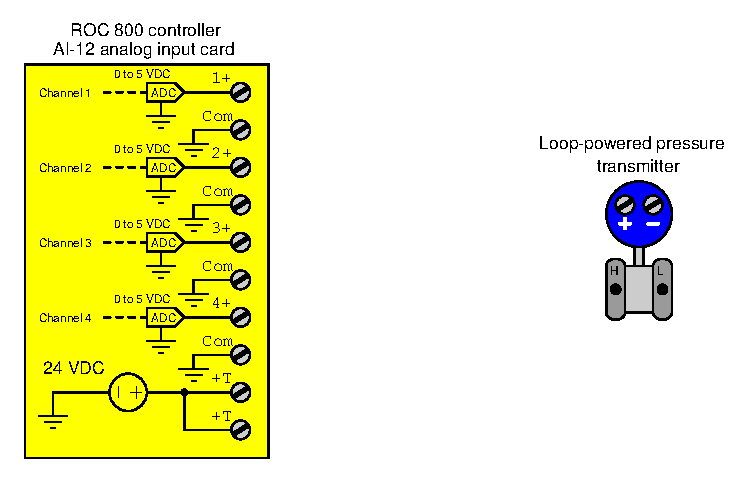
\includegraphics[width=15.5cm]{i00350x07.eps}$$

\vskip 20pt

\item{$(2)$} Explain the difference between {\it single-ended} and {\it differential} inputs on an analog DAQ module.

\vskip 20pt

\item{$(3)$} Determine the allowable calibration error of a pressure transmitter with a range of 0 to 300 PSI and a calibration tolerance of $\pm$ 0.5\%.  Express your answer in units of PSI.

\vskip 20pt

\item{$(4)$} PC number 3 (IP address 192.168.0.2) cannot connect to the internet.  Identify one diagnosic test you could perform on this system, then describe {\it two (different) possible results} of that test and explain what each result would mean in terms of locating the fault:

$$\includegraphics[width=15.5cm]{i00350x09.eps}$$

















\vfil \eject

\noindent
{\bf Lab questions}

\vskip 20pt

\item{$(1)$} Connect the transmitter to register pressure on channel 2 on the DAQ:

$$\includegraphics[width=15.5cm]{i00350x08.eps}$$

\vskip 20pt

\item{$(2)$} Identify at least one of the advanced functions offered by your multimeter {\it besides} record (``Min/Max'') mode.

\vskip 20pt

\item{$(3)$} Convert a 2.5 volt signal (in a 1-5 volt range) into a value expressed in {\it percent}.

\vskip 20pt

\item{$(4)$} PC number 5 (IP address 192.168.0.29) cannot connect to PC number 1 (IP address 192.168.0.35).  Identify one diagnosic test you could perform on this system, then describe {\it two (different) possible results} of that test and explain what each result would mean in terms of locating the fault:

$$\includegraphics[width=15.5cm]{i00350x09.eps}$$


%INDEX% Lab exercise, data acquisition and Ethernet networking

\vfil \eject 



\oppgave{} 
% Copyright 2015, Tony R. Kuphaldt, released under the Creative Commons Attribution License (v 1.0)
% This means you may do almost anything with this work of mine, so long as you give me proper credit

\noindent
{\bf RTU component layout}

\vskip 10pt

An ``RTU'' is a {\it Remote Terminal Unit} in a SCADA system serving as the interface between field instruments and a central control/display unit called the ``MTU'' ({\it Master Terminal Unit}).  In our caSCADA system, the MTU is just a laptop computer viewing data generated by the Raspberry Pi computer in each RTU.  Each RTU uses a LabJack data acquisition unit to sense analog signals sent by field transmitters and a single-board computer called a Raspberry Pi to condition and present that data in the form of digital data files readable by the MTU.  Communication takes place via a wireless access point (WAP) router:

$$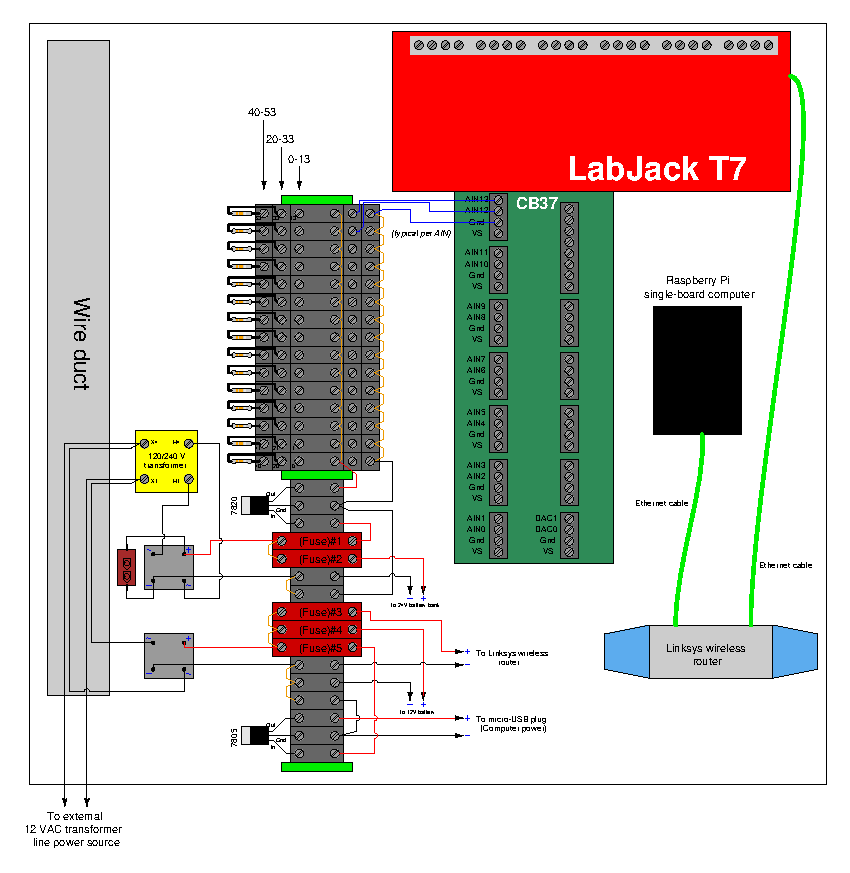
\includegraphics[width=15.5cm]{i02566x01.eps}$$

Each RTU enclosure is weatherproof, and equipped with a set of batteries to maintain DC power to all the system components in the event of an external AC power failure.

The upper level of terminals on the triple-level blocks should all be jumpered together because this is the 20 VDC ``bus'' used to power all field instruments.  The lower level of terminals should also be jumpered together because they comprise the negative side (``Common'' or ``GND'') of that same 20 VDC loop power supply.





\vfil \eject

\noindent
{\bf Sample loop diagrams}

$$\includegraphics[width=15.5cm]{i02566x02.eps}$$

A set of triple-height terminal blocks marshall field instrument signals to the DAQ input terminals.  Both current-based and voltage-based instrument signals may be accepted by the DAQ.  In the case of 4-20 mA loop instruments, a precision 250 $\Omega$ resistor is connected in such a way to provide a 1-5 VDC signal for the DAQ to sense.  If the field instrument outputs a voltage signal instead (which is actually quite common for RTU loops in remote installations relying on solar power) then the resistor is omitted and the LabJack AIN directly reads that instrument's output voltage.

\vskip 10pt

All $n$ terminals are jumpered together and powered by the same 20 VDC source, fed through fuse \#1.  All $4n$ terminals are also jumpered together and connect to the negative rail of the 20 VDC power source.  Only the $2n$ terminals are independent from each other, since they carry the individual analog input signals unique to each AIN channel on the LabJack.



\vfil \eject

\noindent
{\bf Electrical power diagram}

$$\includegraphics[width=15.5cm]{i02566x03.eps}$$

Power is sent to each RTU box at 12 volts AC, from a transformer located near a 120 VAC power source.  This keeps the field power cable at a safe, low voltage (similar to outside sprinkler control systems and walkway lighting). 

\vskip 10pt

Internal to each RTU is a dual-voltage DC system: 12 volts (regulated down to 5 VDC) for running the Linux-based computer, LabJack DAQ, and Linksys WRT54GL wireless router; and 20 volts for powering the field instruments.  Lead-acid batteries provide back-up power for the RTU to continue running in the event of a power outage.  The resistor-diode network limits battery charging current to a bare minimum, while providing full current capacity in the discharge direction (in the event of an AC line power outage).

24 volts is a more customary DC supply voltage for loop-powered field instruments, but the LabJack model T7 DAQ has an absolute maximum input voltage of 20 VDC.  Thus, the loop supply voltage is limited to this value to avoid the potential for damage to the LabJack in the event of a shorted instrument cable which would apply full power supply voltage to the DAQ input.





\vfil \eject

\noindent
{\bf RTU power system testing procedure}

\vskip 10pt

You must follow this procedure when first commissioning a new RTU.  When working with an existing RTU, you may follow the same procedure to test the continuing health of the DC power system.

\vskip 10pt

\begin{itemize}
\item{(1)} Test the external 12 VAC transformer by itself: when plugged into a 120 volt AC source, does it output at least 12 volts AC?
\vskip 10pt
\item{(2)} Open up all fuses (\#1 through \#5) to ensure no device will become powered until you intend so.
\vskip 10pt
\item{(3)} Connect this external 12 VAC transformer's output to the RTU as shown in the diagrams and apply power.  Check the output of both bridge rectifiers for proper DC voltage magnitude and polarity.  Due to the filter capacitors the DC voltage magnitudes will register greater than the AC voltage magnitudes feeding each of the bridge rectifiers.
\vskip 10pt
\item{(4)} Ensure the batteries are wired to the proper terminal blocks and fuse holders, and measure DC voltage magnitudes and polarities at the battery-side of each open fuse.  This ensures the batteries are properly connected.
\vskip 10pt
\item{(5)} Close fuses \#2 and \#4.  This connects the two battery banks to their respective charging sources.  Re-measure the voltage magnitudes at the battery-side of each closed fuse.  You should read slightly higher voltage now than in the previous step, because the batteries are charging.
\vskip 10pt
\item{(6)} Ensure all power plugs are removed from the caSCADA electronic devices: the LabJack DAQ unit, the Raspberry Pi computer, and the Linksys wireless router.  Prepare to measure DC voltage at the ends of those power plugs.
\vskip 10pt
\item{(7)} Close fuse \#3 and measure DC voltage magnitude and polarity at the Linksys router's power plug.  Check the router's documentation for the proper DC polarity of the plug's shell and tip to see that the polarity is correct.  If all is well, plug the power cable into the router and check to see that it powers up.  Re-measure voltage magnitude at fuse \#3 to see that the router is receiving adequate voltage while powered (i.e. under load).
\vskip 10pt
\item{(8)} Close fuse \#5 and measure DC voltage magnitude and polarity at the Raspberry Pi's micro-USB power plug.  Check online for the ``pinout'' specification of a micro-USB power plug to see that the polarity is correct.  If the pins on the micro-USB plug are too small to safely probe using your multimeter, you may check DC voltage at the stripped end of that cable where it lands at the terminal block, and verify correct voltage and polarity according to the colors of that cable's wires.  If all is well, plug the power cable into the Raspberry Pi and check to see that it powers up.
\vskip 10pt
\item{(9)} Plug the B-style USB cable into the LabJack.  It receives power through the Raspberry Pi and should power up immediately.  Re-measure voltage magnitude at fuse \#5 to see that both the Raspberry Pi and LabJack units are receiving adequate voltage while powered (i.e. under load).
\vskip 10pt
\item{(10)} Close fuse \#1 to apply 20 VDC power to the field instrument terminal blocks.  Measure DC voltage magnitude and polarity between terminals 13 and 53 to ensure 20 VDC is supplied all the way to the end of the terminal block section.
\vskip 10pt
\item{(11)} At this point in time you may initialize the caSCADA system MTU (a laptop PC) and test the system for proper data.  A procedure for this is given on the following page.
\vskip 10pt
\item{(12)} Unplug the external 12 VAC transformer from its line power source, and re-measure all DC supply voltages to ensure all devices are receiving adequate voltage under battery power alone.
\vskip 10pt
\item{(13)} Repeat these DC voltage measurements at one-hour intervals to check the health of the batteries.
\end{itemize}





\vfil \eject

\noindent
{\bf RTU data system testing}

\vskip 10pt

You must follow this procedure when first commissioning new devices for an RTU.

\vskip 10pt

\begin{itemize}
\item{(1)} Ensure that the proper IP addresses are all written on labels affixed to each of the networked devices in the RTU: the LabJack DAQ unit, the Linksys wireless router, and the Raspberry Pi single-board computer.
\vskip 10pt
\item{(2)} Set the IP address and subnet mask of your personal computer to appropriate values for the Ethernet device you wish to connect to.  For each octet of the subnet mask with the value ``255'' the octet of your PC's IP address must match the IP addresses of all devices in the RTU.  For each octet of the subnet mask with the value of ``0'' the octet of your PC's IP address must be different from any device in the RTU.  This will prepare your PC for direct Ethernet cable connection to the device you intend to configure.  
\vskip 10pt
\item{(3)} Plug your computer into the Linksys router using an Ethernet cable, and set the router's IP address and subnet mask and name using a web browser.  Follow the instructions given in the manual for the router.  The router's name should make sense to any user of the system.  In an area with multiple RTUs, the name should be specific enough to clearly identify which RTU it is.
\vskip 10pt
\item{(4)} Plug your computer into the LabJack DAQ using an Ethernet cable, and set the DAQ's IP address and subnet mask using the software provided by LabJack for this task.  Follow the instructions given in the LabJack manual.
\vskip 10pt
\item{(5)} Plug an HDMI monitor and USB keyboard into the Raspberry Pi, and log in directly to set its IP address and subnet mask.  To check its current settings, use the {\tt ifconfig} command (similar to the {\tt ipconfig} command in Microsoft Windows).  If the settings are not correct, you may change them by editing the file {\tt /etc/network/interfaces}.  This requires ``root'' privileges.  Lines of text in this {\tt interfaces} file follow this pattern:
\begin{itemize}

\item{} Prior to the {\tt eth0} line must be a line that reads {\tt auto eth0}
\item{} The ``address'' line contains the IP address (e.g. {\tt address 169.254.8.3})
\item{} The ``netmask'' line contains the subnet mask (e.g. {\tt netmask 255.255.255.0})
\vskip 10pt
\item{(6)} Unplug the Ethernet cable from your personal computer and wirelessly connect to the Linksys router.  The router will automatically assign an appropriate IP address to your computer's wireless card, as routers are designed to do.
\vskip 10pt
\item{(7)} Use the {\tt ping} command in your computer to test network connectivity with each device in the RTU.  This command is simply the word ``ping'' followed by the IP address of the device you wish to ping.  For example, {\tt ping 169.254.8.1} will test to see whether your computer has connectivity with the device bearing the IP address 169.254.8.1.
\vskip 10pt
\item{(8)} Once all devices have been proven to ping successfully, you may use an SSH client program in your personal computer (e.g. {\tt Bitvise}) to log into the Raspberry Pi.  The login account is simply {\tt btc} with the password {\tt btc}.
\vskip 10pt
\item{(9)} Once you are logged in to the Linux operating system in the Raspberry Pi, you may try compiling the caSCADA code and then running it (either the {\tt simulate} process or the {\tt poll} process) to see that the data files are being appropriately populated by the caSCADA software.
\end{itemize}
\end{itemize}






\vfil \eject

\noindent
{\bf Preparing the Raspberry Pi for use in the caSCADA system}

\vskip 10pt

If you are initially configuring a Raspberry Pi to be used in the caSCADA system, there are several things you must do.  This is outside the realm of student work, and will be completed by the instructor prior to your use of the Raspberry Pi.  Here is a list:

\begin{itemize}
\item{} Log in as the default user (name = {\tt pi} and password = {\tt raspberry})
\vskip 5pt
\item{} Use the {\tt sudo} and {\tt passwd} commands to reset the root account's password to your liking (e.g. {\tt sudo passwd root}).  There are several tasks for which root privileges are necessary, so it's convenient to be able to log into the root account and do that work there, rather than have to preface all those commands typed under the {\tt pi} login user with the ``{\tt sudo}'' qualifier.
\vskip 5pt
\item{} Use the {\tt raspi-config} utility to set the system's hostname, configure the keyboard for US mapping (as British ``UK'' mapping is the default!), and also enable the {\tt ssh} server which will be essential for remote login and system administration.
\vskip 5pt
\item{} Add a new user account called {\tt btc}.
\vskip 5pt
\item{} Feel free to edit the hidden file named {\tt .profile} in the {\tt /home/btc} directory with any special instructions to be executed at login.  For example, you may add lines containing the {\tt echo} shell command to print messages to the screen for the user once they log in (e.g. {\tt echo "Welcome to the fish hatchery RTU"}). 
\vskip 5pt
\item{} Set the current time and date using the {\tt date} command.  The format is MMDDhhmmCCYY.  For example, 3:21 PM on November 5, 2016 would be set by issuing the command {\tt date 110515212016}.
\vskip 5pt
\item{} Navigate to the {\tt /etc/network} directory and edit the file named {\tt interfaces} to set all the required IP address and netmask information to give the Raspberry Pi a static IP address for use in the caSCADA system.
\vskip 5pt
\item{} Install the {\tt cascada.tar} archive file in the {\tt /home/btc} directory, and then use the command {\tt tar xvf cascada.tar} to unpack that archive file.
\vskip 5pt
\item{} Install the latest {\tt libmodbus} library archive file in the {\tt root} directory, then uncompress it ({\tt gunzip libmodbus*.gz}) and unpack the archive ({\tt tar xvf libmodbus*tar}) and then descend into the new {\tt libmodbus} directory to build it.  Build and install the new software using the commands {\tt ./configure ; make ; make install ; ldconfig}.
\vskip 5pt
\item{} Install the latest {\tt ncurses} library archive file in the {\tt root} directory, then uncompress it ({\tt gunzip ncurses*.gz}) and unpack the archive ({\tt tar xvf ncurses*tar}) and then descend into the new {\tt ncurses} directory to build it.  Build and install the new software using the commands {\tt ./configure ; make ; make install ; ldconfig}.
\vskip 5pt
\item{} Install the latest {\tt lynx} text-based web browser software archive file in the {\tt root} directory, then uncompress it ({\tt gunzip lynx*.gz}) and unpack the archive ({\tt tar xvf lynx*tar}) and then descend into the new {\tt lynx} directory to build it.  Build and install the new software using the commands {\tt ./configure ; make ; make install ; ldconfig}.
\vskip 5pt
\item{} Navigate to the {\tt /home/btc} directory and edit the file {\tt cascada\_poll.c} with the correct IP address to establish a Modbus/TCP connection with the LabJack DAQ unit in your RTU.  The function establishing the address will be easy to find in this file, as it calls out the IP address in standard four-octet format.  Just edit the IP address that's shown, and the caSCADA software will be able to communicate with that LabJack DAQ.
\vskip 5pt
\item{} Try running {\tt make poll} and {\tt make simulate} in the {\tt /home/btc} directory to see that the caSCADA software successfully compiles.
\end{itemize}




\underbar{file i02566}
\vskip 10pt \filbreak 





\svar{} 


\vskip 10pt \filbreak 





\notes{} 


%INDEX% Lab exercise, diagrams for caSCADA system RTUs

\vfil \eject 



\oppgave{} 
% Copyright 2015, Tony R. Kuphaldt, released under the Creative Commons Attribution License (v 1.0)
% This means you may do almost anything with this work of mine, so long as you give me proper credit

\noindent
{\bf Lab Exercise -- introduction}

\vskip 5pt

Your task is to build, document, and troubleshoot a pressure measurement system consisting of an electronic $\Delta$P or gauge pressure transmitter connected to an electronic indicator, recorder, or indicating controller.  Instrument air pressure, either regulated or unregulated, is the suggested process variable to measure.  Other process variables are open for consideration, though.  Alternatives to the standard pressure-measurement lab are authorized by instructor permission only.

The following table of objectives show what you and your team must complete within the scheduled time for this lab exercise.  Note how some of these objectives are individual, while others are for the team as a whole:

\underbar{Objective completion table:}

% No blank lines allowed between lines of an \halign structure!
% I use comments (%) instead, so that TeX doesn't choke.

$$\vbox{\offinterlineskip
\halign{\strut
\vrule \quad\hfil # \ \hfil & 
\vrule \quad\hfil # \ \hfil & 
\vrule \quad\hfil # \ \hfil & 
\vrule \quad\hfil # \ \hfil & 
\vrule \quad\hfil # \ \hfil & 
\vrule \quad\hfil # \ \hfil & 
\vrule \quad\hfil # \ \hfil \vrule \cr
\noalign{\hrule}
%
% First row
{\bf Performance objective} & {\bf Grading} & {\bf 1} & {\bf 2} & {\bf 3} & {\bf 4} & {\bf Team} \cr
%
\noalign{\hrule}
%
% Another row
Team meeting and prototype sketch (do {\it first!}) & mastery & -- & -- & -- & -- & \cr
%
\noalign{\hrule}
%
% Another row
Circuit design challenge & mastery & & & & & -- -- -- -- \cr
%
\noalign{\hrule}
%
% Another row
Final loop diagram and system inspection & mastery & & & & & -- -- -- -- \cr
%
\noalign{\hrule}
%
% Another row
Digital trim (sensor and output) & mastery & -- & -- & -- & -- &  \cr
%
\noalign{\hrule}
%
% Another row
Loop ranging ($\pm$ 1\% of span accuracy) & mastery & & & & & -- -- -- -- \cr
%
\noalign{\hrule}
%
% Another row
Deadweight tester research and usage & mastery & & & & & -- -- -- -- \cr
%
\noalign{\hrule}
%
% Another row
Transmitter valve manifold usage & mastery & & & & & -- -- -- -- \cr
%
\noalign{\hrule}
%
% Another row
Troubleshooting & mastery & & & & & -- -- -- -- \cr
%
\noalign{\hrule}
%
% Another row
Lab question: Instrument connections & proportional &  &  &  &  & -- -- -- -- \cr
%
\noalign{\hrule}
%
% Another row
Lab question: Commissioning & proportional &  &  &  &  & -- -- -- -- \cr
%
\noalign{\hrule}
%
% Another row
Lab question: Mental math & proportional &  &  &  &  & -- -- -- -- \cr
%
\noalign{\hrule}
%
% Another row
Lab question: Diagnostics & proportional &  &  &  &  & -- -- -- -- \cr
%
\noalign{\hrule}
%
% Another row
Decommission and lab clean-up & mastery & -- & -- & -- & -- &  \cr
%
\noalign{\hrule}
} % End of \halign 
}$$ % End of \vbox

The only ``proportional'' scoring in this activity are the lab questions, which are answered by each student individually.  A listing of potential lab questions are shown at the end of this worksheet question.  The lab questions are intended to guide your labwork as much as they are intended to measure your comprehension, and as such the instructor may ask these questions of your team day by day, rather than all at once (on a single day).

\vskip 10pt

{\bf It is essential that your team plans ahead what to accomplish each day.  A short (10 minute) team meeting at the beginning of each lab session is a good way to do this, reviewing what's already been done, what's left to do, and what assessments you should be ready for.  There is a lot of work involved with building, documenting, and troubleshooting these working instrument systems!}

As you and your team work on this system, you will invariably encounter problems.  You should always attempt to solve these problems as a team before requesting instructor assistance.  If you still require instructor assistance, write your team's color on the lab whiteboard with a brief description of what you need help on.  The instructor will meet with each team in order they appear on the whiteboard to address these problems.

$$\includegraphics[width=15.5cm]{i00112x01.eps}$$





\vfil \eject

\noindent
{\bf Lab Exercise -- team meeting, prototype sketch, and instrument selection}

\vskip 5pt

An important first step in completing this lab exercise is to {\bf meet with your instructor} as a team to discuss safety concerns, team performance, and specific roles for team members.  If you would like to emphasize exposure to certain equipment (e.g. use a particular type of control system, certain power tools), techniques (e.g. fabrication), or tasks to improve your skill set, this is the time to make requests of your team so that your learning during this project will be maximized.

\vskip 10pt

An absolutely essential step in completing this lab exercise is to work together as a team to {\bf sketch a prototype diagram} showing what you intend to build.  This usually takes the form of a simple electrical schematic and/or loop diagram showing all electrical connections between components, as well as any tubing or piping for fluids.  This prototype sketch need not be exhaustive in detail, but it does need to show enough detail for the instructor to determine if all components will be correctly connected for their safe function.

For example, if you intend to connect field devices to a PLC (Programmable Logic Controller), your prototype sketch must show how those devices will connect to typical input/output terminals on the PLC, where electrical power will be supplied, etc.  Prototype sketches need not show all intermediary connections between components, such as terminal blocks in junction boxes between the field device and the controller.

You should practice good problem-solving techniques when creating your prototype sketch, such as consulting equipment manuals for information on component functions and marking directions of electric current, voltage polarities, and identifying electrical sources/loads.  Use this task as an opportunity to strengthen your analytical skills!  Remember that you will be challenged in this program to do all of this on your own (during ``capstone'' assessments), so do not make the mistake of relying on your teammates to figure this out for you -- instead, treat this as a problem {\it you} must solve and compare your results with those of your teammates.

Your team's prototype sketch is so important that the instructor will demand you provide this plan before any construction on your team's working system begins.  {\it Any team found constructing their system without a verified plan will be ordered to cease construction and not resume until a prototype plan has been drafted and approved!}  Similarly, you should not deviate from the prototype design without instructor approval, to ensure nothing will be done to harm equipment by way of incorrect connections.  Each member on the team should have ready access to this plan (ideally possessing their own copy of the plan) throughout the construction process.  Prototype design sketching is a skill and a habit you should cultivate in school and take with you in your new career.

\vskip 10pt

When selecting field instruments for this lab exercise, choose a {\it pressure transmitter} with electronic (4-20 mA) signal output as well as a valve ``manifold'' to isolate that transmitter from the process pressure.  Refer to the ``Valve manifolds'' subsection of {\it Lessons In Industrial Instrumentation} for more detail on what these manifolds look like and how they are used.  You should choose a transmitter with a pressure range somewhere between 10 PSI and 200 PSI.  Avoid low-range (``draft'') transmitters with ranges of just a few inches of water column, and also high-pressure transmitters ranged for hundreds or thousands of PSI.

Consult documentation from the manufacturer's website to identify how to properly wire, power, and calibrate the transmitter.  Your instructor will check to see you have located and are familiar with the equipment manual(s).

After locating a suitable instrument and its associated documentation, you should qualitatively test it prior to installing it in your system.  For a pressure transmitter, this entails applying an air pressure to the ``high'' pressure port and measuring the transmitter's milliamp output signal to see if it responds to the application of pressure.  If the transmitter fails to respond properly, tag it with a label explaining what it does (or what it fails to do).

\vskip 10pt

{\bf Planning a functioning system should take no more than an hour if the team is working efficiently, and will save you hours of frustration (and possible component destruction!).}








\vfil \eject

\noindent
{\bf Lab Exercise -- circuit design challenge}

\vskip 5pt

Connect an ``ice-cube'' relay to a low-voltage DC source as well as 120 volts AC so that a hand-operated switch will control the energization of a 120 VAC load.  All electrical connections must be made using a terminal strip (no twisted wires, crimp splices, wire nuts, spring clips, or ``alligator'' clips permitted), and the 120 VAC portion of the circuit must be fused for overcurrent protection.

This exercise tests your ability to properly interpret the ``pinout'' of an electromechanical relay, properly wire a switch to control a relay's coil, properly wire a load to the contacts of a relay, properly select NO/NC contacts on both the switch and the relay, and use a terminal strip to organize all electrical connections.

$$\includegraphics[width=15.5cm]{i00112x03.eps}$$

\vskip 10pt

The following components and materials will be available to you: assorted ``ice cube'' {\bf relays} with DC-rated coils and matching {\bf sockets} ; assorted pushbutton {\bf switches} ; {\bf terminal strips} ; lengths of {\bf hook-up wire} ; {\bf battery clips} (holders) ; 120 VAC {\bf power cord} with {\bf fuse assembly} ; 120 VAC {\bf lamp or other suitable load}.

\vskip 10pt

You will be expected to supply your own screwdrivers and multimeter for assembling and testing the circuit at your desk.  The instructor will supply the battery(ies) to power your circuit when you are ready to see if it works.  Until that time, your circuit will remain unpowered.

\vskip 20pt

\noindent
{\bf Load/switch status} (instructor chooses): \hskip 20pt \underbar{\hskip 20pt} On when pressed \hskip 10pt {\it or} \hskip 10pt \underbar{\hskip 20pt} Off when pressed

\vfil

Study reference: the ``Control Relays'' section of {\it Lessons In Industrial Instrumentation}.





\vfil \eject

\noindent
{\bf Lab Exercise -- building the system}

\vskip 5pt

The Instrumentation lab is set up to facilitate the construction of working instrument ``loops,'' with over a dozen junction boxes, pre-pulled signal cables, and ``racks'' set up with 2-inch vertical pipes for mounting instruments.  The only wires you should need to install to build a working system are those connecting the field instrument to the nearest junction box, and then small ``jumper'' cables connecting different pre-installed cables together within intermediate junction boxes.

After getting your prototype sketch approved by the instructor, you are cleared to begin building your system.  Transmitters attach to 2-inch pipes using special brackets and U-bolts.  These brackets and U-bolts are located along with the transmitters in the instrument storage area.  

Select a specific controller to act as a display indicator for the measured pressure.  Your instructor may choose the controller for your team, to ensure you learn more than one type of controller during the course of a quarter.

Finally, your pressure-measurement system needs to have a loop number, so all instruments may be properly labeled.  This loop number needs to be unique, so that another team does not label their instruments and cables the same as yours.  One way to make your loop number unique is to use the equivalent resistor color-code value for your team's color in the loop number.  For example, if you are the ``Red'' team, your loop number could be ``2''. 

\vskip 10pt

{\bf Common mistakes:}

\begin{itemize}
\item{} Neglecting to consult the manufacturer's documentation for field instruments (e.g. how to wire them, how to calibrate them).
\item{} Mounting the field instrument(s) in awkward positions, making it difficult to reach connection terminals or to remove covers when installed.
\item{} Improper pipe/tube fitting installation (e.g. trying to thread tube fittings into pipe fittings and vice-versa).
\item{} Failing to tug on each and every wire where it terminates to ensure a mechanically sound connection.
\item{} Students working on portions of the system in isolation, not sharing with their teammates what they did and how.  It is important that the whole team learns all aspects of their system!
\end{itemize}

\vskip 10pt

{\bf Building a functioning system should take no more than one full lab session (3 hours) if all components are readily available and the team is working efficiently!}





\vfil \eject

\noindent
{\bf Lab Exercise -- documenting the system}

\vskip 5pt

Each student must sketch their own {\it loop diagram} for their team's system, following proper ISA conventions.  Sample loop diagrams are shown in the next question in this worksheet.  These loop diagrams must be {\it comprehensive} and {\it detailed}, showing every wire connection, every cable, every terminal block, range points, etc.  The principle to keep in mind here is to make the loop diagram so complete and unambiguous that anyone can follow it to see what connects to what, even someone unfamiliar with industrial instrumentation.  In industry, loops are often constructed by contract personnel with limited understanding of how the system is supposed to function.  The loop diagrams they follow must be so complete that they will be able to connect everything properly without necessarily understanding how it is supposed to work.

Every instrument and every signal cable in your loop needs to be properly labeled with an ISA-standard tag number.  An easy way to do this is to wrap a short piece of masking tape around each cable (and placed on each instrument) then writing on that masking tape with a permanent marker.  Although no industry standard exists for labeling signal cables, a good recommendation is to label each two-wire cable with the tag number of the field instrument it goes to.  Thus, every length of two-wire cable in a pressure transmitter circuit should be labeled ``PT-$x$'' (where ``$x$'' is the loop number), every flow control valve should be labeled ``FV-$x$'', etc.  Remember that the entire loop is defined by the process variable it measures: if the PV is {\it temperature} then the transmitter with be a {\it T}T, the control valve will be a {\it T}V, the controller with be a {\it T}C, etc.

When your entire team is finished drafting your individual loop diagrams, call the instructor to do an inspection of the loop.  Here, the instructor will have students take turns going through the entire loop, with the other students checking their diagrams for errors and omissions along the way.  During this time the instructor will also inspect the quality of the installation, identifying problems such as frayed wires, improperly crimped terminals, poor cable routing, missing labels, lack of wire duct covers, etc.  The team must correct all identified errors in order to receive credit for their system.  

After successfully passing the inspection, each team member needs to place their loop diagram in the diagram holder located in the middle of the lab behind the main control panel.  When it comes time to troubleshoot another team's system, this is where you will go to find a loop diagram for that system!

\vskip 10pt

{\bf Common mistakes:}

\begin{itemize}
\item{} Forgetting to label all signal wires (see example loop diagrams).
\item{} Forgetting to label all field instruments with their own tag names (e.g. PT-83).
\item{} Forgetting to note all wire colors.
\item{} Forgetting to put your name on the loop diagram!
\item{} Basing your diagram off of a team-mate's diagram, rather than closely inspecting the system for yourself.
\item{} Not placing loop sheet instruments in the correct orientation (field instruments on the left, control room instruments on the right).
\end{itemize}

\vskip 10pt

{\bf Creating and inspecting accurate loop diagrams should take no more than one full lab session (3 hours) if the team is working efficiently!}





\vfil \eject

\noindent
{\bf Lab Exercise -- instrument calibration}

\vskip 5pt

Each team must calibrate the transmitter (``trim'' both the sensor and the output) to ensure it interprets pressure accurately and outputs an accurate current.  Then, each team member must configure the transmitter for a unique range (set the LRV and URV parameters) and scale the indicator (or indicating controller) to register in the proper engineering units (e.g. a pressure transmitter ranged for 30 to 70 PSI should actually register 30 to 70 PSI back at the control room display).  The accuracy of this ranging will be checked by the instructor by applying random air pressures to the transmitter while each student verifies the indicator display.

As in all cases where an instrument must be calibrated, you will need to check the instrument's response against one or more {\it standards}.  In this case, the ideal standard to use for setting the input pressure to the transmitter is a {\it precision test gauge} (either mechanical or electronic), and the ideal standard to use for measuring the transmitter's electronic output signal is a {\it multimeter} configured to measure DC milliamps:

$$\includegraphics[width=15.5cm]{i00112x02.eps}$$

The difference between ``calibrating'' a transmitter and ``ranging'' a transmitter is confusing to many students.  With legacy-style {\it analog} transmitters, calibrating and ranging are one and the same.  With modern {\it digital} instruments, calibration and ranging are separate tasks.  To calibrate a digital instrument means to subject it to a known (standard) stimulus and adjust the ``trim'' settings to ensure the instrument's microprocessor accurately recognizes that stimulus condition.  To ``range'' a digital instrument means to define the values of measurement for its 0\% and 100\% scale points.  For more information on this distinction, refer to the ``Instrument Calibration'' chapter of {\it Lessons In Industrial Instrumentation}.

\filbreak

Document the accuracy of your transmitter's sensor trim before and after adjustment in this table, at five different points throughout its sensing range using these two tables:

\vskip 10pt

{\bf As-Found calibration table}

% No blank lines allowed between lines of an \halign structure!
% I use comments (%) instead, so that TeX doesn't choke.

$$\vbox{\offinterlineskip
\halign{\strut
\vrule \quad\hfil # \ \hfil & 
\vrule \quad\hfil # \ \hfil & 
\vrule \quad\hfil # \ \hfil & 
\vrule \quad\hfil # \ \hfil \vrule \cr
\noalign{\hrule}
%
% First row
Applied pressure & Output signal (actual) & Output signal (ideal) & Error (\% of span) \cr
%
\noalign{\hrule}
%
% Another row
 &  &  & \cr
%
\noalign{\hrule}
%
% Another row
 &  &  & \cr
%
\noalign{\hrule}
%
% Another row
 &  &  & \cr
%
\noalign{\hrule}
%
% Another row
 &  &  & \cr
%
\noalign{\hrule}
%
% Another row
 &  &  & \cr
%
\noalign{\hrule}
} % End of \halign 
}$$ % End of \vbox

\vskip 10pt

{\bf As-Left calibration table}

% No blank lines allowed between lines of an \halign structure!
% I use comments (%) instead, so that TeX doesn't choke.

$$\vbox{\offinterlineskip
\halign{\strut
\vrule \quad\hfil # \ \hfil & 
\vrule \quad\hfil # \ \hfil & 
\vrule \quad\hfil # \ \hfil & 
\vrule \quad\hfil # \ \hfil \vrule \cr
\noalign{\hrule}
%
% First row
Applied pressure & Output signal (actual) & Output signal (ideal) & Error (\% of span) \cr
%
\noalign{\hrule}
%
% Another row
 &  &  & \cr
%
\noalign{\hrule}
%
% Another row
 &  &  & \cr
%
\noalign{\hrule}
%
% Another row
 &  &  & \cr
%
\noalign{\hrule}
%
% Another row
 &  &  & \cr
%
\noalign{\hrule}
%
% Another row
 &  &  & \cr
%
\noalign{\hrule}
} % End of \halign 
}$$ % End of \vbox

When finished calibrating your team's transmitter, be sure to place a calibration tag on it showing the range and the date it was calibrated.  A set of calibration tags are shown here which you may cut out and tape to the transmitter after completing your calibration:

$$\includegraphics[width=15.5cm]{i00112x01.eps}$$

Each student, however, must individually re-range the transmitter and the receiving instrument (indicator, controller, and/or recorder).  Re-ranging a digital instrument is a brief procedure using either a HART communicator or a computer-based tool such as Emerson AMS (if the instrument is connected to a host system with that software).  Each student's ranging is confirmed by the instructor by applying random pressures to the transmitter and verifying that the indicating controller reads the same (to within $\pm$ 1\% of span).  This is also a good opportunity for students to demonstrate the use of the transmitter's valve manifold, showing how to ``block in'' the transmitter so it does not ``see'' process pressure.

\vskip 10pt

{\bf Common mistakes:}

\begin{itemize}
\item{} Failing to closely inspect pressure regulators before connecting them to an air source (e.g. connecting the air supply to the ``out'' port)
\item{} Improper pipe/tube fitting installation (e.g. trying to thread tube fittings into pipe fittings and vice-versa).
\item{} Choosing a calibration (``trim'') range that is substantially less than the final range of measurement when installed.  As a general rule, you should trim the sensor of the transmitter to cover the broadest range of measurement possible with your calibration equipment.
\item{} Choosing a poor-accuracy calibration standard (e.g. trying to calibrate your \$1500 precision Rosemount pressure transmitter to $\pm$ 0.1 PSI using a \$30 pressure gauge that only reads to the nearest 5 PSI!).
\item{} Neglecting to place a calibration tag on the transmitter after ``trimming'' it.
\end{itemize}

\vskip 10pt

{\bf Trimming and individually ranging your transmitter should take no more than one full lab session (3 hours) if the team is working efficiently!}







\vfil \eject

\noindent
{\bf Lab Exercise -- deadweight tester usage}

\vskip 5pt

Deadweight testers are used to generate known amounts of fluid pressure, to be used as standards for calibrating pressure-measuring instruments.  Part of this lab exercise is for each student to properly demonstrate the use of a deadweight tester to check the calibration of a pressure gauge.  Several deadweight testers are located in the lab, using oil as the working fluid.

Information on how to use a deadweight tester may be found in the {\it Lessons In Industrial Instrumentation} textbook, on the BTCInstrumentation YouTube channel, and also in manufacturer's literature for the deadweight testers themselves.  {\it You are expected to read this documentation before using a deadweight tester, and you will be orally quizzed on its contents.}

When you are ready to demonstrate, the instructor will observe you safely applying pressure to the gauge under test, showing and explaining how the deadweight tester functions.  You will be expected to answer some basic questions about how and why the deadweight tester works.  This will be done privately, with no other students spectating.

\vskip 10pt

{\bf Common mistakes:}

\begin{itemize}
\item{} Not understanding the operation of the device prior to trying to demonstrate it!
\item{} Failing to bleed air out of the lines when setting up the tester.
\item{} Not recognizing when the piston is ``bottomed'' or ``topped'' out, or why this matters.
\item{} Not spinning the weights (gently!) to eliminate static friction on the piston.
\item{} Removing weights from the piston while pressure still remains in the system.
\item{} Trusting the reading of the pressure gauge more than the deadweight tester (i.e. not realizing the purpose of using a deadweight tester to check a pressure gauge).
\end{itemize}







\vfil \eject

\noindent
{\bf Lab Exercise -- transmitter valve manifold usage}

\vskip 5pt

Part of this lab exercise requires the demonstration of a transmitter {\it valve manifold}, either 3-valve or 5-valve.  This involves hands-on manipulation of the block, equalizing, and bleed (vent) valves in proper order, explaining the rationale for each action, as well as being able to accurately predict the amount of fluid pressure at each port of the pressure transmitter given a process scenario (i.e. the instructor stating the amount of pressure in each impulse line).

It is highly recommended to perform the demonstration of a valve manifold with air pressure applied to the transmitter, so that certain mistakes may be immediately apparent.  Leaving a bleed fitting open when opening block valves, for example, will result in compressed air leaking out of the bleed hole.  It is also highly recommended that you rehearse the procedure on your own, without help from classmates, prior to demonstrating it for the instructor.

Information on how to use instrument valve manifolds may be found in the {\it Lessons In Industrial Instrumentation} textbook.  {\it As with the deadweight tester, you are expected to read this documentation before demonstrating the use of a valve manifold.}  You will be expected to answer some basic questions about how and why instrument valve manifolds work.  This will be done privately, with no other students spectating.

\vskip 10pt

{\bf Common mistakes:}

\begin{itemize}
\item{} Following a memorized procedure of valve operations without understanding why that procedure should be followed.
\item{} Not rehearsing the procedure on your own prior to demonstrating it for the instructor.
\item{} Not paying attention to the direction each bleed port faces (for safety when opening the bleed fittings).
\item{} Confusion regarding which way to turn the valve handle to open versus closed, especially when viewing the handle from the opposite side.
\end{itemize}









\vfil \eject

\noindent
{\bf Lab Exercise -- troubleshooting}

\vskip 5pt

The most challenging aspect of this lab exercise is {\it troubleshooting}, where you demonstrate your ability to logically isolate a problem in the system.  All troubleshooting is done on an individual basis (no team credit!), and must be done {\it on a system you did not help build}, so that you must rely on loop diagrams to find your way around the system instead of from your own memory of building it.

Each student is given 5 minutes to identify both the general location and nature of the fault, logically justifying all diagnostic steps taken.  All troubleshooting activities will take place under direct instructor supervision to ensure students are working independently and efficiently. 

Failure to correctly identify both the general location and nature of the fault within the allotted time, and/or failing to demonstrate rational diagnostic procedure to the supervising instructor will disqualify the effort, in which case the student must re-try with a different fault.  Multiple re-tries are permitted with no reduction in grade.

A standard multimeter is the only test equipment allowed during the time limit.  No diagnostic circuit breaks are allowed except by instructor permission, and then only after correctly explaining what trouble this could cause in a real system.  

The instructor will review each troubleshooting effort after completion, highlighting good and bad points for the purpose of learning.  Troubleshooting is a skill born of practice and failure, so do not be disappointed in yourself if you must make multiple attempts to pass!  One of the important life-lessons embedded in this activity is how to deal with failure, because it {\it will} eventually happen to you on the job!  There is no dishonor in failing to properly diagnose a fault after doing your level best.  The only dishonor is in taking shortcuts or in giving up.

\vskip 10pt

{\bf Common mistakes:}

\begin{itemize}
\item{} Neglecting to take measurements with your multimeter.
\item{} Neglecting to check other measurements in the system (e.g. pressure gauge readings).
\item{} Incorrectly interpreting the loop diagram (e.g. thinking you're at the wrong place in the system when taking measurements).
\item{} Incorrect multimeter usage (e.g. AC rather than DC, wrong range, wrong test lead placement).  This is especially true when a student comes to lab unprepared and must borrow someone else's meter that is different from theirs!
\end{itemize}

\vskip 10pt

{\bf Remember that the purpose of the troubleshooting exercise is to foster and assess your ability to intelligently diagnose a complex system.  Finding the fault by luck, or by trial-and-error inspection, is not a successful demonstration of skill.  The only thing that counts as competence is your demonstrated ability to logically analyze and isolate the problem, correctly explaining all your steps!}

\vskip 10pt

{\bf Troubleshooting takes a lot of lab time, usually at least two 3-hour lab sessions for everyone in a full class to successfully pass.  Be sure your team budgets for this amount of time as you plan your work, and also be sure to take advantage of your freedom to observe others as they troubleshoot, to better learn this art.}








\vfil \eject

\noindent
{\bf Lab questions}

\vskip 5pt

\begin{itemize}
\item{} {\bf Instrument connections}
\item{} Determine correct wire connections between instruments to create a working 4-20 mA loop circuit, based on diagrams of instruments with terminals labeled
\item{} Correctly determine all electrical sources and loads, as well as all voltage polarities and current directions in a 4-20 mA loop circuit, based on diagrams of instruments with terminals labeled
\end{itemize}

\filbreak

\begin{itemize}
\item{} {\bf Commissioning and Documentation}
\item{} Explain how a {\it tube fitting} seals against fluid leaks, especially how this differs from pipe fittings
\item{} Explain how a tapered-thread {\it pipe fitting} seals against fluid leaks, especially how this differs from tube fittings
\item{} Explain what the {\it maximum working pressure} rating (MWP, also known as ``maximum static pressure'') and {\it maximum calibrated range} (LSL and USL) of a DP transmitter means
\item{} Describe how to use a bleed port adapter (also called a ``stinger'') to perform a pressure-test on a DP transmitter
\item{} Explain what {\it turndown} means for a pressure transmitter (also called {\it rangedown})
\item{} Explain the operating principle of the pressure transmitter (as detailed as possible)
\item{} Explain the applicability of different remote-seal fill fluids to particular process types (pure oxygen, food, pharmaceutical, etc.).  In other words, identify the properties of certain fill fluids necessary for compatibility with pure oxygen service, or with food-processing service.
\end{itemize}

\filbreak

\begin{itemize}
\item{} {\bf Mental math} (no calculator allowed!)
\item{} Calculate the correct loop current value (mA) given a pressure transmitter calibration range and an applied pressure 
\item{} Calculate the pressure applied to a transmitter given a calibration range and the measured loop current value
\item{} Calculate the percentage of span error for a transmitter given a calibration range and an As-Found calibration table 
\item{} Calculate the allowable pressure error for a transmitter given an allowable percentage of span error and a calibration range
\item{} Convert between different pressure units, without relying on the use of a reference for conversion factors (i.e. you must commit the major conversion factors to memory)
\end{itemize}

\filbreak

\begin{itemize}
\item{} {\bf Diagnostics}
\item{} Explain how to distinguish an ``open'' cable fault from a ``shorted'' cable fault using only a voltmeter (no current or resistance measurement, but assuming you are able to break the circuit to perform the test)
\item{} Determine whether or not a given diagnostic test will provide useful information, given a set of symptoms exhibited by a failed system
\item{} Identify at least two plausible faults given the results of a diagnostic test and a set of symptoms exhibited by a failed system
\item{} Propose a diagnostic test for troubleshooting a failed system and then explain the meanings of two different test results
\end{itemize}




\vfil \eject

\noindent
{\bf Lab Exercise -- decommissioning and clean-up}

\vskip 5pt

The final step of this lab exercise is to decommission your team's entire system and re-stock certain components back to their proper storage locations, the purpose of which being to prepare the lab for the next lab exercise.  Remove your system documentation (e.g. loop diagram) from the common holding area, either discarding it or keeping it for your own records.  Also, remove instrument tag labels (e.g. FT-101) from instruments and from cables.  Perform general clean-up of your lab space, disposing of all trash, placing all tools back in their proper storage locations, sweeping up bits of wire off the floor and out of junction boxes, etc.

\vskip 10pt

\indent
{\bf Leave the following components in place, mounted on the racks:}

\begin{itemize}
\item{} Large control valves and positioners
\item{} I/P transducers
\item{} Large electric motors
\item{} Large variable-frequency drive (VFD) units
\item{} Cables inside conduit interconnecting junction boxes together
\item{} Pipe and tube fittings (do not unscrew pipe threads)
\item{} Supply air pressure regulators
\end{itemize}

\vskip 10pt

\indent
{\bf Return the following components to their proper storage locations:}

\begin{itemize}
\item{} Sensing elements (e.g. thermocouples, pH probes, etc.)
\item{} Process transmitters
\item{} ``Jumper'' cables used to connect terminal blocks within a single junction box
\item{} Plastic tubing and tube fittings (disconnect compression-style tube fittings)
\item{} Power cables and extension cords
\item{} Adjustment (loading station) air pressure regulators
\end{itemize}

\vskip 10pt

Finally, you shall return any control system components to their original (factory default) configurations.  This includes controller PID settings, function block programs, input signal ranges, etc.



\underbar{file i00112}
\vskip 10pt \filbreak 





\svar{} 


\vskip 10pt \filbreak 





\notes{} 

\noindent
{\bf Loop diagrams / inspections:}

I strongly recommend checking off students' loop diagrams while you inspect their loop (checking for secure wiring, proper tubing, good conduit installation, etc.) with them.  Have all team members take you on a ``tour'' of their completed loop, with each team member explaining a different portion of the loop you select while using their own loop diagram as a guide.  While a student is explaining their section of the loop, you can check the other students' loop diagrams for accuracy.  This not only saves time by consolidating the tasks of loop inspection and loop diagram verification, but it also ensures students can actually relate their loop diagrams to the loop they have built and articulate that understanding to you.

\vskip 10pt

\goodbreak

\noindent
{\bf Troubleshooting fault ideas:}

\begin{itemize}
\goodbreak
\item{} Strip wire at terminal, then insert insulated wire end under terminal and tighten (open wire fault)
\item{} Cut signal cable somewhere in mid-conduit (open wire fault)
\item{} Push a thumbtack through the cable somewhere in mid-conduit (shorted wire fault)
\item{} Wire instrument cable conductors backward (construction fault)
\item{} Configure transmitter for excessive damping (slow response fault)
\item{} Configure indicator/controller for excessive damping (slow response fault)
\item{} Miscalibrate transmitter and/or indicator/controller (inaccuracy fault)
\item{} Plug tube connections using portion of foam earplug stuffed into tube fitting (slow response fault)
\item{} Reverse action of controller/positioner/transmitter (wrong response fault)
\item{} Mis-configure linear/sq.root characterization of transmitter and/or indicator/controller (nonlinearity fault)
\item{} Connect 2.2 k resistor in parallel with 4-20 mA transmitter to simulate partial short in wiring (inaccuracy fault)
\item{} Exchange 250 ohm resistor for a different resistor that looks the same but has the wrong value (inaccuracy fault) 
\item{} Unplug cable(s) inside transmitter or controller (failed instrument fault)
\item{} Give students wrong loop diagram (documentation fault)
\item{} Close valve and leave safety tag hanging on it (operator/technician error)
\end{itemize}







\vfil \eject

\noindent
{\bf Lab questions}

\vskip 20pt

\item{$(1)$} Sketch connecting wires necessary to make this loop-powered DP transmitter provide a signal to the controller's analog input \#2:

$$\includegraphics[width=15.5cm]{i00112x05.eps}$$

\vskip 20pt

\item{$(2)$} Identify the purpose of having a {\it fill fluid} inside the pressure transmitter's sensor.

\vskip 20pt

\item{$(3)$} Calculate the amount of error (in percent of span) for a pressure transmitter with a range of 0 to 300 PSI, if we happen to know it registers 163 PSI when the applied pressure is actually 175 PSI.

\vskip 20pt

\item{$(4)$} PIR-528 shows a value of $-25$ "WC (``pegged'' low) for its process variable (PV) display.  An instrument technician measures 0 VDC between terminals 13 and 14.  Identify \underbar{two} different faults which could account for these symptoms, being as specific as possible in your answers:

$$\includegraphics[width=15.5cm]{i00112x04.eps}$$








\vfil \eject

\noindent
{\bf Lab questions}

\vskip 20pt

\item{$(1)$} Sketch connecting wires necessary to make this loop-powered DP transmitter provide a signal to the controller's analog input \#1:

$$\includegraphics[width=15.5cm]{i00112x06.eps}$$

\vskip 20pt

\item{$(2)$} Identify and explain {\it maximum working pressure} (MWP, also known as ``maximum static pressure'') of your pressure transmitter, especially how it differs from the {\it maximum calibrated range} (LSL and USL) of the transmitter.

\vskip 20pt

\item{$(3)$} Calculate the allowable pressure error for a pressure transmitter given a range of 0 to 250 PSI and an allowable percentage of span error of $\pm$ 0.5\%.

\vskip 20pt

\item{$(4)$} PIR-528 shows a value of 133 "WC (``pegged'' high) for its process variable (PV) display.  An instrument technician measures 0 VDC between terminals 13 and 14.  Identify \underbar{two} different faults which could account for these symptoms, being as specific as possible in your answers:

$$\includegraphics[width=15.5cm]{i00112x04.eps}$$


%INDEX% Lab exercise, deadweight tester
%INDEX% Lab exercise, electronic DP transmitter
%INDEX% Lab exercise, pressure measurement loop

\vfil \eject 



\oppgave{} 
% Copyright 2015, Tony R. Kuphaldt, released under the Creative Commons Attribution License (v 1.0)
% This means you may do almost anything with this work of mine, so long as you give me proper credit

\noindent
{\bf Lab Exercise -- introduction}

\vskip 5pt

Your task is to build, document, and troubleshoot a flow measurement system consisting of a ``smart'' electronic differential pressure transmitter connected to an electronic indicator, recorder, or indicating controller.  Air flow and water flow are suggested process variables to measure.  Alternatives to the standard flow-measurement lab are authorized by instructor permission only.

The following table of objectives show what you and your team must complete within the scheduled time for this lab exercise.  Note how some of these objectives are individual, while others are for the team as a whole:

\underbar{Objective completion table:}

% No blank lines allowed between lines of an \halign structure!
% I use comments (%) instead, so that TeX doesn't choke.

$$\vbox{\offinterlineskip
\halign{\strut
\vrule \quad\hfil # \ \hfil & 
\vrule \quad\hfil # \ \hfil & 
\vrule \quad\hfil # \ \hfil & 
\vrule \quad\hfil # \ \hfil & 
\vrule \quad\hfil # \ \hfil & 
\vrule \quad\hfil # \ \hfil & 
\vrule \quad\hfil # \ \hfil \vrule \cr
\noalign{\hrule}
%
% First row
{\bf Performance objective} & {\bf Grading} & {\bf 1} & {\bf 2} & {\bf 3} & {\bf 4} & {\bf Team} \cr
%
\noalign{\hrule}
%
% Another row
Prototype sketch ({\it before building the system!}) & mastery & -- & -- & -- & -- & \cr
%
\noalign{\hrule}
%
% Another row
Circuit design challenge & mastery & & & & & -- -- -- -- \cr
%
\noalign{\hrule}
%
% Another row
Final loop diagram and system inspection & mastery & & & & & -- -- -- -- \cr
%
\noalign{\hrule}
%
% Another row
Spreadsheet characterizing flow element & mastery & -- & -- & -- & -- &  \cr
%
\noalign{\hrule}
%
% Another row
Flow/DP prediction ($\pm$ 5\% of span) & mastery & & & & & -- -- -- -- \cr
%
\noalign{\hrule}
%
% Another row
Troubleshooting & mastery & & & & & -- -- -- -- \cr
%
\noalign{\hrule}
%
% Another row
Lab question: Instrument connections & proportional &  &  &  &  & -- -- -- -- \cr
%
\noalign{\hrule}
%
% Another row
Lab question: Commissioning & proportional &  &  &  &  & -- -- -- -- \cr
%
\noalign{\hrule}
%
% Another row
Lab question: Math & proportional &  &  &  &  & -- -- -- -- \cr
%
\noalign{\hrule}
%
% Another row
Lab question: Diagnostics & proportional &  &  &  &  & -- -- -- -- \cr
%
\noalign{\hrule}
%
% Another row
Decommission and lab clean-up & mastery & -- & -- & -- & -- &  \cr
%
\noalign{\hrule}
} % End of \halign 
}$$ % End of \vbox

The only ``proportional'' scoring in this activity are the lab questions, which are answered by each student individually.  A listing of potential lab questions are shown at the end of this worksheet question.  The lab questions are intended to guide your labwork as much as they are intended to measure your comprehension, and as such the instructor may ask these questions of your team day by day, rather than all at once (on a single day).

\vskip 10pt

{\bf It is essential that your team plans ahead what to accomplish each day.  A short (10 minute) team meeting at the beginning of each lab session is a good way to do this, reviewing what's already been done, what's left to do, and what assessments you should be ready for.  There is a lot of work involved with building, documenting, and troubleshooting these working instrument systems!}

As you and your team work on this system, you will invariably encounter problems.  You should always attempt to solve these problems as a team before requesting instructor assistance.  If you still require instructor assistance, write your team's color on the lab whiteboard with a brief description of what you need help on.  The instructor will meet with each team in order they appear on the whiteboard to address these problems.

$$\includegraphics[width=15.5cm]{i00490x01.eps}$$




\vfil \eject

\noindent
{\bf Lab Exercise -- selecting components and planning the system}

\vskip 5pt

One of the most common problems students encounter when building any working system, whether it be a circuit on a solderless breadboard or an instrument loop spanning an entire room, is properly connecting and configuring all components.  An unfortunate tendency among most students is to simply start connecting parts together, essentially designing the system as they go.  This usually leads to improperly-connected components and non-functioning systems, sometimes with the result of destroying components due to those improper connections!

An alternative approach is to plan ahead by designing the system before constructing it.  This is easily done by sketching a diagram showing how all the components should interconnect, then analyzing that diagram and making changes before connecting anything together.  When done as a team, this step ensures everyone is aware of how the system should work, and how it should go together.  The resulting ``prototype'' diagram need not be complex in detail, but it should be detailed enough for anyone to see which component terminals (and ports) connect to terminals and ports of other devices in the system.  For example, your team's prototype sketch should be clear enough to determine all DC electrical components will have the correct polarities.  If your proposed system contains a significant amount of plumbing (pipes and tubes), your prototype sketch should show all those connections as well.

\vskip 10pt

Your first step should be selecting proper field instruments from the instrument storage area to use in building your system.  In this particular lab, you are looking for a ``smart'' differential pressure transmitter which you will use to measure the pressure drop across a flow element such as a Pitot tube, orifice plate, or venturi tube.  The Rosemount model 1151 smart, 3051, or 3095 transmitters are appropriate for this application.  You should choose a differential pressure transmitter with a measurement range that can turn down to approximately 10 inches water column.  Avoid high-range transmitters (ranges exceeding 10 PSI or so).  The maximum pressure range of the transmitter you select depends on the turndown (``rangedown'') of that transmitter.  If the transmitter has a large turndown (e.g. 100:1), then you might be able to get away with using one calibrated from the factory with a high range (e.g. 0 to 40 PSI).  

You will also need to locate a valve manifold to isolate the transmitter from the process pressure.  Either a three-valve or a five-valve manifold will work well for this purpose.

The next step should be finding appropriate documentation for your differential pressure transmitter.  Nearly every instrument in the lab is documented electronically at the manufacturer's website, so your best resource is the Internet (and/or your Instrumentation Reference where a variety of instrument manuals have been downloaded for you).  Use this documentation to identify how to properly connect and calibrate the transmitter.  Your instructor will check to see you have located and are familiar with the equipment manual(s).

After locating a suitable instrument and its associated documentation, you should qualitatively test it prior to installing it in your system.  For a pressure transmitter, this entails applying an air pressure to the ``high'' pressure port and measuring the transmitter's milliamp output signal to see if it responds to the application of pressure.  If the transmitter fails to respond properly, tag it with a label explaining what it does (or what it fails to do).

\vskip 10pt

Your team's prototype sketch is so important that the instructor will demand you provide this plan before any construction on your team's working system begins.  {\it Any team found constructing their system without a verified plan will be ordered to cease construction and not resume until a prototype plan has been drafted and approved!}  Each member on the team should have ready access to this plan (ideally possessing their own copy of the plan) throughout the construction process.  Prototype design sketching is a skill and a habit you should cultivate in school and take with you in your new career.

\vskip 10pt

{\bf Planning a functioning system should take no more than an hour if the team is working efficiently, and will save you hours of frustration (and possible component destruction!).}







\vfil \eject

\noindent
{\bf Lab Exercise -- circuit design challenge}

\vskip 5pt

Your instructor will choose one 4-20 mA field instrument and one control system from the lists shown below, for which you must sketch an accurate circuit diagram showing how the two instruments would connect to each other.  If this interconnection between controller and field instrument requires additional electrical components to function (e.g. DC or AC power source, precision 250 $\Omega$ resistor, diode, relay, etc.), those must be incorporated into your diagram as well.  Instruction manuals for all instrument listed are available on the electronic Instrumentation Reference for your convenience.  When your sketch is complete, you must show the relevant manual pages to your instructor for verification of correct connections.

This exercise tests your ability to locate appropriate information in technical manuals and sketch a correct 4-20 mA loop circuit for a given pair of instruments.  The electronic Instrumentation Reference will be available to you in order to answer this question.

\vskip 10pt

Since all 4-20 mA ``loops'' are basically series DC circuits, it is highly recommended that you approach their design the same as for any other DC circuit: carefully identify all {\it sources} and {\it loads} in the circuit, trace directions of all currents, and mark the polarities of all voltages.  Most of the mistakes made in this type of circuit design challenge may be remedied by careful consideration of these specific circuit-analysis details.


%%%%%%%%%%%%%%%%%%%%%%%%%%%%%%%
\vskip 10pt
\filbreak
\hbox{ \vrule
\vbox{ \hrule \vskip 3pt
\hbox{ \hskip 3pt
\vbox{ \hsize=5in \raggedright

\noindent \centerline{\bf 4-20 mA transmitter options}
\begin{itemize}
\item{} Pressure
\begin{itemize}

\item{} Yokogawa DPharp EJX110A or EJX910 
\item{} Honeywell ST3000
\end{itemize}
\vskip 2pt
\item{} Level

\vskip 2pt
\item{} Temperature
\begin{itemize}

\item{} Foxboro RTT15 or RTT30
\item{} Moore Industries SPT with sourcing (4-wire) 4-20 mA output
\item{} Moore Industries SPT with sinking (2-wire) 4-20 mA output
\item{} Moore Industries TRX or TDY
%\item{} Honeywell STT173
\end{itemize}
\vskip 2pt
\item{} Flow

\vskip 2pt
\item{} Analytical
\begin{itemize}

\item{} Daniel 700 gas chromatograph (4 analog output channels)
\item{} Foxboro 876PH (pH/ORP/ISE)
\end{itemize}
\end{itemize}

} \hskip 3pt}%
\vskip 5pt \hrule}%
\vrule}
%%%%%%%%%%%%%%%%%%%%%%%%%%%%%%%




%%%%%%%%%%%%%%%%%%%%%%%%%%%%%%%
\vskip 10pt
\filbreak
\hbox{ \vrule
\vbox{ \hrule \vskip 3pt
\hbox{ \hskip 3pt
\vbox{ \hsize=5in \raggedright

\noindent \centerline{\bf Controller options}
\begin{itemize}
\item{} Monolithic
\begin{itemize}

\item{} Siemens 353
\item{} Foxboro 716C
\item{} Foxboro 718TC
\item{} Foxboro 762CNA 
\item{} Moore Industries 535
\item{} Honeywell UDC2300
\item{} Honeywell UDC3500 
\end{itemize}
\vskip 2pt
\item{} Modular -- {\it you choose the appropriate I/O module}
\begin{itemize}

\item{} Emerson ROC800 SCADA/RTU 
\end{itemize}
\vskip 2pt
\item{} Distributed Control System (DCS) -- {\it you choose the appropriate I/O module}
\begin{itemize}

\item{} Emerson DeltaV with S-series I/O 
\item{} Honeywell Experion with 2MLF series I/O 
\end{itemize}
\vskip 2pt
\item{} Programmable Logic Controller (PLC) -- {\it you choose the appropriate I/O module}
\begin{itemize}

\item{} Rockwell ControlLogix (catalog number 1756)
\item{} Rockwell CompactLogix (catalog number 1769)
\end{itemize}
\end{itemize}

} \hskip 3pt}%
\vskip 5pt \hrule}%
\vrule}
%%%%%%%%%%%%%%%%%%%%%%%%%%%%%%%




%%%%%%%%%%%%%%%%%%%%%%%%%%%%%%%
\vskip 10pt
\filbreak
\hbox{ \vrule
\vbox{ \hrule \vskip 3pt
\hbox{ \hskip 3pt
\vbox{ \hsize=5in \raggedright

\noindent \centerline{\bf 4-20 mA Final Control Element options}
\begin{itemize}
\item{} Pneumatic control valve positioners
\begin{itemize}

\item{} Fisher DVC6000 positioner 
\end{itemize}
\vskip 2pt
\item{} Electrically actuated valves (MOV)
\begin{itemize}

\item{} Rotork AQ with Folomatic controller 
\end{itemize}
\vskip 2pt
\item{} AC motor drives (VFD)
\begin{itemize}

\item{} Automation Direct GS1 
\end{itemize}
\end{itemize}

} \hskip 3pt}%
\vskip 5pt \hrule}%
\vrule}
%%%%%%%%%%%%%%%%%%%%%%%%%%%%%%%


\vfil

Study reference: the ``Analog Electronic Instrumentation'' chapter of {\it Lessons In Industrial Instrumentation}, particularly the section on HART.

\vskip 10pt

Note: a very effective problem-solving strategy for determining how to connect different components together to create a working 4-20 mA current loop is to first identify whether each component acts as a {\it source} or a {\it load} in that loop circuit.  Then, label voltage polarities (+ , $-$) and directions of current accordingly.  Knowing which way current must flow through each component and which polarity each voltage must have is key to ensuring the inter-component connections are correct.







\vfil \eject

\noindent
{\bf Lab Exercise -- building the system}

\vskip 5pt

The Instrumentation lab is set up to facilitate the construction of working instrument ``loops,'' with over a dozen junction boxes, pre-pulled signal cables, and ``racks'' set up with 2-inch vertical pipes for mounting instruments.  The only wires you should need to install to build a working system are those connecting the field instrument to the nearest junction box, and then small ``jumper'' cables connecting different pre-installed cables together within intermediate junction boxes.

After getting your prototype sketch approved by the instructor, you are cleared to begin building your system.  Transmitters attach to 2-inch pipes using special brackets and U-bolts.  These brackets and U-bolts are located along with the transmitters in the instrument storage area.  

Select a specific loop controller to act as a display indicator for your system.  Your instructor may choose the controller for your team, to ensure you learn more than one type of controller during the course of a quarter.

Finally, your flow-measurement system needs to have a loop number, so all instruments may be properly labeled.  This loop number needs to be unique, so that another team does not label their instruments and cables the same as yours.  One way to make your loop number unique is to use the equivalent resistor color-code value for your team's color in the loop number.  For example, if you are the ``Red'' team, your loop number could be ``2''. 

\vskip 10pt

{\bf Common mistakes:}

\begin{itemize}
\item{} Neglecting to consult the manufacturer's documentation for field instruments (e.g. how to wire them, how to calibrate them).
\item{} Mounting the field instrument(s) in awkward positions, making it difficult to reach connection terminals or to remove covers when installed.
\item{} Failing to tug on each and every wire where it terminates to ensure a mechanically sound connection.
\item{} Students working on portions of the system in isolation, not sharing with their teammates what they did and how.  It is important that the whole team learns all aspects of their system!
\end{itemize}

\vfil \eject

Air flow is a relatively easy variable to produce and measure using a venturi tube.  A venturi nozzle proven to work well with air flow may be fabricated out of a plastic (ABS) sewer pipe fitting.  The source of air flow may be physical motion (e.g. measuring the air speed of a moving vehicle) or an air blower:

$$\includegraphics[width=15.5cm]{i00490x03.eps}$$

A U-tube water manometer is shown for illustrative purposes only.  Your differential pressure transmitter will connect to the venturi to measure pressure instead of a manometer (although you may attach a manometer in parallel with the pressure transmitter if you wish, for direct visual indication of pressure drop!).

\vskip 10pt

When characterizing a flow element such as this (i.e. measuring how much differential pressure it produces for known quantities of flow rate), you will need to be able to vary the air flow through the nozzle in a predictable manner.  This may be done by varying the blower's speed.  Centrifugal blowers accelerate the air to a velocity approximately equal to the rim speed of the blower wheel:

$$\includegraphics[width=15.5cm]{i00490x06.eps}$$

If the blower's speed is halved, the air velocity will likewise be halved, and the corresponding pressure drop generated by the nozzle will be quartered.

\vfil \eject

If water flow is the desired variable, you may build a venturi tube that connects to a standard garden hose, then use a graduated bucket and a stopwatch to measure water flow rate for characterization purposes:

$$\includegraphics[width=15.5cm]{i00490x07.eps}$$

An alternative to using a bucket with volume markings on it (e.g. 1 gallon, 2 gallons, 3 gallons . . .) is to place the bucket on a bathroom scale and time how long it takes to accumulate a certain mass of water.

\vskip 10pt

When measuring the flow of any liquid, be careful to locate the DP transmitter {\it below} the venturi tube in order to avoid capturing air bubbles in the impulse lines.  Also, be sure to thoroughly bleed both impulse lines of air before using, in order to avoid measurement errors.

\vfil \eject

An interesting variation on the basic flow measurement lab is to include a control valve to throttle the air flow, and then set up a full PID loop control system to actually maintain air flow at specified setpoint values.  A simple piping arrangement to use a large (2 inch) control valve to produce a variable air flow is shown here:

$$\includegraphics[width=15.5cm]{i00490x04.eps}$$

In order to characterize the flow element on a system including a control valve, you will need to maintain the valve in a wide-open state while varying the vacuum cleaner's speed (using a lamp dimmer module or a Variac).  This, of course, means you will have to find some way to precisely gauge the vacuum cleaner's motor speed in order to know how much you are changing the flow rate.

\vskip 10pt

{\bf Building a functioning system should take no more than one full lab session (3 hours) if all components are readily available and the team is working efficiently!}





\vfil \eject

\noindent
{\bf Lab Exercise -- documenting the system}

\vskip 5pt

Each student must sketch their own {\it loop diagram} for their team's system, following proper ISA conventions.  Sample loop diagrams are shown in the next question in this worksheet.  These loop diagrams must be {\it comprehensive} and {\it detailed}, showing every wire connection, every cable, every terminal block, range points, etc.  The principle to keep in mind here is to make the loop diagram so complete and unambiguous that anyone can follow it to see what connects to what, even someone unfamiliar with industrial instrumentation.  In industry, loops are often constructed by contract personnel with limited understanding of how the system is supposed to function.  The loop diagrams they follow must be so complete that they will be able to connect everything properly without necessarily understanding how it is supposed to work.

Every instrument and every signal cable in your loop needs to be properly labeled with an ISA-standard tag number.  An easy way to do this is to wrap a short piece of masking tape around each cable (and placed on each instrument) then writing on that masking tape with a permanent marker.  Although no industry standard exists for labeling signal cables, a good recommendation is to label each two-wire cable with the tag number of the field instrument it goes to.  Thus, every length of two-wire cable in a flow transmitter circuit should be labeled ``FT-$x$'' (where ``$x$'' is the loop number), every flow control valve should be labeled ``FV-$x$'', etc.  Remember that the entire loop is defined by the process variable it measures: if the PV is {\it flow} then the transmitter with be a {\it F}T, the control valve will be a {\it F}V, the controller with be a {\it F}C, etc.

When your entire team is finished drafting your individual loop diagrams, call the instructor to do an inspection of the loop.  Here, the instructor will have students take turns going through the entire loop, with the other students checking their diagrams for errors and omissions along the way.  During this time the instructor will also inspect the quality of the installation, identifying problems such as frayed wires, improperly crimped terminals, poor cable routing, missing labels, lack of wire duct covers, etc.  The team must correct all identified errors in order to receive credit for their system.  

After successfully passing the inspection, each team member needs to place their loop diagram in the diagram holder located in the middle of the lab behind the main control panel.  When it comes time to troubleshoot another team's system, this is where you will go to find a loop diagram for that system!

\vskip 10pt

{\bf Common mistakes:}

\begin{itemize}
\item{} Forgetting to label all signal wires (see example loop diagrams).
\item{} Forgetting to label all field instruments with their own tag names (e.g. FT-83).
\item{} Forgetting to note all wire colors.
\item{} Forgetting to put your name on the loop diagram!
\item{} Basing your diagram off of a team-mate's diagram, rather than closely inspecting the system for yourself.
\item{} Not placing loop sheet instruments in the correct orientation (field instruments on the left, control room instruments on the right).
\end{itemize}

\vskip 10pt

{\bf Creating and inspecting accurate loop diagrams should take no more than one full lab session (3 hours) if the team is working efficiently!}





\vfil \eject

\noindent
{\bf Lab Exercise -- flow element characterization}

\vskip 5pt

Before you calibrate the differential pressure transmitter, you need to determine the range of differential pressures generated by your team's flow element (e.g. orifice plate, venturi tube).  This is done by measuring the differential pressure across the flow element at different known flow rates, and plotting those flow/pressure data points on a graph using a spreadsheet.  If you are using a variable-speed fan to provide the air flow, you may represent air flow as a percentage of fan speed (0 to 100 \%), since the rate of volumetric air flow will be in direct proportion to the fan's rotational speed.

Using a spreadsheet to plot the data, you may then plot both a linear-scaled and a log-scaled graph showing the relationship between flow rate and differential pressure:

$$\includegraphics[width=15.5cm]{i00490x02.eps}$$

Once you know the amount of differential pressure drop generated by the flow element at 100\% flow rate, you may calculate a {\it constant of proportionality} ($k$) in accordance with the basic square-root function of a differential-pressure based flow element:

$$Q = k \sqrt{P}$$

\vskip 10pt

Logarithmic scales are very helpful when graphing inherently nonlinear functions.  Note what happens to this square-root function when the logarithm is taken of both sides:

$$Q = \sqrt{P} = P^{1/2}$$

$$\log Q = \log P^{1/2}$$

$$\log Q = {1 \over 2} \log P$$

$${{\log Q} \over {\log P}} = {1 \over 2}$$

Thus, a graph of the {\it logarithm} of $Q$ plotted with respect to the {\it logarithm} of $P$ yields a line with constant slope of one-half ($1 \over 2$).  Deviations from the ideal quadratic function are more readily seen in such a log/log plot because they appear as deviations from a straight line.  It is more difficult for a person to detect the same deviations on a graph when the ideal plot is a curve instead of a line.




\vfil \eject

\noindent
{\bf Lab Exercise -- instrument calibration}

\vskip 5pt

Each team must calibrate the transmitter (``trim'' both the sensor and the output) to ensure it interprets pressure accurately and outputs an accurate current.  The indicator (or indicating controller) should be scaled 0 to 100\% (representing 0 to 100\% speed for a variable-speed fan, if this is the source of your air flow).

As in all cases where an instrument must be calibrated, you will need to check the instrument's response against one or more {\it standards}.  In this case, the ideal standard to use for setting the input pressure to the transmitter is a {\it manometer}, and the ideal standard to use for measuring the transmitter's electronic output signal is a {\it multimeter} configured to measure DC milliamps:

$$\includegraphics[width=15.5cm]{i00490x05.eps}$$

\filbreak

Document the accuracy of your transmitter's sensor trim before and after adjustment in this table, at five different points throughout its sensing range.  The ``Applied'' pressure is the amount of air pressure you apply to the transmitter's pressure port using an air pressure regulator (as sensed by the manometer), and the ``Indicated'' pressure is what the HART communicator registers for the process variable:

% No blank lines allowed between lines of an \halign structure!
% I use comments (%) instead, so that TeX doesn't choke.

$$\vbox{\offinterlineskip
\halign{\strut
\vrule \quad\hfil # \ \hfil & 
\vrule \quad\hfil # \ \hfil & 
\vrule \quad\hfil # \ \hfil \vrule \cr
\noalign{\hrule}
%
% First row
Applied pressure & Indicated pressure (As-Found) & Indicated pressure (As-left) \cr
%
\noalign{\hrule}
%
% Another row
 &  & \cr
%
\noalign{\hrule}
%
% Another row
 &  & \cr
%
\noalign{\hrule}
%
% Another row
 &  & \cr
%
\noalign{\hrule}
%
% Another row
 &  & \cr
%
\noalign{\hrule}
%
% Another row
 &  & \cr
%
\noalign{\hrule}
} % End of \halign 
}$$ % End of \vbox

When finished calibrating your team's transmitter, be sure to place a calibration tag on it showing the range and the date it was calibrated.  The first page of this lab exercise has cut-out calibration tags you may tape to the transmitter for this purpose.

\vskip 10pt

After each team calibrates their transmitter and installs it in the working system, each student on the team must then individually demonstrate their understanding of the relationship between flow rate and differential pressure by predicting the amount of pressure drop generated by the flow element at a specified air flow rate.

For example, if a team calibrates and installs a differential pressure transmitter to measure 0-100\% flow (0-100\% fan speed) with a pressure range of 0 to 12.3 inches water column, the instructor will choose a different flow value for each student on the team to predict pressure drop for.  Each student passes the ``Flow/DP'' prediction objective when they are able to successfully calculate the amount of differential pressure generated by the flow element at the specified flow rate, to within $\pm$ 5\% of transmitter span.

\vskip 10pt

{\bf Common mistakes:}

\begin{itemize}
\item{} Choosing a calibration (``trim'') range that is substantially less than the final range of measurement when installed.  As a general rule, you should trim the sensor of the transmitter to cover the broadest range of measurement possible with your calibration equipment.
\item{} Changing the physical orientation of the differential pressure transmitter between calibration and field mounting, without re-trimming the sensor's zero point.  
\item{} Neglecting to place a calibration tag on the transmitter after calibrating it.
\end{itemize}

\vskip 10pt

{\bf Characterizing your team's flow element and calibrating your team's transmitter to match should take no more than one full lab session (3 hours) if the team is working efficiently!}





\vfil \eject

\noindent
{\bf Lab Exercise -- troubleshooting}

\vskip 5pt

The most challenging aspect of this lab exercise is {\it troubleshooting}, where you demonstrate your ability to logically isolate a problem in the system.  All troubleshooting is done on an individual basis (no team credit!), and must be done {\it on a system you did not help build}, so that you must rely on loop diagrams to find your way around the system instead of from your own memory of building it.

Each student is given 5 minutes to identify both the general location and nature of the fault, logically justifying all diagnostic steps taken.  All troubleshooting activities will take place under direct instructor supervision to ensure students are working independently and efficiently. 

Failure to correctly identify both the general location and nature of the fault within the allotted time, and/or failing to demonstrate rational diagnostic procedure to the supervising instructor will disqualify the effort, in which case the student must re-try with a different fault.  Multiple re-tries are permitted with no reduction in grade.

A standard multimeter is the only test equipment allowed during the time limit.  No diagnostic circuit breaks are allowed except by instructor permission, and then only after correctly explaining what trouble this could cause in a real system.  

The instructor will review each troubleshooting effort after completion, highlighting good and bad points for the purpose of learning.  Troubleshooting is a skill born of practice and failure, so do not be disappointed in yourself if you must make multiple attempts to pass!  One of the important life-lessons embedded in this activity is how to deal with failure, because it {\it will} eventually happen to you on the job!  There is no dishonor in failing to properly diagnose a fault after doing your level best.  The only dishonor is in taking shortcuts or in giving up.

\vskip 10pt

{\bf Common mistakes:}

\begin{itemize}
\item{} Neglecting to take measurements with your multimeter.
\item{} Incorrectly interpreting the loop diagram (e.g. thinking you're at the wrong place in the system when taking measurements).
\item{} Incorrect multimeter usage (e.g. AC rather than DC, wrong range, wrong test lead placement).  This is especially true when a student comes to lab unprepared and must borrow someone else's meter that is different from theirs!
\end{itemize}

\vskip 10pt

{\bf Remember that the purpose of the troubleshooting exercise is to foster and assess your ability to intelligently diagnose a complex system.  Finding the fault by luck, or by trial-and-error inspection, is not a successful demonstration of skill.  The only thing that counts as competence is your demonstrated ability to logically analyze and isolate the problem, correctly explaining all your steps!}

\vskip 10pt

{\bf Troubleshooting takes a lot of lab time, usually at least two 3-hour lab sessions for everyone in a full class to successfully pass.  Be sure your team budgets for this amount of time as you plan your work, and also be sure to take advantage of your freedom to observe others as they troubleshoot, to better learn this art.}



\vfil \eject

\noindent
{\bf Lab questions}

\vskip 5pt

\begin{itemize}
\item{} {\bf Instrument connections}
\item{} Determine correct wire connections between instruments to create a working 4-20 mA loop circuit, based on diagrams of instruments with terminals labeled
\item{} Correctly determine all electrical sources and loads, as well as all voltage polarities and current directions in a 4-20 mA loop circuit, based on diagrams of instruments with terminals labeled
\end{itemize}

\filbreak

\begin{itemize}
\item{} {\bf Commissioning and Documentation}
\item{} Explain how to use a bleed port adapter (also called a ``stinger'') to perform a pressure-test on a DP transmitter
\item{} Identify the purpose of installing a certain minimum length of straight pipe (typically measured in ``pipe diameters'') both in front and behind a flowmeter element
\item{} Define ``beta ratio'' for an orifice plate, and identify its impact on the necessary flow conditioning (i.e. straight-length pipe) for an orifice plate installation
\item{} Identify and explain proper installation positions for $\Delta$P transmitters as they connect to orifice plate taps, depending on whether the process fluid is a gas or a liquid
\item{} Identify whether or not different flow sensing elements (identified by the instructor) require square-root signal characterization to linearize the flow signal, and explain why
\item{} Identify the portion(s) of the smart transmitter calibrated when performing a {\it sensor trim}
\item{} Identify the portion(s) of the smart transmitter calibrated when performing an {\it output trim}
\end{itemize}

\filbreak

\begin{itemize}
\item{} {\bf Math} (a simple scientific calculator \underbar{is} allowed)
\item{} Calculate new $\Delta$P range for a pressure-based flow transmitter, given old flow and pressure ranges, and the new flow range
\item{} Calculate the correct loop current value (mA) given a pressure transmitter calibration range and an applied pressure, assuming a transmitter with square-root characterization
\item{} Convert between different pressure units, without relying on the use of a reference for conversion factors (i.e. you must commit the major conversion factors to memory)
\item{} Convert between different temperature units, without relying on the use of a reference for conversion formulae (i.e. you must commit the formulae to memory)
\item{} Convert between different flow units (GPM to CFS, etc.), without relying on the use of a reference for conversion formulae (i.e. you must commit the formulae to memory)
\end{itemize}

\filbreak

\begin{itemize}
\item{} {\bf Diagnostics}
\item{} Identify a process application in which a particular type of flow transmitter (specified by the instructor) would {\it not} register accurately, and explain why that is
\item{} Determine whether or not a given diagnostic test will provide useful information, given a set of symptoms exhibited by a failed system
\item{} Identify at least two plausible faults given the results of a diagnostic test and a set of symptoms exhibited by a failed system
\item{} Propose a diagnostic test for troubleshooting a failed system and then explain the meanings of two different test results
\end{itemize}



\vfil \eject

\noindent
{\bf Lab Exercise -- decommissioning and clean-up}

\vskip 5pt

The final step of this lab exercise is to decommission your team's entire system and re-stock certain components back to their proper storage locations, the purpose of which being to prepare the lab for the next lab exercise.  Remove your system documentation (e.g. loop diagram) from the common holding area, either discarding it or keeping it for your own records.  Also, remove instrument tag labels (e.g. FT-101) from instruments and from cables.  Perform general clean-up of your lab space, disposing of all trash, placing all tools back in their proper storage locations, sweeping up bits of wire off the floor and out of junction boxes, etc.

\vskip 10pt

\indent
{\bf Leave the following components in place, mounted on the racks:}

\begin{itemize}
\item{} Large control valves and positioners
\item{} I/P transducers
\item{} Large electric motors
\item{} Large variable-frequency drive (VFD) units
\item{} Cables inside conduit interconnecting junction boxes together
\item{} Pipe and tube fittings (do not unscrew pipe threads)
\item{} Supply air pressure regulators
\end{itemize}

\vskip 10pt

\indent
{\bf Return the following components to their proper storage locations:}

\begin{itemize}
\item{} Sensing elements (e.g. thermocouples, pH probes, etc.)
\item{} Process transmitters
\item{} ``Jumper'' cables used to connect terminal blocks within a single junction box
\item{} Plastic tubing and tube fittings (disconnect compression-style tube fittings)
\item{} Power cables and extension cords
\item{} Adjustment (loading station) air pressure regulators
\end{itemize}

\vskip 10pt

Finally, you shall return any control system components to their original (factory default) configurations.  This includes controller PID settings, function block programs, input signal ranges, etc.




\underbar{file i00490}
\vskip 10pt \filbreak 





\svar{} 


\vskip 10pt \filbreak 





\notes{} 

\noindent
{\bf Loop diagrams / inspections:}

I strongly recommend checking off students' loop diagrams while you inspect their loop (checking for secure wiring, proper tubing, good conduit installation, etc.) with them.  Have all team members take you on a ``tour'' of their completed loop, with each team member explaining a different portion of the loop you select while using their own loop diagram as a guide.  While a student is explaining their section of the loop, you can check the other students' loop diagrams for accuracy.  This not only saves time by consolidating the tasks of loop inspection and loop diagram verification, but it also ensures students can actually relate their loop diagrams to the loop they have built and articulate that understanding to you.

\vskip 10pt

\goodbreak

\noindent
{\bf Troubleshooting fault ideas:}

\begin{itemize}
\item{} Strip wire at terminal, then insert insulated wire end under terminal and tighten (open wire fault)
\item{} Cut signal cable somewhere in mid-conduit (open wire fault)
\item{} Push a thumbtack through the cable somewhere in mid-conduit (shorted wire fault)
\item{} Wire instrument cable conductors backward (construction fault)
\item{} Swap high/low pressure impulse tube connections (construction fault)
\item{} Reverse fan rotation (construction fault)
\item{} Configure transmitter for excessive damping (slow response fault)
\item{} Configure indicator/controller for excessive damping (slow response fault)
\item{} Miscalibrate transmitter and/or indicator/controller (inaccuracy fault)
\item{} Plug tube connections using portion of foam earplug stuffed into tube fitting (slow response fault)
\item{} Reverse action of controller/positioner/transmitter (wrong response fault)
\item{} Connect 2.2 k resistor in parallel with 4-20 mA transmitter to simulate partial short in wiring (inaccuracy fault)
\item{} Exchange 250 ohm resistor for a different resistor that looks the same but has the wrong value (inaccuracy fault) 
\item{} Unplug cable(s) inside transmitter or controller (failed instrument fault)
\item{} Give students wrong loop diagram (documentation fault)
\item{} Close valve and leave safety tag hanging on it (operator/technician error)
\end{itemize}


















\vfil \eject

\noindent
{\bf Lab questions}

\vskip 20pt

\item{$(1)$} Identify what the ``beta ratio'' is for an orifice plate, and its impact on the necessary flow conditioning (i.e. straight-length pipe) for an orifice plate installation

\vskip 20pt

\item{$(2)$} Explain why simply setting the LRV and URV parameters of a smart transmitter is not truly {\it calibrating} the transmitter

\vskip 20pt

\item{$(3)$} Convert a water flow rate of 45 gallons per minute into {\it pounds per hour}.

\vskip 20pt

\item{$(4)$} Identify a real-life process application where an orifice plate flowmeter would {\it not} yield consistently accurate results, and why that would be.
 


%INDEX% Lab exercise, electronic flow transmitter
%INDEX% Lab exercise, flow measurement loop
%INDEX% Lab exercise, smart transmitter

\vfil \eject 




\oppgave{} 
% Copyright 2016, Tony R. Kuphaldt, released under the Creative Commons Attribution License (v 1.0)
% This means you may do almost anything with this work of mine, so long as you give me proper credit

\noindent
{\bf Lab Exercise -- introduction}

\vskip 5pt

Your task is to install an electronic ``smart'' positioner on a control valve, and control the position of that valve from the output of a single ``Hand Indicating Controller'' (HIC) in its ``manual'' mode.  Each instrument in the loop should be labeled with a proper tag name (e.g. ``HV-78'' for a hand-controlled valve), with all instruments in each loop sharing the same loop number.  Write on pieces of masking tape to make simple labels for all the instruments and signal lines.

The following table of objectives show what you and your team must complete within the scheduled time for this lab exercise.  Note how some of these objectives are individual, while others are for the team as a whole:

\underbar{Objective completion table:}

% No blank lines allowed between lines of an \halign structure!
% I use comments (%) instead, so that TeX doesn't choke.

$$\vbox{\offinterlineskip
\halign{\strut
\vrule \quad\hfil # \ \hfil & 
\vrule \quad\hfil # \ \hfil & 
\vrule \quad\hfil # \ \hfil & 
\vrule \quad\hfil # \ \hfil & 
\vrule \quad\hfil # \ \hfil & 
\vrule \quad\hfil # \ \hfil & 
\vrule \quad\hfil # \ \hfil \vrule \cr
\noalign{\hrule}
%
% First row
{\bf Performance objective} & {\bf Grading} & {\bf 1} & {\bf 2} & {\bf 3} & {\bf 4} & {\bf Team} \cr
%
\noalign{\hrule}
%
% Another row
Team meeting and prototype sketch (do {\it first!}) & mastery & -- & -- & -- & -- & \cr
%
\noalign{\hrule}
%
% Another row
Circuit design challenge & mastery & & & & & -- -- -- -- \cr
%
\noalign{\hrule}
%
% Another row
Final loop diagram and system inspection & mastery & & & & & -- -- -- -- \cr
%
\noalign{\hrule}
%
% Another row
Alignment of positioner to valve & mastery & -- & -- & -- & -- & \cr
%
\noalign{\hrule}
%
% Another row
Positioner calibration (with saturation) & mastery & -- & -- & -- & -- &  \cr
%
\noalign{\hrule}
%
% Another row
Demonstration of working system & mastery & -- & -- & -- & -- & \cr
%
\noalign{\hrule}
%
% Another row
Troubleshooting & mastery & & & & & -- -- -- -- \cr
%
\noalign{\hrule}
%
% Another row
Lab question: Instrument connections & proportional &  &  &  &  & -- -- -- -- \cr
%
\noalign{\hrule}
%
% Another row
Lab question: Commissioning & proportional &  &  &  &  & -- -- -- -- \cr
%
\noalign{\hrule}
%
% Another row
Lab question: Mental math & proportional &  &  &  &  & -- -- -- -- \cr
%
\noalign{\hrule}
%
% Another row
Lab question: Diagnostics & proportional &  &  &  &  & -- -- -- -- \cr
%
\noalign{\hrule}
%
% Another row
Decommissioning of positioners & mastery & -- & -- & -- & -- &  \cr
%
\noalign{\hrule}
} % End of \halign 
}$$ % End of \vbox

The only ``proportional'' scoring in this activity are the lab questions, which are answered by each student individually.  A listing of potential lab questions are shown at the end of this worksheet question.  The lab questions are intended to guide your labwork as much as they are intended to measure your comprehension, and as such the instructor may ask these questions of your team day by day, rather than all at once (on a single day).

%\vskip 10pt

{\bf It is essential that your team plans ahead what to accomplish each day.  A short (10 minute) team meeting at the beginning of each lab session is a good way to do this, reviewing what's already been done, what's left to do, and what assessments you should be ready for.  There is a lot of work involved with building, documenting, and troubleshooting these working instrument systems!}

As you and your team work on this system, you will invariably encounter problems.  You should always attempt to solve these problems as a team before requesting instructor assistance.  If you still require instructor assistance, write your team's color on the lab whiteboard with a brief description of what you need help on.  The instructor will meet with each team in order they appear on the whiteboard to address these problems.

$$\includegraphics[width=15.5cm]{i02590x01.eps}$$





\vfil \eject

\noindent
{\bf Lab Exercise -- team meeting, prototype sketch, and instrument selection}

\vskip 5pt

An important first step in completing this lab exercise is to {\bf meet with your instructor} as a team to discuss safety concerns, team performance, and specific roles for team members.  If you would like to emphasize exposure to certain equipment (e.g. use a particular type of control system, certain power tools), techniques (e.g. fabrication), or tasks to improve your skill set, this is the time to make requests of your team so that your learning during this project will be maximized.

\vskip 10pt

An absolutely essential step in completing this lab exercise is to work together as a team to {\bf sketch a prototype diagram} showing what you intend to build.  This usually takes the form of a simple electrical schematic and/or loop diagram showing all electrical connections between components, as well as any tubing or piping for fluids.  This prototype sketch need not be exhaustive in detail, but it does need to show enough detail for the instructor to determine if all components will be correctly connected for their safe function.

For example, if you intend to connect field devices to a PLC (Programmable Logic Controller), your prototype sketch must show how those devices will connect to typical input/output terminals on the PLC, where electrical power will be supplied, etc.  Prototype sketches need not show all intermediary connections between components, such as terminal blocks in junction boxes between the field device and the controller.

You should practice good problem-solving techniques when creating your prototype sketch, such as consulting equipment manuals for information on component functions and marking directions of electric current, voltage polarities, and identifying electrical sources/loads.  Use this task as an opportunity to strengthen your analytical skills!  Remember that you will be challenged in this program to do all of this on your own (during ``capstone'' assessments), so do not make the mistake of relying on your teammates to figure this out for you -- instead, treat this as a problem {\it you} must solve and compare your results with those of your teammates.

\vskip 10pt

You team will need to install a digital electronic (``smart'') positioner on the control valve you formerly ``rebuilt''.  The Fisher DVC series of electronic valve positioners is highly recommended for this lab exercise.

Consult documentation from the manufacturer's website to identify how to properly wire, power, and calibrate the transmitter.  Your instructor will check to see you have located and are familiar with the equipment manual(s).

The control valve should have mounting holes on its actuator assembly for receiving a positioner bracket.  This metal bracket will serve as the mounting ``platform'' for the positioner once attached to the valve actuator.  Brackets and positioners are not universal in design -- that is, they are made to match each other.

\vskip 10pt

{\bf A detail important for both safety and time management is to make sure you do not disturb the coupling of the valve body and actuator stems when connecting the positioner to the stem.}  On Fisher sliding-stem valves, particularly, the stem connector bolts must be un-done to attach the positioner's feedback linkage.  If the stem connector is loosened with full spring force applied to the valve seat (as is the case with any sliding-stem, air-to-open valve when no air pressure is applied), the actuator stem will slip loose and suddenly shift.  This will not only hurt your fingers if they are in the way of the actuator stem when it slips, but it will also necessitate a re-setting of the coupling between the valve body and actuator stems which can be time-consuming.

{\bf To avoid this problem on air-to-open valves, first apply enough air pressure to the actuator to raise the plug off the seat and relieve the seating force before loosening the stem coupling!}  With the valve plug held off the seat by air pressure, you may loosen the stem coupling with no risk of harm to yourself and little risk of disturbing the coupling position.

Another important detail regarding positioner installation is properly aligning the linkage between the positioner and the control valve stem.  Improper linkage alignment will result in non-linear valve travel (i.e. if 0\% and 100\% is accurate, 25\%, 50\% and/or 75\% will not be).  Again, consult the manufacturer's documentation for instructions on how to properly align the positioner-to-stem linkage.

\vskip 10pt

Positioners act as ``position controllers'' for control valves, sending enough air pressure as necessary to move the valve to match the signal given by the controller's output.  As controllers in their own right, positioners require a supply of compressed air to ``power'' them.  This air supply often needs to be of a different (greater) pressure than the air supply of an I/P signal converter.  For piston-actuated valves, the positioner often runs on 100 PSI compressed air, while the I/P converter runs on only 20 PSI.  As always, consult the manufacturer's manual for air supply specifications.

\vskip 10pt

{\bf Common mistakes:}

\begin{itemize}
\item{} Not checking valve stroke length for proper configuration before installing the positioner.
\item{} Disturbing the valve body/actuator stem coupling by disassembling the coupling when the actuator spring pressure is still seating the plug.
\item{} Incorrect installation and/or alignment of the linkage coupling the positioner to the valve stem: {\it consult the manual when installing your team's positioner to see exactly how it should attach!}
\item{} Improper pipe/tube fitting installation (e.g. trying to thread tube fittings into pipe fittings and vice-versa).
\end{itemize}




\vfil \eject

\noindent
{\bf Lab Exercise -- calibrating the positioner}

\vskip 5pt

When finished installing the positioner, you should test it prior to building the rest of the loop system.  Simply simulate the output signal of a loop controller by using a 4-20 mA loop calibrator in ``source'' mode, driving a signal to the I/P (or to the positioner directly, depending on the model) to stroke the valve.  

$$\includegraphics[width=15.5cm]{i02590x02.eps}$$

One of the criteria for a successful positioner calibration is that the positioner must ``saturate'' its output pressure(s) when the valve reaches full stroke.  For example, on a simple air-to-open valve calibration (i.e. 4 mA = valve at 0\% position ; 20 mA = valve at 100\% position), the positioner should saturate at beyond bench-set pressure at full signal (20 mA) and saturate at 0 PSI at minimum signal (4 mA) to ensure full seat loading.  This requirement is in addition to accurate positioning at all points between 0\% and 100\%.


\vskip 10pt

{\bf Common mistakes:}

\begin{itemize}
\item{} Incorrect supply pressure given to positioner
\end{itemize}


\vskip 10pt

{\bf Installing and roughly calibrating a positioner should take no more than one full lab session (3 hours) if all components are readily available and the team is working efficiently!}





\vfil \eject

\noindent
{\bf Lab Exercise -- circuit design challenge}

\vskip 5pt

Connect a loop-powered ``smart'' differential pressure transmitter (4-20 mA output with HART communication ability) to a DC voltage source and a meter such that the meter will indicate a increasing signal when a certain stimulus is applied to the transmitter, setting the transmitter's pressure measurement range as specified by the instructor.  All electrical connections must be made using a terminal strip (no twisted wires, crimp splices, wire nuts, spring clips, or ``alligator'' clips permitted).  You are expected to supply your own tools and multimeter.

This exercise tests your ability to navigate a ``smart'' instrument's parameters using a communicator as well as properly interpret terminal connections on a field instrument for signal and power.

$$\includegraphics[width=15.5cm]{i02590x03.eps}$$

\vskip 10pt

The following components and materials will be available to you: assorted 2-wire 4-20 mA differential pressure {\bf transmitters} calibrated to ranges 0-30 PSI or less, equipped with Swagelok compression tube connectors at the ``high'' and ``low'' ports ; lengths of {\bf plastic tube} with ferrules pre-swaged ; {\bf terminal strips} ; lengths of {\bf hook-up wire} ; 250 $\Omega$ (or approximate) {\bf resistors} ; analog {\bf meters} ; {\bf battery clips} (holders); {\bf HART communicator}.

\vskip 10pt

\noindent
{\bf Transmitter range} (instructor chooses): \hskip 20pt LRV = \underbar{\hskip 50pt} \hskip 20pt URV = \underbar{\hskip 50pt}

\vskip 10pt

\noindent
{\bf Meter options} (instructor chooses): \hskip 20pt \underbar{\hskip 20pt} Voltmeter (1-5 VDC) \hskip 10pt {\it or} \hskip 10pt \underbar{\hskip 20pt} Ammeter (4-20 mA)

\vskip 10pt

\noindent
{\bf Signal increases with...} (instructor chooses): \hskip 20pt \underbar{\hskip 20pt} Positive pressure \hskip 10pt {\it or} \hskip 10pt \underbar{\hskip 20pt} Vacuum (suction)

\vskip 10pt

\vfil

Study reference: the ``Analog Electronic Instrumentation'' chapter of {\it Lessons In Industrial Instrumentation}, particularly the sections on loop-powered transmitters and current loop troubleshooting.  Also, the ``Basic Concept of HART'' subsection of the ``The HART Digital/Analog Hybrid Standard'' section of the ``Digital Data Acquisition and Networks'' chapter of the same book.







\vfil \eject

\noindent
{\bf Lab Exercise -- building the system}

\vskip 5pt

The Instrumentation lab is set up to facilitate the construction of working instrument ``loops,'' with over a dozen junction boxes, pre-pulled signal cables, and ``racks'' set up with 2-inch vertical pipes for mounting instruments.  The only wires you should need to install to build a working system are those connecting the field instrument to the nearest junction box, and then small ``jumper'' cables connecting different pre-installed cables together within intermediate junction boxes.

After getting your prototype sketch approved by the instructor, you are cleared to begin building the positioner-equipped valve system.  This will consist of a loop controller placed into ``manual'' mode to allow direct control over the position of your team's valve as well as the valve of one more team.  

There will be no transmitter installed in this loop.  Feel free to use 1/4 inch plastic tubing for all pneumatic signal connections, and be sure not to exceed the rated supply pressure for the positioner (as documented in the positioner manual).

Select a specific loop controller to act as a display indicator for your system.  Your instructor may choose the controller for your team, to ensure you learn more than one type of controller during the course of a quarter.  The controller itself should be labeled ``HC-'' or ``HIC-'' because it is a ``hand'' controller, allowing a human operator manual control over the valve's position. 

Finally, your hand valve system needs to have a loop number, so all instruments may be properly labeled.  This loop number needs to be unique, so that another team does not label their instruments and cables the same as yours.  

\vskip 10pt

{\bf Common mistakes:}

\begin{itemize}
\item{} Failing to tug on each and every wire where it terminates to ensure a mechanically sound connection.
\item{} Students working on portions of the system in isolation, not sharing with their teammates what they did and how.  It is important that the whole team learns all aspects of their system!
\end{itemize}

\vskip 10pt

{\bf Building a functioning system from two working valves should take no more than one full lab session (3 hours) if all components are readily available and the team is working efficiently!}





\vfil \eject

\noindent
{\bf Lab Exercise -- documenting the system}

\vskip 5pt

Each student must sketch their own {\it loop diagram} for their team's system, following proper ISA conventions.  Sample loop diagrams are shown in the next question in this worksheet.  These loop diagrams must be {\it comprehensive} and {\it detailed}, showing every wire connection, every cable, every terminal block, range points, etc.  The principle to keep in mind here is to make the loop diagram so complete and unambiguous that anyone can follow it to see what connects to what, even someone unfamiliar with industrial instrumentation.  In industry, loops are often constructed by contract personnel with limited understanding of how the system is supposed to function.  The loop diagrams they follow must be so complete that they will be able to connect everything properly without necessarily understanding how it is supposed to work.

Every instrument and every signal cable in your loop needs to be properly labeled with an ISA-standard tag number.  An easy way to do this is to wrap a short piece of masking tape around each cable (and placed on each instrument) then writing on that masking tape with a permanent marker.  Although no industry standard exists for labeling signal cables, a good recommendation is to label each two-wire cable with the tag number of the field instrument it goes to.  Thus, every length of two-wire cable in a hand valve circuit should be labeled ``HV-$x$'' (where ``$x$'' is the loop number).  

When your entire team is finished drafting your individual loop diagrams, call the instructor to do an inspection of the loop.  Here, the instructor will have students take turns going through the entire loop, with the other students checking their diagrams for errors and omissions along the way.  During this time the instructor will also inspect the quality of the installation, identifying problems such as frayed wires, improperly crimped terminals, poor cable routing, missing labels, lack of wire duct covers, etc.  The team must correct all identified errors in order to receive credit for their system.  

After successfully passing the inspection, each team member needs to place their loop diagram in the diagram holder located in the middle of the lab behind the main control panel.  When it comes time to troubleshoot another team's system, this is where you will go to find a loop diagram for that system!

\vskip 10pt

{\bf Common mistakes:}

\begin{itemize}
\item{} Forgetting to label all signal wires (see example loop diagrams).
\item{} Forgetting to label all field instruments with their own tag names (e.g. PT-83).
\item{} Forgetting to note all wire colors.
\item{} Forgetting to put your name on the loop diagram!
\item{} Basing your diagram off of a team-mate's diagram, rather than closely inspecting the system for yourself.
\item{} Not placing loop sheet instruments in the correct orientation (field instruments on the left, control room instruments on the right).
\end{itemize}

\vskip 10pt

{\bf Creating and inspecting accurate loop diagrams should take no more than one full lab session (3 hours) if the team is working efficiently!}







\vfil \eject

\noindent
{\bf Lab Exercise -- troubleshooting}

\vskip 5pt

The most challenging aspect of this lab exercise is {\it troubleshooting}, where you demonstrate your ability to logically isolate a problem in the system.  All troubleshooting is done on an individual basis (no team credit!), and must be done {\it on a system you did not help build}, so that you must rely on loop diagrams to find your way around the system instead of from your own memory of building it.

Each student is given a limited amount of time to identify both the general location and nature of the fault, logically justifying all diagnostic steps taken.  All troubleshooting activities will take place under direct instructor supervision to ensure students are working independently and efficiently. 

Failure to correctly identify both the general location and nature of the fault within the allotted time, and/or failing to demonstrate rational diagnostic procedure to the supervising instructor will disqualify the effort, in which case the student must re-try with a different fault.  Multiple re-tries are permitted with no reduction in grade.

A standard multimeter is the only test equipment allowed during the time limit.  No diagnostic circuit breaks are allowed except by instructor permission, and then only after correctly explaining what trouble this could cause in a real system.  

The instructor will review each troubleshooting effort after completion, highlighting good and bad points for the purpose of learning.  Troubleshooting is a skill born of practice and failure, so do not be disappointed in yourself if you must make multiple attempts to pass!  One of the important life-lessons embedded in this activity is how to deal with failure, because it {\it will} eventually happen to you on the job!  There is no dishonor in failing to properly diagnose a fault after doing your level best.  The only dishonor is in taking shortcuts or in giving up.

\vskip 10pt

{\bf Common mistakes:}

\begin{itemize}
\item{} Neglecting to take measurements with your multimeter.
\item{} Neglecting to monitor pressure gauges on both positioners while testing the system.
\item{} Incorrectly interpreting the loop diagram (e.g. thinking you're at the wrong place in the system when taking measurements).
\item{} Incorrect multimeter usage (e.g. AC rather than DC, wrong range, wrong test lead placement).  This is especially true when a student comes to lab unprepared and must borrow someone else's meter that is different from theirs!
\end{itemize}

\vskip 10pt

{\bf Remember that the purpose of the troubleshooting exercise is to foster and assess your ability to intelligently diagnose a complex system.  Finding the fault by luck, or by trial-and-error inspection, is not a successful demonstration of skill.  The only thing that counts as competence is your demonstrated ability to logically analyze and isolate the problem, correctly explaining all your steps!}

\vskip 10pt

{\bf Troubleshooting takes a lot of lab time, usually at least two 3-hour lab sessions for everyone in a full class to successfully pass.  Be sure your team budgets for this amount of time as you plan your work, and also be sure to take advantage of your freedom to observe others as they troubleshoot, to better learn this art.}



\vfil \eject

\noindent
{\bf Lab questions}

\vskip 5pt

\begin{itemize}
\item{} {\bf Instrument connections}
\item{} Determine correct wire connections between instruments to create a working 4-20 mA loop circuit, based on diagrams of instruments with terminals labeled
\item{} Correctly determine all electrical sources and loads, as well as all voltage polarities and current directions in a 4-20 mA loop circuit, based on diagrams of instruments with terminals labeled
\end{itemize}

\filbreak

\begin{itemize}
\item{} {\bf Commissioning and Documentation}
\item{} Identify and explain the purpose of using a valve positioner on a pneumatic control valve
\item{} Explain how to properly align the linkage connecting the positioner to the valve stem, and why this alignment is important
\item{} Explain the significance of properly setting valve stroke length and bench-set pressure
\item{} Explain the function and purpose of the ``Out of Service'' mode on a Fisher DVC6000 series valve positioner
\item{} Explain how to isolate a control valve for removal and service using manual block and bypass valves
\item{} Identify some of the useful information obtained from a {\it valve signature} graph
\end{itemize}

\filbreak

\begin{itemize}
\item{} {\bf Mental math} (no calculator allowed!)
\item{} Calculate the flow coefficient (Cv) for a specific control valve given pressure drop and liquid flow rate
\item{} Calculate the liquid flow rate through a specific control valve given flow coefficient (Cv) and pressure drop
\item{} Calculate force generated by a diaphragm or piston actuator given diameter and applied fluid pressure in units of PSI
\end{itemize}

\filbreak

\begin{itemize}
\item{} {\bf Diagnostics}
\item{} Explain how to confirm the presence of an {\it open} in a 4-20 mA signal cable using only a voltmeter (no resistance or current measurement allowed!).
\item{} Explain how to confirm the presence of a {\it short} in a 4-20 mA signal cable using only a voltmeter (no resistance or current measurement allowed!)  
\item{} Determine whether or not a given diagnostic test will provide useful information, given a set of symptoms exhibited by a failed system
\item{} Identify at least two plausible faults given the results of a diagnostic test and a set of symptoms exhibited by a failed system
\item{} Propose a diagnostic test for troubleshooting a failed system and then explain the meanings of two different test results
\end{itemize}



\vfil \eject

\noindent
{\bf Lab Exercise -- decommissioning and clean-up}

\vskip 5pt

The final step of this lab exercise is to decommission your team's valve control loop and re-stock the smart positioner back to the proper storage location.  {\bf It is critically important to keep all the feedback hardware (connector arms, adjustment arms, etc.) with the positioner, ideally using tape to affix these parts to the positioner, or placing each positioner and feedback hardware into a container, so they do not become separated and lost.}  Remove your system documentation (e.g. loop diagram) from the common holding area, either discarding it or keeping it for your own records.  Also, remove instrument tag labels (e.g. FT-101) from instruments and from cables.  Perform general clean-up of your lab space, disposing of all trash, placing all tools back in their proper storage locations, sweeping up bits of wire off the floor and out of junction boxes, etc.

\vskip 10pt

\indent
{\bf Leave the following components in place, mounted on the racks:}

\begin{itemize}
\item{} Large control valves and positioners
\item{} I/P transducers
\item{} Large electric motors
\item{} Large variable-frequency drive (VFD) units
\item{} Cables inside conduit interconnecting junction boxes together
\item{} Pipe and tube fittings (do not unscrew pipe threads)
\item{} Supply air pressure regulators
\end{itemize}

\vskip 10pt

\indent
{\bf Return the following components to their proper storage locations:}

\begin{itemize}
\item{} Sensing elements (e.g. thermocouples, pH probes, etc.)
\item{} Process transmitters
\item{} ``Jumper'' cables used to connect terminal blocks within a single junction box
\item{} Plastic tubing and tube fittings (disconnect compression-style tube fittings)
\item{} Power cables and extension cords
\item{} Adjustment (loading station) air pressure regulators
\end{itemize}

\vskip 10pt

Finally, you shall return any control system components to their original (factory default) configurations.  This includes controller PID settings, function block programs, input signal ranges, etc.


\underbar{file i02590}
\vskip 10pt \filbreak 





\svar{} 


\vskip 10pt \filbreak 





\notes{} 

\noindent
{\bf Loop diagrams / inspections:}

I strongly recommend checking off students' loop diagrams while you inspect their loop (checking for secure wiring, proper tubing, good conduit installation, etc.) with them.  Have all team members take you on a ``tour'' of their completed loop, with each team member explaining a different portion of the loop you select while using their own loop diagram as a guide.  While a student is explaining their section of the loop, you can check the other students' loop diagrams for accuracy.  This not only saves time by consolidating the tasks of loop inspection and loop diagram verification, but it also ensures students can actually relate their loop diagrams to the loop they have built and articulate that understanding to you.

\vskip 10pt

\goodbreak

\noindent
{\bf Troubleshooting fault ideas:}

\begin{itemize}
\goodbreak
\item{} Connect instrument tubes to wrong port (construction fault)
\item{} Replace I/P restrictor with pre-faulted (plugged) unit (high output fault)
\item{} Replace I/P relay with pre-faulted unit (low or high output fault)
\item{} Turn supply air pressure down well below 15 PSI (low output fault)
\item{} Strip wire at terminal, then insert insulated wire end under terminal and tighten (open wire fault)
\item{} Cut signal cable somewhere in mid-conduit (open wire fault)
\item{} Push a thumbtack through the cable somewhere in mid-conduit (shorted wire fault)
\item{} Wire instrument cable conductors backward (construction fault)
\item{} Configure transmitter for excessive damping (slow response fault)
\item{} Configure indicator/controller for excessive damping (slow response fault)
\item{} Miscalibrate transmitter and/or indicator/controller (inaccuracy fault)
\item{} Plug tube connections using portion of foam earplug stuffed into tube fitting (slow response fault)
\item{} Reverse action of controller/positioner/transmitter (wrong response fault)
\item{} Mis-configure linear/sq.root characterization of transmitter and/or indicator/controller (nonlinearity fault)
\item{} Connect 2.2 k resistor in parallel with 4-20 mA transmitter to simulate partial short in wiring (inaccuracy fault)
\item{} Exchange 250 ohm resistor for a different resistor that looks the same but has the wrong value (inaccuracy fault) 
\item{} Unplug cable(s) inside transmitter or controller (failed instrument fault)
\item{} Give students wrong loop diagram (documentation fault)
\item{} Start students out on wrong controller (operator error)
\item{} Close valve and leave safety tag hanging on it (operator/technician error)
\end{itemize}









\vfil \eject

\noindent
{\bf Lab questions}

\vskip 20pt

\item{$(1)$} Explain the technology used by your team's electronic positioner to sense the control valve stem's position, and identify ways in which this feedback sensor could possibly fail.

\vskip 20pt

\item{$(2)$} Explain the function and purpose of the ``Out of Service'' mode on a Fisher DVC6000 series valve positioner.

\vskip 20pt

\item{$(3)$} Calculate the flow coefficient ($C_v$) for a control valve with a pressure drop of 49 PSID and a water flow rate of 400 gallons per minute.

\vskip 20pt

\item{$(4)$} Control valve HV-1a remains shut all the time, while valve HV-1b remains wide-open, no matter the output value of controller HIC-1.  Identify one possible fault, as well as one impossible fault, with regard to these symptoms.  Be specific in your identification: both the location (which component) and nature (e.g. open, shorted, plugged) of each fault. 

$$\includegraphics[width=15.5cm]{i02590x04.eps}$$


%INDEX% Lab exercise, electronic valve positioner

\vfil \eject 



\oppgave{} 
% Copyright 2015, Tony R. Kuphaldt, released under the Creative Commons Attribution License (v 1.0)
% This means you may do almost anything with this work of mine, so long as you give me proper credit

\noindent
{\bf Lab Exercise -- introduction}

\vskip 5pt

Your task is to build, document, and troubleshoot a flow measurement system consisting of a ``smart'' electronic differential pressure transmitter connected to an electronic indicator, recorder, or indicating controller.  Air flow and water flow are suggested process variables to measure.  Alternatives to the standard flow-measurement lab are authorized by instructor permission only.

The following table of objectives show what you and your team must complete within the scheduled time for this lab exercise.  Note how some of these objectives are individual, while others are for the team as a whole:

\underbar{Objective completion table:}

% No blank lines allowed between lines of an \halign structure!
% I use comments (%) instead, so that TeX doesn't choke.

$$\vbox{\offinterlineskip
\halign{\strut
\vrule \quad\hfil # \ \hfil & 
\vrule \quad\hfil # \ \hfil & 
\vrule \quad\hfil # \ \hfil & 
\vrule \quad\hfil # \ \hfil & 
\vrule \quad\hfil # \ \hfil & 
\vrule \quad\hfil # \ \hfil & 
\vrule \quad\hfil # \ \hfil \vrule \cr
\noalign{\hrule}
%
% First row
{\bf Performance objective} & {\bf Grading} & {\bf 1} & {\bf 2} & {\bf 3} & {\bf 4} & {\bf Team} \cr
%
\noalign{\hrule}
%
% Another row
Prototype sketch ({\it before building the system!}) & mastery & -- & -- & -- & -- & \cr
%
\noalign{\hrule}
%
% Another row
Circuit design challenge & mastery & & & & & -- -- -- -- \cr
%
\noalign{\hrule}
%
% Another row
Final loop diagram and system inspection & mastery & & & & & -- -- -- -- \cr
%
\noalign{\hrule}
%
% Another row
Spreadsheet characterizing flow element & mastery & -- & -- & -- & -- &  \cr
%
\noalign{\hrule}
%
% Another row
Flow/DP prediction ($\pm$ 5\% of span) & mastery & & & & & -- -- -- -- \cr
%
\noalign{\hrule}
%
% Another row
Troubleshooting & mastery & & & & & -- -- -- -- \cr
%
\noalign{\hrule}
%
% Another row
Lab question: Instrument connections & proportional &  &  &  &  & -- -- -- -- \cr
%
\noalign{\hrule}
%
% Another row
Lab question: Commissioning & proportional &  &  &  &  & -- -- -- -- \cr
%
\noalign{\hrule}
%
% Another row
Lab question: Math & proportional &  &  &  &  & -- -- -- -- \cr
%
\noalign{\hrule}
%
% Another row
Lab question: Diagnostics & proportional &  &  &  &  & -- -- -- -- \cr
%
\noalign{\hrule}
%
% Another row
Decommission and lab clean-up & mastery & -- & -- & -- & -- &  \cr
%
\noalign{\hrule}
} % End of \halign 
}$$ % End of \vbox

The only ``proportional'' scoring in this activity are the lab questions, which are answered by each student individually.  A listing of potential lab questions are shown at the end of this worksheet question.  The lab questions are intended to guide your labwork as much as they are intended to measure your comprehension, and as such the instructor may ask these questions of your team day by day, rather than all at once (on a single day).

\vskip 10pt

{\bf It is essential that your team plans ahead what to accomplish each day.  A short (10 minute) team meeting at the beginning of each lab session is a good way to do this, reviewing what's already been done, what's left to do, and what assessments you should be ready for.  There is a lot of work involved with building, documenting, and troubleshooting these working instrument systems!}

As you and your team work on this system, you will invariably encounter problems.  You should always attempt to solve these problems as a team before requesting instructor assistance.  If you still require instructor assistance, write your team's color on the lab whiteboard with a brief description of what you need help on.  The instructor will meet with each team in order they appear on the whiteboard to address these problems.

$$\includegraphics[width=15.5cm]{i00490x01.eps}$$




\vfil \eject

\noindent
{\bf Lab Exercise -- selecting components and planning the system}

\vskip 5pt

One of the most common problems students encounter when building any working system, whether it be a circuit on a solderless breadboard or an instrument loop spanning an entire room, is properly connecting and configuring all components.  An unfortunate tendency among most students is to simply start connecting parts together, essentially designing the system as they go.  This usually leads to improperly-connected components and non-functioning systems, sometimes with the result of destroying components due to those improper connections!

An alternative approach is to plan ahead by designing the system before constructing it.  This is easily done by sketching a diagram showing how all the components should interconnect, then analyzing that diagram and making changes before connecting anything together.  When done as a team, this step ensures everyone is aware of how the system should work, and how it should go together.  The resulting ``prototype'' diagram need not be complex in detail, but it should be detailed enough for anyone to see which component terminals (and ports) connect to terminals and ports of other devices in the system.  For example, your team's prototype sketch should be clear enough to determine all DC electrical components will have the correct polarities.  If your proposed system contains a significant amount of plumbing (pipes and tubes), your prototype sketch should show all those connections as well.

\vskip 10pt

Your first step should be selecting proper field instruments from the instrument storage area to use in building your system.  In this particular lab, you are looking for a ``smart'' differential pressure transmitter which you will use to measure the pressure drop across a flow element such as a Pitot tube, orifice plate, or venturi tube.  The Rosemount model 1151 smart, 3051, or 3095 transmitters are appropriate for this application.  You should choose a differential pressure transmitter with a measurement range that can turn down to approximately 10 inches water column.  Avoid high-range transmitters (ranges exceeding 10 PSI or so).  The maximum pressure range of the transmitter you select depends on the turndown (``rangedown'') of that transmitter.  If the transmitter has a large turndown (e.g. 100:1), then you might be able to get away with using one calibrated from the factory with a high range (e.g. 0 to 40 PSI).  

You will also need to locate a valve manifold to isolate the transmitter from the process pressure.  Either a three-valve or a five-valve manifold will work well for this purpose.

The next step should be finding appropriate documentation for your differential pressure transmitter.  Nearly every instrument in the lab is documented electronically at the manufacturer's website, so your best resource is the Internet (and/or your Instrumentation Reference where a variety of instrument manuals have been downloaded for you).  Use this documentation to identify how to properly connect and calibrate the transmitter.  Your instructor will check to see you have located and are familiar with the equipment manual(s).

After locating a suitable instrument and its associated documentation, you should qualitatively test it prior to installing it in your system.  For a pressure transmitter, this entails applying an air pressure to the ``high'' pressure port and measuring the transmitter's milliamp output signal to see if it responds to the application of pressure.  If the transmitter fails to respond properly, tag it with a label explaining what it does (or what it fails to do).

\vskip 10pt

Your team's prototype sketch is so important that the instructor will demand you provide this plan before any construction on your team's working system begins.  {\it Any team found constructing their system without a verified plan will be ordered to cease construction and not resume until a prototype plan has been drafted and approved!}  Each member on the team should have ready access to this plan (ideally possessing their own copy of the plan) throughout the construction process.  Prototype design sketching is a skill and a habit you should cultivate in school and take with you in your new career.

\vskip 10pt

{\bf Planning a functioning system should take no more than an hour if the team is working efficiently, and will save you hours of frustration (and possible component destruction!).}







\vfil \eject

\noindent
{\bf Lab Exercise -- circuit design challenge}

\vskip 5pt

Your instructor will choose one 4-20 mA field instrument and one control system from the lists shown below, for which you must sketch an accurate circuit diagram showing how the two instruments would connect to each other.  If this interconnection between controller and field instrument requires additional electrical components to function (e.g. DC or AC power source, precision 250 $\Omega$ resistor, diode, relay, etc.), those must be incorporated into your diagram as well.  Instruction manuals for all instrument listed are available on the electronic Instrumentation Reference for your convenience.  When your sketch is complete, you must show the relevant manual pages to your instructor for verification of correct connections.

This exercise tests your ability to locate appropriate information in technical manuals and sketch a correct 4-20 mA loop circuit for a given pair of instruments.  The electronic Instrumentation Reference will be available to you in order to answer this question.

\vskip 10pt

Since all 4-20 mA ``loops'' are basically series DC circuits, it is highly recommended that you approach their design the same as for any other DC circuit: carefully identify all {\it sources} and {\it loads} in the circuit, trace directions of all currents, and mark the polarities of all voltages.  Most of the mistakes made in this type of circuit design challenge may be remedied by careful consideration of these specific circuit-analysis details.


%%%%%%%%%%%%%%%%%%%%%%%%%%%%%%%
\vskip 10pt
\filbreak
\hbox{ \vrule
\vbox{ \hrule \vskip 3pt
\hbox{ \hskip 3pt
\vbox{ \hsize=5in \raggedright

\noindent \centerline{\bf 4-20 mA transmitter options}
\begin{itemize}
\item{} Pressure
\begin{itemize}

\item{} Yokogawa DPharp EJX110A or EJX910 
\item{} Honeywell ST3000
\end{itemize}
\vskip 2pt
\item{} Level

\vskip 2pt
\item{} Temperature
\begin{itemize}

\item{} Foxboro RTT15 or RTT30
\item{} Moore Industries SPT with sourcing (4-wire) 4-20 mA output
\item{} Moore Industries SPT with sinking (2-wire) 4-20 mA output
\item{} Moore Industries TRX or TDY
%\item{} Honeywell STT173
\end{itemize}
\vskip 2pt
\item{} Flow

\vskip 2pt
\item{} Analytical
\begin{itemize}

\item{} Daniel 700 gas chromatograph (4 analog output channels)
\item{} Foxboro 876PH (pH/ORP/ISE)
\end{itemize}
\end{itemize}

} \hskip 3pt}%
\vskip 5pt \hrule}%
\vrule}
%%%%%%%%%%%%%%%%%%%%%%%%%%%%%%%




%%%%%%%%%%%%%%%%%%%%%%%%%%%%%%%
\vskip 10pt
\filbreak
\hbox{ \vrule
\vbox{ \hrule \vskip 3pt
\hbox{ \hskip 3pt
\vbox{ \hsize=5in \raggedright

\noindent \centerline{\bf Controller options}
\begin{itemize}
\item{} Monolithic
\begin{itemize}

\item{} Siemens 353
\item{} Foxboro 716C
\item{} Foxboro 718TC
\item{} Foxboro 762CNA 
\item{} Moore Industries 535
\item{} Honeywell UDC2300
\item{} Honeywell UDC3500 
\end{itemize}
\vskip 2pt
\item{} Modular -- {\it you choose the appropriate I/O module}
\begin{itemize}

\item{} Emerson ROC800 SCADA/RTU 
\end{itemize}
\vskip 2pt
\item{} Distributed Control System (DCS) -- {\it you choose the appropriate I/O module}
\begin{itemize}

\item{} Emerson DeltaV with S-series I/O 
\item{} Honeywell Experion with 2MLF series I/O 
\end{itemize}
\vskip 2pt
\item{} Programmable Logic Controller (PLC) -- {\it you choose the appropriate I/O module}
\begin{itemize}

\item{} Rockwell ControlLogix (catalog number 1756)
\item{} Rockwell CompactLogix (catalog number 1769)
\end{itemize}
\end{itemize}

} \hskip 3pt}%
\vskip 5pt \hrule}%
\vrule}
%%%%%%%%%%%%%%%%%%%%%%%%%%%%%%%




%%%%%%%%%%%%%%%%%%%%%%%%%%%%%%%
\vskip 10pt
\filbreak
\hbox{ \vrule
\vbox{ \hrule \vskip 3pt
\hbox{ \hskip 3pt
\vbox{ \hsize=5in \raggedright

\noindent \centerline{\bf 4-20 mA Final Control Element options}
\begin{itemize}
\item{} Pneumatic control valve positioners
\begin{itemize}

\item{} Fisher DVC6000 positioner 
\end{itemize}
\vskip 2pt
\item{} Electrically actuated valves (MOV)
\begin{itemize}

\item{} Rotork AQ with Folomatic controller 
\end{itemize}
\vskip 2pt
\item{} AC motor drives (VFD)
\begin{itemize}

\item{} Automation Direct GS1 
\end{itemize}
\end{itemize}

} \hskip 3pt}%
\vskip 5pt \hrule}%
\vrule}
%%%%%%%%%%%%%%%%%%%%%%%%%%%%%%%


\vfil

Study reference: the ``Analog Electronic Instrumentation'' chapter of {\it Lessons In Industrial Instrumentation}, particularly the section on HART.

\vskip 10pt

Note: a very effective problem-solving strategy for determining how to connect different components together to create a working 4-20 mA current loop is to first identify whether each component acts as a {\it source} or a {\it load} in that loop circuit.  Then, label voltage polarities (+ , $-$) and directions of current accordingly.  Knowing which way current must flow through each component and which polarity each voltage must have is key to ensuring the inter-component connections are correct.







\vfil \eject

\noindent
{\bf Lab Exercise -- building the system}

\vskip 5pt

The Instrumentation lab is set up to facilitate the construction of working instrument ``loops,'' with over a dozen junction boxes, pre-pulled signal cables, and ``racks'' set up with 2-inch vertical pipes for mounting instruments.  The only wires you should need to install to build a working system are those connecting the field instrument to the nearest junction box, and then small ``jumper'' cables connecting different pre-installed cables together within intermediate junction boxes.

After getting your prototype sketch approved by the instructor, you are cleared to begin building your system.  Transmitters attach to 2-inch pipes using special brackets and U-bolts.  These brackets and U-bolts are located along with the transmitters in the instrument storage area.  

Select a specific loop controller to act as a display indicator for your system.  Your instructor may choose the controller for your team, to ensure you learn more than one type of controller during the course of a quarter.

Finally, your flow-measurement system needs to have a loop number, so all instruments may be properly labeled.  This loop number needs to be unique, so that another team does not label their instruments and cables the same as yours.  One way to make your loop number unique is to use the equivalent resistor color-code value for your team's color in the loop number.  For example, if you are the ``Red'' team, your loop number could be ``2''. 

\vskip 10pt

{\bf Common mistakes:}

\begin{itemize}
\item{} Neglecting to consult the manufacturer's documentation for field instruments (e.g. how to wire them, how to calibrate them).
\item{} Mounting the field instrument(s) in awkward positions, making it difficult to reach connection terminals or to remove covers when installed.
\item{} Failing to tug on each and every wire where it terminates to ensure a mechanically sound connection.
\item{} Students working on portions of the system in isolation, not sharing with their teammates what they did and how.  It is important that the whole team learns all aspects of their system!
\end{itemize}

\vfil \eject

Air flow is a relatively easy variable to produce and measure using a venturi tube.  A venturi nozzle proven to work well with air flow may be fabricated out of a plastic (ABS) sewer pipe fitting.  The source of air flow may be physical motion (e.g. measuring the air speed of a moving vehicle) or an air blower:

$$\includegraphics[width=15.5cm]{i00490x03.eps}$$

A U-tube water manometer is shown for illustrative purposes only.  Your differential pressure transmitter will connect to the venturi to measure pressure instead of a manometer (although you may attach a manometer in parallel with the pressure transmitter if you wish, for direct visual indication of pressure drop!).

\vskip 10pt

When characterizing a flow element such as this (i.e. measuring how much differential pressure it produces for known quantities of flow rate), you will need to be able to vary the air flow through the nozzle in a predictable manner.  This may be done by varying the blower's speed.  Centrifugal blowers accelerate the air to a velocity approximately equal to the rim speed of the blower wheel:

$$\includegraphics[width=15.5cm]{i00490x06.eps}$$

If the blower's speed is halved, the air velocity will likewise be halved, and the corresponding pressure drop generated by the nozzle will be quartered.

\vfil \eject

If water flow is the desired variable, you may build a venturi tube that connects to a standard garden hose, then use a graduated bucket and a stopwatch to measure water flow rate for characterization purposes:

$$\includegraphics[width=15.5cm]{i00490x07.eps}$$

An alternative to using a bucket with volume markings on it (e.g. 1 gallon, 2 gallons, 3 gallons . . .) is to place the bucket on a bathroom scale and time how long it takes to accumulate a certain mass of water.

\vskip 10pt

When measuring the flow of any liquid, be careful to locate the DP transmitter {\it below} the venturi tube in order to avoid capturing air bubbles in the impulse lines.  Also, be sure to thoroughly bleed both impulse lines of air before using, in order to avoid measurement errors.

\vfil \eject

An interesting variation on the basic flow measurement lab is to include a control valve to throttle the air flow, and then set up a full PID loop control system to actually maintain air flow at specified setpoint values.  A simple piping arrangement to use a large (2 inch) control valve to produce a variable air flow is shown here:

$$\includegraphics[width=15.5cm]{i00490x04.eps}$$

In order to characterize the flow element on a system including a control valve, you will need to maintain the valve in a wide-open state while varying the vacuum cleaner's speed (using a lamp dimmer module or a Variac).  This, of course, means you will have to find some way to precisely gauge the vacuum cleaner's motor speed in order to know how much you are changing the flow rate.

\vskip 10pt

{\bf Building a functioning system should take no more than one full lab session (3 hours) if all components are readily available and the team is working efficiently!}





\vfil \eject

\noindent
{\bf Lab Exercise -- documenting the system}

\vskip 5pt

Each student must sketch their own {\it loop diagram} for their team's system, following proper ISA conventions.  Sample loop diagrams are shown in the next question in this worksheet.  These loop diagrams must be {\it comprehensive} and {\it detailed}, showing every wire connection, every cable, every terminal block, range points, etc.  The principle to keep in mind here is to make the loop diagram so complete and unambiguous that anyone can follow it to see what connects to what, even someone unfamiliar with industrial instrumentation.  In industry, loops are often constructed by contract personnel with limited understanding of how the system is supposed to function.  The loop diagrams they follow must be so complete that they will be able to connect everything properly without necessarily understanding how it is supposed to work.

Every instrument and every signal cable in your loop needs to be properly labeled with an ISA-standard tag number.  An easy way to do this is to wrap a short piece of masking tape around each cable (and placed on each instrument) then writing on that masking tape with a permanent marker.  Although no industry standard exists for labeling signal cables, a good recommendation is to label each two-wire cable with the tag number of the field instrument it goes to.  Thus, every length of two-wire cable in a flow transmitter circuit should be labeled ``FT-$x$'' (where ``$x$'' is the loop number), every flow control valve should be labeled ``FV-$x$'', etc.  Remember that the entire loop is defined by the process variable it measures: if the PV is {\it flow} then the transmitter with be a {\it F}T, the control valve will be a {\it F}V, the controller with be a {\it F}C, etc.

When your entire team is finished drafting your individual loop diagrams, call the instructor to do an inspection of the loop.  Here, the instructor will have students take turns going through the entire loop, with the other students checking their diagrams for errors and omissions along the way.  During this time the instructor will also inspect the quality of the installation, identifying problems such as frayed wires, improperly crimped terminals, poor cable routing, missing labels, lack of wire duct covers, etc.  The team must correct all identified errors in order to receive credit for their system.  

After successfully passing the inspection, each team member needs to place their loop diagram in the diagram holder located in the middle of the lab behind the main control panel.  When it comes time to troubleshoot another team's system, this is where you will go to find a loop diagram for that system!

\vskip 10pt

{\bf Common mistakes:}

\begin{itemize}
\item{} Forgetting to label all signal wires (see example loop diagrams).
\item{} Forgetting to label all field instruments with their own tag names (e.g. FT-83).
\item{} Forgetting to note all wire colors.
\item{} Forgetting to put your name on the loop diagram!
\item{} Basing your diagram off of a team-mate's diagram, rather than closely inspecting the system for yourself.
\item{} Not placing loop sheet instruments in the correct orientation (field instruments on the left, control room instruments on the right).
\end{itemize}

\vskip 10pt

{\bf Creating and inspecting accurate loop diagrams should take no more than one full lab session (3 hours) if the team is working efficiently!}





\vfil \eject

\noindent
{\bf Lab Exercise -- flow element characterization}

\vskip 5pt

Before you calibrate the differential pressure transmitter, you need to determine the range of differential pressures generated by your team's flow element (e.g. orifice plate, venturi tube).  This is done by measuring the differential pressure across the flow element at different known flow rates, and plotting those flow/pressure data points on a graph using a spreadsheet.  If you are using a variable-speed fan to provide the air flow, you may represent air flow as a percentage of fan speed (0 to 100 \%), since the rate of volumetric air flow will be in direct proportion to the fan's rotational speed.

Using a spreadsheet to plot the data, you may then plot both a linear-scaled and a log-scaled graph showing the relationship between flow rate and differential pressure:

$$\includegraphics[width=15.5cm]{i00490x02.eps}$$

Once you know the amount of differential pressure drop generated by the flow element at 100\% flow rate, you may calculate a {\it constant of proportionality} ($k$) in accordance with the basic square-root function of a differential-pressure based flow element:

$$Q = k \sqrt{P}$$

\vskip 10pt

Logarithmic scales are very helpful when graphing inherently nonlinear functions.  Note what happens to this square-root function when the logarithm is taken of both sides:

$$Q = \sqrt{P} = P^{1/2}$$

$$\log Q = \log P^{1/2}$$

$$\log Q = {1 \over 2} \log P$$

$${{\log Q} \over {\log P}} = {1 \over 2}$$

Thus, a graph of the {\it logarithm} of $Q$ plotted with respect to the {\it logarithm} of $P$ yields a line with constant slope of one-half ($1 \over 2$).  Deviations from the ideal quadratic function are more readily seen in such a log/log plot because they appear as deviations from a straight line.  It is more difficult for a person to detect the same deviations on a graph when the ideal plot is a curve instead of a line.




\vfil \eject

\noindent
{\bf Lab Exercise -- instrument calibration}

\vskip 5pt

Each team must calibrate the transmitter (``trim'' both the sensor and the output) to ensure it interprets pressure accurately and outputs an accurate current.  The indicator (or indicating controller) should be scaled 0 to 100\% (representing 0 to 100\% speed for a variable-speed fan, if this is the source of your air flow).

As in all cases where an instrument must be calibrated, you will need to check the instrument's response against one or more {\it standards}.  In this case, the ideal standard to use for setting the input pressure to the transmitter is a {\it manometer}, and the ideal standard to use for measuring the transmitter's electronic output signal is a {\it multimeter} configured to measure DC milliamps:

$$\includegraphics[width=15.5cm]{i00490x05.eps}$$

\filbreak

Document the accuracy of your transmitter's sensor trim before and after adjustment in this table, at five different points throughout its sensing range.  The ``Applied'' pressure is the amount of air pressure you apply to the transmitter's pressure port using an air pressure regulator (as sensed by the manometer), and the ``Indicated'' pressure is what the HART communicator registers for the process variable:

% No blank lines allowed between lines of an \halign structure!
% I use comments (%) instead, so that TeX doesn't choke.

$$\vbox{\offinterlineskip
\halign{\strut
\vrule \quad\hfil # \ \hfil & 
\vrule \quad\hfil # \ \hfil & 
\vrule \quad\hfil # \ \hfil \vrule \cr
\noalign{\hrule}
%
% First row
Applied pressure & Indicated pressure (As-Found) & Indicated pressure (As-left) \cr
%
\noalign{\hrule}
%
% Another row
 &  & \cr
%
\noalign{\hrule}
%
% Another row
 &  & \cr
%
\noalign{\hrule}
%
% Another row
 &  & \cr
%
\noalign{\hrule}
%
% Another row
 &  & \cr
%
\noalign{\hrule}
%
% Another row
 &  & \cr
%
\noalign{\hrule}
} % End of \halign 
}$$ % End of \vbox

When finished calibrating your team's transmitter, be sure to place a calibration tag on it showing the range and the date it was calibrated.  The first page of this lab exercise has cut-out calibration tags you may tape to the transmitter for this purpose.

\vskip 10pt

After each team calibrates their transmitter and installs it in the working system, each student on the team must then individually demonstrate their understanding of the relationship between flow rate and differential pressure by predicting the amount of pressure drop generated by the flow element at a specified air flow rate.

For example, if a team calibrates and installs a differential pressure transmitter to measure 0-100\% flow (0-100\% fan speed) with a pressure range of 0 to 12.3 inches water column, the instructor will choose a different flow value for each student on the team to predict pressure drop for.  Each student passes the ``Flow/DP'' prediction objective when they are able to successfully calculate the amount of differential pressure generated by the flow element at the specified flow rate, to within $\pm$ 5\% of transmitter span.

\vskip 10pt

{\bf Common mistakes:}

\begin{itemize}
\item{} Choosing a calibration (``trim'') range that is substantially less than the final range of measurement when installed.  As a general rule, you should trim the sensor of the transmitter to cover the broadest range of measurement possible with your calibration equipment.
\item{} Changing the physical orientation of the differential pressure transmitter between calibration and field mounting, without re-trimming the sensor's zero point.  
\item{} Neglecting to place a calibration tag on the transmitter after calibrating it.
\end{itemize}

\vskip 10pt

{\bf Characterizing your team's flow element and calibrating your team's transmitter to match should take no more than one full lab session (3 hours) if the team is working efficiently!}





\vfil \eject

\noindent
{\bf Lab Exercise -- troubleshooting}

\vskip 5pt

The most challenging aspect of this lab exercise is {\it troubleshooting}, where you demonstrate your ability to logically isolate a problem in the system.  All troubleshooting is done on an individual basis (no team credit!), and must be done {\it on a system you did not help build}, so that you must rely on loop diagrams to find your way around the system instead of from your own memory of building it.

Each student is given 5 minutes to identify both the general location and nature of the fault, logically justifying all diagnostic steps taken.  All troubleshooting activities will take place under direct instructor supervision to ensure students are working independently and efficiently. 

Failure to correctly identify both the general location and nature of the fault within the allotted time, and/or failing to demonstrate rational diagnostic procedure to the supervising instructor will disqualify the effort, in which case the student must re-try with a different fault.  Multiple re-tries are permitted with no reduction in grade.

A standard multimeter is the only test equipment allowed during the time limit.  No diagnostic circuit breaks are allowed except by instructor permission, and then only after correctly explaining what trouble this could cause in a real system.  

The instructor will review each troubleshooting effort after completion, highlighting good and bad points for the purpose of learning.  Troubleshooting is a skill born of practice and failure, so do not be disappointed in yourself if you must make multiple attempts to pass!  One of the important life-lessons embedded in this activity is how to deal with failure, because it {\it will} eventually happen to you on the job!  There is no dishonor in failing to properly diagnose a fault after doing your level best.  The only dishonor is in taking shortcuts or in giving up.

\vskip 10pt

{\bf Common mistakes:}

\begin{itemize}
\item{} Neglecting to take measurements with your multimeter.
\item{} Incorrectly interpreting the loop diagram (e.g. thinking you're at the wrong place in the system when taking measurements).
\item{} Incorrect multimeter usage (e.g. AC rather than DC, wrong range, wrong test lead placement).  This is especially true when a student comes to lab unprepared and must borrow someone else's meter that is different from theirs!
\end{itemize}

\vskip 10pt

{\bf Remember that the purpose of the troubleshooting exercise is to foster and assess your ability to intelligently diagnose a complex system.  Finding the fault by luck, or by trial-and-error inspection, is not a successful demonstration of skill.  The only thing that counts as competence is your demonstrated ability to logically analyze and isolate the problem, correctly explaining all your steps!}

\vskip 10pt

{\bf Troubleshooting takes a lot of lab time, usually at least two 3-hour lab sessions for everyone in a full class to successfully pass.  Be sure your team budgets for this amount of time as you plan your work, and also be sure to take advantage of your freedom to observe others as they troubleshoot, to better learn this art.}



\vfil \eject

\noindent
{\bf Lab questions}

\vskip 5pt

\begin{itemize}
\item{} {\bf Instrument connections}
\item{} Determine correct wire connections between instruments to create a working 4-20 mA loop circuit, based on diagrams of instruments with terminals labeled
\item{} Correctly determine all electrical sources and loads, as well as all voltage polarities and current directions in a 4-20 mA loop circuit, based on diagrams of instruments with terminals labeled
\end{itemize}

\filbreak

\begin{itemize}
\item{} {\bf Commissioning and Documentation}
\item{} Explain how to use a bleed port adapter (also called a ``stinger'') to perform a pressure-test on a DP transmitter
\item{} Identify the purpose of installing a certain minimum length of straight pipe (typically measured in ``pipe diameters'') both in front and behind a flowmeter element
\item{} Define ``beta ratio'' for an orifice plate, and identify its impact on the necessary flow conditioning (i.e. straight-length pipe) for an orifice plate installation
\item{} Identify and explain proper installation positions for $\Delta$P transmitters as they connect to orifice plate taps, depending on whether the process fluid is a gas or a liquid
\item{} Identify whether or not different flow sensing elements (identified by the instructor) require square-root signal characterization to linearize the flow signal, and explain why
\item{} Identify the portion(s) of the smart transmitter calibrated when performing a {\it sensor trim}
\item{} Identify the portion(s) of the smart transmitter calibrated when performing an {\it output trim}
\end{itemize}

\filbreak

\begin{itemize}
\item{} {\bf Math} (a simple scientific calculator \underbar{is} allowed)
\item{} Calculate new $\Delta$P range for a pressure-based flow transmitter, given old flow and pressure ranges, and the new flow range
\item{} Calculate the correct loop current value (mA) given a pressure transmitter calibration range and an applied pressure, assuming a transmitter with square-root characterization
\item{} Convert between different pressure units, without relying on the use of a reference for conversion factors (i.e. you must commit the major conversion factors to memory)
\item{} Convert between different temperature units, without relying on the use of a reference for conversion formulae (i.e. you must commit the formulae to memory)
\item{} Convert between different flow units (GPM to CFS, etc.), without relying on the use of a reference for conversion formulae (i.e. you must commit the formulae to memory)
\end{itemize}

\filbreak

\begin{itemize}
\item{} {\bf Diagnostics}
\item{} Identify a process application in which a particular type of flow transmitter (specified by the instructor) would {\it not} register accurately, and explain why that is
\item{} Determine whether or not a given diagnostic test will provide useful information, given a set of symptoms exhibited by a failed system
\item{} Identify at least two plausible faults given the results of a diagnostic test and a set of symptoms exhibited by a failed system
\item{} Propose a diagnostic test for troubleshooting a failed system and then explain the meanings of two different test results
\end{itemize}



\vfil \eject

\noindent
{\bf Lab Exercise -- decommissioning and clean-up}

\vskip 5pt

The final step of this lab exercise is to decommission your team's entire system and re-stock certain components back to their proper storage locations, the purpose of which being to prepare the lab for the next lab exercise.  Remove your system documentation (e.g. loop diagram) from the common holding area, either discarding it or keeping it for your own records.  Also, remove instrument tag labels (e.g. FT-101) from instruments and from cables.  Perform general clean-up of your lab space, disposing of all trash, placing all tools back in their proper storage locations, sweeping up bits of wire off the floor and out of junction boxes, etc.

\vskip 10pt

\indent
{\bf Leave the following components in place, mounted on the racks:}

\begin{itemize}
\item{} Large control valves and positioners
\item{} I/P transducers
\item{} Large electric motors
\item{} Large variable-frequency drive (VFD) units
\item{} Cables inside conduit interconnecting junction boxes together
\item{} Pipe and tube fittings (do not unscrew pipe threads)
\item{} Supply air pressure regulators
\end{itemize}

\vskip 10pt

\indent
{\bf Return the following components to their proper storage locations:}

\begin{itemize}
\item{} Sensing elements (e.g. thermocouples, pH probes, etc.)
\item{} Process transmitters
\item{} ``Jumper'' cables used to connect terminal blocks within a single junction box
\item{} Plastic tubing and tube fittings (disconnect compression-style tube fittings)
\item{} Power cables and extension cords
\item{} Adjustment (loading station) air pressure regulators
\end{itemize}

\vskip 10pt

Finally, you shall return any control system components to their original (factory default) configurations.  This includes controller PID settings, function block programs, input signal ranges, etc.




\underbar{file i00490}
\vskip 10pt \filbreak 





\svar{} 


\vskip 10pt \filbreak 





\notes{} 

\noindent
{\bf Loop diagrams / inspections:}

I strongly recommend checking off students' loop diagrams while you inspect their loop (checking for secure wiring, proper tubing, good conduit installation, etc.) with them.  Have all team members take you on a ``tour'' of their completed loop, with each team member explaining a different portion of the loop you select while using their own loop diagram as a guide.  While a student is explaining their section of the loop, you can check the other students' loop diagrams for accuracy.  This not only saves time by consolidating the tasks of loop inspection and loop diagram verification, but it also ensures students can actually relate their loop diagrams to the loop they have built and articulate that understanding to you.

\vskip 10pt

\goodbreak

\noindent
{\bf Troubleshooting fault ideas:}

\begin{itemize}
\item{} Strip wire at terminal, then insert insulated wire end under terminal and tighten (open wire fault)
\item{} Cut signal cable somewhere in mid-conduit (open wire fault)
\item{} Push a thumbtack through the cable somewhere in mid-conduit (shorted wire fault)
\item{} Wire instrument cable conductors backward (construction fault)
\item{} Swap high/low pressure impulse tube connections (construction fault)
\item{} Reverse fan rotation (construction fault)
\item{} Configure transmitter for excessive damping (slow response fault)
\item{} Configure indicator/controller for excessive damping (slow response fault)
\item{} Miscalibrate transmitter and/or indicator/controller (inaccuracy fault)
\item{} Plug tube connections using portion of foam earplug stuffed into tube fitting (slow response fault)
\item{} Reverse action of controller/positioner/transmitter (wrong response fault)
\item{} Connect 2.2 k resistor in parallel with 4-20 mA transmitter to simulate partial short in wiring (inaccuracy fault)
\item{} Exchange 250 ohm resistor for a different resistor that looks the same but has the wrong value (inaccuracy fault) 
\item{} Unplug cable(s) inside transmitter or controller (failed instrument fault)
\item{} Give students wrong loop diagram (documentation fault)
\item{} Close valve and leave safety tag hanging on it (operator/technician error)
\end{itemize}


















\vfil \eject

\noindent
{\bf Lab questions}

\vskip 20pt

\item{$(1)$} Identify what the ``beta ratio'' is for an orifice plate, and its impact on the necessary flow conditioning (i.e. straight-length pipe) for an orifice plate installation

\vskip 20pt

\item{$(2)$} Explain why simply setting the LRV and URV parameters of a smart transmitter is not truly {\it calibrating} the transmitter

\vskip 20pt

\item{$(3)$} Convert a water flow rate of 45 gallons per minute into {\it pounds per hour}.

\vskip 20pt

\item{$(4)$} Identify a real-life process application where an orifice plate flowmeter would {\it not} yield consistently accurate results, and why that would be.
 


%INDEX% Lab exercise, electronic flow transmitter
%INDEX% Lab exercise, flow measurement loop
%INDEX% Lab exercise, smart transmitter

\vfil \eject 




\oppgave{} 
% Copyright 2015, Tony R. Kuphaldt, released under the Creative Commons Attribution License (v 1.0)
% This means you may do almost anything with this work of mine, so long as you give me proper credit

\noindent
{\bf Lab Exercise -- introduction}

\vskip 5pt

Your team's task is to configure an HMI (Human-Machine Interface) for a system controlled by a PLC, as well as add a discrete electrical load and a three-pole contactor (energized by one of the PLC's discrete outputs) to the system.  The HMI you choose to configure shall allow operator access to (at minimum) discrete input data points, discrete output data points, and either counter or timer instructions.  Project ideas include:

\begin{itemize}
\item{} Air compressor control, with high and low air pressure switches
\vskip 5pt
\item{} Water sump pump control, with high and low water level switches
\vskip 5pt
\item{} Other alternatives? {\it Must be pre-approved by instructor!}
\end{itemize}

The following table of objectives show what you and your team must complete within the scheduled time for this lab exercise.  Note how some of these objectives are individual, while others are for the team as a whole:

\vskip 10pt

\underbar{Objective completion table:}

% No blank lines allowed between lines of an \halign structure!
% I use comments (%) instead, so that TeX doesn't choke.

$$\vbox{\offinterlineskip
\halign{\strut
\vrule \quad\hfil # \ \hfil & 
\vrule \quad\hfil # \ \hfil & 
\vrule \quad\hfil # \ \hfil & 
\vrule \quad\hfil # \ \hfil & 
\vrule \quad\hfil # \ \hfil & 
\vrule \quad\hfil # \ \hfil & 
\vrule \quad\hfil # \ \hfil \vrule \cr
\noalign{\hrule}
%
% First row
{\bf Performance objective} & {\bf Grading} & {\bf 1} & {\bf 2} & {\bf 3} & {\bf 4} & {\bf Team} \cr
%
\noalign{\hrule}
%
% Another row
Team meeting and prototype sketch (do {\it first!}) & mastery & -- & -- & -- & -- & \cr
%
\noalign{\hrule}
%
% Another row
Circuit design challenge & mastery & & & & & -- -- -- -- \cr
%
\noalign{\hrule}
%
% Another row
Final tagname database for HMI & mastery & -- & -- & -- & -- & \cr
%
\noalign{\hrule}
%
% Another row
Final wiring diagram and system inspection & mastery & & & & & -- -- -- -- \cr
%
\noalign{\hrule}
%
% Another row
Demonstration of working system & mastery & -- & -- & -- & -- & \cr
%
\noalign{\hrule}
%
% Another row
Final PLC program inspection & mastery &  &  &  &  & -- -- -- --  \cr
%
\noalign{\hrule}
%
% Another row
Troubleshooting & mastery & & & & & -- -- -- -- \cr
%
\noalign{\hrule}
%
% Another row
Lab question: Wiring connections & proportional &  &  &  &  & -- -- -- -- \cr
%
\noalign{\hrule}
%
% Another row
Lab question: Commissioning & proportional &  &  &  &  & -- -- -- -- \cr
%
\noalign{\hrule}
%
% Another row
Lab question: Mental math & proportional &  &  &  &  & -- -- -- -- \cr
%
\noalign{\hrule}
%
% Another row
Lab question: Diagnostics & proportional &  &  &  &  & -- -- -- -- \cr
%
\noalign{\hrule}
%
% Another row
Decommission and lab clean-up & mastery & -- & -- & -- & -- &  \cr
%
\noalign{\hrule}
%
% Another row
Team tool locker inspection & mastery & -- & -- & -- & -- &  \cr
%
\noalign{\hrule}
} % End of \halign 
}$$ % End of \vbox

The only ``proportional'' scoring in this activity are the lab questions, which are answered by each student individually.  A listing of potential lab questions are shown at the end of this worksheet question.  The lab questions are intended to guide your labwork as much as they are intended to measure your comprehension, and as such the instructor may ask these questions of your team day by day, rather than all at once (on a single day).

\vskip 10pt

{\bf It is essential that your team plans ahead what to accomplish each day.  A short (10 minute) team meeting at the beginning of each lab session is a good way to do this, reviewing what's already been done, what's left to do, and what assessments you should be ready for.  There is a lot of work involved with building, documenting, and troubleshooting these working instrument systems!}

As you and your team work on this system, you will invariably encounter problems.  You should always attempt to solve these problems as a team before requesting instructor assistance.  If you still require instructor assistance, write your team's color on the lab whiteboard with a brief description of what you need help on.  The instructor will meet with each team in order they appear on the whiteboard to address these problems.





\vfil \eject

\noindent
{\bf Lab Exercise -- team meeting and prototype sketch}

\vskip 5pt

An important first step in completing this lab exercise is to {\bf meet with your instructor} as a team to discuss safety concerns, team performance, and specific roles for team members.  If you would like to emphasize exposure to certain equipment (e.g. use a particular type of control system, certain power tools), techniques (e.g. fabrication), or tasks to improve your skill set, this is the time to make requests of your team so that your learning during this project will be maximized.

\vskip 10pt

An absolutely essential step in completing this lab exercise is to work together as a team to {\bf sketch a prototype diagram} showing what you intend to build.  This usually takes the form of a simple electrical schematic and/or loop diagram showing all electrical connections between components, as well as any tubing or piping for fluids.  This prototype sketch need not be exhaustive in detail, but it does need to show enough detail for the instructor to determine if all components will be correctly connected for their safe function.

For example, if you intend to connect field devices to a PLC (Programmable Logic Controller), your prototype sketch must show how those devices will connect to typical input/output terminals on the PLC, where electrical power will be supplied, etc.  Prototype sketches need not show all intermediary connections between components, such as terminal blocks in junction boxes between the field device and the controller.

You should practice good problem-solving techniques when creating your prototype sketch, such as consulting equipment manuals for information on component functions and marking directions of electric current, voltage polarities, and identifying electrical sources/loads.  Use this task as an opportunity to strengthen your analytical skills!  Remember that you will be challenged in this program to do all of this on your own (during ``capstone'' assessments), so do not make the mistake of relying on your teammates to figure this out for you -- instead, treat this as a problem {\it you} must solve and compare your results with those of your teammates.

Your team's prototype sketch is so important that the instructor will demand you provide this plan before any construction on your team's working system begins.  {\it Any team found constructing their system without a verified plan will be ordered to cease construction and not resume until a prototype plan has been drafted and approved!}  Similarly, you should not deviate from the prototype design without instructor approval, to ensure nothing will be done to harm equipment by way of incorrect connections.  Each member on the team should have ready access to this plan (ideally possessing their own copy of the plan) throughout the construction process.  Prototype design sketching is a skill and a habit you should cultivate in school and take with you in your new career.

\vskip 10pt

When selecting a three-pole contactor to include in this project, choose one with a coil compatible with the discrete outputs of your PLC.  If your PLC's discrete outputs are a mis-match for the contactor coil, you will need to install an {\it interposing relay} to convert the PLC's DC output control signal into a driving signal suitable for the contactor (e.g. a relay interposing between a PLC with 24 VDC discrete outputs and a contactor with a 120 VAC rated coil).

PLC equipment manuals always provide sample diagrams showing how external components may connect to the I/O points.  Feel free to use these sample diagrams as templates for your prototype sketch.  {\it This is the most challenging portion of your wiring, so be sure to work with your teammates to get this right!}

\vskip 10pt

{\bf Planning a functioning system should take no more than a couple of hours if the team is working efficiently, and will save you hours of frustration (and possible component destruction!).}








\vfil \eject

\noindent
{\bf Lab Exercise -- planning the interface}

\vskip 5pt

An essential step in programming an HMI panel is to define the list of {\it tagnames} and {\it data types} the HMI will need to reference in order to fulfill its function.  While this seems like something that may be done while in the process of programming the HMI's graphical display objects, it is actually best done {\it before} any HMI programming is done at all.  Listing all the signals and variables the HMI will need to reference within the PLC it connects to as a first step helps ensure that the naming convention you choose for these tags make sense in the grand scheme of the system design, rather than being ad-hoc in nature.  Well-named tags go a long way to making the HMI easier to understand and update in the future.  It also helps identify changes that may need to be made to the PLC program to provide the HMI with all the data it will need.

\vskip 10pt

The next step should be finding appropriate documentation for your HMI.  You may locate this on the HMI manufacturer's website.  Use this documentation to identify how to properly wire, power, and program the HMI display unit.

\vskip 10pt

{\bf Planning the interface should take no more than an hour if the team is working efficiently, and will save you hours of frustration (and possible component destruction!).}






\vfil \eject

\noindent
{\bf Lab Exercise -- circuit design challenge}

\vskip 5pt

Your instructor will choose one VFD or discrete sensing device and one brand/model of PLC from the lists shown below, for which you must sketch an accurate circuit diagram showing how the PLC would connect to the VFD or sensor control/receive its status.  If additional electrical components are required (e.g. DC power source, electromechanical relay, etc.), those must be incorporated into your diagram as well.  Instruction manuals for all devices listed are available on the electronic Instrumentation Reference for your convenience.  When your sketch is complete, you must show the relevant manual pages to your instructor for verification of correct connections.

This exercise tests your ability to locate appropriate information in technical manuals and sketch a correct discrete control circuit for a given PLC and sensor/VFD.  The electronic Instrumentation Reference will be available to you in order to answer this question.

\vskip 10pt

It is highly recommended that you approach this exercise the same as for the design of any other electrical circuit: carefully identify all {\it sources} and {\it loads} in the circuit, identify devices requiring DC versus devices requiring AC, trace directions of all currents (DC only), and mark the polarities of all voltages (DC only).  Most of the mistakes made in this type of circuit design challenge may be remedied by careful consideration of these specific circuit-analysis details.



%%%%%%%%%%%%%%%%%%%%%%%%%%%%%%%
\vskip 10pt
\filbreak
\hbox{ \vrule
\vbox{ \hrule \vskip 3pt
\hbox{ \hskip 3pt
\vbox{ \hsize=5in \raggedright

\noindent \centerline{\bf Switch options}
\begin{itemize}
\item{} Proximity/limit switch
\begin{itemize}

\item{} Mechanical process switch with form-C contacts
\item{} Inductive proximity switch, sourcing
\item{} Inductive proximity switch, sinking
\end{itemize}
\vskip 2pt
\item{} Level
\begin{itemize}

\item{} Rosemount 2120 vibrating fork level switch with PNP output
\end{itemize}
\end{itemize}

} \hskip 3pt}%
\vskip 5pt \hrule}%
\vrule}
%%%%%%%%%%%%%%%%%%%%%%%%%%%%%%%



%%%%%%%%%%%%%%%%%%%%%%%%%%%%%%%
\vskip 10pt
\filbreak
\hbox{ \vrule
\vbox{ \hrule \vskip 3pt
\hbox{ \hskip 3pt
\vbox{ \hsize=5in \raggedright

\noindent \centerline{\bf PLC options}
\begin{itemize}
\item{} Siemens S7-300 I/O cards
\begin{itemize}

\item{} Input module: DI 32 x DC 24 V (6ES7321-1BL00-0AA0)
\item{} Input module: DI 16 x DC 24 V (6ES7321-1BH50-0AA0)
\item{} Input module: DI 16 x DC 48-125 V (6ES7321-1CH20-0AA0)
\item{} Output module: DO 32 x AC 120/230 V/1A (6ES7322-1FL00-0AA0)
\item{} Output module: DO 16 x DC 24 V/0.5A (6ES7322-1BH01-0AA0)
\item{} Output module: DO 16 x Rel (6ES7322-1HH01-0AA0)
\end{itemize}
\vskip 2pt
\item{} Rockwell (Allen-Bradley) ControlLogix 5000 I/O cards
\begin{itemize}

\item{} Input module: 1756-IB16 (16-channel discrete 24 VDC)
\item{} Output module: 1756-OA8 (8-channel discrete 120 VAC)
\item{} Output module: 1756-OB8 (8-channel discrete 24 VDC)
\item{} Output module: 1756-OW16I (16-channel discrete relay)
\end{itemize}
\end{itemize}

} \hskip 3pt}%
\vskip 5pt \hrule}%
\vrule}
%%%%%%%%%%%%%%%%%%%%%%%%%%%%%%%




%%%%%%%%%%%%%%%%%%%%%%%%%%%%%%%
\vskip 10pt
\filbreak
\hbox{ \vrule
\vbox{ \hrule \vskip 3pt
\hbox{ \hskip 3pt
\vbox{ \hsize=5in \raggedright

\noindent \centerline{\bf VFD options}
\begin{itemize}
\item{} Rockwell PowerFlex 4 (discrete ``run'' input in SNK mode)
\item{} Rockwell PowerFlex 4 (discrete ``run'' input in SRC mode)
\item{} Automation Direct GS1 (discrete ``forward'' input)
\end{itemize}

} \hskip 3pt}%
\vskip 5pt \hrule}%
\vrule}
%%%%%%%%%%%%%%%%%%%%%%%%%%%%%%%

\vskip 10pt

Note: a very effective problem-solving strategy for determining how to connect different electrical components together to create a DC circuit is to first identify whether each component acts as a {\it source} or a {\it load} in that circuit.  Then, label voltage polarities (+ , $-$) and directions of current accordingly.  Knowing which way current must flow through each component and which polarity each voltage must have is key to ensuring the inter-component connections are correct.





\vfil



\vfil \eject

\noindent
{\bf Lab Exercise -- documenting the system}

\vskip 5pt

Since this lab exercise involves the inclusion of a three-pole electrical contactor and load, you may have to modify your wiring diagram from the previous lab exercise.  The same standards from the last lab exercise apply here: it must show every connection, every cable, every terminal block, etc.  

When your entire team is finished updating your individual wiring diagrams, call the instructor to do an inspection of the system.  Here, the instructor will have students take turns going through the entire system, with the other students checking their diagrams for errors and omissions along the way.  During this time the instructor will also inspect the quality of the installation, identifying problems such as frayed wires, improperly crimped terminals, poor cable routing, missing labels, lack of wire duct covers, etc.  The team must correct all identified errors in order to receive credit for their system.  

After successfully passing the inspection, each team member needs to place their wiring diagram in the diagram holder located in the middle of the lab behind the main control panel.  When it comes time to troubleshoot another team's system, this is where you will go to find a wiring diagram for that system!

\vskip 10pt







\vfil \eject

\noindent
{\bf Lab Exercise -- troubleshooting}

\vskip 5pt

The most challenging aspect of this lab exercise is {\it troubleshooting}, where you demonstrate your ability to logically isolate a problem in the system.  All troubleshooting is done on an individual basis (no team credit!), and must be done {\it on a system you did not help build}, so that you must rely on loop diagrams to find your way around the system instead of from your own memory of building it.

Each student is given a limited amount of time to identify both the general location and nature of the fault, logically justifying all diagnostic steps taken.  All troubleshooting activities will take place under direct instructor supervision to ensure students are working independently and efficiently. 

Failure to correctly identify both the general location and nature of the fault within the allotted time, and/or failing to demonstrate rational diagnostic procedure to the supervising instructor will disqualify the effort, in which case the student must re-try with a different fault.  Multiple re-tries are permitted with no reduction in grade.

A standard multimeter is the only test equipment allowed during the time limit.  No diagnostic circuit breaks are allowed except by instructor permission, and then only after correctly explaining what trouble this could cause in a real system.  

The instructor will review each troubleshooting effort after completion, highlighting good and bad points for the purpose of learning.  Troubleshooting is a skill born of practice and failure, so do not be disappointed in yourself if you must make multiple attempts to pass!  One of the important life-lessons embedded in this activity is how to deal with failure, because it {\it will} eventually happen to you on the job!  There is no dishonor in failing to properly diagnose a fault after doing your level best.  The only dishonor is in taking shortcuts or in giving up.

\vskip 10pt

{\bf Common mistakes:}

\begin{itemize}
\item{} Neglecting to take measurements with your multimeter.
\item{} Neglecting to check other measurements in the system (e.g. pressure gauge readings).
\item{} Incorrectly interpreting the loop diagram (e.g. thinking you're at the wrong place in the system when taking measurements).
\item{} Incorrect multimeter usage (e.g. AC rather than DC, wrong range, wrong test lead placement).  This is especially true when a student comes to lab unprepared and must borrow someone else's meter that is different from theirs!
\end{itemize}

\vskip 10pt

{\bf Remember that the purpose of the troubleshooting exercise is to foster and assess your ability to intelligently diagnose a complex system.  Finding the fault by luck, or by trial-and-error inspection, is not a successful demonstration of skill.  The only thing that counts as competence is your demonstrated ability to logically analyze and isolate the problem, correctly explaining all your steps!}

\vskip 10pt

{\bf Troubleshooting takes a lot of lab time, usually at least two 3-hour lab sessions for everyone in a full class to successfully pass.  Be sure your team budgets for this amount of time as you plan your work, and also be sure to take advantage of your freedom to observe others as they troubleshoot, to better learn this art.}







\vfil \eject

\noindent
\underbar{Lab Questions} 

\begin{itemize}
\item{} {\bf Wiring connections}
\item{} Determine correct wire connections between field components and a PLC I/O card to create a working PLC input or output circuit, based on diagrams of components with terminals labeled
\item{} Correctly determine all electrical sources and loads, as well as all voltage polarities and current directions in a DC input or output circuit, based on diagrams of field components and the PLC's I/O card with terminals labeled
\end{itemize}

\filbreak

\begin{itemize}
\item{} {\bf Commissioning and Documentation}
\item{} Explain what a ``boolean'' data point is in a PLC or an HMI 
\item{} Explain what an ``integer'' data point is in a PLC or an HMI 
\item{} Explain what a ``fixed point'' data point is in a PLC or an HMI 
\item{} Explain what a ``floating point'' data point is in a PLC or an HMI 
\item{} Explain what an  ``ASCII'' data point is in a PLC or an HMI 
\end{itemize}

\filbreak

\begin{itemize}
\item{} {\bf Mental math} (no calculator allowed!)
\item{} Convert a binary number into decimal
\item{} Convert a binary number into hexadecimal
\item{} Convert a decimal number into binary
\item{} Convert a hexadecimal number into binary
\item{} Convert a hexadecimal number into decimal
\end{itemize}

\filbreak

\begin{itemize}
\item{} {\bf Diagnostics}
\item{} Examine a PLC program and identify any mistakes in it
\item{} Determine whether or not a given diagnostic test will provide useful information, given a set of symptoms exhibited by a failed system
\item{} Identify at least two plausible faults given the results of a diagnostic test and a set of symptoms exhibited by a failed system
\item{} Propose a diagnostic test for troubleshooting a failed system and then explain the meanings of two different test results
\end{itemize}


\underbar{file i03741}
\vskip 10pt \filbreak 





\svar{} 


\vskip 10pt \filbreak 





\notes{} 

\noindent
{\bf Wiring diagrams / inspections:}

I strongly recommend checking off students' wiring diagrams while you inspect their circuit (checking for secure wiring, proper tubing, good conduit installation, etc.) with them.  Have all team members take you on a ``tour'' of their completed system, with each team member explaining a different portion of the circuit you select while using their own wiring diagram as a guide.  While a student is explaining their section of the system, you can check the other students' wiring diagrams for accuracy.  This not only saves time by consolidating the tasks of system inspection and wiring diagram verification, but it also ensures students can actually relate their wiring diagrams to the system they have built and articulate that understanding to you.

\vskip 10pt

\goodbreak

\noindent
{\bf Troubleshooting fault ideas:}

The turbocompressor system in the lab makes an excellent platform for PLC troubleshooting:

\begin{itemize}
\goodbreak
\item{} Place PLC processor in ``Program'' mode
\item{} Force input or output bits in the PLC
\item{} Pull power fuse
\item{} Shut off valve somewhere (e.g. isolation valve on oil pressure switch)
\item{} Switch NO/NC wiring on one of the pushbutton switches (construction fault)
\item{} Strip wire at terminal, then insert insulated wire end under terminal and tighten (open wire fault)
\item{} Cut signal cable somewhere in mid-conduit (open wire fault)
\item{} Push a thumbtack through the cable somewhere in mid-conduit (shorted wire fault)
\item{} Plug air tube connections using portion of foam earplug stuffed into tube fitting (slow response fault)
\end{itemize}











\vfil \eject

\noindent
{\bf Lab questions}

\vskip 20pt

\item{$(1)$} Sketch all necessary wire connections so that PLC input {\tt I/0} will energize for any pressure condition greater than 10 PSI.  Assume the input channels on this PLC are built to {\it sink} current:

$$\includegraphics[width=15.5cm]{i03741x01.eps}$$

\vskip 20pt

\item{$(2)$} Explain what a ``floating point'' data point is in a PLC or an HMI. 

\vskip 20pt

\item{$(3)$} Convert 96 (decimal) into binary.

\vskip 20pt

\filbreak

\item{$(4)$} An elevator is used at a facility to transport people and equipment between the ground floor and an second floor.  A pair of limit switches sense when the elevator platform reaches each floor position, to tell the PLC when to stop moving the platform.  The PLC control system has a problem, though: the elevator is stuck on the ground floor and refuses to go up.  With no pushbuttons pressed, you examine the I/O card LED indicators and see only three lit: input channels {\tt IN1}, {\tt IN2}, and {\tt IN5}.  Identify one specific fault which could account for all the symptoms, as well as one specific component in this system which is definitely not to blame.  Be sure to specify your proposed fault as either being ``open'' or ``shorted'': 

$$\includegraphics[width=15.5cm]{i03741x02.eps}$$











\vfil \eject

\noindent
{\bf Lab questions}

\vskip 20pt

\item{$(1)$} Sketch all necessary wire connections so that PLC input {\tt I/1} will energize for any pressure condition less than 55 PSI.  Assume the input channels on this PLC are built to {\it source} current:

$$\includegraphics[width=15.5cm]{i03741x01.eps}$$

\vskip 20pt

\item{$(2)$} Explain what an ``integer'' data point is in a PLC or an HMI.

\vskip 20pt

\item{$(3)$} Convert 125 (decimal) into hexadecimal.

\vskip 20pt

\filbreak

\item{$(4)$} An elevator is used at a facility to transport people and equipment between the ground floor and an second floor.  A pair of limit switches sense when the elevator platform reaches each floor position, to tell the PLC when to stop moving the platform.  The PLC control system has a problem, though: the elevator is stuck in mid-position between the two floors and refuses to move either up or down.  With no pushbuttons pressed, you examine the I/O card LED indicators and see only one lit: input channel {\tt IN5}.  Identify one specific fault which could account for all the symptoms, as well as one specific component in this system which is definitely not to blame.  Be sure to specify your proposed fault as either being ``open'' or ``shorted'': 

$$\includegraphics[width=15.5cm]{i03741x02.eps}$$

%INDEX% Lab exercise, HMI configuration for PLC-controlled system

\vfil \eject 



\oppgave{} 
% Copyright 2012, Tony R. Kuphaldt, released under the Creative Commons Attribution License (v 1.0)
% This means you may do almost anything with this work of mine, so long as you give me proper credit

\centerline{\bf The Rules of \underbar{Fault Club}}

\begin{itemize}
\item{$(1)$} Don't try to find the fault by looking for it -- perform diagnostic tests instead
\vskip 10pt
\item{$(2)$} {\it Don't try to find the fault by looking for it -- perform diagnostic tests instead!}
\vskip 10pt
\item{$(3)$} The troubleshooting is over when you have correctly identified the nature and location of the fault
\vskip 10pt
\item{$(4)$} It's just you and the fault -- don't ask for help until you have exhausted your resources
\vskip 10pt
\item{$(5)$} Assume one fault at a time, unless the data proves otherwise
\vskip 10pt
\item{$(6)$} No new components allowed -- replacing suspected bad components with new is a waste of time and money
\vskip 10pt
\item{$(7)$} We will practice as many times as we have to until you master this
\vskip 10pt
\item{$(8)$} Troubleshooting is not a spectator sport: \underbar{\it you} have to troubleshoot!
\end{itemize}

\vskip 10pt

These rules are guaranteed to help you become a better troubleshooter, and will be consistently emphasized by your instructor.


\filbreak

\noindent
{\bf Loop diagram template}

$$\includegraphics[width=15.5cm]{i00654x01.eps}$$

\vfil \eject

\noindent
{\bf Loop diagram requirements}

Perhaps the most important rule to follow when drafting a loop diagram is {\it your diagram should be complete and detailed enough that even someone who is not an instrument technician could understand where every wire and tube should connect in the system!}

\begin{itemize}
\item{} {\bf Instrument ``bubbles''}
\item{} Proper symbols and designations used for all instruments.
\item{} All instrument ``bubbles'' properly labeled (letter codes and loop numbers).
\item{} All instrument ``bubbles'' marked with the proper lines (solid line, dashed line, single line, double lines, no lines).
\item{} {\it Optional:} Calibration ranges and action arrows written next to each bubble.
\end{itemize}

\begin{itemize}
\item{} {\bf Text descriptions}
\item{} Each instrument documented below (tag number, description, etc.).
\item{} Calibration (input and output ranges) given for each instrument, as applicable.
\end{itemize}

\begin{itemize}
\item{} {\bf Connection points}
\item{} All terminals and tube junctions properly labeled.
\item{} All terminal blocks properly labeled.
\item{} All junction (``field'') boxes shown as distinct sections of the loop diagram, and properly labeled.
\item{} All control panels shown as distinct sections of the loop diagram, and properly labeled.
\item{} All wire colors shown next to each terminal.
\item{} All terminals on instruments labeled as they appear on the instrument (so that anyone reading the diagram will know which instrument terminal each wire goes to).
\end{itemize}

\begin{itemize}
\item{} {\bf Cables and tubes}
\item{} Single-pair cables or pneumatic tubes going to individual instruments should be labeled with the field instrument tag number (e.g. ``TT-8'' or ``TY-12'')
\item{} Multi-pair cables or pneumatic tube bundles going between junction boxes and/or panels need to have unique numbers (e.g. ``Cable 10'') as well as numbers for each pair (e.g. ``Pair 1,'' ``Pair 2,'' etc.).
\end{itemize}

\begin{itemize}
\item{} {\bf Energy sources}
\item{} All power source intensities labeled (e.g. ``24 VDC,'' ``120 VAC,'' ``20 PSI'')
\item{} All shutoff points labeled (e.g. ``Breaker \#5,'' ``Valve \#7'')
\end{itemize}

\vfil \eject

\noindent
{\bf Sample Loop Diagram (using a single-loop controller)}

$$\includegraphics[width=15.5cm]{i00654x02.eps}$$


\vfil \eject

\noindent
{\bf Sample Loop Diagram (using DCS controller)}

$$\includegraphics[width=15.5cm]{i00654x03.eps}$$


\vfil \eject

\noindent
{\bf Sample Loop Diagram (using pneumatic controller)}

$$\includegraphics[width=15.5cm]{i00654x04.eps}$$


\vfil \eject

\noindent
{\bf Sample Loop Diagram (using PLC, with electronic positioner installed on valve)}

$$\includegraphics[width=15.5cm]{i00654x05.eps}$$

\underbar{file i00654}
\vskip 10pt \filbreak 





\svar{} 

Your loop diagram will be validated when the instructor inspects the loop with you and the rest of your team.

\vskip 10pt \filbreak 





\notes{} 


%INDEX% Lab exercise, loop diagram template and requirements

\vfil \eject 



\oppgave{} 
% Copyright 2006, Tony R. Kuphaldt, released under the Creative Commons Attribution License (v 1.0)
% This means you may do almost anything with this work of mine, so long as you give me proper credit


\noindent
{\bf Wiring diagram requirements}

Perhaps the most important rule to follow when drafting a wiring diagram is {\it your diagram should be complete and detailed enough that even someone who is not a technician could understand where every wire should connect in the system!}

\begin{itemize}
\item{} {\bf Field device symbols}
\item{} Proper electrical symbols and designations used for all field devices.
\item{} {\it Optional:} Trip settings written next to each process switch.
\end{itemize}

\begin{itemize}
\item{} {\bf PLC I/O cards}
\item{} All terminals labeled, even if unused in your system.
\item{} Model number, I/O type, and PLC slot number should be shown for each and every card.
\end{itemize}

\begin{itemize}
\item{} {\bf Connection points}
\item{} All terminals properly labeled.
\item{} All terminal blocks properly labeled.
\item{} All junction (``field'') boxes shown as distinct sections of the loop diagram, and properly labeled.
\item{} All control panels shown as distinct sections of the loop diagram, and properly labeled.
\item{} All wire colors shown next to each terminal.
\item{} All terminals on devices labeled as they appear on the device (so that anyone reading the diagram will know which device terminal each wire goes to).
\end{itemize}

\begin{itemize}
\item{} {\bf Energy sources}
\item{} All power source intensities labeled (e.g. ``24 VDC,'' ``120 VAC,'' ``480 VAC 3-phase'')
\item{} All shutoff points labeled (e.g. ``Breaker \#5,'' ``Valve \#7'')
\end{itemize}

\vfil \eject

\noindent
{\bf Sample Input Wiring Diagram}

$$\includegraphics[width=15.5cm]{i01880x01.eps}$$


\vfil \eject

\noindent
{\bf Sample Output Wiring Diagram}

$$\includegraphics[width=15.5cm]{i01880x02.eps}$$


\underbar{file i01880}
\vskip 10pt \filbreak 





\svar{} 

Your loop diagram will be validated when the instructor inspects the loop with you and the rest of your team.

\vskip 10pt \filbreak 





\notes{} 


%INDEX% Lab exercise, PLC I/O wiring diagram template and requirements

\vfil \eject 



\oppgave{} 
% Copyright 2015, Tony R. Kuphaldt, released under the Creative Commons Attribution License (v 1.0)
% This means you may do almost anything with this work of mine, so long as you give me proper credit

\noindent
{\bf Lab Exercise -- introduction}

\vskip 5pt

Your task is to build, document, and troubleshoot a pressure measurement system consisting of an electronic $\Delta$P or gauge pressure transmitter connected to an electronic indicator, recorder, or indicating controller.  Instrument air pressure, either regulated or unregulated, is the suggested process variable to measure.  Other process variables are open for consideration, though.  Alternatives to the standard pressure-measurement lab are authorized by instructor permission only.

The following table of objectives show what you and your team must complete within the scheduled time for this lab exercise.  Note how some of these objectives are individual, while others are for the team as a whole:

\underbar{Objective completion table:}

% No blank lines allowed between lines of an \halign structure!
% I use comments (%) instead, so that TeX doesn't choke.

$$\vbox{\offinterlineskip
\halign{\strut
\vrule \quad\hfil # \ \hfil & 
\vrule \quad\hfil # \ \hfil & 
\vrule \quad\hfil # \ \hfil & 
\vrule \quad\hfil # \ \hfil & 
\vrule \quad\hfil # \ \hfil & 
\vrule \quad\hfil # \ \hfil & 
\vrule \quad\hfil # \ \hfil \vrule \cr
\noalign{\hrule}
%
% First row
{\bf Performance objective} & {\bf Grading} & {\bf 1} & {\bf 2} & {\bf 3} & {\bf 4} & {\bf Team} \cr
%
\noalign{\hrule}
%
% Another row
Team meeting and prototype sketch (do {\it first!}) & mastery & -- & -- & -- & -- & \cr
%
\noalign{\hrule}
%
% Another row
Circuit design challenge & mastery & & & & & -- -- -- -- \cr
%
\noalign{\hrule}
%
% Another row
Final loop diagram and system inspection & mastery & & & & & -- -- -- -- \cr
%
\noalign{\hrule}
%
% Another row
Digital trim (sensor and output) & mastery & -- & -- & -- & -- &  \cr
%
\noalign{\hrule}
%
% Another row
Loop ranging ($\pm$ 1\% of span accuracy) & mastery & & & & & -- -- -- -- \cr
%
\noalign{\hrule}
%
% Another row
Deadweight tester research and usage & mastery & & & & & -- -- -- -- \cr
%
\noalign{\hrule}
%
% Another row
Transmitter valve manifold usage & mastery & & & & & -- -- -- -- \cr
%
\noalign{\hrule}
%
% Another row
Troubleshooting & mastery & & & & & -- -- -- -- \cr
%
\noalign{\hrule}
%
% Another row
Lab question: Instrument connections & proportional &  &  &  &  & -- -- -- -- \cr
%
\noalign{\hrule}
%
% Another row
Lab question: Commissioning & proportional &  &  &  &  & -- -- -- -- \cr
%
\noalign{\hrule}
%
% Another row
Lab question: Mental math & proportional &  &  &  &  & -- -- -- -- \cr
%
\noalign{\hrule}
%
% Another row
Lab question: Diagnostics & proportional &  &  &  &  & -- -- -- -- \cr
%
\noalign{\hrule}
%
% Another row
Decommission and lab clean-up & mastery & -- & -- & -- & -- &  \cr
%
\noalign{\hrule}
} % End of \halign 
}$$ % End of \vbox

The only ``proportional'' scoring in this activity are the lab questions, which are answered by each student individually.  A listing of potential lab questions are shown at the end of this worksheet question.  The lab questions are intended to guide your labwork as much as they are intended to measure your comprehension, and as such the instructor may ask these questions of your team day by day, rather than all at once (on a single day).

\vskip 10pt

{\bf It is essential that your team plans ahead what to accomplish each day.  A short (10 minute) team meeting at the beginning of each lab session is a good way to do this, reviewing what's already been done, what's left to do, and what assessments you should be ready for.  There is a lot of work involved with building, documenting, and troubleshooting these working instrument systems!}

As you and your team work on this system, you will invariably encounter problems.  You should always attempt to solve these problems as a team before requesting instructor assistance.  If you still require instructor assistance, write your team's color on the lab whiteboard with a brief description of what you need help on.  The instructor will meet with each team in order they appear on the whiteboard to address these problems.

$$\includegraphics[width=15.5cm]{i00112x01.eps}$$





\vfil \eject

\noindent
{\bf Lab Exercise -- team meeting, prototype sketch, and instrument selection}

\vskip 5pt

An important first step in completing this lab exercise is to {\bf meet with your instructor} as a team to discuss safety concerns, team performance, and specific roles for team members.  If you would like to emphasize exposure to certain equipment (e.g. use a particular type of control system, certain power tools), techniques (e.g. fabrication), or tasks to improve your skill set, this is the time to make requests of your team so that your learning during this project will be maximized.

\vskip 10pt

An absolutely essential step in completing this lab exercise is to work together as a team to {\bf sketch a prototype diagram} showing what you intend to build.  This usually takes the form of a simple electrical schematic and/or loop diagram showing all electrical connections between components, as well as any tubing or piping for fluids.  This prototype sketch need not be exhaustive in detail, but it does need to show enough detail for the instructor to determine if all components will be correctly connected for their safe function.

For example, if you intend to connect field devices to a PLC (Programmable Logic Controller), your prototype sketch must show how those devices will connect to typical input/output terminals on the PLC, where electrical power will be supplied, etc.  Prototype sketches need not show all intermediary connections between components, such as terminal blocks in junction boxes between the field device and the controller.

You should practice good problem-solving techniques when creating your prototype sketch, such as consulting equipment manuals for information on component functions and marking directions of electric current, voltage polarities, and identifying electrical sources/loads.  Use this task as an opportunity to strengthen your analytical skills!  Remember that you will be challenged in this program to do all of this on your own (during ``capstone'' assessments), so do not make the mistake of relying on your teammates to figure this out for you -- instead, treat this as a problem {\it you} must solve and compare your results with those of your teammates.

Your team's prototype sketch is so important that the instructor will demand you provide this plan before any construction on your team's working system begins.  {\it Any team found constructing their system without a verified plan will be ordered to cease construction and not resume until a prototype plan has been drafted and approved!}  Similarly, you should not deviate from the prototype design without instructor approval, to ensure nothing will be done to harm equipment by way of incorrect connections.  Each member on the team should have ready access to this plan (ideally possessing their own copy of the plan) throughout the construction process.  Prototype design sketching is a skill and a habit you should cultivate in school and take with you in your new career.

\vskip 10pt

When selecting field instruments for this lab exercise, choose a {\it pressure transmitter} with electronic (4-20 mA) signal output as well as a valve ``manifold'' to isolate that transmitter from the process pressure.  Refer to the ``Valve manifolds'' subsection of {\it Lessons In Industrial Instrumentation} for more detail on what these manifolds look like and how they are used.  You should choose a transmitter with a pressure range somewhere between 10 PSI and 200 PSI.  Avoid low-range (``draft'') transmitters with ranges of just a few inches of water column, and also high-pressure transmitters ranged for hundreds or thousands of PSI.

Consult documentation from the manufacturer's website to identify how to properly wire, power, and calibrate the transmitter.  Your instructor will check to see you have located and are familiar with the equipment manual(s).

After locating a suitable instrument and its associated documentation, you should qualitatively test it prior to installing it in your system.  For a pressure transmitter, this entails applying an air pressure to the ``high'' pressure port and measuring the transmitter's milliamp output signal to see if it responds to the application of pressure.  If the transmitter fails to respond properly, tag it with a label explaining what it does (or what it fails to do).

\vskip 10pt

{\bf Planning a functioning system should take no more than an hour if the team is working efficiently, and will save you hours of frustration (and possible component destruction!).}








\vfil \eject

\noindent
{\bf Lab Exercise -- circuit design challenge}

\vskip 5pt

Connect an ``ice-cube'' relay to a low-voltage DC source as well as 120 volts AC so that a hand-operated switch will control the energization of a 120 VAC load.  All electrical connections must be made using a terminal strip (no twisted wires, crimp splices, wire nuts, spring clips, or ``alligator'' clips permitted), and the 120 VAC portion of the circuit must be fused for overcurrent protection.

This exercise tests your ability to properly interpret the ``pinout'' of an electromechanical relay, properly wire a switch to control a relay's coil, properly wire a load to the contacts of a relay, properly select NO/NC contacts on both the switch and the relay, and use a terminal strip to organize all electrical connections.

$$\includegraphics[width=15.5cm]{i00112x03.eps}$$

\vskip 10pt

The following components and materials will be available to you: assorted ``ice cube'' {\bf relays} with DC-rated coils and matching {\bf sockets} ; assorted pushbutton {\bf switches} ; {\bf terminal strips} ; lengths of {\bf hook-up wire} ; {\bf battery clips} (holders) ; 120 VAC {\bf power cord} with {\bf fuse assembly} ; 120 VAC {\bf lamp or other suitable load}.

\vskip 10pt

You will be expected to supply your own screwdrivers and multimeter for assembling and testing the circuit at your desk.  The instructor will supply the battery(ies) to power your circuit when you are ready to see if it works.  Until that time, your circuit will remain unpowered.

\vskip 20pt

\noindent
{\bf Load/switch status} (instructor chooses): \hskip 20pt \underbar{\hskip 20pt} On when pressed \hskip 10pt {\it or} \hskip 10pt \underbar{\hskip 20pt} Off when pressed

\vfil

Study reference: the ``Control Relays'' section of {\it Lessons In Industrial Instrumentation}.





\vfil \eject

\noindent
{\bf Lab Exercise -- building the system}

\vskip 5pt

The Instrumentation lab is set up to facilitate the construction of working instrument ``loops,'' with over a dozen junction boxes, pre-pulled signal cables, and ``racks'' set up with 2-inch vertical pipes for mounting instruments.  The only wires you should need to install to build a working system are those connecting the field instrument to the nearest junction box, and then small ``jumper'' cables connecting different pre-installed cables together within intermediate junction boxes.

After getting your prototype sketch approved by the instructor, you are cleared to begin building your system.  Transmitters attach to 2-inch pipes using special brackets and U-bolts.  These brackets and U-bolts are located along with the transmitters in the instrument storage area.  

Select a specific controller to act as a display indicator for the measured pressure.  Your instructor may choose the controller for your team, to ensure you learn more than one type of controller during the course of a quarter.

Finally, your pressure-measurement system needs to have a loop number, so all instruments may be properly labeled.  This loop number needs to be unique, so that another team does not label their instruments and cables the same as yours.  One way to make your loop number unique is to use the equivalent resistor color-code value for your team's color in the loop number.  For example, if you are the ``Red'' team, your loop number could be ``2''. 

\vskip 10pt

{\bf Common mistakes:}

\begin{itemize}
\item{} Neglecting to consult the manufacturer's documentation for field instruments (e.g. how to wire them, how to calibrate them).
\item{} Mounting the field instrument(s) in awkward positions, making it difficult to reach connection terminals or to remove covers when installed.
\item{} Improper pipe/tube fitting installation (e.g. trying to thread tube fittings into pipe fittings and vice-versa).
\item{} Failing to tug on each and every wire where it terminates to ensure a mechanically sound connection.
\item{} Students working on portions of the system in isolation, not sharing with their teammates what they did and how.  It is important that the whole team learns all aspects of their system!
\end{itemize}

\vskip 10pt

{\bf Building a functioning system should take no more than one full lab session (3 hours) if all components are readily available and the team is working efficiently!}





\vfil \eject

\noindent
{\bf Lab Exercise -- documenting the system}

\vskip 5pt

Each student must sketch their own {\it loop diagram} for their team's system, following proper ISA conventions.  Sample loop diagrams are shown in the next question in this worksheet.  These loop diagrams must be {\it comprehensive} and {\it detailed}, showing every wire connection, every cable, every terminal block, range points, etc.  The principle to keep in mind here is to make the loop diagram so complete and unambiguous that anyone can follow it to see what connects to what, even someone unfamiliar with industrial instrumentation.  In industry, loops are often constructed by contract personnel with limited understanding of how the system is supposed to function.  The loop diagrams they follow must be so complete that they will be able to connect everything properly without necessarily understanding how it is supposed to work.

Every instrument and every signal cable in your loop needs to be properly labeled with an ISA-standard tag number.  An easy way to do this is to wrap a short piece of masking tape around each cable (and placed on each instrument) then writing on that masking tape with a permanent marker.  Although no industry standard exists for labeling signal cables, a good recommendation is to label each two-wire cable with the tag number of the field instrument it goes to.  Thus, every length of two-wire cable in a pressure transmitter circuit should be labeled ``PT-$x$'' (where ``$x$'' is the loop number), every flow control valve should be labeled ``FV-$x$'', etc.  Remember that the entire loop is defined by the process variable it measures: if the PV is {\it temperature} then the transmitter with be a {\it T}T, the control valve will be a {\it T}V, the controller with be a {\it T}C, etc.

When your entire team is finished drafting your individual loop diagrams, call the instructor to do an inspection of the loop.  Here, the instructor will have students take turns going through the entire loop, with the other students checking their diagrams for errors and omissions along the way.  During this time the instructor will also inspect the quality of the installation, identifying problems such as frayed wires, improperly crimped terminals, poor cable routing, missing labels, lack of wire duct covers, etc.  The team must correct all identified errors in order to receive credit for their system.  

After successfully passing the inspection, each team member needs to place their loop diagram in the diagram holder located in the middle of the lab behind the main control panel.  When it comes time to troubleshoot another team's system, this is where you will go to find a loop diagram for that system!

\vskip 10pt

{\bf Common mistakes:}

\begin{itemize}
\item{} Forgetting to label all signal wires (see example loop diagrams).
\item{} Forgetting to label all field instruments with their own tag names (e.g. PT-83).
\item{} Forgetting to note all wire colors.
\item{} Forgetting to put your name on the loop diagram!
\item{} Basing your diagram off of a team-mate's diagram, rather than closely inspecting the system for yourself.
\item{} Not placing loop sheet instruments in the correct orientation (field instruments on the left, control room instruments on the right).
\end{itemize}

\vskip 10pt

{\bf Creating and inspecting accurate loop diagrams should take no more than one full lab session (3 hours) if the team is working efficiently!}





\vfil \eject

\noindent
{\bf Lab Exercise -- instrument calibration}

\vskip 5pt

Each team must calibrate the transmitter (``trim'' both the sensor and the output) to ensure it interprets pressure accurately and outputs an accurate current.  Then, each team member must configure the transmitter for a unique range (set the LRV and URV parameters) and scale the indicator (or indicating controller) to register in the proper engineering units (e.g. a pressure transmitter ranged for 30 to 70 PSI should actually register 30 to 70 PSI back at the control room display).  The accuracy of this ranging will be checked by the instructor by applying random air pressures to the transmitter while each student verifies the indicator display.

As in all cases where an instrument must be calibrated, you will need to check the instrument's response against one or more {\it standards}.  In this case, the ideal standard to use for setting the input pressure to the transmitter is a {\it precision test gauge} (either mechanical or electronic), and the ideal standard to use for measuring the transmitter's electronic output signal is a {\it multimeter} configured to measure DC milliamps:

$$\includegraphics[width=15.5cm]{i00112x02.eps}$$

The difference between ``calibrating'' a transmitter and ``ranging'' a transmitter is confusing to many students.  With legacy-style {\it analog} transmitters, calibrating and ranging are one and the same.  With modern {\it digital} instruments, calibration and ranging are separate tasks.  To calibrate a digital instrument means to subject it to a known (standard) stimulus and adjust the ``trim'' settings to ensure the instrument's microprocessor accurately recognizes that stimulus condition.  To ``range'' a digital instrument means to define the values of measurement for its 0\% and 100\% scale points.  For more information on this distinction, refer to the ``Instrument Calibration'' chapter of {\it Lessons In Industrial Instrumentation}.

\filbreak

Document the accuracy of your transmitter's sensor trim before and after adjustment in this table, at five different points throughout its sensing range using these two tables:

\vskip 10pt

{\bf As-Found calibration table}

% No blank lines allowed between lines of an \halign structure!
% I use comments (%) instead, so that TeX doesn't choke.

$$\vbox{\offinterlineskip
\halign{\strut
\vrule \quad\hfil # \ \hfil & 
\vrule \quad\hfil # \ \hfil & 
\vrule \quad\hfil # \ \hfil & 
\vrule \quad\hfil # \ \hfil \vrule \cr
\noalign{\hrule}
%
% First row
Applied pressure & Output signal (actual) & Output signal (ideal) & Error (\% of span) \cr
%
\noalign{\hrule}
%
% Another row
 &  &  & \cr
%
\noalign{\hrule}
%
% Another row
 &  &  & \cr
%
\noalign{\hrule}
%
% Another row
 &  &  & \cr
%
\noalign{\hrule}
%
% Another row
 &  &  & \cr
%
\noalign{\hrule}
%
% Another row
 &  &  & \cr
%
\noalign{\hrule}
} % End of \halign 
}$$ % End of \vbox

\vskip 10pt

{\bf As-Left calibration table}

% No blank lines allowed between lines of an \halign structure!
% I use comments (%) instead, so that TeX doesn't choke.

$$\vbox{\offinterlineskip
\halign{\strut
\vrule \quad\hfil # \ \hfil & 
\vrule \quad\hfil # \ \hfil & 
\vrule \quad\hfil # \ \hfil & 
\vrule \quad\hfil # \ \hfil \vrule \cr
\noalign{\hrule}
%
% First row
Applied pressure & Output signal (actual) & Output signal (ideal) & Error (\% of span) \cr
%
\noalign{\hrule}
%
% Another row
 &  &  & \cr
%
\noalign{\hrule}
%
% Another row
 &  &  & \cr
%
\noalign{\hrule}
%
% Another row
 &  &  & \cr
%
\noalign{\hrule}
%
% Another row
 &  &  & \cr
%
\noalign{\hrule}
%
% Another row
 &  &  & \cr
%
\noalign{\hrule}
} % End of \halign 
}$$ % End of \vbox

When finished calibrating your team's transmitter, be sure to place a calibration tag on it showing the range and the date it was calibrated.  A set of calibration tags are shown here which you may cut out and tape to the transmitter after completing your calibration:

$$\includegraphics[width=15.5cm]{i00112x01.eps}$$

Each student, however, must individually re-range the transmitter and the receiving instrument (indicator, controller, and/or recorder).  Re-ranging a digital instrument is a brief procedure using either a HART communicator or a computer-based tool such as Emerson AMS (if the instrument is connected to a host system with that software).  Each student's ranging is confirmed by the instructor by applying random pressures to the transmitter and verifying that the indicating controller reads the same (to within $\pm$ 1\% of span).  This is also a good opportunity for students to demonstrate the use of the transmitter's valve manifold, showing how to ``block in'' the transmitter so it does not ``see'' process pressure.

\vskip 10pt

{\bf Common mistakes:}

\begin{itemize}
\item{} Failing to closely inspect pressure regulators before connecting them to an air source (e.g. connecting the air supply to the ``out'' port)
\item{} Improper pipe/tube fitting installation (e.g. trying to thread tube fittings into pipe fittings and vice-versa).
\item{} Choosing a calibration (``trim'') range that is substantially less than the final range of measurement when installed.  As a general rule, you should trim the sensor of the transmitter to cover the broadest range of measurement possible with your calibration equipment.
\item{} Choosing a poor-accuracy calibration standard (e.g. trying to calibrate your \$1500 precision Rosemount pressure transmitter to $\pm$ 0.1 PSI using a \$30 pressure gauge that only reads to the nearest 5 PSI!).
\item{} Neglecting to place a calibration tag on the transmitter after ``trimming'' it.
\end{itemize}

\vskip 10pt

{\bf Trimming and individually ranging your transmitter should take no more than one full lab session (3 hours) if the team is working efficiently!}







\vfil \eject

\noindent
{\bf Lab Exercise -- deadweight tester usage}

\vskip 5pt

Deadweight testers are used to generate known amounts of fluid pressure, to be used as standards for calibrating pressure-measuring instruments.  Part of this lab exercise is for each student to properly demonstrate the use of a deadweight tester to check the calibration of a pressure gauge.  Several deadweight testers are located in the lab, using oil as the working fluid.

Information on how to use a deadweight tester may be found in the {\it Lessons In Industrial Instrumentation} textbook, on the BTCInstrumentation YouTube channel, and also in manufacturer's literature for the deadweight testers themselves.  {\it You are expected to read this documentation before using a deadweight tester, and you will be orally quizzed on its contents.}

When you are ready to demonstrate, the instructor will observe you safely applying pressure to the gauge under test, showing and explaining how the deadweight tester functions.  You will be expected to answer some basic questions about how and why the deadweight tester works.  This will be done privately, with no other students spectating.

\vskip 10pt

{\bf Common mistakes:}

\begin{itemize}
\item{} Not understanding the operation of the device prior to trying to demonstrate it!
\item{} Failing to bleed air out of the lines when setting up the tester.
\item{} Not recognizing when the piston is ``bottomed'' or ``topped'' out, or why this matters.
\item{} Not spinning the weights (gently!) to eliminate static friction on the piston.
\item{} Removing weights from the piston while pressure still remains in the system.
\item{} Trusting the reading of the pressure gauge more than the deadweight tester (i.e. not realizing the purpose of using a deadweight tester to check a pressure gauge).
\end{itemize}







\vfil \eject

\noindent
{\bf Lab Exercise -- transmitter valve manifold usage}

\vskip 5pt

Part of this lab exercise requires the demonstration of a transmitter {\it valve manifold}, either 3-valve or 5-valve.  This involves hands-on manipulation of the block, equalizing, and bleed (vent) valves in proper order, explaining the rationale for each action, as well as being able to accurately predict the amount of fluid pressure at each port of the pressure transmitter given a process scenario (i.e. the instructor stating the amount of pressure in each impulse line).

It is highly recommended to perform the demonstration of a valve manifold with air pressure applied to the transmitter, so that certain mistakes may be immediately apparent.  Leaving a bleed fitting open when opening block valves, for example, will result in compressed air leaking out of the bleed hole.  It is also highly recommended that you rehearse the procedure on your own, without help from classmates, prior to demonstrating it for the instructor.

Information on how to use instrument valve manifolds may be found in the {\it Lessons In Industrial Instrumentation} textbook.  {\it As with the deadweight tester, you are expected to read this documentation before demonstrating the use of a valve manifold.}  You will be expected to answer some basic questions about how and why instrument valve manifolds work.  This will be done privately, with no other students spectating.

\vskip 10pt

{\bf Common mistakes:}

\begin{itemize}
\item{} Following a memorized procedure of valve operations without understanding why that procedure should be followed.
\item{} Not rehearsing the procedure on your own prior to demonstrating it for the instructor.
\item{} Not paying attention to the direction each bleed port faces (for safety when opening the bleed fittings).
\item{} Confusion regarding which way to turn the valve handle to open versus closed, especially when viewing the handle from the opposite side.
\end{itemize}









\vfil \eject

\noindent
{\bf Lab Exercise -- troubleshooting}

\vskip 5pt

The most challenging aspect of this lab exercise is {\it troubleshooting}, where you demonstrate your ability to logically isolate a problem in the system.  All troubleshooting is done on an individual basis (no team credit!), and must be done {\it on a system you did not help build}, so that you must rely on loop diagrams to find your way around the system instead of from your own memory of building it.

Each student is given 5 minutes to identify both the general location and nature of the fault, logically justifying all diagnostic steps taken.  All troubleshooting activities will take place under direct instructor supervision to ensure students are working independently and efficiently. 

Failure to correctly identify both the general location and nature of the fault within the allotted time, and/or failing to demonstrate rational diagnostic procedure to the supervising instructor will disqualify the effort, in which case the student must re-try with a different fault.  Multiple re-tries are permitted with no reduction in grade.

A standard multimeter is the only test equipment allowed during the time limit.  No diagnostic circuit breaks are allowed except by instructor permission, and then only after correctly explaining what trouble this could cause in a real system.  

The instructor will review each troubleshooting effort after completion, highlighting good and bad points for the purpose of learning.  Troubleshooting is a skill born of practice and failure, so do not be disappointed in yourself if you must make multiple attempts to pass!  One of the important life-lessons embedded in this activity is how to deal with failure, because it {\it will} eventually happen to you on the job!  There is no dishonor in failing to properly diagnose a fault after doing your level best.  The only dishonor is in taking shortcuts or in giving up.

\vskip 10pt

{\bf Common mistakes:}

\begin{itemize}
\item{} Neglecting to take measurements with your multimeter.
\item{} Neglecting to check other measurements in the system (e.g. pressure gauge readings).
\item{} Incorrectly interpreting the loop diagram (e.g. thinking you're at the wrong place in the system when taking measurements).
\item{} Incorrect multimeter usage (e.g. AC rather than DC, wrong range, wrong test lead placement).  This is especially true when a student comes to lab unprepared and must borrow someone else's meter that is different from theirs!
\end{itemize}

\vskip 10pt

{\bf Remember that the purpose of the troubleshooting exercise is to foster and assess your ability to intelligently diagnose a complex system.  Finding the fault by luck, or by trial-and-error inspection, is not a successful demonstration of skill.  The only thing that counts as competence is your demonstrated ability to logically analyze and isolate the problem, correctly explaining all your steps!}

\vskip 10pt

{\bf Troubleshooting takes a lot of lab time, usually at least two 3-hour lab sessions for everyone in a full class to successfully pass.  Be sure your team budgets for this amount of time as you plan your work, and also be sure to take advantage of your freedom to observe others as they troubleshoot, to better learn this art.}








\vfil \eject

\noindent
{\bf Lab questions}

\vskip 5pt

\begin{itemize}
\item{} {\bf Instrument connections}
\item{} Determine correct wire connections between instruments to create a working 4-20 mA loop circuit, based on diagrams of instruments with terminals labeled
\item{} Correctly determine all electrical sources and loads, as well as all voltage polarities and current directions in a 4-20 mA loop circuit, based on diagrams of instruments with terminals labeled
\end{itemize}

\filbreak

\begin{itemize}
\item{} {\bf Commissioning and Documentation}
\item{} Explain how a {\it tube fitting} seals against fluid leaks, especially how this differs from pipe fittings
\item{} Explain how a tapered-thread {\it pipe fitting} seals against fluid leaks, especially how this differs from tube fittings
\item{} Explain what the {\it maximum working pressure} rating (MWP, also known as ``maximum static pressure'') and {\it maximum calibrated range} (LSL and USL) of a DP transmitter means
\item{} Describe how to use a bleed port adapter (also called a ``stinger'') to perform a pressure-test on a DP transmitter
\item{} Explain what {\it turndown} means for a pressure transmitter (also called {\it rangedown})
\item{} Explain the operating principle of the pressure transmitter (as detailed as possible)
\item{} Explain the applicability of different remote-seal fill fluids to particular process types (pure oxygen, food, pharmaceutical, etc.).  In other words, identify the properties of certain fill fluids necessary for compatibility with pure oxygen service, or with food-processing service.
\end{itemize}

\filbreak

\begin{itemize}
\item{} {\bf Mental math} (no calculator allowed!)
\item{} Calculate the correct loop current value (mA) given a pressure transmitter calibration range and an applied pressure 
\item{} Calculate the pressure applied to a transmitter given a calibration range and the measured loop current value
\item{} Calculate the percentage of span error for a transmitter given a calibration range and an As-Found calibration table 
\item{} Calculate the allowable pressure error for a transmitter given an allowable percentage of span error and a calibration range
\item{} Convert between different pressure units, without relying on the use of a reference for conversion factors (i.e. you must commit the major conversion factors to memory)
\end{itemize}

\filbreak

\begin{itemize}
\item{} {\bf Diagnostics}
\item{} Explain how to distinguish an ``open'' cable fault from a ``shorted'' cable fault using only a voltmeter (no current or resistance measurement, but assuming you are able to break the circuit to perform the test)
\item{} Determine whether or not a given diagnostic test will provide useful information, given a set of symptoms exhibited by a failed system
\item{} Identify at least two plausible faults given the results of a diagnostic test and a set of symptoms exhibited by a failed system
\item{} Propose a diagnostic test for troubleshooting a failed system and then explain the meanings of two different test results
\end{itemize}




\vfil \eject

\noindent
{\bf Lab Exercise -- decommissioning and clean-up}

\vskip 5pt

The final step of this lab exercise is to decommission your team's entire system and re-stock certain components back to their proper storage locations, the purpose of which being to prepare the lab for the next lab exercise.  Remove your system documentation (e.g. loop diagram) from the common holding area, either discarding it or keeping it for your own records.  Also, remove instrument tag labels (e.g. FT-101) from instruments and from cables.  Perform general clean-up of your lab space, disposing of all trash, placing all tools back in their proper storage locations, sweeping up bits of wire off the floor and out of junction boxes, etc.

\vskip 10pt

\indent
{\bf Leave the following components in place, mounted on the racks:}

\begin{itemize}
\item{} Large control valves and positioners
\item{} I/P transducers
\item{} Large electric motors
\item{} Large variable-frequency drive (VFD) units
\item{} Cables inside conduit interconnecting junction boxes together
\item{} Pipe and tube fittings (do not unscrew pipe threads)
\item{} Supply air pressure regulators
\end{itemize}

\vskip 10pt

\indent
{\bf Return the following components to their proper storage locations:}

\begin{itemize}
\item{} Sensing elements (e.g. thermocouples, pH probes, etc.)
\item{} Process transmitters
\item{} ``Jumper'' cables used to connect terminal blocks within a single junction box
\item{} Plastic tubing and tube fittings (disconnect compression-style tube fittings)
\item{} Power cables and extension cords
\item{} Adjustment (loading station) air pressure regulators
\end{itemize}

\vskip 10pt

Finally, you shall return any control system components to their original (factory default) configurations.  This includes controller PID settings, function block programs, input signal ranges, etc.



\underbar{file i00112}
\vskip 10pt \filbreak 





\svar{} 


\vskip 10pt \filbreak 





\notes{} 

\noindent
{\bf Loop diagrams / inspections:}

I strongly recommend checking off students' loop diagrams while you inspect their loop (checking for secure wiring, proper tubing, good conduit installation, etc.) with them.  Have all team members take you on a ``tour'' of their completed loop, with each team member explaining a different portion of the loop you select while using their own loop diagram as a guide.  While a student is explaining their section of the loop, you can check the other students' loop diagrams for accuracy.  This not only saves time by consolidating the tasks of loop inspection and loop diagram verification, but it also ensures students can actually relate their loop diagrams to the loop they have built and articulate that understanding to you.

\vskip 10pt

\goodbreak

\noindent
{\bf Troubleshooting fault ideas:}

\begin{itemize}
\goodbreak
\item{} Strip wire at terminal, then insert insulated wire end under terminal and tighten (open wire fault)
\item{} Cut signal cable somewhere in mid-conduit (open wire fault)
\item{} Push a thumbtack through the cable somewhere in mid-conduit (shorted wire fault)
\item{} Wire instrument cable conductors backward (construction fault)
\item{} Configure transmitter for excessive damping (slow response fault)
\item{} Configure indicator/controller for excessive damping (slow response fault)
\item{} Miscalibrate transmitter and/or indicator/controller (inaccuracy fault)
\item{} Plug tube connections using portion of foam earplug stuffed into tube fitting (slow response fault)
\item{} Reverse action of controller/positioner/transmitter (wrong response fault)
\item{} Mis-configure linear/sq.root characterization of transmitter and/or indicator/controller (nonlinearity fault)
\item{} Connect 2.2 k resistor in parallel with 4-20 mA transmitter to simulate partial short in wiring (inaccuracy fault)
\item{} Exchange 250 ohm resistor for a different resistor that looks the same but has the wrong value (inaccuracy fault) 
\item{} Unplug cable(s) inside transmitter or controller (failed instrument fault)
\item{} Give students wrong loop diagram (documentation fault)
\item{} Close valve and leave safety tag hanging on it (operator/technician error)
\end{itemize}







\vfil \eject

\noindent
{\bf Lab questions}

\vskip 20pt

\item{$(1)$} Sketch connecting wires necessary to make this loop-powered DP transmitter provide a signal to the controller's analog input \#2:

$$\includegraphics[width=15.5cm]{i00112x05.eps}$$

\vskip 20pt

\item{$(2)$} Identify the purpose of having a {\it fill fluid} inside the pressure transmitter's sensor.

\vskip 20pt

\item{$(3)$} Calculate the amount of error (in percent of span) for a pressure transmitter with a range of 0 to 300 PSI, if we happen to know it registers 163 PSI when the applied pressure is actually 175 PSI.

\vskip 20pt

\item{$(4)$} PIR-528 shows a value of $-25$ "WC (``pegged'' low) for its process variable (PV) display.  An instrument technician measures 0 VDC between terminals 13 and 14.  Identify \underbar{two} different faults which could account for these symptoms, being as specific as possible in your answers:

$$\includegraphics[width=15.5cm]{i00112x04.eps}$$








\vfil \eject

\noindent
{\bf Lab questions}

\vskip 20pt

\item{$(1)$} Sketch connecting wires necessary to make this loop-powered DP transmitter provide a signal to the controller's analog input \#1:

$$\includegraphics[width=15.5cm]{i00112x06.eps}$$

\vskip 20pt

\item{$(2)$} Identify and explain {\it maximum working pressure} (MWP, also known as ``maximum static pressure'') of your pressure transmitter, especially how it differs from the {\it maximum calibrated range} (LSL and USL) of the transmitter.

\vskip 20pt

\item{$(3)$} Calculate the allowable pressure error for a pressure transmitter given a range of 0 to 250 PSI and an allowable percentage of span error of $\pm$ 0.5\%.

\vskip 20pt

\item{$(4)$} PIR-528 shows a value of 133 "WC (``pegged'' high) for its process variable (PV) display.  An instrument technician measures 0 VDC between terminals 13 and 14.  Identify \underbar{two} different faults which could account for these symptoms, being as specific as possible in your answers:

$$\includegraphics[width=15.5cm]{i00112x04.eps}$$


%INDEX% Lab exercise, deadweight tester
%INDEX% Lab exercise, electronic DP transmitter
%INDEX% Lab exercise, pressure measurement loop

\vfil \eject 



\oppgave{} 
% Copyright 2015, Tony R. Kuphaldt, released under the Creative Commons Attribution License (v 1.0)
% This means you may do almost anything with this work of mine, so long as you give me proper credit

\noindent
{\bf Lab Exercise -- introduction}

\vskip 5pt

Your team's task is to construct and test a safety ``shutdown'' system designed to bring some process to an idle condition if one or more variables drift beyond acceptable parameters.  This may take the form of an additional layer of sensors and controls incorporated into your existing process control loop (e.g. a high-pressure shutdown system on an air pressure control loop), or it may be entirely separate (e.g. a protective relay system designed to trip a circuit breaker on excessive load current).

If implemented as an additional layer of controls to a functioning process loop, the shutdown function must bring the process to a ``safe'' condition (power off, vessels drained/vented, etc.) independent of any action on the part of the loop PID controller.  In other words, the safety function must work {\it no matter what the loop controller is trying to do}.  This shutdown condition must ``latch'' and be re-settable only from a manual pushbutton, also independent of the loop PID controller.  You may use either a hard-wired relay, a PLC, or a dedicated safety controller to implement the latching safety shutdown function.  The safety control element \underbar{must be a solenoid valve} if the process final control element is pneumatically actuated!

The following table of objectives show what you and your team must complete within the scheduled time for this lab exercise.  Note how some of these objectives are individual, while others are for the team as a whole:

\underbar{Objective completion table:}

% No blank lines allowed between lines of an \halign structure!
% I use comments (%) instead, so that TeX doesn't choke.

$$\vbox{\offinterlineskip
\halign{\strut
\vrule \quad\hfil # \ \hfil & 
\vrule \quad\hfil # \ \hfil & 
\vrule \quad\hfil # \ \hfil & 
\vrule \quad\hfil # \ \hfil & 
\vrule \quad\hfil # \ \hfil & 
\vrule \quad\hfil # \ \hfil & 
\vrule \quad\hfil # \ \hfil \vrule \cr
\noalign{\hrule}
%
% First row
{\bf Performance objective} & {\bf Grading} & {\bf 1} & {\bf 2} & {\bf 3} & {\bf 4} & {\bf Team} \cr
%
\noalign{\hrule}
%
% Another row
Shutdown system design approval & mastery & -- & -- & -- & -- & \cr
%
\noalign{\hrule}
%
% Another row
Team meeting and prototype sketch & mastery & -- & -- & -- & -- & \cr
%
\noalign{\hrule}
%
% Another row
Final loop diagram and system inspection & mastery & & & & & -- -- -- -- \cr
%
\noalign{\hrule}
%
% Another row
Demonstration of working system & mastery & -- & -- & -- & -- & \cr
%
\noalign{\hrule}
%
% Another row
Safety ``trip'' testing (5 minute time limit) & mastery & & & & & -- -- -- -- \cr
%
\noalign{\hrule}
%
% Another row
Lab question: Instrument connections & proportional &  &  &  &  & -- -- -- -- \cr
%
\noalign{\hrule}
%
% Another row
Lab question: Commissioning & proportional &  &  &  &  & -- -- -- -- \cr
%
\noalign{\hrule}
%
% Another row
Lab question: Mental math & proportional &  &  &  &  & -- -- -- -- \cr
%
\noalign{\hrule}
%
% Another row
Lab question: Diagnostics & proportional &  &  &  &  & -- -- -- -- \cr
%
\noalign{\hrule}
%
% Another row
Decommission and lab clean-up & mastery & -- & -- & -- & -- &  \cr
%
\noalign{\hrule}
%
% Another row
Team tool locker inspection & mastery & -- & -- & -- & -- &  \cr
%
\noalign{\hrule}
} % End of \halign 
}$$ % End of \vbox

The only ``proportional'' scoring in this activity are the lab questions, which are answered by each student individually.  A listing of potential lab questions are shown at the end of this worksheet question.  The lab questions are intended to guide your labwork as much as they are intended to measure your comprehension, and as such the instructor may ask these questions of your team day by day, rather than all at once (on a single day).

\vskip 10pt

{\bf It is essential that your team plans ahead what to accomplish each day.  A short (10 minute) team meeting at the beginning of each lab session is a good way to do this, reviewing what's already been done, what's left to do, and what assessments you should be ready for.  There is a lot of work involved with building, documenting, and testing these working instrument systems!}

As you and your team work on this system, you will invariably encounter problems.  You should always attempt to solve these problems as a team before requesting instructor assistance.  If you still require instructor assistance, write your team's color on the lab whiteboard with a brief description of what you need help on.  The instructor will meet with each team in order they appear on the whiteboard to address these problems.




\vfil \eject

\noindent
{\bf Lab Exercise -- team meeting, prototype sketch, and instrument selection}

\vskip 5pt

An important first step in completing this lab exercise is to {\bf meet with your instructor} as a team to discuss safety concerns, team performance, and specific roles for team members.  If you would like to emphasize exposure to certain equipment (e.g. use a particular type of control system, certain power tools), techniques (e.g. fabrication), or tasks to improve your skill set, this is the time to make requests of your team so that your learning during this project will be maximized.

\vskip 10pt

An absolutely essential step in completing this lab exercise is to work together as a team to {\bf sketch a prototype diagram} showing what you intend to build.  This usually takes the form of a simple electrical schematic and/or loop diagram showing all electrical connections between components, as well as any tubing or piping for fluids.  This prototype sketch need not be exhaustive in detail, but it does need to show enough detail for the instructor to determine if all components will be correctly connected for their safe function.

For example, if you intend to connect field devices to a PLC (Programmable Logic Controller), your prototype sketch must show how those devices will connect to typical input/output terminals on the PLC, where electrical power will be supplied, etc.  Prototype sketches need not show all intermediary connections between components, such as terminal blocks in junction boxes between the field device and the controller.

You should practice good problem-solving techniques when creating your prototype sketch, such as consulting equipment manuals for information on component functions and marking directions of electric current, voltage polarities, and identifying electrical sources/loads.  Use this task as an opportunity to strengthen your analytical skills!  Remember that you will be challenged in this program to do all of this on your own (during ``capstone'' assessments), so do not make the mistake of relying on your teammates to figure this out for you -- instead, treat this as a problem {\it you} must solve and compare your results with those of your teammates.

Your team's prototype sketch is so important that the instructor will demand you provide this plan before any construction on your team's working system begins.  {\it Any team found constructing their system without a verified plan will be ordered to cease construction and not resume until a prototype plan has been drafted and approved!}  Similarly, you should not deviate from the prototype design without instructor approval, to ensure nothing will be done to harm equipment by way of incorrect connections.  Each member on the team should have ready access to this plan (ideally possessing their own copy of the plan) throughout the construction process.  Prototype design sketching is a skill and a habit you should cultivate in school and take with you in your new career.

\vskip 10pt

Your first design step needs to be deciding what process variable to monitor in your system, and what the automated shutdown action(s) should be.  The variable to monitor may or may not be the process variable (PV) being regulated by the loop controller.  Whatever action the shutdown system automatically takes, however, should completely override the action of the loop controller in a shutdown condition.

Once you have defined the shutdown variable and action(s), the next step is to design an independent control system to add to your working process.  This SIS (Safety Instrumented System) needs to be based on a {\it latch:} the SIS will ``trip'' whenever a shutdown condition is detected, and will not ``reset'' (even after the condition clears) until an operator manually presses a reset pushbutton.  A typical SIS for the scope of a lab project such as this usually consists of these components:

\begin{itemize}
\item{} Sensor for detecting shutdown condition (separate from PV sensor used in the PID control system)
\item{} Threshold detection relay (outputs a discrete signal to trip the latch)
\item{} Latching system (e.g. electromechanical relay, PLC, or dedicated SIS controller)
\item{} FCE override (e.g. solenoid valve forcing the control valve to its ``fail-safe'' position)
\end{itemize}

Your instructor will verify that your team's SIS design is practical.  Note that the SIS need not be complex: in fact, simpler is better here.  A system consisting of a process switch, and an ice-cube relay to latch on as well as energize or de-energize a ``dump'' solenoid when tripped, is sufficient for many student-built processes.  If your SIS sensor is a 4-20 mA analog transmitter, you will need some ``alarm'' module or relay to trigger the latch.  A PLC with an analog input works well for this purpose, as does a stand-alone alarm module such as the Moore Industries DDA or SPA units.

\vskip 10pt

If your team plans to build a protective relay system, you will need to first select a suitable relay to use.  Modern digital relays such as the SEL model 501 are highly recommended.  Due to the fact your electrical load won't be drawing much current, you will need to use a CT (current transformer) with multiple turns of wire run through its core in order to achieve a workable load:relay current ratio.  I rule of thumb here is to not wrap more than 4 turns of wire through the core of the small CT you will be given, in order to avoid saturation and inaccurate performance.

\vskip 10pt

{\bf Planning a functioning system should take no more than an hour if the team is working efficiently, and will save you hours of frustration (and possible component destruction!).}







\vfil \eject

\noindent
{\bf Lab Exercise -- building/modifying the system}

\vskip 5pt

After getting your prototype sketch approved by the instructor, you are cleared to begin building your system.  Instruments attach to 2-inch pipes using special brackets and U-bolts.  These brackets and U-bolts are located in the instrument storage area.  

You may install your SIS control hardware inside the nearest field junction box.  The installation should be neat and professional, like the rest of the control system.  Instruments should attach to 2-inch pipes using special brackets and U-bolts, located in the instrument storage area.  Liquid-tight flexible conduits should be used to route signal cable between the instrument(s) and the junction box.

Finally, your SIS needs to have a loop number, so all instruments may be properly labeled.  This loop number needs to be unique, not only from other SIS installations in the lab but also different from the instruments used for regulatory control in the process (i.e. the PID controller, transmitter, FCE).

\vskip 10pt

If your choice of shutdown systems is a protective relay and circuit breaker, there will be no 2-inch-pipe-mount devices such as pressure transmitters.  Neither will there be ISA-standard loop numbers, as protective relays are labeled according their specific function rather than according to the general process.  You may choose to set up such a system entirely inside an electrical enclosure, or perhaps between two different enclosures (e.g. one for the circuit breaker and load, the other for the relay).  An ``open'' design such as on an enclosure subpanel is also acceptable, so long as all electrical terminals are ``touch-safe'' (recessed) so as to present little shock hazard and the system is locked and tagged out when not in use.

\vskip 10pt

{\bf Common mistakes:}

\begin{itemize}
\item{} Neglecting to consult the manufacturer's documentation for field instruments (e.g. how to wire them, how to calibrate them).
\item{} Mounting the field instrument(s) in awkward positions, making it difficult to reach connection terminals or to remove covers when installed.
\item{} Failing to tug on each and every wire where it terminates to ensure a mechanically sound connection.
\item{} Students working on portions of the system in isolation, not sharing with their teammates what they did and how.  It is important that the whole team learns all aspects of their system!
\end{itemize}






\vfil \eject

\noindent
{\bf Lab Exercise -- documenting the system}

\vskip 5pt

Each student must sketch their own {\it loop diagram} for their team's SIS, following proper ISA conventions.  The diagram for this lab exercise should be an expansion on the original loop diagram for the PID-controlled process, showing the regulatory instruments and controller as well as the (new) SIS instruments and control system.  The rationale for showing both ``layers'' of control on the same diagram is so that it becomes clear how the SIS system overrides the regulatory system.

As usual the new loop diagram must be {\it comprehensive} and {\it detailed}, showing every wire connection, every cable, every terminal block, range points, etc.  The principle to keep in mind here is to make the loop diagram so complete and unambiguous that anyone can follow it to see what connects to what, even someone unfamiliar with industrial instrumentation.  In industry, loops are often constructed by contract personnel with limited understanding of how the system is supposed to function.  The loop diagrams they follow must be so complete that they will be able to connect everything properly without necessarily understanding how it is supposed to work.

Every instrument and every signal cable in your loop needs to be properly labeled with an ISA-standard tag number.  An easy way to do this is to wrap a short piece of masking tape around each cable (and placed on each instrument) then writing on that masking tape with a permanent marker.  Although no industry standard exists for labeling signal cables, a good recommendation is to label each two-wire cable with the tag number of the field instrument it goes to.  Thus, every length of two-wire cable in a pressure transmitter circuit should be labeled ``PT-$x$'' (where ``$x$'' is the loop number), every flow control valve should be labeled ``FV-$x$'', etc.  Remember that the entire loop is defined by the process variable it measures: if the PV is {\it temperature} then the transmitter with be a {\it T}T, the control valve will be a {\it T}V, the controller with be a {\it T}C, etc.

\vskip 10pt

Protective relay systems follow an entirely different schematic diagram convention from ISA loop diagrams.  Examples of such diagrams will likely be found in the manual of the protective relay you choose, as well as within the INST263 homework questions.  Just like loop diagrams, though, every wire connection, every cable, and every terminal block must be clearly documented.  It must be so complete and unambiguous that anyone can follow it regardless of specific experience with protective relays.

\vskip 10pt

When your entire team is finished drafting your individual diagrams, call the instructor to do an inspection of the loop.  Here, the instructor will have students take turns going through the entire loop, with the other students checking their diagrams for errors and omissions along the way.  During this time the instructor will also inspect the quality of the installation, identifying problems such as frayed wires, improperly crimped terminals, poor cable routing, missing labels, lack of wire duct covers, etc.  The team must correct all identified errors in order to receive credit for their system.  

After successfully passing the inspection, each team member needs to place their loop diagram in the diagram holder located in the middle of the lab behind the main control panel.  When it comes time to troubleshoot another team's system, this is where you will go to find a loop diagram for that system!

\vskip 10pt

{\bf Common mistakes:}

\begin{itemize}
\item{} Forgetting to label all signal wires (see example loop diagrams).
\item{} Forgetting to label all field instruments with their own tag names (e.g. PT-83).
\item{} Forgetting to note all wire colors.
\item{} Forgetting to put your name on the loop diagram!
\item{} Basing your diagram off of a team-mate's diagram, rather than closely inspecting the system for yourself.
\item{} Not placing loop sheet instruments in the correct orientation (field instruments on the left, control room instruments on the right).
\end{itemize}

\vskip 10pt

{\bf Creating and inspecting accurate loop diagrams should take no more than one full lab session (3 hours) if the team is working efficiently!}





\vfil \eject

\noindent
{\bf Lab Exercise -- safety ``trip'' testing}

\vskip 5pt

Instead of troubleshooting a fault in the system as is customary for lab exercises, your task in this lab is to test a SIS (Safety Instrumented System) to ensure its proper operation with the process fully operational, without actually ``tripping'' the control system and switching it into shut-down mode.  The goal is to validate the correct operation of as much of the SIS as possible without actually shutting down the process.  All ``trip'' testing is done on an individual basis (no team credit!), and must be done {\it on a system you did not help build}, so that you must rely on schematic diagrams to find your way around the system and to determine how to do the test instead of from your own memory of building it.

The instructor will choose the SIS for you to test.  This may be a process constructed by another student team, or it may be one of the permanently constructed processes in the lab (e.g. the turbocompressor system, the protective relay demonstration system, one of the protective relays in the lab's miniature AC power grid system).

There may very well be more than one acceptable way to perform a ``trip'' test.  The instructor will specify conditions to make your test slightly different from other tests performed on the same system.  For example, the instructor may ask you to {\it electrically} simulate a trip condition (e.g. use a loop calibrator to simulate a transmitter signal at the trip level), or may ask you to {\it physically} simulate the same trip condition (e.g. stimulate the SIS sensor with the proper amount of millivoltage, pressure, etc.), while you must determine how to bypass the controls so that a sensor trip signal does not actually initiate a shutdown.  The conditions of bypass may also be randomized.  For example, if the SIS actuating element is a pneumatic solenoid valve, the instructor may ask you to bypass the solenoid {\it electrically} to avoid an actual system shutdown (e.g. prevent the solenoid from being ``told'' to trip), or the instructor may ask you to bypass the solenoid {\it pneumatically} so that the solenoid will not shut down the system even when it is electrically tripped.

Each student is given a limited amount of time to plan their test after having been given the conditions by the instructor.  The test must then begin by the end of this time period -- and the test must successfully show the SIS system to be working without an actual shutdown occurring -- for credit.  All testing activities will take place under direct instructor supervision to ensure students are working independently and efficiently. 

Failure to formulate a test strategy at the end of the allotted time, failure to conclusively demonstrate that the SIS system is functioning as designed, or actually shutting down the system will disqualify the effort, in which case the student must re-try with a different set of conditions (perhaps on a different system as well).  Multiple re-tries are permitted with no reduction in grade.

A standard multimeter and signal source (e.g. loop calibrator or protective relay test set) are the only pieces of test equipment allowed during the time limit.

\vskip 10pt

{\bf Common mistakes:}

\begin{itemize}
\item{} Making or breaking electrical connections in such a way that causes the system to trip before the test is supposed to begin
\item{} Neglecting to confirm the system's status with a multimeter before proceeding
\item{} Incorrectly interpreting the loop diagram (e.g. thinking you're at the wrong place in the system when taking measurements).
\item{} Incorrect multimeter usage (e.g. AC rather than DC, wrong range, wrong test lead placement).  This is especially true when a student comes to lab unprepared and must borrow someone else's meter that is different from theirs!
\end{itemize}

\vskip 10pt

{\bf Even though this exercise is not called ``troubleshooting,'' it is every bit as analytical as system diagnosis, and may require some amount of creativity to pull off.  This takes a lot of lab time, usually at least two 3-hour lab sessions for everyone in a full class to successfully pass.  Be sure your team budgets for this amount of time as you plan your work, and also be sure to take advantage of your freedom to observe others as they trip-test, to better learn this art.}









\vfil \eject

\noindent
{\bf Lab questions}

\vskip 5pt

\begin{itemize}
\item{} {\bf Instrument connections}
\item{} Determine correct wire connections between instruments to create a working 4-20 mA loop circuit, based on diagrams of instruments with terminals labeled
\item{} Correctly determine all electrical sources and loads, as well as all voltage polarities and current directions in a 4-20 mA loop circuit, based on diagrams of instruments with terminals labeled
\end{itemize}

\filbreak

\begin{itemize}
\item{} {\bf Commissioning and Documentation}
\item{} Explain what ``1oo1'' means when defined in terms of {\it dependability} versus when it is defined in terms of {\it security} 
\item{} Explain what ``1oo2'' means when defined in terms of {\it dependability} versus when it is defined in terms of {\it security} 
\item{} Explain what ``2oo2'' means when defined in terms of {\it dependability} versus when it is defined in terms of {\it security} 
\item{} Explain what ``2oo3'' means when defined in terms of {\it dependability} versus when it is defined in terms of {\it security} 
\item{} Explain how the ``latch'' portion of your team's SIS functions
\item{} Explain what ``deadband'' means in reference to the trip threshold of your system's SIS sensor or relay
\item{} Explain proper three-valve manifold operating procedures (for both placing in and taking out of service)
\end{itemize}

\filbreak

\begin{itemize}
\item{} {\bf Mental math} (no calculator allowed!)
\item{} Calculate the dependability of a ``1oo2 trip'' system given the probabilities of unresponsive (``dangerous'') failures for each element, also explaining the rationale for your calculation
\item{} Calculate the dependability of a ``2oo2 trip'' system given the probabilities of unresponsive (``dangerous'') failures for each element, also explaining the rationale for your calculation
\item{} Calculate the security of a ``1oo2 trip'' system given the probabilities of false-alarm (``safe'' failures) for each element, also explaining the rationale for your calculation
\item{} Calculate the security of a ``2oo2 trip'' system given the probabilities of false-alarm (``safe'' failures) for each element, also explaining the rationale for your calculation
\end{itemize}

\filbreak

\begin{itemize}
\item{} {\bf Diagnostics}
\item{} Explain how to distinguish an ``open'' cable fault from a ``shorted'' cable fault using only a voltmeter (no current or resistance measurement, but assuming you are able to break the circuit to perform the test)
\item{} Identify how to electrically simulate a shutdown trip condition (i.e. without actually having to stimulate the sensor itself)
\item{} Identify how to test the proper operation of the shutdown sensor without actually shutting the system down
\item{} Determine whether or not a given diagnostic test will provide useful information, given a set of symptoms exhibited by a failed system
\item{} Identify at least two plausible faults given the results of a diagnostic test and a set of symptoms exhibited by a failed system
\item{} Propose a diagnostic test for troubleshooting a failed system and then explain the meanings of two different test results
\end{itemize}



\vfil \eject

\noindent
{\bf Lab Exercise -- decommissioning and clean-up}

\vskip 5pt

The final step of this lab exercise is to decommission your team's entire system and re-stock certain components back to their proper storage locations, the purpose of which being to prepare the lab for the next lab exercise.  Remove your system documentation (e.g. loop diagram) from the common holding area, either discarding it or keeping it for your own records.  Also, remove instrument tag labels (e.g. FT-101) from instruments and from cables.  Perform general clean-up of your lab space, disposing of all trash, placing all tools back in their proper storage locations, sweeping up bits of wire off the floor and out of junction boxes, etc.

\vskip 10pt

\indent
{\bf Leave the following components in place, mounted on the racks:}

\begin{itemize}
\item{} Large control valves and positioners
\item{} I/P transducers
\item{} Large electric motors
\item{} Large variable-frequency drive (VFD) units
\item{} Cables inside conduit interconnecting junction boxes together
\item{} Pipe and tube fittings (do not unscrew pipe threads)
\item{} Supply air pressure regulators
\end{itemize}

\vskip 10pt

\indent
{\bf Return the following components to their proper storage locations:}

\begin{itemize}
\item{} Sensing elements (e.g. thermocouples, pH probes, etc.)
\item{} Process transmitters
\item{} ``Jumper'' cables used to connect terminal blocks within a single junction box
\item{} Plastic tubing and tube fittings (disconnect compression-style tube fittings)
\item{} Power cables and extension cords
\item{} Adjustment (loading station) air pressure regulators
\end{itemize}

\vskip 10pt

Finally, you shall return any control system components to their original (factory default) configurations.  This includes controller PID settings, function block programs, input signal ranges, etc.


\underbar{file i02406}
\vskip 10pt \filbreak 





\svar{} 


\vskip 10pt \filbreak 





\notes{} 

\noindent
{\bf Loop diagrams / inspections:}

I strongly recommend checking off students' loop diagrams while you inspect their loop (checking for secure wiring, proper tubing, good conduit installation, etc.) with them.  Have all team members take you on a ``tour'' of their completed loop, with each team member explaining a different portion of the loop you select while using their own loop diagram as a guide.  While a student is explaining their section of the loop, you can check the other students' loop diagrams for accuracy.  This not only saves time by consolidating the tasks of loop inspection and loop diagram verification, but it also ensures students can actually relate their loop diagrams to the loop they have built and articulate that understanding to you.

\vskip 10pt

\goodbreak

\noindent
{\bf Safety Trip Testing scenarios:}

\begin{itemize}
\item{} {\bf Turbocompressor system:}
\item{} Test the operation of the low oil pressure switch contacts, without activating the PLC shutdown logic
\item{} Test the operation of the low oil level switch contacts, without activating the PLC shutdown logic
\item{} Test the operation of the pump vibration detector output (the Bently-Nevada vibration monitor), without activating the PLC shutdown logic
\item{} Test the operation of the high air temperature switch contacts (part of the Bently-Nevada monitor), without activating the PLC shutdown logic
\item{} Test the operation of the high oil temperature switch contacts (part of the Bently-Nevada monitor), without activating the PLC shutdown logic
\item{} Test the operation of the Emergency Stop pushbutton switch contacts, without activating the PLC shutdown logic
\item{} Activate the PLC shutdown logic by mechanically simulating a low oil pressure condition, without actually shutting the turbocompressor down
\item{} Activate the PLC shutdown logic by electrically simulating a low oil pressure condition to the PLC, without actually shutting the turbocompressor down
\item{} Activate the PLC shutdown logic by simulating a high air temperature condition using a thermocouple simulator, without actually shutting the turbocompressor down
\item{} Activate the PLC shutdown logic by simulating a high oil temperature condition using a thermocouple simulator, without actually shutting the turbocompressor down
\item{} Activate the PLC shutdown logic by pressing the Emergency Stop pushbutton, without actually shutting the turbocompressor down
\item{} Shut down the turbocompressor by mechanically simulating a low oil pressure condition
\item{} Shut down the turbocompressor by electrically simulating a low oil pressure condition to the PLC
\item{} Shut down the turbocompressor by mechanically simulating a low oil level condition
\item{} Shut down the turbocompressor by electrically simulating a high pump shaft vibration condition to the PLC
\item{} Shut down the turbocompressor by electrically simulating a high air temperature condition to the PLC
\item{} Shut down the turbocompressor by electrically simulating a high oil temperature condition to the PLC
\end{itemize}

\vskip 10pt

\filbreak

\begin{itemize}
\item{} {\bf Overcurrent protective relay system:}
\item{} Test the protective relay by simulating a time-overcurrent condition (with either a maximum or minimum trip time based on the relay's curve) on a specific phase, without actually tripping the circuit breaker
\item{} Test the protective relay by simulating a time-overcurrent condition (with either a maximum or minimum trip time based on the relay's curve) on a specific phase, allowing the circuit breaker to trip
\item{} Change the relay's time-overcurrent pickup value to a specified value and set the time dial such that the relay will trip in a specified amount of time at $x \times$ pickup, and then simulate that condition on a specific phase, allowing the circuit breaker to trip
\item{} Test the protective relay by simulating an instantaneous overcurrent condition on a specific phase, without actually tripping the circuit breaker
\item{} Test the protective relay by simulating an instantaneous overcurrent condition on a specific phase, allowing the circuit breaker to trip
\item{} Change the relay's instantaneous overcurrent pickup value to a specified value, and then simulate that condition on a specific phase, allowing the circuit breaker to trip
\item{} Manually assert a trip output command through the protective relay's front panel controls, without actually tripping the circuit breaker
\end{itemize}












\vfil \eject

\noindent
{\bf Lab questions}

\vskip 20pt

\item{$(1)$} Sketch correct wire connections between these instruments to create a working pressure measurement system, where both the single-loop controller and the DAQ unit register pressure sensed by the transmitter.  Feel free to use any appropriate channel on the DAQ unit:

$$\includegraphics[width=15.5cm]{i02406x01.eps}$$

\vskip 20pt

\item{$(2)$} Explain what {\it 2oo2 dependability} means for a set of redundant safety valves, designed to shut off process fluid flow in order to bring that process to a safe condition.

\vskip 20pt

\item{$(3)$} Suppose a set of redundant sensors is {\it 1oo2 to trip}, which means either one of the two sensors sensing a dangerous condition is sufficient to initiate a ``trip'' event and thereby bring the process to a shutdown (safe) condition.  If each of these two sensors has a 0.002 probability of failing in a dangerous state (i.e. being unresponsive when faced with a dangerous process condition), calculate the {\it dependabilty} of the redundant sensor set as a whole.

\vskip 20pt

\item{$(4)$} During typical operation, this SIS logic solver has the following I/O statuses: IN1 = energized ; IN2 = energized ; IN3 = de-energized ; IN4 = energized ; OUT1 = energized ; OUT2 = de-energized.  Devise a way to {\it electrically simulate a high-temperature condition} in order to test whether the logic solver trips the shutdown valve as it should:

$$\includegraphics[width=15.5cm]{i02406x03.eps}$$ 
















\vfil \eject

\noindent
{\bf Lab questions}

\vskip 20pt

\item{$(1)$} Sketch correct wire connections between these instruments to create a working pressure measurement system, where both the single-loop controller and the DAQ unit register pressure sensed by the transmitter.  Feel free to use any appropriate channel on the DAQ unit:

$$\includegraphics[width=15.5cm]{i02406x02.eps}$$

\vskip 20pt

\item{$(2)$} Explain what {\it 1oo2 security} means for a set of redundant safety valves, designed to shut off process fluid flow in order to bring that process to a safe condition.

\vskip 20pt

\item{$(3)$} Suppose a set of redundant sensors is {\it 1oo2 to trip}, which means either one of the two sensors sensing a dangerous condition is sufficient to initiate a ``trip'' event and thereby bring the process to a shutdown (safe) condition.  If each of these two sensors has a 0.003 probability of alarming falsely (i.e. reporting a dangerous process condition when none exists), calculate the {\it security} of the redundant sensor set as a whole.

\vskip 20pt

\item{$(4)$} During typical operation, this SIS logic solver has the following I/O statuses: IN1 = energized ; IN2 = energized ; IN3 = de-energized ; IN4 = energized ; OUT1 = energized ; OUT2 = de-energized.  Devise a way to {\it electrically simulate a low-flow condition} in order to test whether the logic solver trips the shutdown valve as it should:

$$\includegraphics[width=15.5cm]{i02406x03.eps}$$ 


%$$\includegraphics[width=15.5cm]{i0016rx01.eps}$$ 


%INDEX% Lab exercise, safety shutdown (SIS) control

\vfil \eject 



\oppgave{} 
% Copyright 2015, Tony R. Kuphaldt, released under the Creative Commons Attribution License (v 1.0)
% This means you may do almost anything with this work of mine, so long as you give me proper credit

\noindent
{\bf Lab Exercise -- introduction}

\vskip 5pt

Your task is to build, document, and troubleshoot a flow measurement system consisting of a ``smart'' electronic differential pressure transmitter connected to an electronic indicator, recorder, or indicating controller.  Air flow and water flow are suggested process variables to measure.  Alternatives to the standard flow-measurement lab are authorized by instructor permission only.

The following table of objectives show what you and your team must complete within the scheduled time for this lab exercise.  Note how some of these objectives are individual, while others are for the team as a whole:

\underbar{Objective completion table:}

% No blank lines allowed between lines of an \halign structure!
% I use comments (%) instead, so that TeX doesn't choke.

$$\vbox{\offinterlineskip
\halign{\strut
\vrule \quad\hfil # \ \hfil & 
\vrule \quad\hfil # \ \hfil & 
\vrule \quad\hfil # \ \hfil & 
\vrule \quad\hfil # \ \hfil & 
\vrule \quad\hfil # \ \hfil & 
\vrule \quad\hfil # \ \hfil & 
\vrule \quad\hfil # \ \hfil \vrule \cr
\noalign{\hrule}
%
% First row
{\bf Performance objective} & {\bf Grading} & {\bf 1} & {\bf 2} & {\bf 3} & {\bf 4} & {\bf Team} \cr
%
\noalign{\hrule}
%
% Another row
Prototype sketch ({\it before building the system!}) & mastery & -- & -- & -- & -- & \cr
%
\noalign{\hrule}
%
% Another row
Circuit design challenge & mastery & & & & & -- -- -- -- \cr
%
\noalign{\hrule}
%
% Another row
Final loop diagram and system inspection & mastery & & & & & -- -- -- -- \cr
%
\noalign{\hrule}
%
% Another row
Spreadsheet characterizing flow element & mastery & -- & -- & -- & -- &  \cr
%
\noalign{\hrule}
%
% Another row
Flow/DP prediction ($\pm$ 5\% of span) & mastery & & & & & -- -- -- -- \cr
%
\noalign{\hrule}
%
% Another row
Troubleshooting & mastery & & & & & -- -- -- -- \cr
%
\noalign{\hrule}
%
% Another row
Lab question: Instrument connections & proportional &  &  &  &  & -- -- -- -- \cr
%
\noalign{\hrule}
%
% Another row
Lab question: Commissioning & proportional &  &  &  &  & -- -- -- -- \cr
%
\noalign{\hrule}
%
% Another row
Lab question: Math & proportional &  &  &  &  & -- -- -- -- \cr
%
\noalign{\hrule}
%
% Another row
Lab question: Diagnostics & proportional &  &  &  &  & -- -- -- -- \cr
%
\noalign{\hrule}
%
% Another row
Decommission and lab clean-up & mastery & -- & -- & -- & -- &  \cr
%
\noalign{\hrule}
} % End of \halign 
}$$ % End of \vbox

The only ``proportional'' scoring in this activity are the lab questions, which are answered by each student individually.  A listing of potential lab questions are shown at the end of this worksheet question.  The lab questions are intended to guide your labwork as much as they are intended to measure your comprehension, and as such the instructor may ask these questions of your team day by day, rather than all at once (on a single day).

\vskip 10pt

{\bf It is essential that your team plans ahead what to accomplish each day.  A short (10 minute) team meeting at the beginning of each lab session is a good way to do this, reviewing what's already been done, what's left to do, and what assessments you should be ready for.  There is a lot of work involved with building, documenting, and troubleshooting these working instrument systems!}

As you and your team work on this system, you will invariably encounter problems.  You should always attempt to solve these problems as a team before requesting instructor assistance.  If you still require instructor assistance, write your team's color on the lab whiteboard with a brief description of what you need help on.  The instructor will meet with each team in order they appear on the whiteboard to address these problems.

$$\includegraphics[width=15.5cm]{i00490x01.eps}$$




\vfil \eject

\noindent
{\bf Lab Exercise -- selecting components and planning the system}

\vskip 5pt

One of the most common problems students encounter when building any working system, whether it be a circuit on a solderless breadboard or an instrument loop spanning an entire room, is properly connecting and configuring all components.  An unfortunate tendency among most students is to simply start connecting parts together, essentially designing the system as they go.  This usually leads to improperly-connected components and non-functioning systems, sometimes with the result of destroying components due to those improper connections!

An alternative approach is to plan ahead by designing the system before constructing it.  This is easily done by sketching a diagram showing how all the components should interconnect, then analyzing that diagram and making changes before connecting anything together.  When done as a team, this step ensures everyone is aware of how the system should work, and how it should go together.  The resulting ``prototype'' diagram need not be complex in detail, but it should be detailed enough for anyone to see which component terminals (and ports) connect to terminals and ports of other devices in the system.  For example, your team's prototype sketch should be clear enough to determine all DC electrical components will have the correct polarities.  If your proposed system contains a significant amount of plumbing (pipes and tubes), your prototype sketch should show all those connections as well.

\vskip 10pt

Your first step should be selecting proper field instruments from the instrument storage area to use in building your system.  In this particular lab, you are looking for a ``smart'' differential pressure transmitter which you will use to measure the pressure drop across a flow element such as a Pitot tube, orifice plate, or venturi tube.  The Rosemount model 1151 smart, 3051, or 3095 transmitters are appropriate for this application.  You should choose a differential pressure transmitter with a measurement range that can turn down to approximately 10 inches water column.  Avoid high-range transmitters (ranges exceeding 10 PSI or so).  The maximum pressure range of the transmitter you select depends on the turndown (``rangedown'') of that transmitter.  If the transmitter has a large turndown (e.g. 100:1), then you might be able to get away with using one calibrated from the factory with a high range (e.g. 0 to 40 PSI).  

You will also need to locate a valve manifold to isolate the transmitter from the process pressure.  Either a three-valve or a five-valve manifold will work well for this purpose.

The next step should be finding appropriate documentation for your differential pressure transmitter.  Nearly every instrument in the lab is documented electronically at the manufacturer's website, so your best resource is the Internet (and/or your Instrumentation Reference where a variety of instrument manuals have been downloaded for you).  Use this documentation to identify how to properly connect and calibrate the transmitter.  Your instructor will check to see you have located and are familiar with the equipment manual(s).

After locating a suitable instrument and its associated documentation, you should qualitatively test it prior to installing it in your system.  For a pressure transmitter, this entails applying an air pressure to the ``high'' pressure port and measuring the transmitter's milliamp output signal to see if it responds to the application of pressure.  If the transmitter fails to respond properly, tag it with a label explaining what it does (or what it fails to do).

\vskip 10pt

Your team's prototype sketch is so important that the instructor will demand you provide this plan before any construction on your team's working system begins.  {\it Any team found constructing their system without a verified plan will be ordered to cease construction and not resume until a prototype plan has been drafted and approved!}  Each member on the team should have ready access to this plan (ideally possessing their own copy of the plan) throughout the construction process.  Prototype design sketching is a skill and a habit you should cultivate in school and take with you in your new career.

\vskip 10pt

{\bf Planning a functioning system should take no more than an hour if the team is working efficiently, and will save you hours of frustration (and possible component destruction!).}







\vfil \eject

\noindent
{\bf Lab Exercise -- circuit design challenge}

\vskip 5pt

Your instructor will choose one 4-20 mA field instrument and one control system from the lists shown below, for which you must sketch an accurate circuit diagram showing how the two instruments would connect to each other.  If this interconnection between controller and field instrument requires additional electrical components to function (e.g. DC or AC power source, precision 250 $\Omega$ resistor, diode, relay, etc.), those must be incorporated into your diagram as well.  Instruction manuals for all instrument listed are available on the electronic Instrumentation Reference for your convenience.  When your sketch is complete, you must show the relevant manual pages to your instructor for verification of correct connections.

This exercise tests your ability to locate appropriate information in technical manuals and sketch a correct 4-20 mA loop circuit for a given pair of instruments.  The electronic Instrumentation Reference will be available to you in order to answer this question.

\vskip 10pt

Since all 4-20 mA ``loops'' are basically series DC circuits, it is highly recommended that you approach their design the same as for any other DC circuit: carefully identify all {\it sources} and {\it loads} in the circuit, trace directions of all currents, and mark the polarities of all voltages.  Most of the mistakes made in this type of circuit design challenge may be remedied by careful consideration of these specific circuit-analysis details.


%%%%%%%%%%%%%%%%%%%%%%%%%%%%%%%
\vskip 10pt
\filbreak
\hbox{ \vrule
\vbox{ \hrule \vskip 3pt
\hbox{ \hskip 3pt
\vbox{ \hsize=5in \raggedright

\noindent \centerline{\bf 4-20 mA transmitter options}
\begin{itemize}
\item{} Pressure
\begin{itemize}

\item{} Yokogawa DPharp EJX110A or EJX910 
\item{} Honeywell ST3000
\end{itemize}
\vskip 2pt
\item{} Level

\vskip 2pt
\item{} Temperature
\begin{itemize}

\item{} Foxboro RTT15 or RTT30
\item{} Moore Industries SPT with sourcing (4-wire) 4-20 mA output
\item{} Moore Industries SPT with sinking (2-wire) 4-20 mA output
\item{} Moore Industries TRX or TDY
%\item{} Honeywell STT173
\end{itemize}
\vskip 2pt
\item{} Flow

\vskip 2pt
\item{} Analytical
\begin{itemize}

\item{} Daniel 700 gas chromatograph (4 analog output channels)
\item{} Foxboro 876PH (pH/ORP/ISE)
\end{itemize}
\end{itemize}

} \hskip 3pt}%
\vskip 5pt \hrule}%
\vrule}
%%%%%%%%%%%%%%%%%%%%%%%%%%%%%%%




%%%%%%%%%%%%%%%%%%%%%%%%%%%%%%%
\vskip 10pt
\filbreak
\hbox{ \vrule
\vbox{ \hrule \vskip 3pt
\hbox{ \hskip 3pt
\vbox{ \hsize=5in \raggedright

\noindent \centerline{\bf Controller options}
\begin{itemize}
\item{} Monolithic
\begin{itemize}

\item{} Siemens 353
\item{} Foxboro 716C
\item{} Foxboro 718TC
\item{} Foxboro 762CNA 
\item{} Moore Industries 535
\item{} Honeywell UDC2300
\item{} Honeywell UDC3500 
\end{itemize}
\vskip 2pt
\item{} Modular -- {\it you choose the appropriate I/O module}
\begin{itemize}

\item{} Emerson ROC800 SCADA/RTU 
\end{itemize}
\vskip 2pt
\item{} Distributed Control System (DCS) -- {\it you choose the appropriate I/O module}
\begin{itemize}

\item{} Emerson DeltaV with S-series I/O 
\item{} Honeywell Experion with 2MLF series I/O 
\end{itemize}
\vskip 2pt
\item{} Programmable Logic Controller (PLC) -- {\it you choose the appropriate I/O module}
\begin{itemize}

\item{} Rockwell ControlLogix (catalog number 1756)
\item{} Rockwell CompactLogix (catalog number 1769)
\end{itemize}
\end{itemize}

} \hskip 3pt}%
\vskip 5pt \hrule}%
\vrule}
%%%%%%%%%%%%%%%%%%%%%%%%%%%%%%%




%%%%%%%%%%%%%%%%%%%%%%%%%%%%%%%
\vskip 10pt
\filbreak
\hbox{ \vrule
\vbox{ \hrule \vskip 3pt
\hbox{ \hskip 3pt
\vbox{ \hsize=5in \raggedright

\noindent \centerline{\bf 4-20 mA Final Control Element options}
\begin{itemize}
\item{} Pneumatic control valve positioners
\begin{itemize}

\item{} Fisher DVC6000 positioner 
\end{itemize}
\vskip 2pt
\item{} Electrically actuated valves (MOV)
\begin{itemize}

\item{} Rotork AQ with Folomatic controller 
\end{itemize}
\vskip 2pt
\item{} AC motor drives (VFD)
\begin{itemize}

\item{} Automation Direct GS1 
\end{itemize}
\end{itemize}

} \hskip 3pt}%
\vskip 5pt \hrule}%
\vrule}
%%%%%%%%%%%%%%%%%%%%%%%%%%%%%%%


\vfil

Study reference: the ``Analog Electronic Instrumentation'' chapter of {\it Lessons In Industrial Instrumentation}, particularly the section on HART.

\vskip 10pt

Note: a very effective problem-solving strategy for determining how to connect different components together to create a working 4-20 mA current loop is to first identify whether each component acts as a {\it source} or a {\it load} in that loop circuit.  Then, label voltage polarities (+ , $-$) and directions of current accordingly.  Knowing which way current must flow through each component and which polarity each voltage must have is key to ensuring the inter-component connections are correct.







\vfil \eject

\noindent
{\bf Lab Exercise -- building the system}

\vskip 5pt

The Instrumentation lab is set up to facilitate the construction of working instrument ``loops,'' with over a dozen junction boxes, pre-pulled signal cables, and ``racks'' set up with 2-inch vertical pipes for mounting instruments.  The only wires you should need to install to build a working system are those connecting the field instrument to the nearest junction box, and then small ``jumper'' cables connecting different pre-installed cables together within intermediate junction boxes.

After getting your prototype sketch approved by the instructor, you are cleared to begin building your system.  Transmitters attach to 2-inch pipes using special brackets and U-bolts.  These brackets and U-bolts are located along with the transmitters in the instrument storage area.  

Select a specific loop controller to act as a display indicator for your system.  Your instructor may choose the controller for your team, to ensure you learn more than one type of controller during the course of a quarter.

Finally, your flow-measurement system needs to have a loop number, so all instruments may be properly labeled.  This loop number needs to be unique, so that another team does not label their instruments and cables the same as yours.  One way to make your loop number unique is to use the equivalent resistor color-code value for your team's color in the loop number.  For example, if you are the ``Red'' team, your loop number could be ``2''. 

\vskip 10pt

{\bf Common mistakes:}

\begin{itemize}
\item{} Neglecting to consult the manufacturer's documentation for field instruments (e.g. how to wire them, how to calibrate them).
\item{} Mounting the field instrument(s) in awkward positions, making it difficult to reach connection terminals or to remove covers when installed.
\item{} Failing to tug on each and every wire where it terminates to ensure a mechanically sound connection.
\item{} Students working on portions of the system in isolation, not sharing with their teammates what they did and how.  It is important that the whole team learns all aspects of their system!
\end{itemize}

\vfil \eject

Air flow is a relatively easy variable to produce and measure using a venturi tube.  A venturi nozzle proven to work well with air flow may be fabricated out of a plastic (ABS) sewer pipe fitting.  The source of air flow may be physical motion (e.g. measuring the air speed of a moving vehicle) or an air blower:

$$\includegraphics[width=15.5cm]{i00490x03.eps}$$

A U-tube water manometer is shown for illustrative purposes only.  Your differential pressure transmitter will connect to the venturi to measure pressure instead of a manometer (although you may attach a manometer in parallel with the pressure transmitter if you wish, for direct visual indication of pressure drop!).

\vskip 10pt

When characterizing a flow element such as this (i.e. measuring how much differential pressure it produces for known quantities of flow rate), you will need to be able to vary the air flow through the nozzle in a predictable manner.  This may be done by varying the blower's speed.  Centrifugal blowers accelerate the air to a velocity approximately equal to the rim speed of the blower wheel:

$$\includegraphics[width=15.5cm]{i00490x06.eps}$$

If the blower's speed is halved, the air velocity will likewise be halved, and the corresponding pressure drop generated by the nozzle will be quartered.

\vfil \eject

If water flow is the desired variable, you may build a venturi tube that connects to a standard garden hose, then use a graduated bucket and a stopwatch to measure water flow rate for characterization purposes:

$$\includegraphics[width=15.5cm]{i00490x07.eps}$$

An alternative to using a bucket with volume markings on it (e.g. 1 gallon, 2 gallons, 3 gallons . . .) is to place the bucket on a bathroom scale and time how long it takes to accumulate a certain mass of water.

\vskip 10pt

When measuring the flow of any liquid, be careful to locate the DP transmitter {\it below} the venturi tube in order to avoid capturing air bubbles in the impulse lines.  Also, be sure to thoroughly bleed both impulse lines of air before using, in order to avoid measurement errors.

\vfil \eject

An interesting variation on the basic flow measurement lab is to include a control valve to throttle the air flow, and then set up a full PID loop control system to actually maintain air flow at specified setpoint values.  A simple piping arrangement to use a large (2 inch) control valve to produce a variable air flow is shown here:

$$\includegraphics[width=15.5cm]{i00490x04.eps}$$

In order to characterize the flow element on a system including a control valve, you will need to maintain the valve in a wide-open state while varying the vacuum cleaner's speed (using a lamp dimmer module or a Variac).  This, of course, means you will have to find some way to precisely gauge the vacuum cleaner's motor speed in order to know how much you are changing the flow rate.

\vskip 10pt

{\bf Building a functioning system should take no more than one full lab session (3 hours) if all components are readily available and the team is working efficiently!}





\vfil \eject

\noindent
{\bf Lab Exercise -- documenting the system}

\vskip 5pt

Each student must sketch their own {\it loop diagram} for their team's system, following proper ISA conventions.  Sample loop diagrams are shown in the next question in this worksheet.  These loop diagrams must be {\it comprehensive} and {\it detailed}, showing every wire connection, every cable, every terminal block, range points, etc.  The principle to keep in mind here is to make the loop diagram so complete and unambiguous that anyone can follow it to see what connects to what, even someone unfamiliar with industrial instrumentation.  In industry, loops are often constructed by contract personnel with limited understanding of how the system is supposed to function.  The loop diagrams they follow must be so complete that they will be able to connect everything properly without necessarily understanding how it is supposed to work.

Every instrument and every signal cable in your loop needs to be properly labeled with an ISA-standard tag number.  An easy way to do this is to wrap a short piece of masking tape around each cable (and placed on each instrument) then writing on that masking tape with a permanent marker.  Although no industry standard exists for labeling signal cables, a good recommendation is to label each two-wire cable with the tag number of the field instrument it goes to.  Thus, every length of two-wire cable in a flow transmitter circuit should be labeled ``FT-$x$'' (where ``$x$'' is the loop number), every flow control valve should be labeled ``FV-$x$'', etc.  Remember that the entire loop is defined by the process variable it measures: if the PV is {\it flow} then the transmitter with be a {\it F}T, the control valve will be a {\it F}V, the controller with be a {\it F}C, etc.

When your entire team is finished drafting your individual loop diagrams, call the instructor to do an inspection of the loop.  Here, the instructor will have students take turns going through the entire loop, with the other students checking their diagrams for errors and omissions along the way.  During this time the instructor will also inspect the quality of the installation, identifying problems such as frayed wires, improperly crimped terminals, poor cable routing, missing labels, lack of wire duct covers, etc.  The team must correct all identified errors in order to receive credit for their system.  

After successfully passing the inspection, each team member needs to place their loop diagram in the diagram holder located in the middle of the lab behind the main control panel.  When it comes time to troubleshoot another team's system, this is where you will go to find a loop diagram for that system!

\vskip 10pt

{\bf Common mistakes:}

\begin{itemize}
\item{} Forgetting to label all signal wires (see example loop diagrams).
\item{} Forgetting to label all field instruments with their own tag names (e.g. FT-83).
\item{} Forgetting to note all wire colors.
\item{} Forgetting to put your name on the loop diagram!
\item{} Basing your diagram off of a team-mate's diagram, rather than closely inspecting the system for yourself.
\item{} Not placing loop sheet instruments in the correct orientation (field instruments on the left, control room instruments on the right).
\end{itemize}

\vskip 10pt

{\bf Creating and inspecting accurate loop diagrams should take no more than one full lab session (3 hours) if the team is working efficiently!}





\vfil \eject

\noindent
{\bf Lab Exercise -- flow element characterization}

\vskip 5pt

Before you calibrate the differential pressure transmitter, you need to determine the range of differential pressures generated by your team's flow element (e.g. orifice plate, venturi tube).  This is done by measuring the differential pressure across the flow element at different known flow rates, and plotting those flow/pressure data points on a graph using a spreadsheet.  If you are using a variable-speed fan to provide the air flow, you may represent air flow as a percentage of fan speed (0 to 100 \%), since the rate of volumetric air flow will be in direct proportion to the fan's rotational speed.

Using a spreadsheet to plot the data, you may then plot both a linear-scaled and a log-scaled graph showing the relationship between flow rate and differential pressure:

$$\includegraphics[width=15.5cm]{i00490x02.eps}$$

Once you know the amount of differential pressure drop generated by the flow element at 100\% flow rate, you may calculate a {\it constant of proportionality} ($k$) in accordance with the basic square-root function of a differential-pressure based flow element:

$$Q = k \sqrt{P}$$

\vskip 10pt

Logarithmic scales are very helpful when graphing inherently nonlinear functions.  Note what happens to this square-root function when the logarithm is taken of both sides:

$$Q = \sqrt{P} = P^{1/2}$$

$$\log Q = \log P^{1/2}$$

$$\log Q = {1 \over 2} \log P$$

$${{\log Q} \over {\log P}} = {1 \over 2}$$

Thus, a graph of the {\it logarithm} of $Q$ plotted with respect to the {\it logarithm} of $P$ yields a line with constant slope of one-half ($1 \over 2$).  Deviations from the ideal quadratic function are more readily seen in such a log/log plot because they appear as deviations from a straight line.  It is more difficult for a person to detect the same deviations on a graph when the ideal plot is a curve instead of a line.




\vfil \eject

\noindent
{\bf Lab Exercise -- instrument calibration}

\vskip 5pt

Each team must calibrate the transmitter (``trim'' both the sensor and the output) to ensure it interprets pressure accurately and outputs an accurate current.  The indicator (or indicating controller) should be scaled 0 to 100\% (representing 0 to 100\% speed for a variable-speed fan, if this is the source of your air flow).

As in all cases where an instrument must be calibrated, you will need to check the instrument's response against one or more {\it standards}.  In this case, the ideal standard to use for setting the input pressure to the transmitter is a {\it manometer}, and the ideal standard to use for measuring the transmitter's electronic output signal is a {\it multimeter} configured to measure DC milliamps:

$$\includegraphics[width=15.5cm]{i00490x05.eps}$$

\filbreak

Document the accuracy of your transmitter's sensor trim before and after adjustment in this table, at five different points throughout its sensing range.  The ``Applied'' pressure is the amount of air pressure you apply to the transmitter's pressure port using an air pressure regulator (as sensed by the manometer), and the ``Indicated'' pressure is what the HART communicator registers for the process variable:

% No blank lines allowed between lines of an \halign structure!
% I use comments (%) instead, so that TeX doesn't choke.

$$\vbox{\offinterlineskip
\halign{\strut
\vrule \quad\hfil # \ \hfil & 
\vrule \quad\hfil # \ \hfil & 
\vrule \quad\hfil # \ \hfil \vrule \cr
\noalign{\hrule}
%
% First row
Applied pressure & Indicated pressure (As-Found) & Indicated pressure (As-left) \cr
%
\noalign{\hrule}
%
% Another row
 &  & \cr
%
\noalign{\hrule}
%
% Another row
 &  & \cr
%
\noalign{\hrule}
%
% Another row
 &  & \cr
%
\noalign{\hrule}
%
% Another row
 &  & \cr
%
\noalign{\hrule}
%
% Another row
 &  & \cr
%
\noalign{\hrule}
} % End of \halign 
}$$ % End of \vbox

When finished calibrating your team's transmitter, be sure to place a calibration tag on it showing the range and the date it was calibrated.  The first page of this lab exercise has cut-out calibration tags you may tape to the transmitter for this purpose.

\vskip 10pt

After each team calibrates their transmitter and installs it in the working system, each student on the team must then individually demonstrate their understanding of the relationship between flow rate and differential pressure by predicting the amount of pressure drop generated by the flow element at a specified air flow rate.

For example, if a team calibrates and installs a differential pressure transmitter to measure 0-100\% flow (0-100\% fan speed) with a pressure range of 0 to 12.3 inches water column, the instructor will choose a different flow value for each student on the team to predict pressure drop for.  Each student passes the ``Flow/DP'' prediction objective when they are able to successfully calculate the amount of differential pressure generated by the flow element at the specified flow rate, to within $\pm$ 5\% of transmitter span.

\vskip 10pt

{\bf Common mistakes:}

\begin{itemize}
\item{} Choosing a calibration (``trim'') range that is substantially less than the final range of measurement when installed.  As a general rule, you should trim the sensor of the transmitter to cover the broadest range of measurement possible with your calibration equipment.
\item{} Changing the physical orientation of the differential pressure transmitter between calibration and field mounting, without re-trimming the sensor's zero point.  
\item{} Neglecting to place a calibration tag on the transmitter after calibrating it.
\end{itemize}

\vskip 10pt

{\bf Characterizing your team's flow element and calibrating your team's transmitter to match should take no more than one full lab session (3 hours) if the team is working efficiently!}





\vfil \eject

\noindent
{\bf Lab Exercise -- troubleshooting}

\vskip 5pt

The most challenging aspect of this lab exercise is {\it troubleshooting}, where you demonstrate your ability to logically isolate a problem in the system.  All troubleshooting is done on an individual basis (no team credit!), and must be done {\it on a system you did not help build}, so that you must rely on loop diagrams to find your way around the system instead of from your own memory of building it.

Each student is given 5 minutes to identify both the general location and nature of the fault, logically justifying all diagnostic steps taken.  All troubleshooting activities will take place under direct instructor supervision to ensure students are working independently and efficiently. 

Failure to correctly identify both the general location and nature of the fault within the allotted time, and/or failing to demonstrate rational diagnostic procedure to the supervising instructor will disqualify the effort, in which case the student must re-try with a different fault.  Multiple re-tries are permitted with no reduction in grade.

A standard multimeter is the only test equipment allowed during the time limit.  No diagnostic circuit breaks are allowed except by instructor permission, and then only after correctly explaining what trouble this could cause in a real system.  

The instructor will review each troubleshooting effort after completion, highlighting good and bad points for the purpose of learning.  Troubleshooting is a skill born of practice and failure, so do not be disappointed in yourself if you must make multiple attempts to pass!  One of the important life-lessons embedded in this activity is how to deal with failure, because it {\it will} eventually happen to you on the job!  There is no dishonor in failing to properly diagnose a fault after doing your level best.  The only dishonor is in taking shortcuts or in giving up.

\vskip 10pt

{\bf Common mistakes:}

\begin{itemize}
\item{} Neglecting to take measurements with your multimeter.
\item{} Incorrectly interpreting the loop diagram (e.g. thinking you're at the wrong place in the system when taking measurements).
\item{} Incorrect multimeter usage (e.g. AC rather than DC, wrong range, wrong test lead placement).  This is especially true when a student comes to lab unprepared and must borrow someone else's meter that is different from theirs!
\end{itemize}

\vskip 10pt

{\bf Remember that the purpose of the troubleshooting exercise is to foster and assess your ability to intelligently diagnose a complex system.  Finding the fault by luck, or by trial-and-error inspection, is not a successful demonstration of skill.  The only thing that counts as competence is your demonstrated ability to logically analyze and isolate the problem, correctly explaining all your steps!}

\vskip 10pt

{\bf Troubleshooting takes a lot of lab time, usually at least two 3-hour lab sessions for everyone in a full class to successfully pass.  Be sure your team budgets for this amount of time as you plan your work, and also be sure to take advantage of your freedom to observe others as they troubleshoot, to better learn this art.}



\vfil \eject

\noindent
{\bf Lab questions}

\vskip 5pt

\begin{itemize}
\item{} {\bf Instrument connections}
\item{} Determine correct wire connections between instruments to create a working 4-20 mA loop circuit, based on diagrams of instruments with terminals labeled
\item{} Correctly determine all electrical sources and loads, as well as all voltage polarities and current directions in a 4-20 mA loop circuit, based on diagrams of instruments with terminals labeled
\end{itemize}

\filbreak

\begin{itemize}
\item{} {\bf Commissioning and Documentation}
\item{} Explain how to use a bleed port adapter (also called a ``stinger'') to perform a pressure-test on a DP transmitter
\item{} Identify the purpose of installing a certain minimum length of straight pipe (typically measured in ``pipe diameters'') both in front and behind a flowmeter element
\item{} Define ``beta ratio'' for an orifice plate, and identify its impact on the necessary flow conditioning (i.e. straight-length pipe) for an orifice plate installation
\item{} Identify and explain proper installation positions for $\Delta$P transmitters as they connect to orifice plate taps, depending on whether the process fluid is a gas or a liquid
\item{} Identify whether or not different flow sensing elements (identified by the instructor) require square-root signal characterization to linearize the flow signal, and explain why
\item{} Identify the portion(s) of the smart transmitter calibrated when performing a {\it sensor trim}
\item{} Identify the portion(s) of the smart transmitter calibrated when performing an {\it output trim}
\end{itemize}

\filbreak

\begin{itemize}
\item{} {\bf Math} (a simple scientific calculator \underbar{is} allowed)
\item{} Calculate new $\Delta$P range for a pressure-based flow transmitter, given old flow and pressure ranges, and the new flow range
\item{} Calculate the correct loop current value (mA) given a pressure transmitter calibration range and an applied pressure, assuming a transmitter with square-root characterization
\item{} Convert between different pressure units, without relying on the use of a reference for conversion factors (i.e. you must commit the major conversion factors to memory)
\item{} Convert between different temperature units, without relying on the use of a reference for conversion formulae (i.e. you must commit the formulae to memory)
\item{} Convert between different flow units (GPM to CFS, etc.), without relying on the use of a reference for conversion formulae (i.e. you must commit the formulae to memory)
\end{itemize}

\filbreak

\begin{itemize}
\item{} {\bf Diagnostics}
\item{} Identify a process application in which a particular type of flow transmitter (specified by the instructor) would {\it not} register accurately, and explain why that is
\item{} Determine whether or not a given diagnostic test will provide useful information, given a set of symptoms exhibited by a failed system
\item{} Identify at least two plausible faults given the results of a diagnostic test and a set of symptoms exhibited by a failed system
\item{} Propose a diagnostic test for troubleshooting a failed system and then explain the meanings of two different test results
\end{itemize}



\vfil \eject

\noindent
{\bf Lab Exercise -- decommissioning and clean-up}

\vskip 5pt

The final step of this lab exercise is to decommission your team's entire system and re-stock certain components back to their proper storage locations, the purpose of which being to prepare the lab for the next lab exercise.  Remove your system documentation (e.g. loop diagram) from the common holding area, either discarding it or keeping it for your own records.  Also, remove instrument tag labels (e.g. FT-101) from instruments and from cables.  Perform general clean-up of your lab space, disposing of all trash, placing all tools back in their proper storage locations, sweeping up bits of wire off the floor and out of junction boxes, etc.

\vskip 10pt

\indent
{\bf Leave the following components in place, mounted on the racks:}

\begin{itemize}
\item{} Large control valves and positioners
\item{} I/P transducers
\item{} Large electric motors
\item{} Large variable-frequency drive (VFD) units
\item{} Cables inside conduit interconnecting junction boxes together
\item{} Pipe and tube fittings (do not unscrew pipe threads)
\item{} Supply air pressure regulators
\end{itemize}

\vskip 10pt

\indent
{\bf Return the following components to their proper storage locations:}

\begin{itemize}
\item{} Sensing elements (e.g. thermocouples, pH probes, etc.)
\item{} Process transmitters
\item{} ``Jumper'' cables used to connect terminal blocks within a single junction box
\item{} Plastic tubing and tube fittings (disconnect compression-style tube fittings)
\item{} Power cables and extension cords
\item{} Adjustment (loading station) air pressure regulators
\end{itemize}

\vskip 10pt

Finally, you shall return any control system components to their original (factory default) configurations.  This includes controller PID settings, function block programs, input signal ranges, etc.




\underbar{file i00490}
\vskip 10pt \filbreak 





\svar{} 


\vskip 10pt \filbreak 





\notes{} 

\noindent
{\bf Loop diagrams / inspections:}

I strongly recommend checking off students' loop diagrams while you inspect their loop (checking for secure wiring, proper tubing, good conduit installation, etc.) with them.  Have all team members take you on a ``tour'' of their completed loop, with each team member explaining a different portion of the loop you select while using their own loop diagram as a guide.  While a student is explaining their section of the loop, you can check the other students' loop diagrams for accuracy.  This not only saves time by consolidating the tasks of loop inspection and loop diagram verification, but it also ensures students can actually relate their loop diagrams to the loop they have built and articulate that understanding to you.

\vskip 10pt

\goodbreak

\noindent
{\bf Troubleshooting fault ideas:}

\begin{itemize}
\item{} Strip wire at terminal, then insert insulated wire end under terminal and tighten (open wire fault)
\item{} Cut signal cable somewhere in mid-conduit (open wire fault)
\item{} Push a thumbtack through the cable somewhere in mid-conduit (shorted wire fault)
\item{} Wire instrument cable conductors backward (construction fault)
\item{} Swap high/low pressure impulse tube connections (construction fault)
\item{} Reverse fan rotation (construction fault)
\item{} Configure transmitter for excessive damping (slow response fault)
\item{} Configure indicator/controller for excessive damping (slow response fault)
\item{} Miscalibrate transmitter and/or indicator/controller (inaccuracy fault)
\item{} Plug tube connections using portion of foam earplug stuffed into tube fitting (slow response fault)
\item{} Reverse action of controller/positioner/transmitter (wrong response fault)
\item{} Connect 2.2 k resistor in parallel with 4-20 mA transmitter to simulate partial short in wiring (inaccuracy fault)
\item{} Exchange 250 ohm resistor for a different resistor that looks the same but has the wrong value (inaccuracy fault) 
\item{} Unplug cable(s) inside transmitter or controller (failed instrument fault)
\item{} Give students wrong loop diagram (documentation fault)
\item{} Close valve and leave safety tag hanging on it (operator/technician error)
\end{itemize}


















\vfil \eject

\noindent
{\bf Lab questions}

\vskip 20pt

\item{$(1)$} Identify what the ``beta ratio'' is for an orifice plate, and its impact on the necessary flow conditioning (i.e. straight-length pipe) for an orifice plate installation

\vskip 20pt

\item{$(2)$} Explain why simply setting the LRV and URV parameters of a smart transmitter is not truly {\it calibrating} the transmitter

\vskip 20pt

\item{$(3)$} Convert a water flow rate of 45 gallons per minute into {\it pounds per hour}.

\vskip 20pt

\item{$(4)$} Identify a real-life process application where an orifice plate flowmeter would {\it not} yield consistently accurate results, and why that would be.
 


%INDEX% Lab exercise, electronic flow transmitter
%INDEX% Lab exercise, flow measurement loop
%INDEX% Lab exercise, smart transmitter

\vfil \eject 




\oppgave{} 
% Copyright 2015, Tony R. Kuphaldt, released under the Creative Commons Attribution License (v 1.0)
% This means you may do almost anything with this work of mine, so long as you give me proper credit

\noindent
{\bf Lab Exercise -- introduction}

\vskip 5pt

Your task is to build, document, and troubleshoot a temperature measurement system consisting of an electronic temperature transmitter connected to an electronic indicator, recorder, or indicating controller.  You must configure the transmitter for both a thermocouple sensor {\it and} an RTD sensor, then correctly diagnose a fault placed within a system your team did not build.  Ambient air temperature is the suggested process variable to measure, although other variables are open for consideration.  Alternatives to the standard temperature-measurement lab are authorized by instructor permission only.

The following table of objectives show what you and your team must complete within the scheduled time for this lab exercise.  Note how some of these objectives are individual, while others are for the team as a whole:

\underbar{Objective completion table:}

% No blank lines allowed between lines of an \halign structure!
% I use comments (%) instead, so that TeX doesn't choke.

$$\vbox{\offinterlineskip
\halign{\strut
\vrule \quad\hfil # \ \hfil & 
\vrule \quad\hfil # \ \hfil & 
\vrule \quad\hfil # \ \hfil & 
\vrule \quad\hfil # \ \hfil & 
\vrule \quad\hfil # \ \hfil & 
\vrule \quad\hfil # \ \hfil & 
\vrule \quad\hfil # \ \hfil \vrule \cr
\noalign{\hrule}
%
% First row
{\bf Performance objective} & {\bf Grading} & {\bf 1} & {\bf 2} & {\bf 3} & {\bf 4} & {\bf Team} \cr
%
\noalign{\hrule}
%
% Another row
Prototype sketch ({\it before building the system!}) & mastery & -- & -- & -- & -- & \cr
%
\noalign{\hrule}
%
% Another row
Circuit design challenge & mastery & & & & & -- -- -- -- \cr
%
\noalign{\hrule}
%
% Another row
Final loop diagram and system inspection & mastery & & & & & -- -- -- -- \cr
%
\noalign{\hrule}
%
% Another row
RTD signal simulation ($\pm$ 1\% of span accuracy) & mastery & & & & & -- -- -- -- \cr
%
\noalign{\hrule}
%
% Another row
T/C signal simulation ($\pm$ 1\% of span accuracy) & mastery & & & & & -- -- -- -- \cr
%
\noalign{\hrule}
%
% Another row
Troubleshooting & mastery & & & & & -- -- -- -- \cr
%
\noalign{\hrule}
%
% Another row
Lab question: Instrument connections & proportional &  &  &  &  & -- -- -- -- \cr
%
\noalign{\hrule}
%
% Another row
Lab question: Commissioning & proportional &  &  &  &  & -- -- -- -- \cr
%
\noalign{\hrule}
%
% Another row
Lab question: Mental math & proportional &  &  &  &  & -- -- -- -- \cr
%
\noalign{\hrule}
%
% Another row
Lab question: Diagnostics & proportional &  &  &  &  & -- -- -- -- \cr
%
\noalign{\hrule}
%
% Another row
Decommission and lab clean-up & mastery & -- & -- & -- & -- &  \cr
%
\noalign{\hrule}
} % End of \halign 
}$$ % End of \vbox

The only ``proportional'' scoring in this activity are the lab questions, which are answered by each student individually.  A listing of potential lab questions are shown at the end of this worksheet question.  The lab questions are intended to guide your labwork as much as they are intended to measure your comprehension, and as such the instructor may ask these questions of your team day by day, rather than all at once (on a single day).

\vskip 10pt

{\bf It is essential that your team plans ahead what to accomplish each day.  A short (10 minute) team meeting at the beginning of each lab session is a good way to do this, reviewing what's already been done, what's left to do, and what assessments you should be ready for.  There is a lot of work involved with building, documenting, and troubleshooting these working instrument systems!}

As you and your team work on this system, you will invariably encounter problems.  You should always attempt to solve these problems as a team before requesting instructor assistance.  If you still require instructor assistance, write your team's color on the lab whiteboard with a brief description of what you need help on.  The instructor will meet with each team in order they appear on the whiteboard to address these problems.

$$\includegraphics[width=15.5cm]{i00378x01.eps}$$



\vfil \eject

\noindent
{\bf Lab Exercise -- selecting components and planning the system}

\vskip 5pt

One of the most common problems students encounter when building any working system, whether it be a circuit on a solderless breadboard or an instrument loop spanning an entire room, is properly connecting and configuring all components.  An unfortunate tendency among most students is to simply start connecting parts together, essentially designing the system as they go.  This usually leads to improperly-connected components and non-functioning systems, sometimes with the result of destroying components due to those improper connections!

An alternative approach is to plan ahead by designing the system before constructing it.  This is easily done by sketching a diagram showing how all the components should interconnect, then analyzing that diagram and making changes before connecting anything together.  When done as a team, this step ensures everyone is aware of how the system should work, and how it should go together.  The resulting ``prototype'' diagram need not be complex in detail, but it should be detailed enough for anyone to see which component terminals (and ports) connect to terminals and ports of other devices in the system.  For example, your team's prototype sketch should be clear enough to determine all DC electrical components will have the correct polarities.  If your proposed system contains a significant amount of plumbing (pipes and tubes), your prototype sketch should show all those connections as well.

\vskip 10pt

Your first step should be selecting proper field instruments from the instrument storage area to use in building your system.  In this particular lab, you are looking for an electronic temperature transmitter, either ``smart'' or analog.  The Rosemount model 644/3044/3144/3244 transmitters are good examples of smart transmitters, while the Rosemount model 444 is a good example of an analog transmitter.  Note that analog transmitters are built {\it either} thermocouple or RTD input.  Since you will need to calibrate {\it both} types in this lab activity, this will require two different analog transmitters!  If you choose to use a ``smart'' transmitter, however, you need only select one because digital temperature transmitters are usually configurable for both RTD and thermocouple input.

The next step should be finding appropriate documentation for your temperature transmitter.  Nearly every instrument in the lab is documented electronically at the manufacturer's website, so your best resource is the Internet (and/or your Instrumentation Reference where a variety of instrument manuals have been downloaded for you).  Use this documentation to identify how to properly connect and calibrate the transmitter.  Your instructor will check to see you have located and are familiar with the equipment manual(s).

After locating a suitable instrument and its associated documentation, you should qualitatively test it prior to installing it in your system.  For an analog thermocouple transmitter, you may simply short (jumper) the thermocouple input terminals to make the transmitter ``think'' it is measuring ambient temperature.  For an analog RTD transmitter, you may connect a 100 $\Omega$ resistor to the RTD input terminals to make it ``think'' it is measuring the freezing point of water.  For a digital (``smart'') transmitter, first use a HART communicator to configure it for either 2-wire RTD or thermocouple input, then proceed with these tests.  If the transmitter fails to respond properly, tag it with a label explaining what it does (or what it fails to do).

\vskip 10pt

Your team's prototype sketch is so important that the instructor will demand you provide this plan before any construction on your team's working system begins.  {\it Any team found constructing their system without a verified plan will be ordered to cease construction and not resume until a prototype plan has been drafted and approved!}  Each member on the team should have ready access to this plan (ideally possessing their own copy of the plan) throughout the construction process.  Prototype design sketching is a skill and a habit you should cultivate in school and take with you in your new career.

\vskip 10pt

{\bf Planning a functioning system should take no more than an hour if the team is working efficiently, and will save you hours of frustration (and possible component destruction!).}






\vfil \eject

\noindent
{\bf Lab Exercise -- circuit design challenge}

\vskip 5pt

Connect a loop-powered temperature transmitter (4-20 mA output) to a DC voltage source and a meter such that the meter will indicate a increasing signal when the temperature-sensing element is heated.  All electrical connections must be made using a terminal strip (no twisted wires, crimp splices, wire nuts, spring clips, or ``alligator'' clips permitted).

This exercise tests your ability to properly connect power to a loop-powered temperature transmitter, connect multiple batteries together to achieve the required total supply voltage, identify different types of thermocouples and RTDs, properly connect either a thermocouple or an RTD to the transmitter, condition the electrical signal (if necessary) so the meter can properly register it, properly connect an analog meter into the circuit, and use a terminal strip to organize all electrical connections.

$$\includegraphics[width=15.5cm]{i00378x04.eps}$$

\vskip 10pt

The following components and materials will be available to you: assorted 2-wire 4-20 mA temperature {\bf transmitters} calibrated to ranges inclusive of room temperature ; an assortment of {\bf thermocouples} and {\bf RTDs} ; {\bf terminal strips} ; lengths of {\bf hook-up wire} ; 250 $\Omega$ (or approximate) {\bf resistors} ; analog {\bf meters} ; {\bf battery clips} (holders).

\vskip 10pt

You will be expected to supply your own screwdrivers and multimeter for assembling and testing the circuit at your desk.  The instructor will supply the battery(ies) to power your circuit when you are ready to see if it works.  Until that time, your circuit will remain unpowered.

\vskip 10pt

\noindent
{\bf Meter options} (instructor chooses): \hskip 20pt \underbar{\hskip 20pt} Voltmeter (1-5 VDC) \hskip 20pt \underbar{\hskip 20pt} Ammeter (4-20 mA)

\vskip 10pt

\noindent
{\bf Sensor type} (instructor chooses): \hskip 20pt \underbar{\hskip 20pt} Thermocouple \hskip 20pt \underbar{\hskip 20pt} RTD

\vfil

Study reference: the ``Analog Electronic Instrumentation'' chapter of {\it Lessons In Industrial Instrumentation}, particularly the sections on loop-powered transmitters and current loop troubleshooting.  Also, the ``Continuous Temperature Measurement'' chapter of the same textbook, particularly the sections on thermocouples and RTDs.



\vfil \eject

\noindent
{\bf Lab Exercise -- building the system}

\vskip 5pt

The Instrumentation lab is set up to facilitate the construction of working instrument ``loops,'' with over a dozen junction boxes, pre-pulled signal cables, and ``racks'' set up with 2-inch vertical pipes for mounting instruments.  The only wires you should need to install to build a working system are those connecting the field instrument to the nearest junction box, and then small ``jumper'' cables connecting different pre-installed cables together within intermediate junction boxes.

After getting your prototype sketch approved by the instructor, you are cleared to begin building your system.  Transmitters attach to 2-inch pipes using special brackets and U-bolts.  These brackets and U-bolts are located along with the transmitters in the instrument storage area.  

Select a specific loop controller to act as a display indicator for the measured temperature.  Your instructor may choose the controller for your team, to ensure you learn more than one type of controller during the course of a quarter.

Finally, your temperature-measurement system needs to have a loop number, so all instruments may be properly labeled.  This loop number needs to be unique, so that another team does not label their instruments and cables the same as yours.  One way to make your loop number unique is to use the equivalent resistor color-code value for your team's color in the loop number.  For example, if you are the ``Red'' team, your loop number could be ``2''. 

\vskip 10pt

{\bf Common mistakes:}

\begin{itemize}
\item{} Neglecting to consult the manufacturer's documentation for field instruments (e.g. how to wire them, how to calibrate them).
\item{} Mounting the field instrument(s) in awkward positions, making it difficult to reach connection terminals or to remove covers when installed.
\item{} Failing to tug on each and every wire where it terminates to ensure a mechanically sound connection.
\item{} Students working on portions of the system in isolation, not sharing with their teammates what they did and how.  It is important that the whole team learns all aspects of their system!
\end{itemize}

ketch connecting wires to make this a working con

{\bf Building a functioning system should take no more than one full lab session (3 hours) if all components are readily available and the team is working efficiently!}




\vfil \eject

\noindent
{\bf Lab Exercise -- documenting the system}

\vskip 5pt

Each student must sketch their own {\it loop diagram} for their team's system, following proper ISA conventions.  Sample loop diagrams are shown in the next question in this worksheet.  These loop diagrams must be {\it comprehensive} and {\it detailed}, showing every wire connection, every cable, every terminal block, range points, etc.  The principle to keep in mind here is to make the loop diagram so complete and unambiguous that anyone can follow it to see what connects to what, even someone unfamiliar with industrial instrumentation.  In industry, loops are often constructed by contract personnel with limited understanding of how the system is supposed to function.  The loop diagrams they follow must be so complete that they will be able to connect everything properly without necessarily understanding how it is supposed to work.

Every instrument and every signal cable in your loop needs to be properly labeled with an ISA-standard tag number.  An easy way to do this is to wrap a short piece of masking tape around each cable (and placed on each instrument) then writing on that masking tape with a permanent marker.  Although no industry standard exists for labeling signal cables, a good recommendation is to label each two-wire cable with the tag number of the field instrument it goes to.  Thus, every length of two-wire cable in a temperature transmitter circuit should be labeled ``TT-$x$'' (where ``$x$'' is the loop number), every temperature control valve should be labeled ``TV-$x$'', etc.  Remember that the entire loop is defined by the process variable it measures: if the PV is {\it temperature} then the transmitter with be a {\it T}T, the control valve will be a {\it T}V, the controller with be a {\it T}C, etc.

When your entire team is finished drafting your individual loop diagrams, call the instructor to do an inspection of the loop.  Here, the instructor will have students take turns going through the entire loop, with the other students checking their diagrams for errors and omissions along the way.  During this time the instructor will also inspect the quality of the installation, identifying problems such as frayed wires, improperly crimped terminals, poor cable routing, missing labels, lack of wire duct covers, etc.  The team must correct all identified errors in order to receive credit for their system.  

After successfully passing the inspection, each team member needs to place their loop diagram in the diagram holder located in the middle of the lab behind the main control panel.  When it comes time to troubleshoot another team's system, this is where you will go to find a loop diagram for that system!

\vskip 10pt

{\bf Common mistakes:}

\begin{itemize}
\item{} Forgetting to label all signal wires (see example loop diagrams).
\item{} Forgetting to label all field instruments with their own tag names (e.g. TT-83).
\item{} Forgetting to note all wire colors.
\item{} Forgetting to put your name on the loop diagram!
\item{} Basing your diagram off of a team-mate's diagram, rather than closely inspecting the system for yourself.
\item{} Not placing loop sheet instruments in the correct orientation (field instruments on the left, control room instruments on the right).
\end{itemize}

\vskip 10pt

{\bf Creating and inspecting accurate loop diagrams should take no more than one full lab session (3 hours) if the team is working efficiently!}





\vfil \eject

\noindent
{\bf Lab Exercise -- instrument calibration}

\vskip 5pt

Each team must calibrate the transmitter to ensure it interprets temperature accurately and outputs an accurate current, and also scale the indicator (or indicating controller) to register in the proper engineering units (e.g. a temperature transmitter ranged for 0 to 200 degrees F should actually register 0 to 200 deg F back at the control room display).  Each team should choose a temperature range that covers room temperature, but is something {\it other} than 0 to 100 degrees so they get practice setting range points on the controller to values other than the default (0 to 100\%).  Teams using a ``smart'' temperature transmitter must ``trim'' both the input and output of their transmitter, then set the range (LRV and URV points).  Teams using an analog transmitter must apply LRV and URV electrical signals to the transmitter's input while adjusting the ``zero'' and ``span'' potentiometers on the transmitter.

As in all cases where an instrument must be calibrated, you will need to check the instrument's response against one or more {\it standards}.  In this case, the standard we will use is either millivoltage (thermocouple) or resistance (RTD) applied to the input of the temperature transmitter using a thermocouple/RTD simulator, while we use a multimeter to measure the transmitter's electronic output signal in DC milliamps:

$$\includegraphics[width=15.5cm]{i00378x02.eps}$$

This calibration may be performed at the calibration bench or other work-table, or in the field.  Refer to the simulator's documentation for more information on how to make proper wire connections to the transmitter being calibrated.  This is especially helpful when simulating 3- or 4-wire RTD sensors.

\filbreak

Document the accuracy of your transmitter's sensor trim before and after adjustment in this table, at five different points throughout its sensing range.  The ``Applied'' temperature is the temperature you simulate using a thermocouple/RTD simulator, and the ``Indicated'' temperature is what the HART communicator registers for the process variable (or the equivalent temperature as indicated by its 4-20 mA DC current output signal):

% No blank lines allowed between lines of an \halign structure!
% I use comments (%) instead, so that TeX doesn't choke.

$$\vbox{\offinterlineskip
\halign{\strut
\vrule \quad\hfil # \ \hfil & 
\vrule \quad\hfil # \ \hfil & 
\vrule \quad\hfil # \ \hfil \vrule \cr
\noalign{\hrule}
%
% First row
Applied temperature & Indicated temperature (As-Found) & Indicated temperature (As-left) \cr
%
\noalign{\hrule}
%
% Another row
 &  & \cr
%
\noalign{\hrule}
%
% Another row
 &  & \cr
%
\noalign{\hrule}
%
% Another row
 &  & \cr
%
\noalign{\hrule}
%
% Another row
 &  & \cr
%
\noalign{\hrule}
%
% Another row
 &  & \cr
%
\noalign{\hrule}
} % End of \halign 
}$$ % End of \vbox

When finished calibrating your team's transmitter, be sure to place a calibration tag on it showing the range and the date it was calibrated.  The first page of this lab exercise has cut-out calibration tags you may tape to the transmitter for this purpose.

\vskip 10pt

After each team calibrates their transmitter and installs it in the working system, each student on the team must then individually demonstrate their understanding of the electrical signals generated by thermocouples and RTDs by manually simulating appropriate signals at the input of the transmitter to make it register random temperatures called out by the instructor.  The purpose of doing this is to ensure each student understands how thermocouples and RTDs actually work, and are familiar with the purpose and use of thermocouple and RTD tables. 

For example, if a team calibrates and installs a type J thermocouple transmitter with a range of 0 to 150 degrees Fahrenheit, the instructor will choose a different temperature value within that range (e.g. 102, 93, 77, 128 $^{o}$F) for each student on the team to simulate using simple electrical equipment (no thermocouple/RTD simulators allowed here!).  Each student passes the ``T/C signal simulation'' objective when they are able to successfully simulate a specified temperature using nothing more than a multimeter and a low-voltage source (e.g. a DC power supply connected to a voltage divider circuit).  Each student passes the ``RTD signal simulation'' objective when they are able to successfully simulate a specified temperature using nothing more than a multimeter and a low-range variable resistance (e.g. a potentiometer, or a decade resistance box).  The instructor checks to see that the temperature value specified appears on the indicator display to within $\pm$ 1\% of transmitter span.

\filbreak

The following illustrations show the general scheme of thermocouple (``T/C'') and RTD signal simulation.  Resistor values shown in these illustrations are examples only, and may need to be modified for your particular application.  {\it Invest the necessary time for all team members to thoroughly understand how and why these potentiometer networks function as thermocouple and RTD simulators}:

$$\includegraphics[width=15.5cm]{i00378x03.eps}$$

It is recommended that you use a terminal strip rather than a solderless ``breadboard'' to construct your potentiometer networks, due to the unstable contact resistance typical of breadboards.  Use the ``relative'' function on your DMM's resistance scale to ``zero out'' the electrical resistance of your meter's test leads when using it to set the resistance of your RTD-simulating network.  If your DMM supports a ``high resolution'' mode for millivoltage measurement, you should use that mode when setting the voltage signal of your thermocouple-simulating network.

Students typically find the accurate simulation of thermocouple signals to be more challenging than RTD signals, since RTDs simply manifest a certain amount of resistance at each temperature, while thermocouple signals vary with the process (measured) temperature {\it and} the ambient temperature at the transmitter terminals.  For more information on the simulation of thermocouple signals, refer to the ``Thermocouples'' section of the ``Continuous Temperature Measurement'' chapter of {\it Lessons In Industrial Instrumentation}.

\vskip 10pt

{\bf Common mistakes:}

\begin{itemize}
\item{} Applying excessive voltage to the input of a thermocouple or RTD transmitter.  Remember that thermocouples only output small amounts of voltage, in the low millivolt range.  I have seen students {\bf destroy} thermocouple transmitters by applying as little as 1.5 volts to its input terminals, thinking that would be a safe amount of voltage for the transmitter!!!  To avoid this mistake, set the millivolt signal of your simulating circuit {\it before} connecting it to the input of your transmitter.
\item{} Neglecting to accurately measure the ambient temperature when manually simulating a thermocouple signal (in order to look up the correct reference junction millivoltage).
\item{} Mis-interpreting rows and columns in the thermocouple/RTD table when looking up millivoltage or resistance values.
\item{} Choosing a calibration (``trim'') range that is substantially less than the final range of measurement when installed.  As a general rule, you should trim the sensor of the transmitter to cover the broadest range of measurement possible with your calibration equipment.
\item{} Neglecting to place a calibration tag on the transmitter after calibrating it.
\end{itemize}

\vskip 10pt

{\bf Calibrating your team's transmitter should take no more than one full lab session (3 hours) if the team is working efficiently!}





\vfil \eject

\noindent
{\bf Lab Exercise -- troubleshooting}

\vskip 5pt

The most challenging aspect of this lab exercise is {\it troubleshooting}, where you demonstrate your ability to logically isolate a problem in the system.  All troubleshooting is done on an individual basis (no team credit!), and must be done {\it on a system you did not help build}, so that you must rely on loop diagrams to find your way around the system instead of from your own memory of building it.

Each student is given 5 minutes to identify both the general location and nature of the fault, logically justifying all diagnostic steps taken.  All troubleshooting activities will take place under direct instructor supervision to ensure students are working independently and efficiently. 

Failure to correctly identify both the general location and nature of the fault within the allotted time, and/or failing to demonstrate rational diagnostic procedure to the supervising instructor will disqualify the effort, in which case the student must re-try with a different fault.  Multiple re-tries are permitted with no reduction in grade.

A standard multimeter is the only test equipment allowed during the time limit.  No diagnostic circuit breaks are allowed except by instructor permission, and then only after correctly explaining what trouble this could cause in a real system.  

The instructor will review each troubleshooting effort after completion, highlighting good and bad points for the purpose of learning.  Troubleshooting is a skill born of practice and failure, so do not be disappointed in yourself if you must make multiple attempts to pass!  One of the important life-lessons embedded in this activity is how to deal with failure, because it {\it will} eventually happen to you on the job!  There is no dishonor in failing to properly diagnose a fault after doing your level best.  The only dishonor is in taking shortcuts or in giving up.

\vskip 10pt

{\bf Common mistakes:}

\begin{itemize}
\item{} Neglecting to take measurements with your multimeter.
\item{} Neglecting to check other measurements in the system (e.g. temperature gauge readings).
\item{} Neglecting to exploit quick checks such as the ``input short test'' (jumpering the input of a thermocouple or RTD transmitter to check its response) while investigating a suspect temperature transmitter.
\item{} Incorrectly interpreting the loop diagram (e.g. thinking you're at the wrong place in the system when taking measurements).
\item{} Incorrect multimeter usage (e.g. AC rather than DC, wrong range, wrong test lead placement).  This is especially true when a student comes to lab unprepared and must borrow someone else's meter that is different from theirs!
\end{itemize}

\vskip 10pt

{\bf Remember that the purpose of the troubleshooting exercise is to foster and assess your ability to intelligently diagnose a complex system.  Finding the fault by luck, or by trial-and-error inspection, is not a successful demonstration of skill.  The only thing that counts as competence is your demonstrated ability to logically analyze and isolate the problem, correctly explaining all your steps!}

\vskip 10pt

{\bf Troubleshooting takes a lot of lab time, usually at least two 3-hour lab sessions for everyone in a full class to successfully pass.  Be sure your team budgets for this amount of time as you plan your work, and also be sure to take advantage of your freedom to observe others as they troubleshoot, to better learn this art.}



\vfil \eject

\noindent
{\bf Lab questions}

\vskip 5pt

\begin{itemize}
\item{} {\bf Instrument connections}
\item{} Determine correct wire connections between instruments to create a working 4-20 mA loop circuit, based on diagrams of instruments with terminals labeled
\item{} Correctly determine all electrical sources and loads, as well as all voltage polarities and current directions in a 4-20 mA loop circuit, based on diagrams of instruments with terminals labeled
\end{itemize}

\filbreak

\begin{itemize}
\item{} {\bf Commissioning and Documentation}
\item{} Identify color codes and wire metals for a type J thermocouple
\item{} Identify color codes and wire metals for a type K thermocouple
\item{} Identify color codes and wire metals for a type T thermocouple
\item{} Identify color codes and wire metals for a type S thermocouple
\item{} Identify color codes and wire metals for a type E thermocouple
\item{} Rank types J, K, T, S, and E thermocouples according to their maximum temperatures
\item{} Explain what {\it cold-junction} (or {\it reference junction}) compensation is and why it is necessary
\item{} Explain how to distinguish thermocouple-grade wire from extension-grade wire
\end{itemize}

\filbreak

\begin{itemize}
\item{} {\bf Mental math} (no calculator allowed!)
\item{} Calculate the correct loop current value (mA) given a temperature transmitter calibration range and an applied temperature 
\item{} Calculate the temperature applied to a transmitter given a calibration range and the measured loop current value
\item{} Calculate the percentage of span error for a transmitter given a calibration range and an As-Found calibration table 
\item{} Calculate the allowable temperature error for a transmitter given an allowable percentage of span error and a calibration range
\item{} Convert between different temperature units, without relying on the use of a reference for conversion factors (i.e. you must commit the major conversion factors to memory)
\end{itemize}

\filbreak

\begin{itemize}
\item{} {\bf Diagnostics}
\item{} Explain what will happen (and why) if a thermocouple circuit develops a {\it short} at a given location along the thermocouple wiring
\item{} Explain what will happen (and why) if an RTD circuit develops an {\it open} or a {\it short} at a given location along the RTD sensor wiring
\item{} Determine whether or not a given diagnostic test will provide useful information, given a set of symptoms exhibited by a failed system
\item{} Identify at least two plausible faults given the results of a diagnostic test and a set of symptoms exhibited by a failed system
\item{} Propose a diagnostic test for troubleshooting a failed system and then explain the meanings of two different test results
\end{itemize}


\vfil \eject

\noindent
{\bf Lab Exercise -- decommissioning and clean-up}

\vskip 5pt

The final step of this lab exercise is to decommission your team's entire system and re-stock certain components back to their proper storage locations, the purpose of which being to prepare the lab for the next lab exercise.  Remove your system documentation (e.g. loop diagram) from the common holding area, either discarding it or keeping it for your own records.  Also, remove instrument tag labels (e.g. FT-101) from instruments and from cables.  Perform general clean-up of your lab space, disposing of all trash, placing all tools back in their proper storage locations, sweeping up bits of wire off the floor and out of junction boxes, etc.

\vskip 10pt

\indent
{\bf Leave the following components in place, mounted on the racks:}

\begin{itemize}
\item{} Large control valves and positioners
\item{} I/P transducers
\item{} Large electric motors
\item{} Large variable-frequency drive (VFD) units
\item{} Cables inside conduit interconnecting junction boxes together
\item{} Pipe and tube fittings (do not unscrew pipe threads)
\item{} Supply air pressure regulators
\end{itemize}

\vskip 10pt

\indent
{\bf Return the following components to their proper storage locations:}

\begin{itemize}
\item{} Sensing elements (e.g. thermocouples, pH probes, etc.)
\item{} Process transmitters
\item{} ``Jumper'' cables used to connect terminal blocks within a single junction box
\item{} Plastic tubing and tube fittings (disconnect compression-style tube fittings)
\item{} Power cables and extension cords
\item{} Adjustment (loading station) air pressure regulators
\end{itemize}

\vskip 10pt

Finally, you shall return any control system components to their original (factory default) configurations.  This includes controller PID settings, function block programs, input signal ranges, etc.





\underbar{file i00378}
\vskip 10pt \filbreak 





\svar{} 


\vskip 10pt \filbreak 





\notes{} 

\noindent
{\bf Loop diagrams / inspections:}

I strongly recommend checking off students' loop diagrams while you inspect their loop (checking for secure wiring, proper tubing, good conduit installation, etc.) with them.  Have all team members take you on a ``tour'' of their completed loop, with each team member explaining a different portion of the loop you select while using their own loop diagram as a guide.  While a student is explaining their section of the loop, you can check the other students' loop diagrams for accuracy.  This not only saves time by consolidating the tasks of loop inspection and loop diagram verification, but it also ensures students can actually relate their loop diagrams to the loop they have built and articulate that understanding to you.

\vskip 10pt

\goodbreak

\noindent
{\bf Troubleshooting fault ideas:}

\begin{itemize}
\item{} Strip wire at terminal, then insert insulated wire end under terminal and tighten (open wire fault)
\item{} Cut signal cable somewhere in mid-conduit (open wire fault)
\item{} Push a thumbtack through the cable somewhere in mid-conduit (shorted wire fault)
\item{} Wire instrument cable conductors backward (construction fault)
\item{} Wire thermocouple cable conductors backward (construction fault)
\item{} Short thermocouple cable at disconnect plug using a small strand of copper wire
\item{} Configure transmitter for excessive damping (slow response fault)
\item{} Configure indicator/controller for excessive damping (slow response fault)
\item{} Miscalibrate transmitter and/or indicator/controller (inaccuracy fault)
\item{} Reverse action of controller/positioner/transmitter (wrong response fault)
\item{} Connect 2.2 k resistor in parallel with 4-20 mA transmitter to simulate partial short in wiring (inaccuracy fault)
\item{} Exchange 250 ohm resistor for a different resistor that looks the same but has the wrong value (inaccuracy fault) 
\item{} Unplug cable(s) inside transmitter or controller (failed instrument fault)
\item{} Give students wrong loop diagram (documentation fault)
\item{} Close valve and leave safety tag hanging on it (operator/technician error)
\end{itemize}









\vfil \eject

\noindent
{\bf Lab questions}

\vskip 20pt
\begin{itemize}
\item{} Identify color codes and wire metals for a type T thermocouple.

\vskip 20pt

\item{} Explain {\it in detail} how you can use water as a temperature calibration standard.

\vskip 20pt

\item{} Calculate the current output by a temperature transmitter having a range of 0 to 800 degrees C and a 4-20 mA output as it senses a process temperature of 320 degrees C.

\vskip 20pt

\item{} TT-14 has a calibrated range of 0 to 450 degrees F, but TIR-14 registers 492 degrees F when the \#3 retort is known to be much cooler than that.  An instrument technician connects a jumper wire between terminals 2 and 3 of the transmitter and checks the indication on TIR-14 again, finding it unchanged (still showing 492 degrees F).  Identify what the technician's test proved, and also identify one plausible fault to explain the incorrect reading given by TIR-14. 
\end{itemize}
$$\includegraphics[width=15.5cm]{i00378x05.eps}$$


%INDEX% Lab exercise, temperature measurement loop

\vfil \eject 





\oppgave{} 
% Copyright 2015, Tony R. Kuphaldt, released under the Creative Commons Attribution License (v 1.0)
% This means you may do almost anything with this work of mine, so long as you give me proper credit

\noindent
{\bf Lab Exercise -- introduction}

\vskip 5pt

Your task is to build, calibrate, document, and program a temperature measurement system consisting of an electronic temperature transmitter connected to one of the analog inputs of a data acquisition module (DAQ) for a SCADA RTU (Remote Terminal Unit) node.  The particular SCADA system we will be using has been designed specifically for BTC Instrumentation students.  It is called {\sl caSCADA} and it is based on a single-board computer running the Linux operating system.  In this lab exercise you will be configuring the RTU node to receive a temperature transmitter's 4-20 mA analog signal and properly condition that data for visual display on a remote computer.  This will involve editing some of the programming code written in the ``C'' language.  Your instructor will assign the temperature to be measured, as well as the specific channel(s) to use on the caSCADA system for your loop.

The following table of objectives show what you and your team must complete within the scheduled time for this lab exercise.  Note how some of these objectives are individual, while others are for the team as a whole:

\underbar{Objective completion table:}

% No blank lines allowed between lines of an \halign structure!
% I use comments (%) instead, so that TeX doesn't choke.

$$\vbox{\offinterlineskip
\halign{\strut
\vrule \quad\hfil # \ \hfil & 
\vrule \quad\hfil # \ \hfil & 
\vrule \quad\hfil # \ \hfil & 
\vrule \quad\hfil # \ \hfil & 
\vrule \quad\hfil # \ \hfil & 
\vrule \quad\hfil # \ \hfil & 
\vrule \quad\hfil # \ \hfil \vrule \cr
\noalign{\hrule}
%
% First row
{\bf Performance objective} & {\bf Grading} & {\bf 1} & {\bf 2} & {\bf 3} & {\bf 4} & {\bf Team} \cr
%
\noalign{\hrule}
%
% Another row
Team meeting and prototype sketch (do {\it first!}) & mastery & -- & -- & -- & -- & \cr
%
\noalign{\hrule}
%
% Another row
Final wiring inspection & mastery & -- & -- & -- & -- &  \cr
%
\noalign{\hrule}
%
% Another row
T/C signal simulation ($\pm$ 1\% of span accuracy) & mastery &  &  &  &  & -- -- -- -- \cr
%
\noalign{\hrule}
%
% Another row
RTD signal simulation ($\pm$ 1\% of span accuracy) & mastery &  &  &  &  & -- -- -- -- \cr
%
\noalign{\hrule}
%
% Another row
Linux command-line usage & mastery &  &  &  &  & -- -- -- -- \cr
%
\noalign{\hrule}
%
% Another row
Editing and running caSCADA code & mastery &  &  &  &  & -- -- -- -- \cr
%
\noalign{\hrule}
%
% Another row
Lab question: Instrument connections & proportional &  &  &  &  & -- -- -- -- \cr
%
\noalign{\hrule}
%
% Another row
Lab question: Commissioning & proportional &  &  &  &  & -- -- -- -- \cr
%
\noalign{\hrule}
%
% Another row
Lab question: Mental math & proportional &  &  &  &  & -- -- -- -- \cr
%
\noalign{\hrule}
%
% Another row
Lab question: Diagnostics & proportional &  &  &  &  & -- -- -- -- \cr
%
\noalign{\hrule}
} % End of \halign 
}$$ % End of \vbox

The only ``proportional'' scoring in this activity are the lab questions, which are answered by each student individually.  A listing of potential lab questions are shown at the end of this worksheet question.  The lab questions are intended to guide your labwork as much as they are intended to measure your comprehension, and as such the instructor may ask these questions of your team day by day, rather than all at once (on a single day).

\vskip 10pt

{\bf It is essential that your team plans ahead what to accomplish each day.  A short (10 minute) team meeting at the beginning of each lab session is a good way to do this, reviewing what's already been done, what's left to do, and what assessments you should be ready for.  There is a lot of work involved with building, documenting, and troubleshooting these working instrument systems!}

As you and your team work on this system, you will invariably encounter problems.  You should always attempt to solve these problems as a team before requesting instructor assistance.  If you still require instructor assistance, write your team's color on the lab whiteboard with a brief description of what you need help on.  The instructor will meet with each team in order they appear on the whiteboard to address these problems.



\vfil \eject

\noindent
{\bf Lab Exercise -- team meeting, prototype sketch, and instrument selection}

\vskip 5pt

An important first step in completing this lab exercise is to {\bf meet with your instructor} as a team to discuss safety concerns, team performance, and specific roles for team members.  If you would like to emphasize exposure to certain equipment (e.g. use a particular type of control system, certain power tools), techniques (e.g. fabrication), or tasks to improve your skill set, this is the time to make requests of your team so that your learning during this project will be maximized.

\vskip 10pt

An absolutely essential step in completing this lab exercise is to work together as a team to {\bf sketch a prototype diagram} showing what you intend to build.  This usually takes the form of a simple electrical schematic and/or loop diagram showing all electrical connections between components, as well as any tubing or piping for fluids.  This prototype sketch need not be exhaustive in detail, but it does need to show enough detail for the instructor to determine if all components will be correctly connected for their safe function.

For example, if you intend to connect field devices to a PLC (Programmable Logic Controller), your prototype sketch must show how those devices will connect to typical input/output terminals on the PLC, where electrical power will be supplied, etc.  Prototype sketches need not show all intermediary connections between components, such as terminal blocks in junction boxes between the field device and the controller.

You should practice good problem-solving techniques when creating your prototype sketch, such as consulting equipment manuals for information on component functions and marking directions of electric current, voltage polarities, and identifying electrical sources/loads.  Use this task as an opportunity to strengthen your analytical skills!  Remember that you will be challenged in this program to do all of this on your own (during ``capstone'' assessments), so do not make the mistake of relying on your teammates to figure this out for you -- instead, treat this as a problem {\it you} must solve and compare your results with those of your teammates.

Your team's prototype sketch is so important that the instructor will demand you provide this plan before any construction on your team's working system begins.  {\it Any team found constructing their system without a verified plan will be ordered to cease construction and not resume until a prototype plan has been drafted and approved!}  Similarly, you should not deviate from the prototype design without instructor approval, to ensure nothing will be done to harm equipment by way of incorrect connections.  Each member on the team should have ready access to this plan (ideally possessing their own copy of the plan) throughout the construction process.  Prototype design sketching is a skill and a habit you should cultivate in school and take with you in your new career.

\vskip 10pt

When selecting field instruments for this project, choose an electronic temperature transmitter, either ``smart'' or analog.  The Rosemount model 644/3044/3144/3244 transmitters are good examples of smart temperature transmitters, while the Rosemount model 444 is a good example of an analog temperature transmitter.  Note that analog transmitters are built {\it either} thermocouple or RTD input.  Since you will need to calibrate {\it both} types in this lab activity, this will require two different analog transmitters!  If you choose to use a ``smart'' transmitter, however, you need only select one because digital temperature transmitters are usually configurable for both RTD and thermocouple input.

Consult documentation from the manufacturer's website to identify how to properly wire, power, and calibrate the transmitter.  Your instructor will check to see you have located and are familiar with the equipment manual(s).

After locating a suitable instrument and its associated documentation, you should qualitatively test it prior to installing it in your system.  For an analog thermocouple transmitter, you may simply short (jumper) the thermocouple input terminals to make the transmitter ``think'' it is measuring ambient temperature.  For an analog RTD transmitter, you may connect a 100 $\Omega$ resistor to the RTD input terminals to make it ``think'' it is measuring the freezing point of water.  For a digital (``smart'') transmitter, first use a HART communicator to configure it for either 2-wire RTD or thermocouple input, then proceed with these tests.  If the transmitter fails to respond properly, tag it with a label explaining what it does (or what it fails to do).

\vskip 10pt

{\bf Planning a functioning system should take no more than an hour if the team is working efficiently, and will save you hours of frustration (and possible component destruction!).}









\vfil \eject

\noindent
{\bf Lab Exercise -- building the system}

\vskip 5pt

Each RTU contains power circuitry and terminal blocks set up to marshall analog signals from field instruments to a data acquisition device.  A generic loop diagram shows how any field device may connect to the DAQ.  Your final loop diagram will simply be a customized version of this generic diagram provided to you near the end of this worksheet.

Each loop has a pre-assigned loop number, kept on file by the instructor to ensure each loop is uniquely labeled.  Your transmitter and its signal wiring should be labeled with the loop number to distinguish it from other loops.

\vskip 10pt

{\bf Common mistakes:}

\begin{itemize}
\item{} Neglecting to consult the manufacturer's documentation for field instruments (e.g. how to wire them, how to calibrate them).
\item{} Mounting the field instrument(s) in awkward positions, making it difficult to reach connection terminals or to remove covers when installed.
\item{} Failing to tug on each and every wire where it terminates to ensure a mechanically sound connection.
\item{} Students working on portions of the system in isolation, not sharing with their teammates what they did and how.  It is important that the whole team learns all aspects of their system!
\end{itemize}

\vskip 10pt

{\bf Building a functioning system should take no more than one full lab session (3 hours) if all components are readily available and the team is working efficiently!}







\vfil \eject

\noindent
{\bf Lab Exercise -- instrument calibration and signal simulation}

\vskip 5pt

Each team must calibrate the transmitter to ensure it interprets temperature accurately and outputs an accurate current, and also scale the SCADA system channel to register in the proper engineering units (e.g. a temperature transmitter ranged for 0 to 200 degrees F should actually register 0 to 200 deg F back at the SCADA system display).  Instructions for programming the caSCADA system with the proper range for your measurement loop are explained later in this document.  Each team should choose a temperature range that covers room temperature, but is something {\it other} than 0 to 100 degrees so they get practice setting range points on the controller to values other than the default (0 to 100\%).  Teams using a ``smart'' temperature transmitter may need to ``trim'' both the input and output of their transmitter, then set the range (LRV and URV points).  Teams using an analog transmitter must apply LRV and URV electrical signals to the transmitter's input while adjusting the ``zero'' and ``span'' potentiometers on the transmitter.

As in all cases where an instrument must be calibrated, you will need to check the instrument's response against one or more {\it standards}.  In this case, the standard we will use is either millivoltage (thermocouple) or resistance (RTD) applied to the input of the temperature transmitter using a thermocouple/RTD simulator, while we use a multimeter to measure the transmitter's electronic output signal in DC milliamps:

$$\includegraphics[width=15.5cm]{i03866x01.eps}$$

This calibration may be performed at the calibration bench or other work-table, or in the field.  Refer to the simulator's documentation for more information on how to make proper wire connections to the transmitter being calibrated.  This is especially helpful when simulating 3- or 4-wire RTD sensors.

\filbreak

Document the accuracy of your transmitter's sensor trim before and after adjustment in this table, at five different points throughout its sensing range using these two tables:

\vskip 10pt

{\bf As-Found calibration table}

% No blank lines allowed between lines of an \halign structure!
% I use comments (%) instead, so that TeX doesn't choke.

$$\vbox{\offinterlineskip
\halign{\strut
\vrule \quad\hfil # \ \hfil & 
\vrule \quad\hfil # \ \hfil & 
\vrule \quad\hfil # \ \hfil & 
\vrule \quad\hfil # \ \hfil \vrule \cr
\noalign{\hrule}
%
% First row
Applied temperature & Output signal (actual) & Output signal (ideal) & Error (\% of span) \cr
%
\noalign{\hrule}
%
% Another row
 &  &  & \cr
%
\noalign{\hrule}
%
% Another row
 &  &  & \cr
%
\noalign{\hrule}
%
% Another row
 &  &  & \cr
%
\noalign{\hrule}
%
% Another row
 &  &  & \cr
%
\noalign{\hrule}
%
% Another row
 &  &  & \cr
%
\noalign{\hrule}
} % End of \halign 
}$$ % End of \vbox

\vskip 10pt

{\bf As-Left calibration table}

% No blank lines allowed between lines of an \halign structure!
% I use comments (%) instead, so that TeX doesn't choke.

$$\vbox{\offinterlineskip
\halign{\strut
\vrule \quad\hfil # \ \hfil & 
\vrule \quad\hfil # \ \hfil & 
\vrule \quad\hfil # \ \hfil & 
\vrule \quad\hfil # \ \hfil \vrule \cr
\noalign{\hrule}
%
% First row
Applied temperature & Output signal (actual) & Output signal (ideal) & Error (\% of span) \cr
%
\noalign{\hrule}
%
% Another row
 &  &  & \cr
%
\noalign{\hrule}
%
% Another row
 &  &  & \cr
%
\noalign{\hrule}
%
% Another row
 &  &  & \cr
%
\noalign{\hrule}
%
% Another row
 &  &  & \cr
%
\noalign{\hrule}
%
% Another row
 &  &  & \cr
%
\noalign{\hrule}
} % End of \halign 
}$$ % End of \vbox

When finished calibrating your team's transmitter, be sure to place a calibration tag on it showing the range and the date it was calibrated.  A set of calibration tags are shown here which you may cut out and tape to the transmitter after completing your calibration:

$$\includegraphics[width=15.5cm]{i03866x17.eps}$$

\vskip 10pt

After each team calibrates their transmitter and installs it in the working system, each student on the team must then individually demonstrate their understanding of the electrical signals generated by thermocouples and RTDs by manually simulating appropriate signals at the input of the transmitter to make it register random temperatures called out by the instructor.  The purpose of doing this is to ensure each student understands how thermocouples and RTDs actually work, and are familiar with the purpose and use of thermocouple and RTD tables. 

For example, if a team calibrates and installs a type J thermocouple transmitter with a range of 0 to 150 degrees Fahrenheit, the instructor will choose a different temperature value within that range (e.g. 102, 93, 77, 128 $^{o}$F) for each student on the team to simulate using simple electrical equipment (no thermocouple/RTD simulators allowed here!).  Each student passes the ``T/C signal simulation'' objective when they are able to successfully simulate a specified temperature using nothing more than a multimeter and a low-voltage source (e.g. a DC power supply connected to a voltage divider circuit).  Each student passes the ``RTD signal simulation'' objective when they are able to successfully simulate a specified temperature using nothing more than a multimeter and a low-range variable resistance (e.g. a potentiometer, or a decade resistance box).  The instructor checks to see that the temperature value specified appears on the SCADA system display to within $\pm$ 1\% of transmitter span.

\filbreak

The following illustrations show the general scheme of thermocouple (``T/C'') and RTD signal simulation.  Resistor values shown in these illustrations are examples only, and may need to be modified for your particular application.  {\it Invest the necessary time for all team members to thoroughly understand how and why these potentiometer networks function as thermocouple and RTD simulators}:

$$\includegraphics[width=15.5cm]{i03866x02.eps}$$

It is recommended that you use a terminal strip rather than a solderless ``breadboard'' to construct your potentiometer networks, due to the unstable contact resistance typical of breadboards.  Use the ``relative'' function on your DMM's resistance scale to ``zero out'' the electrical resistance of your meter's test leads when using it to set the resistance of your RTD-simulating network.  If your DMM supports a ``high resolution'' mode for millivoltage measurement, you should use that mode when setting the voltage signal of your thermocouple-simulating network.

Students typically find the accurate simulation of thermocouple signals to be more challenging than RTD signals, since RTDs simply manifest a certain amount of resistance at each temperature, while thermocouple signals vary with the process (measured) temperature {\it and} the ambient temperature at the transmitter terminals.  For more information on the simulation of thermocouple signals, refer to the ``Thermocouples'' section of the ``Continuous Temperature Measurement'' chapter of {\it Lessons In Industrial Instrumentation}.

\vskip 10pt

{\bf Common mistakes:}

\begin{itemize}
\item{} Applying excessive voltage to the input of a thermocouple or RTD transmitter.  Remember that thermocouples only output small amounts of voltage, in the low millivolt range.  I have seen students {\bf destroy} thermocouple transmitters by applying as little as 1.5 volts to its input terminals, thinking that would be a safe amount of voltage for the transmitter!!!  To avoid this mistake, set the millivolt signal of your simulating circuit {\it before} connecting it to the input of your transmitter.
\item{} Neglecting to accurately measure the ambient temperature when manually simulating a thermocouple signal (in order to look up the correct reference junction millivoltage).
\item{} Mis-interpreting rows and columns in the thermocouple/RTD table when looking up millivoltage or resistance values.
\item{} Choosing a calibration (``trim'') range that is substantially less than the final range of measurement when installed.  As a general rule, you should trim the sensor of the transmitter to cover the broadest range of measurement possible with your calibration equipment.
\item{} Neglecting to place a calibration tag on the transmitter after calibrating it.
\end{itemize}

\vskip 10pt

{\bf Calibrating your team's transmitter should take no more than one full lab session (3 hours) if the team is working efficiently!}








\vfil \eject

\noindent
{\bf Remote administration using SSH}

\vskip 5pt

When the Raspberry Pi computer is working to gather data from field instruments, it will be located in a water-tight enclosure without convenient physical access.  Attaching a keyboard and monitor to it will be impractical.  Therefore, you will need to log in through some other means.

Fortunately, a digital communication protocol has been developed to permit remote access of Linux operating systems called {\it SSH}, which stands for {\it Secure SHell}.  Any computer running an SSH client program is able to log into any Linux computer running an SSH server program, which the Raspberry Pi computers conveniently provide.

One such SSH client made for Microsoft Windows operating systems is called {\tt Bitvise}.  Another one is called {\tt PuTTY}.  For the really ambitious there is even a complete Linux terminal emulation package for Microsoft Windows called {\tt Cygwin}.  Any of these programs will suffice, but the easiest to download, install, and use is {\tt Bitvise}.  Be sure you download and install the {\it client} software for {\tt Bitvise}, and not the {\it server} software (which is already installed and running on the Raspberry Pi Linux computer)!

\vskip 10pt

The following screenshot shows {\tt Bitvise} running on a Windows XP machine, communicating with a Raspberry Pi computer:

$$\includegraphics[width=15.5cm]{i03866x14.eps}$$

Three windows appear in this screenshot: the {\tt Bitvise} client through which the login connection is established (you must enter the Raspberry Pi's IP address and Linux user name, then later enter the Linux password for that user account), the {\tt Bitvise} SFTP window for file transfer between the two computers, and the {\tt xterm} terminal window (the one with the black background and colorful prompt) where you may enter typed commands to the Raspberry Pi computer.  Since Linux is a multi-user operating system, many people can log into the Raspberry Pi using their own individual Windows PCs, even under the same user name!  All you need is a network connection to the Raspberry Pi and its IP network address.








\vfil \eject

\noindent
{\bf Linux command-line usage}

\vskip 5pt

The caSCADA telemetry system is built on the foundation of a single-board computer called a ``Raspberry Pi'' running the Linux operating system.  Linux is a very robust alternative to Microsoft Windows, and it happens to be entirely free.  To use this operating system, you will need to become familiar with typing text-based commands into a {\it command-line interface} and reading the results given back to you by the computer, rather than pointing and clicking with a mouse.  Linux does support mouse-based user interfaces, but the text-based interface is more efficient from the perspective of processing power and memory and so it is what we will use here.

\vskip 10pt

If you have ever used the {\tt cmd} (``command'') window on a Microsoft operating system to run utilities such as {\tt ping} or {\tt ipconfig} for network troubleshooting, you are already familiar with what a command-line interface is.  Here is an example of the Linux command {\tt ifconfig} (similar to the Windows command {\tt ipconfig}) being run in the command-line interface:

$$\includegraphics[width=15.5cm]{i03866x03.eps}$$

The dark blue text ({\tt \~{} \$}) is called the {\it prompt}, which shows me which directory on the computer's filesystem I'm currently viewing and working under.  The green text to the left of the prompt tells me I'm logged into the Linux operating system under the username {\tt tony} with an undefined domain name.  In a fully configured system, the domain might be something like {\tt btc.edu} or {\tt RTU\_MC1}.  The white text {\tt ifconfig} is the command I typed (pressing the Enter key at the end), and the two ``paragraphs'' of text following that line are the results of running the {\tt ifconfig} command.  In this particular example it tells me details about the two network interfaces operational on this computer: one ethernet interface ({\tt eth0}) and one called a ``loopback'' ({\tt lo}).

\vskip 10pt

There are a great multitude of typed commands available within the command-line environment of the Linux operating system.  We will only need to use a few to do our work with the caSCADA system.  The next several pages showcase those commands you should learn in order of their importance.


\vfil \eject

\vbox{\hrule \hbox{\strut \vrule{} {\tt ls} \vrule} \hrule} 

The {\tt ls} command lists the contents of a directory, or folder, on the computer's filesystem.  Here is an example of the {\tt ls} command being issued by myself ({\tt tony}) while working in my ``home'' directory ({\tt /home/tony} which is abbreviated as {\tt \~{}}):

$$\includegraphics[width=15.5cm]{i03866x04.eps}$$

The two dark blue listings ({\tt caSCADA} and {\tt Desktop}) are both directories within my home directory (called ``subdirectories'').  Think of these as folders in which we may store files.  The white listing ({\tt letter.txt}) is a file.  The light blue listing ({\tt pistore.desktop}) is a {\it link} to a file of the same name located in a completely different directory.  In the Microsoft Windows world, a link is called a {\it shortcut}.

\vskip 20pt

\vbox{\hrule \hbox{\strut \vrule{} {\tt ls -l} \vrule} \hrule} 

This is the same command, issued with the {\tt -l} option.  Many Linux commands have options you may specify, each one preceded by a dash.  In this case, the {\tt -l} option instructs the {\tt ls} command to provide a {\it long} (i.e. more detailed) listing of the same files and directories.  It should be noted that the {\tt l} symbol is a lower-case letter L, and not the number 1.
 
$$\includegraphics[width=15.5cm]{i03866x05.eps}$$

Here we see how the ``long'' listing provides much more detail.  The series of 10 characters starting each line tell us what type of listing each line is and who has permission to use it ({\tt d} for {\it directory}, {\tt l} for {\it link}, a dash symbol for regular files, {\tt w} for {\it write} permission, {\tt r} for {\it read} permission, and {\tt x} for {\it executable} permission).  We can also tell the owner and group of each listing ({\tt tony}), the size of the file in {\it bytes}, and the last date and time that listing was changed.

You will use the {\tt ls} and {\tt ls -l} commands frequently to see which files and directories are accessible to you.



\vfil \eject

\vbox{\hrule \hbox{\strut \vrule{} {\tt cd} \vrule} \hrule} 

The {\tt cd} (``change directory'') command moves you from one directory to another.  This is analogous to clicking on folder symbols in a Microsoft Windows environment.  Here we see the {\tt ls} command issued to list all the items in my home directory ({\tt \~{}}), then the {\tt cd} command issued to descend into the {\tt caSCADA} directory, then the {\tt ls} command issued one more time to list all the files contained in the {\tt caSCADA} directory:

$$\includegraphics[width=15.5cm]{i03866x06.eps}$$

Note how the dark blue prompt changed from {\tt \~{}} to {\tt \~{}/caSCADA} after issuing the {\tt cd} command.  This is a reminder to you, the user, of which directory you are currently ``in'' as you do your work in the command-line environment.

\vskip 10pt

If we wish to go back up one directory level, we invoke the commmand {\tt cd ../} and it will take you there.  If you wish to return to your home directory, simply invoke {\tt cd} without any options or arguments and you will go back home regardless of your present location.



\vfil \eject

\vbox{\hrule \hbox{\strut \vrule{} {\tt nano} \vrule} \hrule} 

One of the most important applications you will use when using Linux is a {\it text editor}, used to create and modify plain-text files.  You may think of a text editor as being a kind of simplified word processor because it doesn't offer any means of formatting the text to look nice on paper.  However, text editors are powerful tools for programming because (most of them) offer {\it syntax-sensitive coloring} to render certain programming instructions in different colors to make them easier to identify.

{\tt nano} is a popular text editor found on practically all Linux operating systems.  It is fast and easy to learn, which is why I'm recommending it to you.  To start this program, simply type {\tt nano} at the command prompt and you will get a mostly blank screen with some key-command reminders at the bottom, like this:

$$\includegraphics[width=15.5cm]{i03866x07.eps}$$

Most of the screen is blank because {\tt nano} hasn't been told to open any file, and therefore there is no content to view.  This is like starting up Microsoft Word (a heinous monstrosity of a program) with a blank page, before we have typed anything.  The inverse-colored symbols at the bottom of the screen show you common {\tt nano} commands, such as viewing a help menu ({\tt \^{}G} which means holding the ``Ctrl'' key down while pressing the ``G'' key), or writing your edits to a file ({\tt \^{}O}), or exiting the {\tt nano} text editor ({\tt \^{}X}) entirely.


\vfil \eject

If we wish to use {\tt nano} to edit a particular file within our current directory instead, we would simply type {\tt nano} at the prompt followed by the name of the file we wish to edit.  Here we see the results of typing {\tt nano f\_channel\_00.c} at the command-line prompt:

$$\includegraphics[width=15.5cm]{i03866x08.eps}$$

The file named {\tt f\_channel\_00.c} is one of the files containing programming code to instruct the caSCADA system what to do.  This particular file controls the information for channel 0 in the caSCADA system.  You will be editing a source file much like this one when you do your configuration work for the caSCADA system, just for a different channel number.  The various colors rendered by {\tt nano} as it views the contents of this file have different meanings in the {\it C} programming language, and make the code easier to comprehend than if it were all shown in white.  

Once you are viewing the contents of a file, you may use the arrow keys, page up/down keys, Enter key, Delete key, Backspace key, and all the alpha-numeric keys on your keyboard to write and edit text into this file.  When complete, you use the command Ctrl-X to save and exit from {\tt nano}.



\vfil \eject

\vbox{\hrule \hbox{\strut \vrule{} {\tt cat} \vrule} \hrule} 

The {\it concatenate} command, abbreviated {\tt cat}, simply reads the contents of a text file and prints it all to the screen in the command-line environment.  In this example we see the {\tt cat} command used to print the contents of a file named {\tt data.txt} residing within the {\tt caSCADA} directory we have navigated to:

$$\includegraphics[width=15.5cm]{i03866x09.eps}$$

We could have easily viewed the contents of the {\tt data.txt} file using a text editor program such as {\tt nano}, but {\tt cat} is faster and more convenient if all we want to do is {\it look} at what the file contains and not edit (change) it.

\vskip 10pt

If you choose to learn more about the Linux, you will find that a great many details of the operating system are represented by and controlled by plain-text files.  Knowing how to edit those files with a text editor and view those files using {\tt cat} are nothing less than survival skills for Linux users.

\vskip 10pt

Using the {\tt cat} command to display the contents of the {\tt data.txt} file is something you will undoubtedly find yourself doing as you work with the caSCADA system: this file happens to show all the conditioned data in the caSCADA system.  As you can see here, the {\tt data.txt} file shows us the last-recorded view of all analog input voltages being read by the data acquisition unit (DAQ), and later when we've customized the C programming code for our instrument loops this same file will show us the signals scaled and presented as real-world measurements.




\vfil \eject

\vbox{\hrule \hbox{\strut \vrule{} {\tt who} \vrule} \hrule} 

Linux is a {\it multi-user} operating system, which means multiple people may log into one computer at any given time, either with individual login names or even under the same name!  Microsoft Windows, by contrast, was designed to support only one user at a time.  The {\tt who} command gives a listing of all the users logged into the Linux operating system:

$$\includegraphics[width=15.5cm]{i03866x10.eps}$$

Here we see two users logged in: one named {\tt root} and the other named {\tt tony}.  The green text preceding each command-line prompt tells us who we are ({\tt tony}).  If we had any doubt, we could issue the command {\tt whoami} which will reply back with {\it our} user name.

\vskip 10pt

The {\tt root} user is sometimes called the {\it super-user} because of their unlimited privileges.  The {\tt root} user can delete or edit any file, in any directory, at any time.  As far as the Linux operating system is concerned, {\tt root} is God.  Therein lies a lesson: never sign into a Linux system as {\tt root} unless you are absolutely, one hundred percent sure of what you are doing.

\vskip 10pt

The text {\tt tty2} tells us that the {\tt root} user is logged into the system at a keyboard that is directly plugged into the Raspberry Pi computer.  ``{\tt tty}'' comes from the old days of {\it teletype} machines which were the equivalent of modern computer keyboards.  The text {\tt pts/0} (which stands for ``pseudo terminal slave'') tells us that the user ({\tt tony}) is logged into the system through a {\it network} connection.  The four dot-separated numbers shown in parentheses ({\tt 169.254.15.90}) shows the IP network address of the other computer from which {\tt tony} is logging in.

You will probably do most of your work on the caSCADA system via network connection to your own personal computer.  Free software is available for your download that lets any Microsoft Windows PC remotely log into any Linux computer using the {\it SSH} (Secure SHell) protocol.  This detail will be discussed later in this document.

\vskip 10pt

All the work you will be doing on the caSCADA system will be through the user account {\tt btc} (password also {\tt btc}).  This account will already be set up for you on each RTU's Raspberry Pi computer.



\vfil \eject

\vbox{\hrule \hbox{\strut \vrule{} {\tt ps} \vrule} \hrule} 

Linux is also a {\it multi-tasking} operating system, like Microsoft Windows.  This means it has the ability to execute multiple programs at once.  Single-processor computers manage this feat by switching attention really fast between all the running programs, giving the illusion that they're all running simultaneously.

\vskip 10pt

Each running program is called a {\it process} (not to be confused with the term ``process'' as it applies to industrial instrumentation).  Any user may view running processes on a Linux system by invoking the {\tt ps} command, although this command (without any options) doesn't provide much information.

\vskip 10pt

\vbox{\hrule \hbox{\strut \vrule{} {\tt ps -e} \vrule} \hrule} 

If we run the command {\tt ps -e} we will see a very long list of {\it every} process running in the operating system, including the {\tt ps} command itself:

$$\includegraphics[width=15.5cm]{i03866x11.eps}$$

The list shown here is so long that it doesn't even fit the whole screen!

\vskip 10pt

\vbox{\hrule \hbox{\strut \vrule{} {\tt ps -u} {\it username} \vrule} \hrule} 

A more useful invocation of the {\tt ps} command shows us all the processes that have been run under a specified user name.  Here, we will view all the processes running under the user name {\tt tony} by entering the command as {\tt ps -u tony} (using the {\tt -u} ``user'' option):

$$\includegraphics[width=15.5cm]{i03866x12.eps}$$

Each line displayed by the {\tt ps} command begins with a number, which is the {\it Process ID number}, or {\it PID} (not to be confused with ``PID'' control for industrial instrumentation!).  This number will become very useful to us for the next command.




\vfil \eject

\vbox{\hrule \hbox{\strut \vrule{} {\tt kill} \vrule} \hrule} 

From time to time it may be necessary for a user to halt a running process, especially one that runs without a live user interface.  This is done using the {\tt kill} command, which works by specifying the process ID number (PID) of the process you wish to terminate.

\vskip 10pt

The following illustration shows how to kill a running process called {\tt simulate}, which happens to be one of the processes used in the caSCADA telemetry system.  First, we see the {\tt ps} command being used to list all the processes started by the user {\tt tony} so we can identify its PID, then the {\tt kill} command being invoked to halt that one process, then the {\tt ps} command used again to prove the {\tt simulate} process is no longer running:

$$\includegraphics[width=15.5cm]{i03866x13.eps}$$

You will be doing this many times as you work with the caSCADA system, because processes such as {\tt simulate} run in the ``background'' (i.e. they don't prompt the user for any input, nor do they report any information to the command-line display).  When you make changes to the caSCADA software, you will need to ``compile'' those edits into an executable file that Linux can run, kill the version of that program currently running, and start up your newly modified version.

\vskip 20pt

As part of this lab exercise you will be asked to demonstrate the use of several of these commands, to ensure you are fluent enough in their use to work with the caSCADA system.









\vfil \eject

\noindent
{\bf Editing and running caSCADA code}

\vskip 5pt

The caSCADA system has been developed for the express purpose of teaching students how to write their own programming code in the C computer language, while at the same time building a working telemetry (SCADA) system measuring real-world data.

Each student team will be given a different piece of the caSCADA software (called a {\it function}) to modify for their own purposes.  Each team's function resides in its own file ending with the extension {\tt .c} which identifies it as a source code file written in the C language.  Students will use a text editor to modify their source file, then they will use another program in the Linux operating system called a {\it compiler} to translate that source code into instructions that Linux can directly execute.  After that, they will run their compiled program and monitor how well it performs the intended task.

\vskip 10pt

Like much of the software found on Linux (including all the essential parts of the Linux operating system itself), caSCADA is an {\it open-source} project.  This means all the source code files are available for perusal and modification.  This is very different from most of the software that Microsoft Windows users are familiar with, which is generally ``closed'' and therefore cannot be modified by the end-user.

Most open-source software projects provide a text file called {\tt README} or {\tt README.txt} describing details about the project.  caSCADA is no exception to this rule: in the {\tt caSCADA} directory you will find such a file describing how the system works, complete with examples of how to modify the function code to perform practical conditioning on real-world data.

\vskip 10pt

Here is a step-by-step summary of your program development cycle:

\begin{itemize}
\item{$(1)$} Use a text editor (e.g. {\tt nano}) to modify the source file for the channel you've been assigned.  For example, if you are assigned caSCADA channel number 6, then you will need to edit the file named {\tt f\_channel\_06.c} and then save those changes before exiting the text editor.
\vskip 5pt
\item{$(2)$} Next, re-compile the executable file by issuing a {\tt make} command followed by the name of the executable you wish to create.  The {\tt make} command invokes the compiler software for you, handling a bunch of technical details along the way, to make this task simpler.  You have only two options here: either run {\tt make poll} to compile the executable called {\tt poll} which gathers real data from the LabJack DAQ unit, or run {\tt make simulate} to compile the executable called {\tt simulate} which generates random data (useful in the absence of a LabJack DAQ) for your function to process.
\vskip 5pt
\item{$(3)$} Use the {\tt ps} command to check for currently-running instances of the executable.  If your user name is {\it btc}, for example, you will want to run {\tt ps -u btc}.  If one or more are running, halt them using the {\tt kill} command.  {\it There should never be more than one of {\tt poll} or {\tt simulate} running at any given time, and neither should you have {\tt poll} and {\tt simulate} running at once -- just one or the other, that's all!}
\vskip 5pt
\item{$(4)$} Start up a new instance of that process by typing the name of the executable (either {\tt poll} or {\tt simulate} depending on what you want to do) preceded by {\tt ./} and followed by an ampersand symbol ({\tt \&}).  For example, if you just compiled the {\tt simulate} executable file, you would run it by typing {\tt ./simulate \&} at the command prompt.  To run the {\tt poll} executable, type {\tt ./poll \&} at the command prompt.  Remember, you only need {\it one} of these running at any given time.  Running multiple instances of {\tt poll} and/or {\tt simulate} will write possibly conflicting data to the data files.
\vskip 5pt
\item{$(5)$} Read the contents of the {\tt data.txt} file to see how the data is being displayed.  I recommend typing {\tt cat data.txt} to do this.  If a console-based web browser such as {\tt lynx} is installed in the Linux computer, you may alternatively use it to view the contents of the {\tt data.html} file which will produce results that are better-formatted for easier viewing than the plain text file.  Both the {\tt poll} and the {\tt simulate} process updates both data files with fresh values once per second.  If everything is working as planned, you're done!  If not, go back to step 1 to fix your function and repeat all these steps.
\end{itemize}


\vfil \eject

You will find the caSCADA channel functions to be fairly easy to understand, even if you have never done any computer programming before.  For example, here is a listing of the default code for the source file {\tt f\_channel\_10.c}:

\vskip 10pt

\hbox{ \vrule
\vbox{ \hrule \vskip 3pt
\hbox{ \hskip 3pt
\vbox{ \hsize=6in \raggedright

{\tt /**********************************************************}

{\tt Consult the "README.txt" file for help editing this function!}

{\tt **********************************************************/}

\vskip 10pt

{\tt \#include <stdio.h>}

{\tt \#include <math.h>	    // Necessary for any advanced math functions}

{\tt \#include "cascada.h"  // Contains all the declarations specific to caSCADA}

\vskip 10pt

{\tt int}

{\tt f\_channel\_10 (void)}

$\lbrace$

\vskip 10pt

\hskip 10pt {\tt  f\_channel[10].value = ain[10];}

\hskip 10pt {\tt  f\_channel[10].tag = "(none)";}

\hskip 10pt {\tt  f\_channel[10].unit = "Volts";}

\hskip 10pt {\tt  f\_channel[10].status = 1;}

\hskip 10pt {\tt  f\_channel[10].comment = "Analog input AIN10";}

\vskip 10pt

\hskip 10pt {\tt return 1;}

$\rbrace$

}
\hskip 3pt}%
\vskip 5pt \hrule}%
\vrule}

\vskip 10pt

The only code you'll have to edit here is what falls between the curly brace characters ($\lbrace$ and $\rbrace$): that is to say, the lines of code assigning values to each element of the {\tt f\_channel[10]} data structure.  The first of these lines assigns {\tt f\_channel[10].value} to be equal to analog input 10 on the LabJack.  If AIN10 on the LabJack happens to measure 4.307 volts, then this function will place the number 4.307 into the variable {\tt f\_channel[10].value} where it will be displayed in the {\tt data.txt} file (and also in HTML format within another file named {\tt data.html}.  The lines assigning text (between quotation marks) to the {\tt .tag}, {\tt .unit}, and {\tt .comment} elements are for free-form text.  The {\tt .status} element is normally set to a value of 1 (which means ``good'' status), but may be set to other values at your discretion.

\vskip 10pt

You are welcome to make your function code as simple or as sophisticated as you desire.  Multiple examples are shown in the {\tt README.txt} file located with the other source files on the Raspberry Pi.  The following code segment shows a simple version of the {\tt f\_channel\_10.c} source file written to scale analog input number 3's 1-to-5-volt DC signal into a pressure measurement range of 0 to 75 PSI using a $y = mx + b$ equation where $m = 18.75$ and $b = -18.75$:

\vskip 10pt

\hbox{ \vrule
\vbox{ \hrule \vskip 3pt
\hbox{ \hskip 3pt
\vbox{ \hsize=6in \raggedright

{\tt int}

{\tt f\_channel\_10 (void)}

$\lbrace$

\vskip 10pt

\hskip 10pt {\tt  f\_channel[10].value = (ain[3] * 18.75) - 18.75;}

\hskip 10pt {\tt  f\_channel[10].tag = "PT-42";}

\hskip 10pt {\tt  f\_channel[10].unit = "PSI";}

\hskip 10pt {\tt  f\_channel[10].status = 1;}

\hskip 10pt {\tt  f\_channel[10].comment = "Receiver tank pressure";}

\vskip 10pt

\hskip 10pt {\tt return 1;}

$\rbrace$

}
\hskip 3pt}%
\vskip 5pt \hrule}%
\vrule}

\filbreak

\vskip 10pt

A good way for each student on a team to get experience programming a novel mathematical function without having to re-range their team's transmitter each time is to re-program the function for a different unit of temperature measurement on the exact same calibrated range.  For example, one student programs caSCADA to read out in degrees F, another in degrees C, another in degrees Rankine, and another in Kelvin, but each and every one of these uses the exact same calibrated range that the transmitter has been configured for.  This objective could even be checked by the instructor at the same time as the RTD or thermocouple simulation objective, with the student applying a simulated RTD/thermocouple signal to the transmitter and showing that simulated temperature displayed in a unique unit on the caSCADA display (i.e. the contents of the live {\tt data.txt} or {\tt data.html} file.

\vskip 10pt

If you would like to learn more about the mathematical and algorithmic capabilities offered by the C programming language, an excellent resource is the book {\it The C Programming Language} written by the inventors of C: Brian W. Kernighan and Dennis M. Ritchie.  Many other C programming tutorials and references may be found on the internet as well.  Suffice it to say, you can program each function to do almost {\it anything} to and with the channel data.  You may even program your function to read the values, statuses, and text fields of other channels, since all the channel variables are ``global'' and therefore accessible to all portions of the caSCADA software.

\vskip 10pt

C is a professional-grade programming language, which means that although the caSCADA system was written for use as a student learning system, anyone wishing to extend the capabilities of caSCADA beyond its intended use is welcome and able to do so because the C language is sufficiently capable for practically any task.  The fact that caSCADA is an {\it open-source} software project means anyone has the freedom to sample the C programming code and modify it to their heart's content without the need to request permission from the original developer.  This is the real beauty of open-source software: it gives you both the right and the means to {\it learn} from the code and {\it extend} that code well beyond its original intent.







\vfil \eject

\noindent
{\bf Lab questions}

\vskip 5pt

\begin{itemize}
\item{} {\bf Instrument connections}
\item{} Determine correct wire connections between instruments to create a working 4-20 mA loop circuit, based on diagrams of instruments with terminals labeled
\item{} Correctly determine all electrical sources and loads, as well as all voltage polarities and current directions in a 4-20 mA loop circuit, based on diagrams of instruments with terminals labeled
\end{itemize}

\filbreak

\begin{itemize}
\item{} {\bf Commissioning and Documentation}
\item{} Identify color codes and wire metals for a type J thermocouple
\item{} Identify color codes and wire metals for a type K thermocouple
\item{} Identify color codes and wire metals for a type T thermocouple
\item{} Identify color codes and wire metals for a type S thermocouple
\item{} Identify color codes and wire metals for a type E thermocouple
\item{} Rank types J, K, T, S, and E thermocouples according to their maximum temperatures
\item{} Explain what {\it cold-junction} (or {\it reference junction}) compensation is and why it is necessary
\item{} Explain how to distinguish thermocouple-grade wire from extension-grade wire
\end{itemize}

\filbreak

\begin{itemize}
\item{} {\bf Mental math} (no calculator allowed!)
\item{} Write a mathematical function to scale a temperature transmitter's signal into engineering units (e.g. degrees C or F) suitable for display in a SCADA system.
\end{itemize}

\filbreak

\begin{itemize}
\item{} {\bf Diagnostics}
\item{} Determine whether or not a given diagnostic test will provide useful information, given a set of symptoms exhibited by a failed system
\item{} Identify at least two plausible faults given the results of a diagnostic test and a set of symptoms exhibited by a failed system
\item{} Propose a diagnostic test for troubleshooting a failed system and then explain the meanings of two different test results
\end{itemize}



\underbar{file i03866}
\vskip 10pt \filbreak 





\svar{} 


\vskip 10pt \filbreak 





\notes{} 

\vfil \eject


\noindent
{\bf Lab questions}

\vskip 20pt

\item{$(1)$} Sketch the necessary wire connections to build a working temperature-measurement loop, where the transmitter sends a signal to analog input AIN2 of the LabJack data acquisition unit.  Include any necessary components that are not already shown in this illustration:

\vskip 30pt

$$\includegraphics[width=15.5cm]{i03866x15.eps}$$

\vskip 20pt

\item{$(2)$} Identify color codes and wire metals for a {\it type T} thermocouple. 

\vskip 20pt

\item{$(3)$} Write a mathematical function capable of scaling a 1-5 VDC analog signal into a temperature range of 200 to 500 degrees Celsius.  Feel free to represent the analog signal value as $x$ and the scaled temperature value as $y$.

\vskip 20pt

\item{$(4)$} An indicating recorder with a thermocouple input (i.e. where the thermocouple connects directly to the recorder with no 4-20 mA transmitter in between) and a measurement range of $-100$ $^{o}$F to 900 $^{o}$F is registering 935 $^{o}$F, which the operator believes is unreasonable for this process.  Would shorting the recorder's two thermocouple connection screw terminals together with a jumper wire be a useful diagnostic test?  Explain why or why not.


\vfil \eject




\noindent
{\bf Lab questions}

\vskip 20pt

\item{$(1)$} Sketch the necessary wire connections to build a working temperature-measurement loop, where the transmitter sends a signal to analog input AIN1 of the LabJack data acquisition unit.  Include any necessary components that are not already shown in this illustration:

\vskip 30pt

$$\includegraphics[width=15.5cm]{i03866x16.eps}$$

\vskip 20pt

\item{$(2)$} Identify color codes and wire metals for a {\it type J} thermocouple. 

\vskip 20pt

\item{$(3)$} Write a mathematical function capable of scaling a 1-5 VDC analog signal into a temperature range of 100 to 300 degrees Fahrenheit.  Feel free to represent the analog signal value as $x$ and the scaled temperature value as $y$.

\vskip 20pt

\item{$(4)$} An indicating recorder with an RTD input (i.e. where the 2-wire RTD connects directly to the recorder with no 4-20 mA transmitter in between) and a measurement range of 250 $^{o}$F to 450 $^{o}$F is registering 216 $^{o}$F, which the operator believes is unreasonable for this process.  Would shorting the recorder's two RTD connection screw terminals together with a jumper wire be a useful diagnostic test?  Explain why or why not.










%INDEX% Lab exercise, C programming
%INDEX% Lab exercise, Linux-based embedded system
%INDEX% Lab exercise, temperature measurement loop in caSCADA RTU node

\vfil \eject 



\oppgave{} 
% Copyright 2009, Tony R. Kuphaldt, released under the Creative Commons Attribution License (v 1.0)
% This means you may do almost anything with this work of mine, so long as you give me proper credit

\noindent
{\bf Lab Exercise} 

\vskip 5pt

Your team's task is to build a simple control loop consisting of a ``smart'' pressure transmitter, indicating controller, I/P transducer, and control valve.  This loop does not actually have to control anything, but it must move the valve in response to a change in measurement when the controller is in the ``automatic'' mode.  

The primary rule in this project is to keep everything simple!  The time will come to study each loop component in depth.  For now, you are just learning how the various devices interconnect to form a complete control system.  This will give you perspective and context for your later studies.  This same exercise of building a simple control loop will be repeated at the end of every quarter (except Summer) by each student individually as a ``capstone'' activity.

%I recommend using a Rosemount model 3051 pressure transmitter with a span somewhere between 10 and 100 PSI, and using the default controller display range of 0 to 100 percent rather than try to scale it to engineering units.  Each instrument in the loop should be labeled with a proper tag name (e.g. ``PT-15'' for a pressure transmitter), with all instruments in each loop sharing the same loop number.  Write on pieces of masking tape to make simple labels for all the instruments and signal lines.

The following table of objectives show what you and your team must complete within the scheduled time for this lab exercise.  Note how some of these objectives are individual, while others are for the team as a whole:

\vskip 10pt

\underbar{Objective completion table:}

% No blank lines allowed between lines of an \halign structure!
% I use comments (%) instead, so that TeX doesn't choke.

$$\vbox{\offinterlineskip
\halign{\strut
\vrule \quad\hfil # \ \hfil & 
\vrule \quad\hfil # \ \hfil & 
\vrule \quad\hfil # \ \hfil & 
\vrule \quad\hfil # \ \hfil & 
\vrule \quad\hfil # \ \hfil & 
\vrule \quad\hfil # \ \hfil & 
\vrule \quad\hfil # \ \hfil \vrule \cr
\noalign{\hrule}
%
% First row
{\bf Performance objective} & {\bf Grading} & {\bf 1} & {\bf 2} & {\bf 3} & {\bf 4} & {\bf Team} \cr
%
\noalign{\hrule}
%
% Another row
Manual control of final control element (FCE) & mastery & -- & -- & -- & -- &  \cr
%
\noalign{\hrule}
%
% Another row
Transmitter senses process & mastery & -- & -- & -- & -- &  \cr
%
\noalign{\hrule}
%
% Another row
FCE responds to process change (auto mode) & mastery & -- & -- & -- & -- &  \cr
%
\noalign{\hrule}
%
% Another row
Use loop calibrator to measure transmitter signal & mastery & -- & -- & -- & -- &  \cr
%
\noalign{\hrule}
%
% Another row
Use loop calibrator to source signal to FCE & mastery & -- & -- & -- & -- &  \cr
%
\noalign{\hrule}
%
% Another row
Use loop calibrator to simulate transmitter & mastery & -- & -- & -- & -- &  \cr
%
\noalign{\hrule}
%
% Another row
Loop diagram and inspection & mastery &  &  &  &  & -- -- -- -- \cr
%
\noalign{\hrule}
%
% Another row
Connect a tube to a Swagelok style fitting & mastery &  &  &  &  & -- -- -- -- \cr
%
\noalign{\hrule}
%
% Another row
Lab question: Instrument installation & proportional &  &  &  &  & -- -- -- -- \cr
%
\noalign{\hrule}
%
% Another row
Lab question: Commissioning & proportional &  &  &  &  & -- -- -- -- \cr
%
\noalign{\hrule}
%
% Another row
Lab question: Mental math & proportional &  &  &  &  & -- -- -- -- \cr
%
\noalign{\hrule}
%
% Another row
Lab question: Diagnostics & proportional &  &  &  &  & -- -- -- -- \cr
%
\noalign{\hrule}
%
% Another row
Decommission and lab clean-up & mastery & -- & -- & -- & -- &  \cr
%
\noalign{\hrule}
%
% Another row
Personal tool kit complete (show on last day) & mastery &  &  &  &  & -- -- -- -- \cr
%
\noalign{\hrule}
} % End of \halign 
}$$ % End of \vbox

The only ``proportional'' scoring in this activity are the lab questions, which are answered by each student individually.  A listing of potential lab questions are shown at the end of this worksheet question.  The lab questions are intended to guide your labwork as much as they are intended to measure your comprehension, and as such the instructor may ask these questions of your team day by day, rather than all at once (on a single day).

\vskip 10pt

{\bf It is essential that your team plans ahead what to accomplish each day.  A short (10 minute) team meeting at the beginning of each lab session is a good way to do this, reviewing what's already been done, what's left to do, and what assessments you should be ready for.  There is a lot of work involved with building, documenting, and troubleshooting these working instrument systems!}

As you and your team work on this system, you will invariably encounter problems.  You should always attempt to solve these problems as a team before requesting instructor assistance.  If you still require instructor assistance, write your team's color on the lab whiteboard with a brief description of what you need help on.  The instructor will meet with each team in order they appear on the whiteboard to address these problems.











\vfil \eject

\noindent
{\bf Lab Exercise -- safety first!}

\vskip 30pt

\noindent
Before you begin working in the lab room, let's identify the locations of some important items:

\begin{itemize}
\item{} First-aid kit (near the north-west exterior door)
\vskip 10pt
\item{} Fire extinguisher (near the main lab entrance door)
\vskip 10pt
\item{} Chemical shower (near the main lab entrance door)
\vskip 10pt
\item{} Sink with eyewash nozzles (on the south end of the lab)
\vskip 10pt
\item{} Emergency power shut-off buttons (near the main lab entrance door)
\vskip 10pt
\item{} Emergency procedures handbook (on the south end of the main control panel)
\vskip 10pt
\item{} Danger tags, for tagging out equipment (near the main control panel)
\vskip 10pt
\item{} Extra safety glasses and goggles (near the instructors' office doors)
\vskip 10pt
\item{} Step-ladders (north-east corner of lab room)
\end{itemize}

\vskip 30pt

\noindent
You must adhere to these safety rules at all times when working in the lab:

\begin{itemize}
\item{} No open-toed shoes (e.g. sandals) allowed in the lab!
\vskip 10pt
\item{} Eye protection must be worn at all times in the lab room!
\vskip 10pt
\item{} Never use a power tool you are unfamiliar with.  Get assistance from the instructor before using it for the first time!  An instructor must be present in the room if you are using a power tool.
\vskip 10pt
\item{} No work with dangerous voltages (anything greater than 24 volts) without an instructor present in the room!
\vskip 10pt
\item{} Hearing protection must be worn when working around or with loud tools!
\item{} Chop saw
\item{} Hand drill (using hole saw)
\vskip 10pt
\item{} Always use a step-ladder, never a chair, to reach for something in a high location!
\end{itemize}











\vfil \eject

\noindent
{\bf Lab Exercise -- building the system (connecting final control element to loop controller output)}

\vskip 5pt

The Instrumentation lab is set up to facilitate the construction of working instrument ``loops,'' with over a dozen junction boxes, pre-pulled signal cables, and ``racks'' set up with 2-inch vertical pipes for mounting instruments.  The only wires you should need to install to build a working system are those connecting the field instrument to the nearest junction box, and then small ``jumper'' cables connecting different pre-installed cables together within intermediate junction boxes.

Your completed loop system will consist of a measurement device (a pressure ``transmitter''), a control device (a ``loop controller''), and a final control element (a ``control valve'').  It is simplest to begin connecting the control valve to the loop controller before connecting the pressure transmitter.  Select a station somewhere in the lab where a control valve and I/P transducer are already mounted and ready to use, then have the instructor help your team select an appropriate loop controller.  Connecting these two devices should be the focus of your first lab session.

The control valve will need a supply of pressurized air to function.  Compressed air is available at all ``utility columns'' in the lab room, and along some of the instrument racks as well (through stainless-steel tubes).  Make the connection between the nearest air supply and the control valve using a length of plastic tubing with pre-attached tube fitting nuts and ferrules at the end.  To see how tube fittings are assembled, you might want to inspect one of the pre-built systems in the lab to see how tubes are attached to instruments there.  The following diagram shows how the loop controller will be connected to the control valve:

$$\includegraphics[width=15.5cm]{i00012x04.eps}$$

You have several options for loop controllers in the lab room: {\it panel-mounted} controllers (located on the main control panel), remote-mounted {\it PLC} units (located in some of the junction boxes), and the lab's {\it DCS} with two ``nodes'' located at the north and south ends of the lab room.  You will need to consult documentation for each of these loop controller types to see which terminals you connect the valve's signal wiring to.  The PLC and DCS controllers have wiring diagrams located in the junction boxes.  The panel-mounted loop controllers are documented in user's manuals.

Once the control valve has been successfully connected to the loop controller's output terminals, you may place the controller in ``Manual'' mode and use it to command the valve to move through its full range.  This is the first ``loop check'' test of your team's system.










\vfil \eject

\noindent
{\bf Lab Exercise -- building the system (pipe versus tube fittings)}

\vskip 5pt

One of the ``just-in-time'' learning activities students encounter in their first loop construction exercise is how to deal with {\it pipe} versus {\it tube} fittings.  Those students familiar with household plumbing will already be familiar with pipe fittings, but instrument tube fittings are new to almost all new students.

\vskip 10pt

A {\it pipe} fitting is designed to join rigid metal pipes to other metal pipes and/or to instruments with fluid pressure ports.  Standard American pipe threads are {\it tapered}, which means they achieve a leak-free connection by tightening with significant torque.  An essential detail to address with pipe fittings is how to seal and lubricate these tapered threads.  This is done by applying either {\it pipe thread compound} (pipe ``dope''), {\it Teflon tape}, or other sealant materials to the mating threads prior to assembly.  Failure to apply sealant to pipe threads will result in leaks and possibly damaged pipe fittings!

\vskip 10pt

By contrast, a {\it tube} fitting is designed to join rigid or flexible tubes to other tubes and/or to pipe threads.  Instrument-grade tube fittings achieve a seal by using {\it compression} to force a small metal ring (called the {\it ferrule}) to grip the circumference of a tube with just the right amount of tension.  Instrument tube fitting threads are {\it straight} (not tapered), which means they do not become progressively tighter in the same way tapered pipe fittings do.  No thread sealant (e.g. Teflon tape) is required to make tube fittings seal, just the proper amount of compression.  In fact, thread sealant actually gets in the way of making a good seal with instrument tube fittings.  

The standard amount of tightening for initial assembly of 1/4 inch and 3/8 inch Swagelok brand instrument tube fittings (``swaging'' the ferrule around the tube for the first time) is one and one-quarter turns (1-1/4 turns).  Re-making a tube fitting requires only that the nut be ``snugged,'' not re-tightened 1-1/4 turns!

\vskip 10pt

For more detail on this important subject, refer to the ``Pipe and Pipe Fittings'' and ``Tube and Tube Fittings'' sections of the ``Instrument Connections'' chapter of your {\it Lessons In Industrial Instrumentation} textbook.  Other good resources include documentation from pipe and tube fitting manufacturers.  Both Swagelok and Parker publish free guides on the assembly and use of both types of fittings.










\vfil \eject

\noindent
{\bf Lab Exercise -- building the system (connecting transmitter to loop controller input)}

\vskip 5pt

The next step in building your team's loop is to connect the sensing device (the ``transmitter'') to the loop controller.  The recommended type of transmitter to use in this lab exercise is a {\it differential pressure} transmitter, since this is one of the most common and versatile sensing instruments in all of industrial instrumentation.

Your team's station in the lab room will not come pre-equipped with a transmitter as it did with a control valve.  This means you must select a working transmitter from the storage cabinet to install in your system.  Look for a transmitter that has been tagged with a label declaring it to be in good working order.  

Transmitters are designed to bolt to special brackets, which in turn fasten to 2-inch pipe using a U-bolt.  All lab stations have sections of 2-inch iron pipe installed just for this purpose.  Find a suitable bracket, bolts, and U-bolt to mount your transmitter to the pipe nearest your control valve.  Please note that the bolts threading into the transmitter body have a fine-thread pitch that is different from ordinary bolts.  A collection of these bolts is located in the same storage cabinet as the transmitters and the mounting brackets.

As with the valve's control wiring, the only wires you should need to install to connect the transmitter to the controller are those connecting the field instrument to the nearest junction box, and then small ``jumper'' cables connecting different pre-installed cables together within intermediate junction boxes.  The pre-installed multi-conductor cables will span most of the distance between your transmitter and your loop controller.

Consult manufacturer's documentation to see how to make the wiring connections between the transmitter and the loop controller (consulting the pre-printed wiring diagrams for wiring details on the PLC and DCS controllers).  You may find user's manuals for the pressure transmitters online (the Internet).

\vskip 10pt

Once the transmitter has been successfully connected to the loop controller's output terminals, you may apply an air pressure to the transmitter's ``high'' pressure port and watch the controller's ``process variable'' display to see the indication rise.  Options for applying air pressure include another tube coming from an air supply regulator, or a hand-held air pump.  This is the second ``loop check'' test of your team's system.

\vskip 10pt

After verifying the transmitter's ability to sense process pressure, you are ready to verify that the controller works in ``Automatic'' mode.  To do this test, first place the controller in Manual mode and move the output value to approximately 50\% -- this should move the control valve half-way open.  Next, switch the controller mode to Automatic, then apply a pressure to the transmitter's port.  As the controller senses a rising pressure, it will act to change the control valve's position.  This is what it would do in a real, working process loop: move the final control element in response to changes in the process variable.  This is the third ``loop check'' of your team's system.

\vskip 10pt

{\bf Common mistakes:}

\begin{itemize}
\item{} Neglecting to consult the manufacturer's documentation for field instruments (e.g. how to wire them, how to calibrate them).
\item{} Mounting the field instrument(s) in awkward positions, making it difficult to reach connection terminals or to remove covers when installed.
\item{} Improper pipe/tube fitting installation (e.g. trying to thread tube fittings into pipe fittings and vice-versa).
\item{} Failing to tug on each and every wire where it terminates to ensure a mechanically sound connection.
\item{} Students working on portions of the system in isolation, not sharing with their teammates what they did and how.  It is important that the whole team learns all aspects of their system!
\end{itemize}

\vskip 10pt

{\bf If a team is working efficiently, they should be able to connect both the control valve and the transmitter to a controller, demonstrating the functions of each component within the span of one 3-hour lab session.}








\vfil \eject

\noindent
{\bf Lab Exercise -- using a loop calibrator}

\vskip 5pt

Aside from your multimeter, one of the most important tools for the instrument technician to master is the {\it loop calibrator}.  These are special milliammeters equipped with the ability to {\it generate} 4-20 milliamp signals as well as measure them.  As a team, you and your teammates will demonstrate the use of a loop calibrator to:

\vskip 10pt

\begin{itemize}
\item{} {\it Measure} the 4-20 mA signal sent by the transmitter to the controller
\vskip 15pt 
\item{} {\it Source} a 4-20 mA signal to the control valve (taking the place of the controller)
\vskip 15pt 
\item{} {\it Simulate} a transmitter to send your own 4-20 mA signal to the controller
\end{itemize}

\vskip 10pt

Details on the use of loop calibrators may be found in the ``Using Loop Calibrators'' subsection of the ``Troubleshooting Current Loops'' section of the ``Analog Electronic Instrumentation'' chapter in your {\it Lessons In Industrial Instrumentation} textbook.

\vskip 10pt

Loop calibrators, along with some other specialized tools, may be found in the {\it team tool locker}.  Each team has a color-designated locker in the lab room containing certain specialized tools you are not expected to own.  Each team is responsible for ensuring these tools get put back into the locker at the end of each lab session, that the locker is locked at the end of each lab session, that all tools are kept in good working order, and also that the tool lockers remain free of personal items.  Each tool locker will be inspected at the end of the quarter, with team members held responsible for replacing any missing tools at their own expense.

It should be noted that each locker contains an itemized list of all contents, which should be periodically checked to ensure nothing is missing.









\vfil \eject

\noindent
{\bf Lab Exercise -- documenting the system}

\vskip 5pt

Each student must sketch their own {\it loop diagram} for their team's system, following proper ISA conventions.  Sample loop diagrams are shown in the next question in this worksheet, and a loop diagram ``template'' is included at the end of this question (although this template may not precisely match the instruments you have chosen for your loop).  These loop diagrams must be {\it comprehensive} and {\it detailed}, showing every wire connection, every cable, every terminal block, range points, etc.  The principle to keep in mind here is to make the loop diagram so complete and unambiguous that anyone can follow it to see what connects to what, even someone unfamiliar with industrial instrumentation.  In industry, loops are often constructed by contract personnel with limited understanding of how the system is supposed to function.  The loop diagrams they follow must be so complete that they will be able to connect everything properly without necessarily understanding how it is supposed to work.

Every instrument and every signal cable in your loop needs to be properly labeled with an ISA-standard tag number.  An easy way to do this is to wrap a short piece of masking tape around each cable (and placed on each instrument) then writing on that masking tape with a permanent marker.  Although no industry standard exists for labeling signal cables, a good recommendation is to label each two-wire cable with the tag number of the field instrument it goes to.  Thus, every length of two-wire cable in a pressure transmitter circuit should be labeled ``PT-$x$'' (where ``$x$'' is the loop number), every flow control valve should be labeled ``FV-$x$'', etc.  Remember that the entire loop is defined by the process variable it measures: if the PV is {\it temperature} then the transmitter with be a {\it T}T, the control valve will be a {\it T}V, the controller with be a {\it T}C, etc.

When your entire team is finished drafting your individual loop diagrams, call the instructor to do an inspection of the loop.  Here, the instructor will have students take turns going through the entire loop, with the other students checking their diagrams for errors and omissions along the way.  During this time the instructor will also inspect the quality of the installation, identifying problems such as frayed wires, improperly crimped terminals, poor cable routing, missing labels, lack of wire duct covers, etc.  The team must correct all identified errors in order to receive credit for their system.  

After successfully passing the inspection, each team member needs to place their loop diagram in the diagram holder located in the middle of the lab behind the main control panel.  When it comes time to troubleshoot another team's system, this is where you will go to find a loop diagram for that system!

\vskip 10pt

{\bf Common mistakes:}

\begin{itemize}
\item{} Forgetting to label all signal wires (see example loop diagrams).
\item{} Forgetting to label all field instruments with their own tag names (e.g. PT-83, PIC-83, PV-83).
\item{} Forgetting to note all wire colors.
\item{} Forgetting to put your name on the loop diagram!
\item{} Basing your diagram off of a team-mate's diagram, rather than closely inspecting the system for yourself.
\item{} Not placing loop sheet instruments in the correct orientation (field instruments on the left, control room instruments on the right).
\end{itemize}

\vskip 10pt

{\bf Creating and inspecting accurate loop diagrams should take no more than one full lab session (3 hours) if the team is working efficiently!}









\vfil \eject

\noindent
{\bf Lab questions}

\vskip 5pt

It is each team's responsibility to study for these lab questions, and to be prepared to answer them throughout the loop construction and testing process.  These questions serve not only to measure your progress, but also to {\it guide} your progress as you construct, test, and diagnose your loop systems.  Teams are encouraged to review this question list during each lab session's initial planning time, to assess how far they have progressed in their understanding of the system and how far they still need to go.

Certain lab questions such as those under ``Instrument installation'' should be answerable by every team member as soon as the loop is constructed.  The instructor will meet with each team to quiz them on these lab questions at appropriate times throughout the multi-day lab exercise.  Doing this helps encourage each team to progress at a good pace, stay abreast of the learning objectives, and also avoid a ``rush'' at the final deadline date for answering all lab questions.

\vskip 10pt

\begin{itemize}
\item{} {\bf Instrument installation}
\item{} Demonstrate proper termination of a wire into a modular terminal block
\item{} Demonstrate proper screwdriver selection and use on instrument screw terminals
\item{} Demonstrate how to break and re-make an instrument tube connection (i.e. on a tube that has already been properly ``swaged'') 
\item{} Explain the difference between a {\it pipe} and a {\it tube} fitting, using real fittings as examples
\item{} Identify where the danger tags are kept (for tagging out devices)
\end{itemize}

\filbreak

\begin{itemize}
\item{} {\bf Commissioning and Documentation}
\item{} Demonstrate how to isolate potentially hazardous energy in your system ({\it lock-out, tag-out}) and also how to safely verify the energy has been isolated prior to commencing work on the system
\item{} Demonstrate how a sound electrical connection is made at each terminal block
\item{} Identify the ``high'' and ``low'' pressure ports on your pressure transmitter, and explain their significance
\item{} Explain the difference between {\it direct} and {\it reverse} controller action
\item{} Explain in simple terms how a varying air pressure actuates the control valve mechanism
\item{} Identify multiple locations (referencing a loop diagram) you may measure various 4-20 mA instrument signals in the system
\end{itemize}

\filbreak


\begin{itemize}
\item{} {\bf Mental math} (no calculator allowed!)
\item{} Calculate the pneumatic pressure in a 3-15 PSI range corresponding to $x$ percent
\item{} Calculate the electrical current in a 4-20 mA range corresponding to $x$ percent
\item{} Calculate the electrical voltage in a 1-5 volt range corresponding to $x$ percent
\item{} Calculate the percentage value of a pneumatic pressure signal $x$ PSI in a 3-15 PSI range
\item{} Calculate the percentage value of an electrical current signal $x$ mA in a 4-20 mA range
\item{} Calculate the percentage value of an electrical voltage signal $x$ volts in a 1-5 volt range
\end{itemize}

\filbreak


\begin{itemize}
\item{} {\bf Diagnostics}
\item{} ``Virtual Troubleshooting'' -- referencing their system's diagram(s), students propose diagnostic tests (e.g. ask the instructor what a meter would measure when connected between specified points; ask the instructor how the system responds if test points are jumpered) while the instructor replies according to how the system would behave if it were faulted.  Students try to determine the nature and location of the fault based on the results of their own diagnostic tests.
\item{} Given a particular component or wiring fault ({\it instructor specifies type and location}), what symptoms would the loop exhibit and why?
\item{} Determine whether or not a given diagnostic test will provide useful information, given a set of symptoms exhibited by a failed system
\item{} Identify at least two plausible faults given the results of a diagnostic test and a set of symptoms exhibited by a failed system
\end{itemize}

% FUTURE ADDITION: lesson on the proper uses of Teflon pipe tape, and the differences between tube, pipe, and conduit threads.













\vfil \eject

\noindent
{\bf Lab Exercise -- decommissioning and clean-up}

\vskip 5pt

The final step of this lab exercise is to decommission your team's entire system and re-stock certain components back to their proper storage locations, the purpose of which being to prepare the lab for the next lab exercise.  Remove your system documentation (e.g. loop diagram) from the common holding area, either discarding it or keeping it for your own records.  Also, remove instrument tag labels (e.g. FT-101) from instruments and from cables.  Perform general clean-up of your lab space, disposing of all trash, placing all tools back in their proper storage locations, sweeping up bits of wire off the floor and out of junction boxes, etc.

\vskip 10pt

\indent
{\bf Leave the following components in place, mounted on the racks:}

\begin{itemize}
\item{} Large control valves and positioners
\item{} I/P transducers
\item{} Large electric motors
\item{} Large variable-frequency drive (VFD) units
\item{} Cables inside conduit interconnecting junction boxes together
\item{} Pipe and tube fittings (do not unscrew pipe threads)
\item{} Supply air pressure regulators
\end{itemize}

\vskip 10pt

\indent
{\bf Return the following components to their proper storage locations:}

\begin{itemize}
\item{} Sensing elements (e.g. thermocouples, pH probes, etc.)
\item{} Process transmitters
\item{} ``Jumper'' cables used to connect terminal blocks within a single junction box
\item{} Plastic tubing and tube fittings (disconnect compression-style tube fittings)
\item{} Power cables and extension cords
\item{} Adjustment (loading station) air pressure regulators
\end{itemize}

\vskip 10pt

Finally, you shall return any control system components to their original (factory default) configurations.  This includes controller PID settings, function block programs, input signal ranges, etc.





\vfil \eject

\centerline{\bf Go to the answer section for this question to see an example loop diagram!}

$$\includegraphics[width=15.5cm]{i00012x01.eps}$$

\underbar{file i00012}
\vskip 10pt \filbreak 





\svar{} 

% Original diagram (not a single object)
% $$\includegraphics[width=15.5cm]{i00012x02.eps}$$

% Encapsulated as a single object for cleaner rotation
$$\includegraphics[width=15.5cm]{i00012x03.eps}$$

\vskip 10pt \filbreak 





\notes{} 

\noindent
{\bf Loop diagrams / inspections:}

I strongly recommend checking off students' loop diagrams while you inspect their loop (checking for secure wiring, proper tubing, good conduit installation, etc.) with them.  Have all team members take you on a ``tour'' of their completed loop, with each team member explaining a different portion of the loop you select while using their own loop diagram as a guide.  While a student is explaining their section of the loop, you can check the other students' loop diagrams for accuracy.  This not only saves time by consolidating the tasks of loop inspection and loop diagram verification, but it also ensures students can actually relate their loop diagrams to the loop they have built and articulate that understanding to you.

\vskip 10pt



%INDEX% Control, loop: Lab Exercise (build a simple control loop)
%INDEX% Lab exercise, working control loop

\vfil \eject 


\end{document}
